%%%%%%%%%%%%%%%%%%%%%%%%%%%%%%%%%%%%%%%%%%%%%%%%%%%%%%%%%%%%%%%%%%%%%%%%%%%%
%% Author template for Management Science (mnsc) for articles with no e-companion (EC)
%% Mirko Janc, Ph.D., INFORMS, mirko.janc@informs.org
%% ver. 0.95, December 2010
%%%%%%%%%%%%%%%%%%%%%%%%%%%%%%%%%%%%%%%%%%%%%%%%%%%%%%%%%%%%%%%%%%%%%%%%%%%%
\documentclass[12pt]{article}  % <--- 12pt font
%\usepackage[margin=1in]{geometry}% <--- 1 in margin
\usepackage[papersize={8.5in,11in},margin=1in]{geometry}

%\OneAndAHalfSpacedXI
%%\OneAndAHalfSpacedXII % Current default line spacing
%%\DoubleSpacedXII
%%\DoubleSpacedXI

% If hyperref is used, dvi-to-ps driver of choice must be declared as
%   an additional option to the \documentclass. For example
%\documentclass[dvips,mnsc]{informs3}      % if dvips is used
%\documentclass[dvipsone,mnsc]{informs3}   % if dvipsone is used, etc.

% Private macros here (check that there is no clash with the style)

%https://tex.stackexchange.com/questions/400692/different-height-of-tikz-subfigures-despite-same-axis-width-height
\usepackage{lscape}
\usepackage{booktabs}
\usepackage{array}%[=2016-10-06]
%\usepackage{tabu}
\usepackage{tabularray}
\usepackage{colortbl}

\newcolumntype{P}[1]{>{\centering\arraybackslash}m{#1}}
\usepackage{multirow,calc,amsmath}
\newlength\mylenA
\newlength\mylenB
\newlength\mylenC
\newlength\mylenD
\usepackage{tikz}
\usepackage{tcolorbox}
\usepackage{etoolbox}
\AtBeginEnvironment{tcolorbox}{\normalsize}

\usepackage{adjustbox}[valign=t]

\tcbuselibrary{skins, breakable}

\makeatletter
\tcbset{
  tabular/.style={
    boxsep=\z@,top=\z@,bottom=\z@,leftupper=\z@,rightupper=\z@,
    toptitle=1mm,bottomtitle=1mm,boxrule=0.5mm,
    fontupper=\small,
    before upper={\arrayrulecolor{tcbcolframe}\def\arraystretch{1.1}%
      \tcb@hack@currenvir\tabular{#1}},
    after upper=\endtabular\arrayrulecolor{black}},
}
\makeatother

\usepackage{color, colortbl}
\usepackage{graphicx}
%\usepackage{subfigure}
\usepackage{caption}
\usepackage{subcaption}
%\usepackage{tcolorbox}

\usepackage{amsmath}
\usepackage{amsthm}
\usepackage{amssymb}
\usepackage{amsfonts}
\usepackage{dsfont}
%\usepackage{statmath}
\usepackage{mathtools}
\usepackage{physics}
\usepackage{xcolor}
\usepackage{hyperref}
\usepackage{makecell}
% \usepackage{pgfplots}
% \usepackage{tikzviolinplots}
% \usepgfplotslibrary{external}
% \tikzexternalize
% \usepackage{minted}
% \usemintedstyle{gruvbox-light}
% \usepackage{scontents}


 
% \newtheorem{theorem}{Theorem}[section]
% \newtheorem*{theorem*}{Theorem}[section]
% \newtheorem{corollary}{Corollary}[theorem]
% \newtheorem{lemma}[theorem]{Lemma}
% \newtheorem{proposition}[theorem]{Proposition}
% \newtheorem{remark}[theorem]{Remark}
% \newtheorem*{remark*}[theorem]{Remark}

\newcommand{\bx}{\mathbf{x}}
\newcommand{\bu}{\mathbf{u}}
\newcommand{\by}{\mathbf{y}}
\newcommand{\bA}{\mathbf{A}}
\newcommand{\bB}{\mathbf{B}}
\newcommand{\bX}{\mathbf{X}}
\newcommand{\bY}{\mathbf{Y}}
\newcommand{\bZ}{\mathbf{Z}}
\newcommand{\bI}{\mathbf{I}}
\newcommand{\bH}{\mathbf{H}}
\newcommand{\bW}{\mathbf{W}}
\newcommand{\bxi}{\boldsymbol{\xi}}
\newcommand{\bXi}{\boldsymbol{\Xi}}
\newcommand{\bS}{\boldsymbol{\Sigma}}
\newcommand{\bG}{\boldsymbol{\Gamma}}
\newcommand{\mD}{\mathcal{D}}
\newcommand{\mG}{\mathcal{G}}
\newcommand{\mM}{\mathcal{M}}
\newcommand{\mE}{\mathcal{E}}
\newcommand{\gray}{\rowcolor[gray]{.90}}
% Natbib setup for author-year style
\usepackage{natbib}
 \bibpunct[, ]{(}{)}{,}{a}{}{,}%
 \def\bibfont{\small}%
 \def\bibsep{\smallskipamount}%
 \def\bibhang{24pt}%
 \def\newblock{\ }%
 \def\BIBand{and}%
\def\pipeline{Explanation Pipeline}
\newcommand{\tw}[1]{\textcolor{red}{Tong: #1}}

\def\checkmark{\tikz\fill[scale=0.4](0,.35) -- (.25,0) -- (1,.7) -- (.25,.15) -- cycle;} 

% \newtheorem{theorem}{Theorem}
% \newtheorem{corollary}{Corollary}[theorem]
% \newtheorem{lemma}[theorem]{Lemma}
%\onehalfspacing
\newtheorem{theorem}{Theorem}
\newtheorem{corollary}[theorem]{Corollary}
\newtheorem{proposition}{Proposition}
\newtheorem{lemma}[theorem]{Lemma}
\newtheorem{thm}{Theorem}
\newtheorem{remark2}[thm]{Remark}

% \newtheorem{proof}{Proof}




%%%%%%%%%%%%%%%%
\begin{document}
%%%%%%%%%%%%%%%%

% Outcomment only when entries are known. Otherwise leave as is and
%   default values will be used.
%\setcounter{page}{1}
%\VOLUME{00}%
%\NO{0}%
%\MONTH{Xxxxx}% (month or a similar seasonal id)
%\YEAR{0000}% e.g., 2005
%\FIRSTPAGE{000}%
%\LASTPAGE{000}%
%\SHORTYEAR{00}% shortened year (two-digit)
%\ISSUE{0000} %
%\LONGFIRSTPAGE{0001} %
%\DOI{10.1287/xxxx.0000.0000}%

% Author's names for the running heads
% Sample depending on the number of authors;
% \RUNAUTHOR{Jones}
% \RUNAUTHOR{Jones and Wilson}
% \RUNAUTHOR{Jones, Miller, and Wilson}
% \RUNAUTHOR{Jones et al.} % for four or more authors
% Enter authors following the given pattern:
%\RUNAUTHOR{}

\begin{titlepage}
\title{From Model Explanation to Data Misinterpretation: Uncovering the Pitfalls of Post Hoc Explainers in Business Research}
\author{Ronilo Ragodos\thanks{University of Iowa} \and Tong Wang \thanks{Yale University} \and Lu Feng \thanks{University of Electronic Science and Technology of China} \and Jeffrey Hu \thanks{Purdue University}}
\date{\today}
\maketitle
\begin{abstract}
\noindent Machine learning models have been increasingly used in business research. However, most state-of-the-art machine learning models, such as deep neural networks and XGBoost, are black boxes in nature. Therefore, post hoc explainers that provide explanations for machine learning models by, for example, estimating numerical importance of the input features, have been gaining wide usage. Despite the intended use of post hoc explainers being explaining machine learning \textit{models}, we found a growing trend in business research where post hoc explanations are used to draw inferences about the \textit{data}. In this work, we investigate the validity of such use. Specifically, we investigate with extensive experiments \emph{whether} the explanations obtained by the two most popular post hoc explainers, SHAP and LIME, provide correct information about the true marginal effects of $X$ on $Y$ in the data, which we call data-alignment. We then identify \emph{what} factors influence the alignment of explanations. Finally, we propose a set of mitigation strategies to improve the data-alignment of explanations and demonstrate their effectiveness with real-world data in an econometric context. In spite of this effort, we nevertheless conclude that it is often not appropriate to infer data insights from  post hoc explanations. We articulate appropriate alternative uses, the most important of which is to facilitate the proposition and subsequent empirical investigation of hypotheses. The ultimate goal of this paper is to caution business researchers \textit{against} translating post hoc explanations of machine learning \textit{models} into potentially false insights and understanding of \textit{data}.
\vspace{0in}\\
\noindent\textbf{Keywords:} XAI, XML, post-hoc explainers\\
\vspace{0in}\\
%\noindent\textbf{JEL Codes:} key1, key2, key3\\

\bigskip
\end{abstract}
\setcounter{page}{0}
\thispagestyle{empty}
\end{titlepage}
\pagebreak \newpage

\maketitle
% use statistics of the citation of the post hoc papers
% show how difficult it is to solve the problem, e.g., cite cynthia's paper
\section{Introduction}
    % Mention Marketing Science Institute "consistently identified attribution as a topmost research priority over the last few years" (from SHAP meets uniform paper)

% =========================== Tong ===========================
Over the past few decades, the surge in data volume and complexity has led to the widespread adoption of machine learning (ML) for business analysis \citep{kleinberg2015prediction,mullainathan17applied}. ML is commonly used in scenarios where researchers focus on predicting a particular variable of interest. This translates into formulating a supervised learning problem where the target variable is predicted by an ML model using explanatory variables (features) as inputs.

However, in business research, prediction alone is often insufficient. Researchers and practitioners are also interested in gaining insights about their data through ML models. In particular, they seek information about how explanatory variables are associated with the target variable, a relationship that can be described by the marginal effects of the explanatory variables.\footnote{Note that marginal effects are descriptive and do not directly indicate causality unless certain key assumptions, such as exogeneity, no omitted variable bias, etc., hold.} 
Unfortunately, most ML models with high accuracy operate as black boxes\footnote{It is worth acknowledging that recent years have seen the emergence of inherently interpretable models that can attain comparable performance to black box models, sans the reliance on post hoc explanations. However, these models, which lie beyond the purview of this paper's discussion, will not be further delved into here.} that produce predictions without providing any information about the explanatory variables. Thus, researchers often cannot obtain data insights directly from their predictive models.


In response to the opacity of black box models, post hoc explainers have naturally garnered significant attention from business researchers. Explainers provide various types of explanations of black box models, such as feature importance \citep{ribeiro16lime,lundberg17shap}, partial dependence plots \citep{friedman01pdp}, counterfactual examples \citep{mothilal20dice}, etc. Many recent works in business research follow what we call the Explanation Pipeline, shown in Figure \ref{fig:pipeline}, in which a black box ML model is employed for a complicated prediction task and subsequently explained by a post hoc explainer. This pipeline enables researchers to gain some understanding of the model's decision-making process, such as the importance of different features. % feature importance for the ML model,  from which they draw some conclusions on the features as if they are using $\boldsymbol{\beta}$s.


Although post hoc explanations are intended to explain ML models, a growing number of research papers seem to rely on the expectation that such explanations can be extrapolated to understand the data rather than the model. This expectation is particularly pertinent for explainers that produce feature importance, such as Local Interpretable Model-Agnostic Explanations (LIME) \citep{ribeiro16lime} and Shapley Additive Explanations (SHAP) \citep{lundberg17shap}.
Indeed, recent literature increasingly adopts this problematic perspective. SHAP and LIME explanations of black box models have been extrapolated in diverse areas of business literature to make inferences about the marginal effects of the features. For instance, \cite{park2024extracting} claims that SHAP explanations provide guidance on what smartphone features customers prefer. \cite{jiang24churn} says that if a customer has a large value for a feature with large SHAP values, they are more likely to be churners, and \cite{sanchez2023role} claims that their SHAP explanations reveal what factors actually drive hotel guest satisfaction and and so hotel managers should plan their service strategies accordingly. Some recent work is quite optimistic about post hoc explanations - \cite{berger2023supply} advocates the use of the combination of an ML model and SHAP as an ``alternative to OLS."

To gain a deeper understanding of the prevalent practice of employing post hoc explanations in business research, we conducted a thorough review of the literature. Specifically, we surveyed more than 700 papers from the business literature published between 2018 and 2024  that cited SHAP or LIME\footnote{LIME was published in 2016, and SHAP was published in 2017. Considering the time it takes to write a business paper, we set the start time of our literature search to 2018 for papers that use either LIME or SHAP.}  and manually identify 150 that actually used SHAP or LIME to obtain post hoc explanations. 109 of them have been published in top journals.\footnote{We consider a journal a top journal if the 5-year impact factor is above 5 or the journal is an INFORMS journal. Note that SHAP and LIME are relatively new methods, and the business journal review processes are long. Therefore, many of the remaining papers are still under review and are not counted among the 109 top journal papers we reviewed.} The remaining 41 papers include papers from SSRN that have yet to complete the long review process of business journals. We have meticulously analyzed these 150 papers and found that among them, 42\% used the post hoc explanations to draw inferences about the \textit{data}, rather than the ML \textit{model} being explained. Their conclusions and putative insights can be roughly categorized into three dominant types. First, papers make claims about the qualitative relationships between $X$ and $Y$, most commonly about whether an $X$ has a positive or negative relationship with $Y$. They use language like ``$X_j$ has a positive/negative impact on $Y$,'' when the explainer provides a positive/negative feature importance for feature $X_j$. Second, papers infer the relative importance of the features from post hoc explanations. They use language like ``$X_1$ is more important to $Y$ than $X_2$ is" if the feature importance of $X_1$ is larger than that of $X_2$. Finally, some papers would use post hoc explanations to identify the most influential features and use language like ``$X_{j_1}, X_{j_2}$, and $X_{j_3}$ are the most important to $Y$" when the feature importance for $X_{j_1}, X_{j_2}$, and $X_{j_3}$ are greater in magnitude than the others. All these claims aim to describe or partially describe the marginal effect of $X$ on $Y$ in the data. 
Such use of explainers suggests an emerging paradigm shift in which, through post hoc explanations, ML models are used not only for prediction but also as a means to gain understanding of data. However, the validity of using explainers for this purpose remains unjustified. 


  % \citep{lorentzen2020peeking}. 
      \begin{figure}[t]
        \centering
        %\fbox{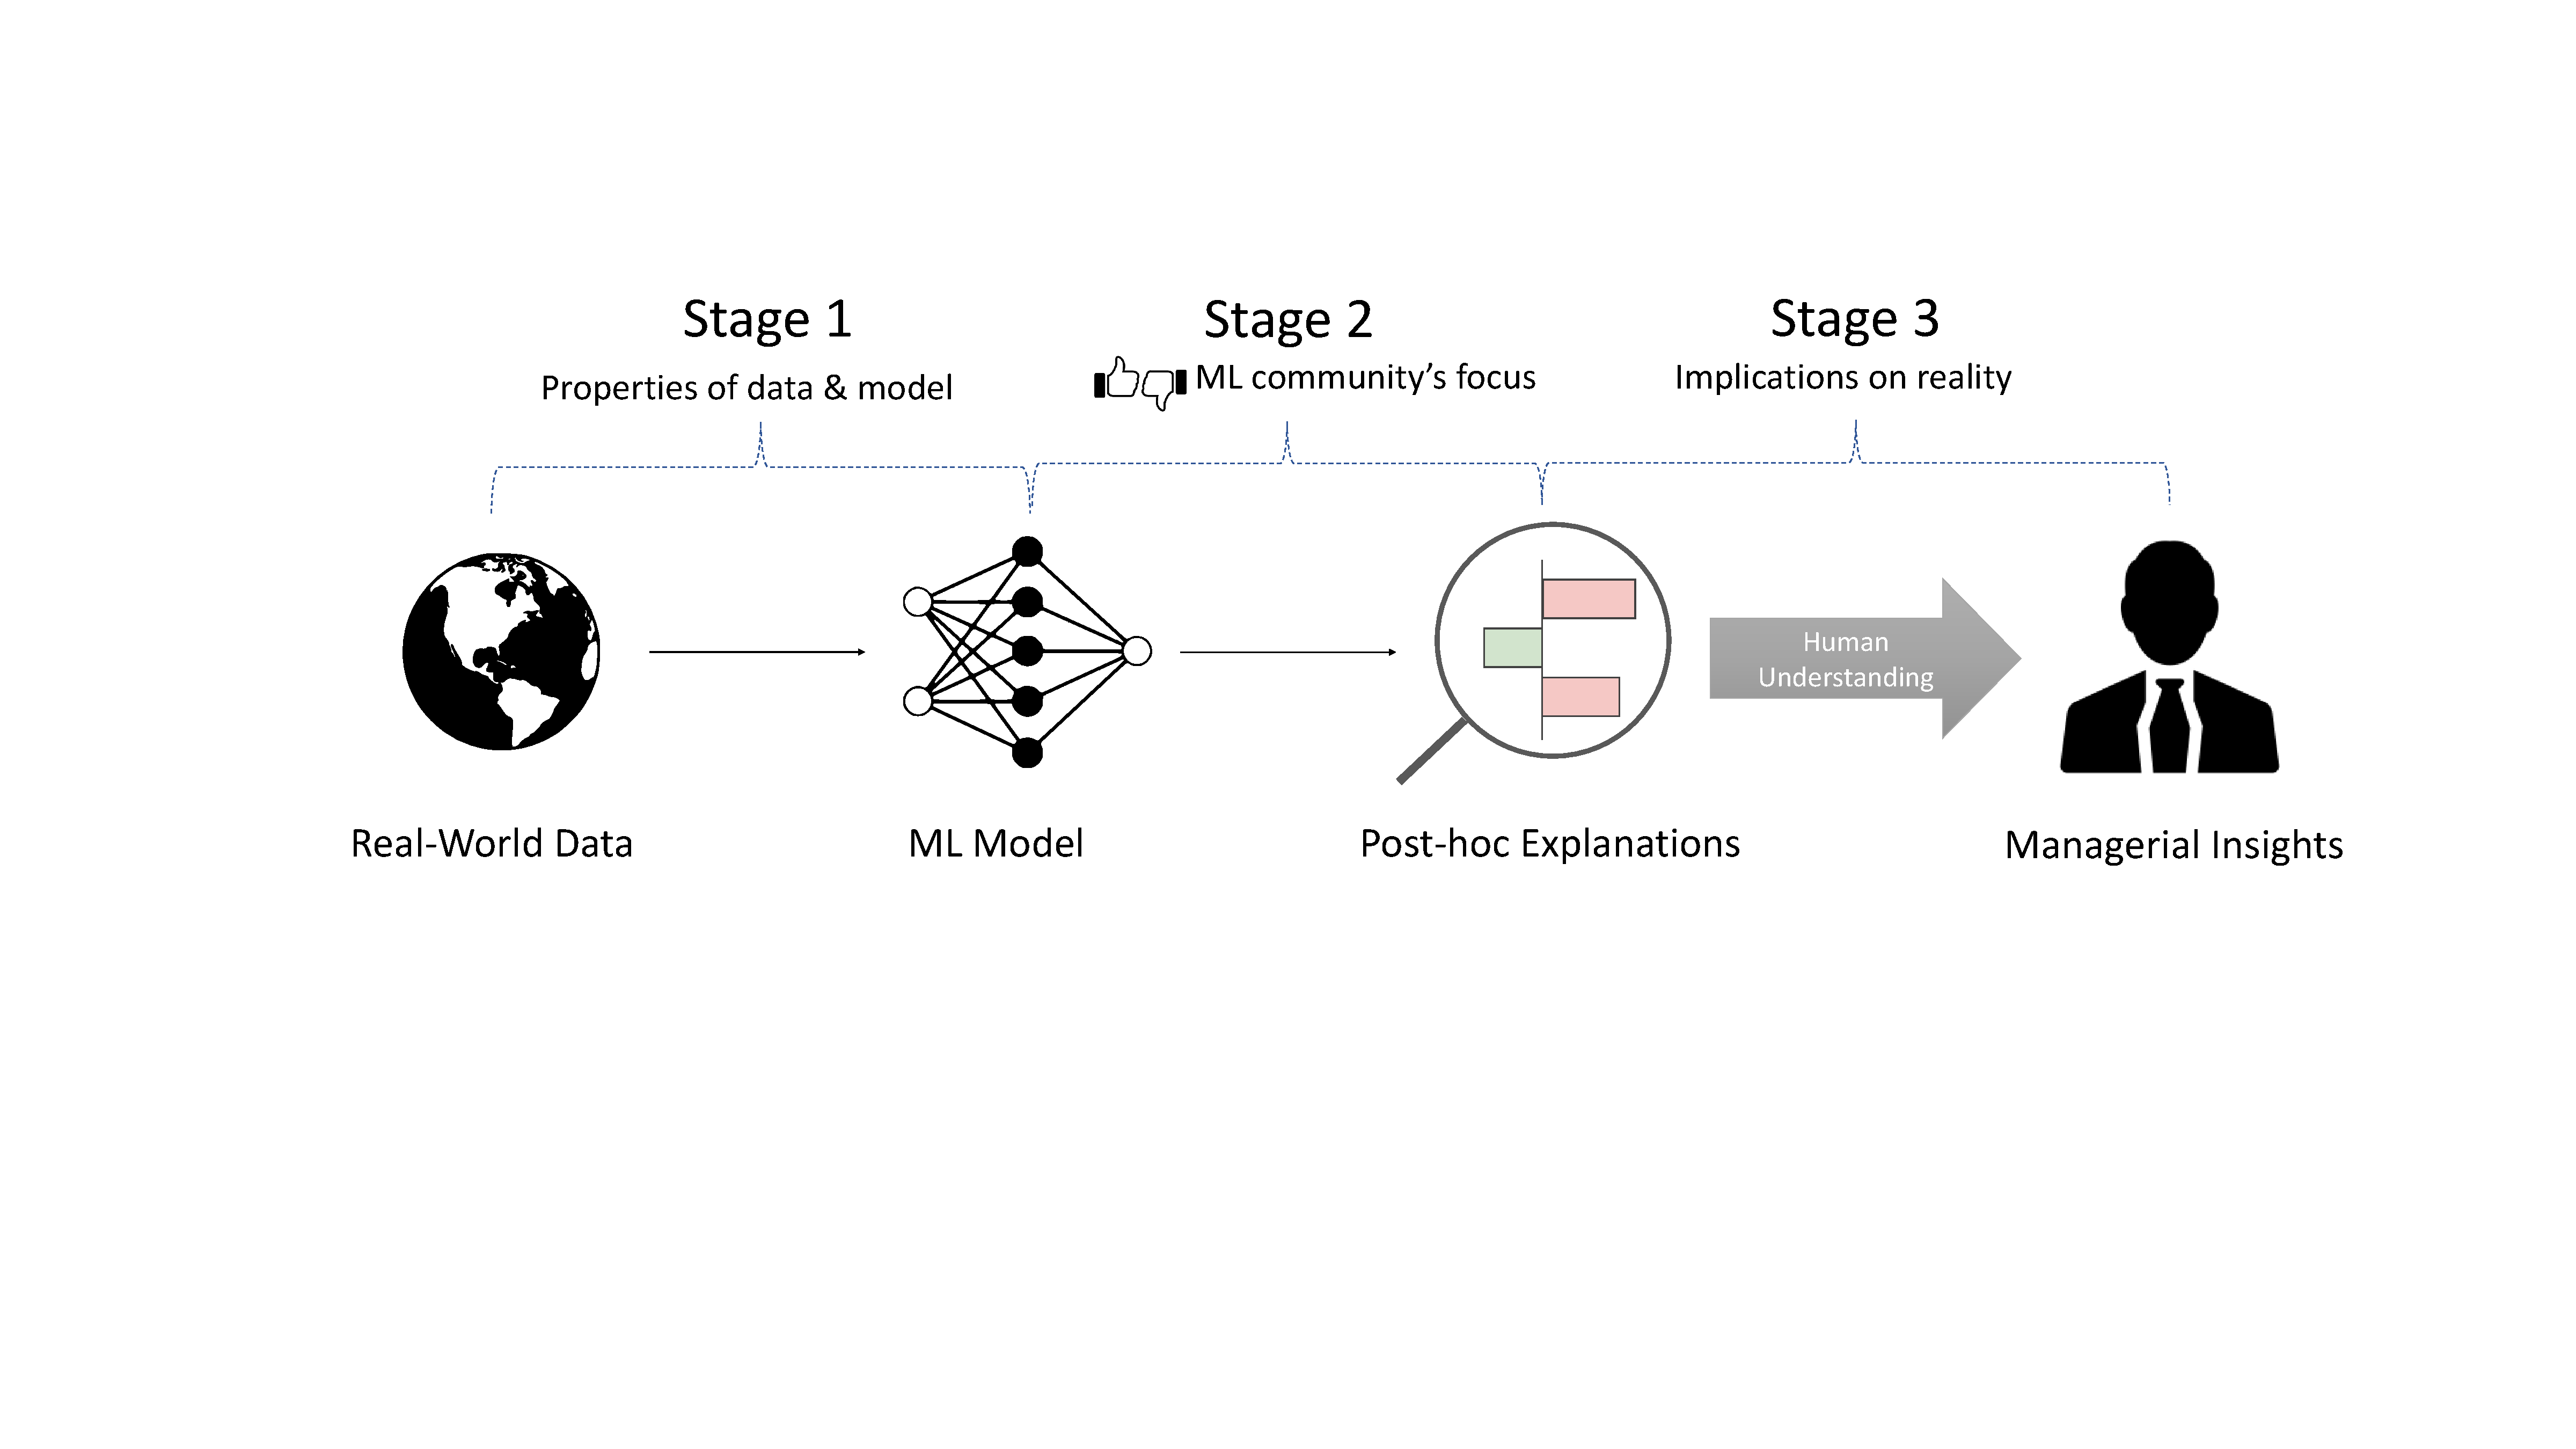
\includegraphics[width = \textwidth,trim=250 500 150 250 mm, clip=true]{Figures/pipeline.pdf}}
        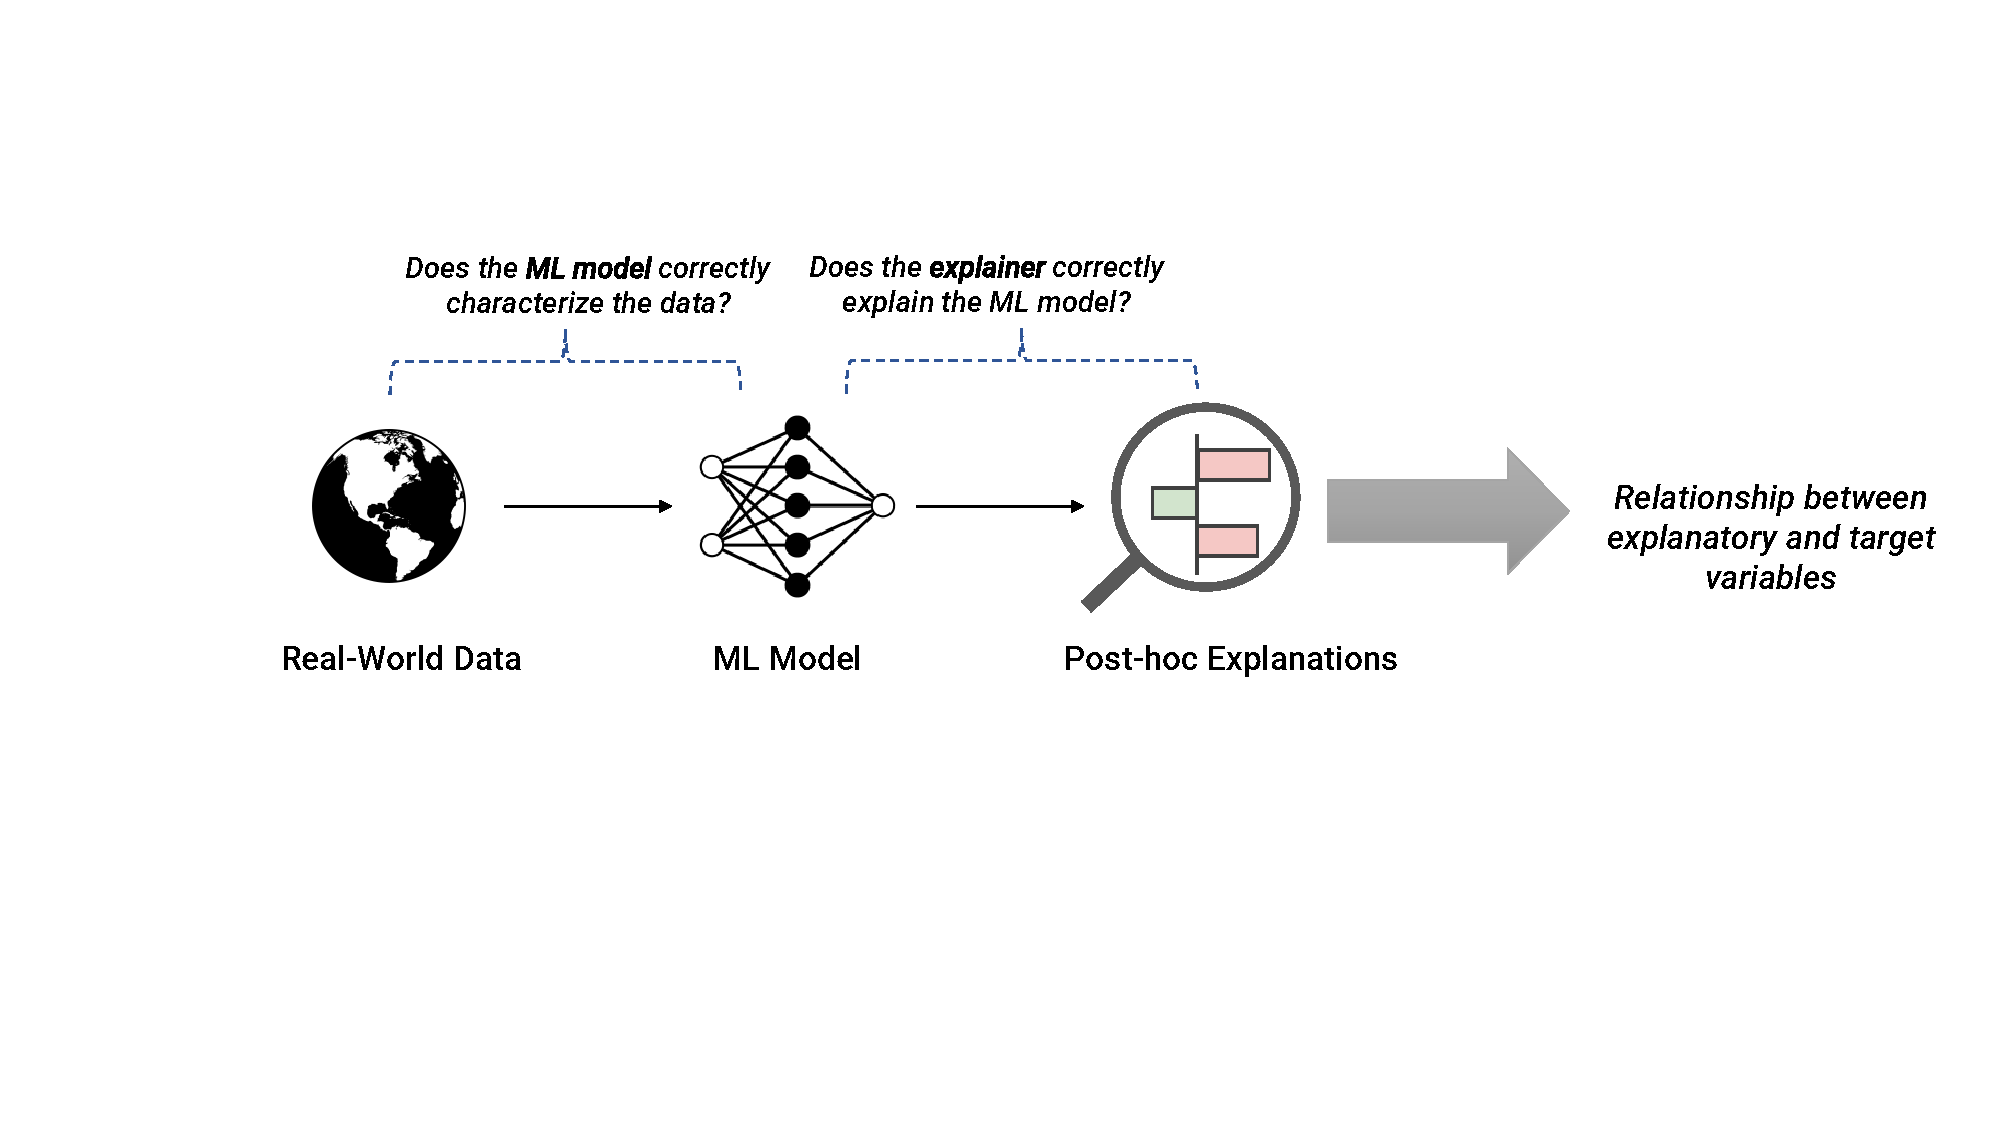
\includegraphics[trim={4.75cm 7.5cm 1.125cm 4.25cm},clip, width = 0.9\textwidth]{Figures/pipeline_flow_new.pdf}
        \caption{Explanation Pipeline: the pipeline of using post hoc explainers to explain a machine learning model. Additionally inferring information about the actual marginal effects of the features constitutes mistaken usage of the pipeline.}
        \label{fig:pipeline}
    \end{figure}
     % They build a black box ML model for a complicated task, which could have many variables, or strong interactions of variables, or include unstructured data, such that canonical econometric methods do not easily apply. Then a post hoc explainer is used to generate feature importance for the ML model,  from which they draw some conclusions on the features as if they are using $\boldsymbol{\beta}$s. 
 

 
 % In addition, there are many types of feature importance \citep{AchenChristopherH1982Iaur}. However, except for \citep{lorentzen2020peeking}, the works cited in the previous paragraph did not provide a formal definition of feature importance and justify that the explainer(s) used were actually providing that type of feature importance. Similarly, the basic question of why Shapley values are appropriate feature importance measures is never addressed in these works\footnote{It is argued in \citep{kumar20shap} that Shapley values are not conducive to human understanding of feature importance.}. 


%Therefore, the goal of this paper is to urge the research community to approach post hoc explanations with skepticism and a more critical eye. 
% We argue in this paper that there exist fundamental flaws in using post hoc explanations to elicit information on $\boldsymbol{\beta}$s. 
Therefore, the goal of this paper is to conduct a thorough investigation into this new and emerging trend of research methodology. We aim to directly answer the question, 
``\emph{Can SHAP and LIME explanations capture the correct relationship between $X$ and $Y$, specifically the marginal effect of $X$ on $Y$, in the data?}''
with both empirical and theoretical evidence.  Specifically, we investigate whether the SHAP and LIME explanations align with the true marginal effects in the data within the three contexts that they are often used in, as described previously. For this purpose, we design three \textit{new} metrics that assess post hoc explanations in terms of capturing correct information about the true marginal effects. The first metric evaluates whether an explanation's feature importance values have the same signs as the corresponding marginal effects. We call it the \textbf{directionality} of an explanation, since it represents how well an explanation identifies the directions in which features influence the target. The second metric evaluates how much the ranking of features by a post hoc explanation agrees with the ranking induced by the marginal effects. We call it the \textbf{concordance} of an explanation. The last metric evaluates whether a post hoc explanation identifies the most important features. We call it the \textbf{relevance} of the explanation. These metrics assess the extent to which the explanations are consistent with the marginal effects in terms of the sign, the ranking of features, and the identification of the most important features. We call the evaluation of these three metrics the test of \textbf{data-alignment}.

We evaluate the data-alignment of post hoc explanations using simulated data where we know and can control the ground truth marginal effects in the data. We set our ground truth models to be linear because the extent an explainer can produce data-aligned explanations of simple linear models is  indicative of its potential for data-alignment in more general scenarios -- if an explainer cannot give data-aligned explanations of simple linear phenomena, it is very likely unable to be able to explain the complex processes underlying practical datasets. Unfortunately, our findings reveal that SHAP and LIME explanations typically \textit{do not align} with the marginal effects, not even qualitatively (directionality), and the alignment further drops as the feature dimension increases. This misalignment is evident even in straightforward business scenarios with a linear ground truth model and when the black box model being explained demonstrates high predictive performance on data containing all relevant features to $Y$, all of which are mutually independent. 

We then delve into the causes of this misalignment, discovering that various factors within the explanation pipeline affect explanation quality. These include having correlated features in the data, the predictive performance of the black box model, and specific settings of explainer model parameters. %We corroborate the initial presentation of our results by showing that misalignment pervades an additional 100 simulations where we explain models produced using AutoML that were trained on datasets with varying numbers of features, rows, and label noise.
Critically, we offer a theoretical justification for why SHAP explanations inherently fail to align with the marginal effects, making Shapley values fundamentally inappropriate for any definite claims regarding marginal effects. We show that SHAP estimates situational importance~\citep{StrumbeljErik2014Epma}, 
 which expresses the consequence of a feature taking on a value different from its mean. Although the computation of situational importance for a feature involves its marginal effect, the information it contributes can be destroyed in the process. Furthermore, we present theoretical grounds for conditions under which LIME might achieve a high degree of data-alignment.

% \textcolor{red}{I think we should say SHAP and LIME separately. }

% We then demonstrate another critical issue of post hoc explanations: inconsistency. Inconsistency refers to the difference in explanations produced by different configurations within the Explanation Pipeline. Using the same simulated data, we show that varying choices along this pipeline can lead to significantly divergent, and occasionally opposing, explanations. It then follows from the view that the purpose of science is to identify phenomena that occur without fail that post hoc explainers have very limited utility to researchers.


Finally, we explore potential strategies to increase the data-alignment of explanations provided by SHAP and LIME. Although our theoretical and empirical findings suggest that it is not possible to fully eliminate the issue of data-misalignment, they nevertheless reveal opportunities for improvement, which we address. For instance, for SHAP, the most immediate way to increase data-alignment is to divide its Shapley values by the differences between the corresponding feature values and their means; for LIME, increasing some hyperparameters will significantly increase the alignment with the data.
Another strategy that showed promise involves averaging the explanations derived from a family of accurate models. We also observe that when the training data used by a black box model include all relevant features, all of which are independent, the alignment of explanations of the black box's predictions with the ground truth tends to increase. This suggests that the underlying data quality and structure play a significant role in the effectiveness of post hoc explanations.
However, other intuitive strategies we tested, such as combining explanations from both SHAP and LIME for a single black box model, did not yield effective results. This highlights the complexity of the issue and the need for more nuanced solutions.
It is also important to note that while our proposed mitigation strategies improve data-alignment to various degrees, they do not completely resolve the issue of misalignment inherent in SHAP and LIME. Consequently, post hoc explainers such as SHAP and LIME should be used with great caution by business researchers, and the appropriate uses of such tools need to be clarified.


Overall, our paper identifies and cautions against a growing trend of the inappropriate use of post hoc explanations to draw inferences about data, leading to data misinterpretation. We argue that post hoc explanations should not be used to \textbf{validate} hypotheses about data; instead, their role in gathering knowledge about data should be limited to \textbf{proposal} of hypotheses. To gain an accurate understanding of the underlying relationships  the data, we emphasize the need for more rigorous and comprehensive follow-up analyses, both quantitatively and qualitatively. This distinction is essential to ensure the prevention of the overestimation of the reliability and validity of insights derived from post hoc explainers in business research.


    The paper is organized as follows. We will review related work pertaining to SHAP, LIME, and their weaknesses in Section \ref{sec:related_work}. Section \ref{sec:use_in_b_research} focuses on the use of SHAP and LIME in business literature, showing the prevalence of inappropriate usage. Then we use a simulated dataset with ground-truth models that we created to demonstrate the Explanation Pipeline and its vulnerabilities in Section \ref{sec:pipeline_demo}.  We provide theoretical and empirical analyses on why post hoc explanations are not suitable to infer information about marginal effects in Section \ref{sec:misalignment}. 
    We then showcase some mitigation strategies for SHAP and LIME in Section \ref{sec:mitigation_strategies} and subsequently gauge how beneficial they are over baselines in reproducing the findings of an econometric study carried out using real loan application data in Section \ref{sec:case_study}. The paper concludes in Section \ref{sec:discussion} with a summary of our findings and final remarks on post hoc explanations and their appropriate use in business research. In the appendix, we provide additional details about our experimental designs and  corroborate results of Section \ref{sec:causes_of_misalignment} by repeating the experiment on another dataset.% \tw{do we have mitigation tested on a new dataset as well? if so we should say it}
    
\section{Related Work}
    \label{sec:related_work}
    This section introduces SHAP and LIME and then reviews the prior literature that discusses their weaknesses from perspectives different from our paper. %Weaknesses discussed include intrinsic (theoretical) issues due to how the explainers are designed, and practical issues users may face due to those intrinsic issues. 

    \subsection{Post Hoc Explainers - SHAP and LIME}
     SHAP \citep{lundberg17shap} and LIME \citep{ribeiro16lime}  are the two most widely used model-agnostic post hoc explainers. %Model agnosticism refers to the ability to explain any ML model without the access to the internals of the ML model, i.e., only using the input and output of a model. Attributive explainers explain the predictions of a predictive ML model by attributing numerical feature importance values to each input feature. Both SHAP and LIME represent feature importance using the coefficients of an additive feature importance model. %Counterfactual explainers such as WachterCF\citep{wachter17wachtercf} and DiCE\citep{mothilal20dice} are of secondary importance and explain an output of an ML model by providing a contrasting input that cause the model to produce a different output. 
        We use SHAP and LIME as representatives for post hoc explainers in this paper because they are also the dominant choices for post hoc explainers in business research.

        % Counterfactual explainers explain an output of an ML model by providing a contrasting input that cause the model to produce a different output. It is desirable for the contrasting input to be as close to the original as possible in order to identify a minimal change that yields a different output. Examples of counterfactual explainers include WachterCF\citep{wachter17wachtercf} and DiCE\citep{mothilal20dice}.
        
     %SHAP and LIME are model-agnostic attributive post hoc explainers. They are model-agnostic in the sense that they can explain any ML model.  Standard implementations of SHAP and LIME can explain both classification and regression models using tabular, text, or image data as input.


SHAP (SHapley Additive exPlanations) is a groundbreaking approach in the field of interpretable machine learning that offers a unified measure of feature importance. Developed by Lundberg and Lee in 2017, it builds on the concepts of game theory, particularly the Shapley value, to assign an importance value to each feature for a particular prediction. The fundamental idea behind SHAP is to assess the contribution of each feature to the difference between the actual prediction and the average prediction over the dataset. One of the unique aspects of SHAP is its consistency and local accuracy. The method guarantees that if a model changes in a way that makes a feature more important, the SHAP value of that feature will not decrease. Local accuracy ensures that the contributions of all features sum up to the actual prediction minus the average prediction, providing a detailed and accurate decomposition of the prediction. Note that LIME does not have this local accuracy property. There are several variants of SHAP, such as Kernel SHAP \citep{lundberg17shap}, TreeSHAP \citep{lundberg2018consistent} and DeepSHAP \citep{lundberg17shap}. Each variant retains the core principles of SHAP while adjusting the computational strategy to suit the specific model architecture, ensuring that the interpretability benefits of SHAP can be realized across a wide range of machine learning models.
    % SHAP's additive feature importance model differs from LIME's in that the coefficient of each feature represent the Shapley value~\citep{shapley97shapley} of that feature. SHAP surrogate models are not fit on sampled training data instances directly like LIME's, but rather on sampled coalition vectors (binary vectors indicating presence of each feature). Shapley values were originally a game-theoretic notion meant to quantify how much each player contributed to the final score of a game. In the context of SHAP, the Shapley values (surrogate model coefficients) represent how much the value of the feature to which they correspond contributes to the final value of the black box model's prediction. 

    
 % Underlying LIME explanations are ridge regressors fitted on data sampled around the input datum being explained. 
Although not used as widely as SHAP in business research, LIME is the very first model-agnostic post hoc explainer. It was developed by \citet{ribeiro16lime}. LIME trains a ridge regressor on a synthetic dataset constructed by sampling uniformly around the input datum. The coefficients of the ridge regressors indicate the importance of each feature. LIME discretizes numerical features into quartiles to avoid dealing with problems associated with differing scales of features and ensure users do not get confused when interpreting negative weights for negative valued features. The ridge regression's optimization weighs the sampled data with an exponential kernel and includes an $L_1$ (LASSO) penalty. LIME uses the $L_1$ regularization so that the regressor it produces is sparse in the sense that, rather than including all features, only a subset of features that are most influential for predictions near the instance being explained are included. This makes LIME's explanations more concise. The ridge regressors are called surrogate models because they are trained to approximate the predictions of the black box model.
    
    LIME's ridge coefficients are meant to represent marginal effects, but depending on the LIME variant and the model being explained, they are not the gradient of the black box model at the input being explained. \citet{garreau2020looking} proved that the original LIME formulation's coefficients did not, in general, equal the gradient of the black box model at the input being explained. Instead, each feature importance value is proportional to the partial derivative of the black box at the input datum and the proportionality constants differ by feature. \citet{agarwal21clime} showed that a simpler variant of LIME called C-LIME that does not discretize input features and does not perform weighted ridge regression produced coefficients that are proportional to the gradient of the black box model. %Removing discretization allows C-LIME to recover the gradient because otherwise, local information about the black box's decision boundary is destroyed.
    In discretizing features, the data used in LIME's regression problem consists of binary features indicating which bins (quantiles) the feature values of sampled data fall into, which destroys the gradient since the local information about the black box's decision boundary is lost. Moreover, C-LIME drops the ridge penalty because enforcing sparsity opposes the goal of recovering the gradient. In the specific case where the model being explained is linear, C-LIME recovers the coefficients of the linear model. This being the case, in this paper, we choose to disable the discretization setting of LIME throughout the paper to improve the quality of LIME explanations.



    \subsection{The Evaluation of Post hoc Explanations}
        \label{sec:cs_critique}
        The alarm for post hoc explanations had first gone off in the field of machine learning, as researchers questioned the correctness and validity of post hoc explanations. However, the notions of correctness and validity in the ML literature differ from the point of view we take in this paper. The ML community's attention has mainly focused on explanation quality \textbf{with respect to the ML model} since the primary goal of the machine learning field is to develop new models that make better or faster predictions. In addition, they consider factors relating the ability of humans to interpret the explanations, most of which do not fall within the scope of our critique. Thus, the way the ML community evaluates explainers is different from how we evaluate them in this paper.

    
        That post hoc explainers misrepresent the black boxes they explain is a pillar of the ML community's critique. The terms \emph{fidelity} and \emph{faithfulness} are used interchangeably and generally represent the maxims of completeness and soundness outlined by \cite{zhou21evaluating}. An explanation is complete if it is a full characterization of the black box's behavior. An explanation is sound if its characterization is correct.\footnote{In this paper, however, we characterize faithfulness in reference to the ground truth instead of the black box model because we are interested in obtaining insights about reality, not about black box models. In Section \ref{sec:evaluating_faithfulness}, we define metrics that capture our notion of faithfulness.} 
    \cite{garreau2020looking} and \cite{han22which} consider soundness from a function approximation perspective, directly measuring the difference between an explainer  and the black box model. \cite{garreau2020looking} shows that LIME's approximation error is always bounded away from 0. \cite{han22which} analyzes kernelSHAP and LIME relying on a view of KernelSHAP and LIME as kernel weighted linear regression models whose input data are sampled by perturbing the input by random noise. They remark that the choice of noise distribution made by kernelSHAP and LIME prevents them from being able to recover the gradient of linear models they explain as feature importance values. It follows that KernelSHAP and LIME cannot necessarily be expected to reliably perform their intended task of interpreting black box model behaviors. 
Other fidelity/faithfulness metrics measure particular approximation properties such as the extent to which an explainer assigns zero importance to features the model does not depend on are used as metrics in \cite{nguyen2020quantitative}. Metrics such as Deletion and Insertion metrics are based on the idea that features said to be important by an explainer should have significant effects on black box output \citep{deyoung20eraser,nguyen2020quantitative,alvarez18robustness,luss2021leveraging}. However, all previously mentioned papers study the fidelity with respect to the \textit{ML model}, rather than the data, as we do in this paper. Nevertheless, the aforementioned studies partially answer our research question -- if a black box explainer has difficulty even being faithful to an ML model, it would be even more challenging for it to provide correct data insights.
%The underlying supposition of Deletion and Insertion metrics is that removing or adding features said to be important to a prediction by an explainer should change the prediction to change substantially \citep{deyoung20eraser,nguyen2020quantitative,alvarez18robustness,luss2021leveraging}. %Some works evaluate explainers by taking advantage of contexts where feature importance information of a model is known. \cite{blunsom2019can} evaluates explainers of a white box recurrent model by quantifying the explainers' error rates with respect to identifying important tokens in inputs. \cite{carmichael21framework} evaluates additive explainers by calculating the Jaccard index between the sets of effects present in neural networks and GAMs and the effects and associated contributions of features given by explainers for those models. 
    
  The ML community has also largely focused on other aspects of post hoc explanations, such as interpretability or understandability of the explanations. Explainers which satisfy desiderata related to interpretability should be able to provide a description of the behavior of a black box model in a form which can be easily understood by humans. For example, explanations should be simple enough to be intelligible but complex enough so that the explanation is still complete and sound. Parsimony \citep{nguyen2020quantitative} and clarity \citep{lakkaraju2017interpretable,montavon2018methods,alvarez18robustness} metrics, for example, measure the simplicity and ambiguity of explanations, respectively\footnote{We use the terminology of \cite{markus2021role} here.}. \cite{jacovi2023diagnosing} further requires that the form of explanations match what the psychology literature identifies as natural for human understanding.  Simplicity of explanations beyond the per-feature importance values given by attributive explainers is not desirable in our application because, e.g. artificial enforcement of sparsity could encourage explanations to omit information about the marginal effects and become incomplete and unsound as a result. %For example, LIME's use of a LASSO penalty to make its explanations sparse is undesirable because it could cause a feature to have zero importance when the $\beta_j$ for that feature is non-zero. %Futhermore, stability metrics quantify how different explanations of nearby inputs are. The size of the local Lipschitz constant of the function underlying the explainer is one such example \citep{alvarez18robustness}. Stable explanations can be desirable because an explainer's explanations for two similar inputs being very dissimilar could engender mistrust of the explainer or arouse unwarranted suspicion of unfairness in the underlying decision process. These factors, however, are not within the scope of our discussion.

    
   
    
    
    \section{Use of SHAP and LIME in Business Research}
        \label{sec:use_in_b_research}
% \textcolor{red}{find papers that use post hoc explanation to get insights that resemble $\boldsymbol{\beta}$ (explaining G). Also mention that some papers only use post hoc explainer on M. It is the intended use of the post hoc explanations, but even that faces severe criticism from the ML community discusses explanations for M}

% \textcolor{red}{Move the appendix here}
        As part of our literature review process, we cataloged papers at the intersection of business and explainable machine learning.
        
        We searched for papers from three sources. First,  we used Web of Science %and SSRN\footnote{We searched on SSRN because business journal papers usually take a few years to get published so there are many preprints available on SSRN.} 
        to search for publications citing at least one of LIME~\citep{ribeiro16lime} or SHAP~\citep{lundberg17shap} and have either ``LIME" or ``SHAP" appear in the body of the paper. The results were filtered by topics related to business, such as management, economics, supply chain \& logistics, operations research \& management science, etc. More than 700 papers were identified. See Figure \ref{apx_tab:citation_count_graph} for a breakdown of the number of papers by year.
               \begin{figure}[ht]
            \centering
            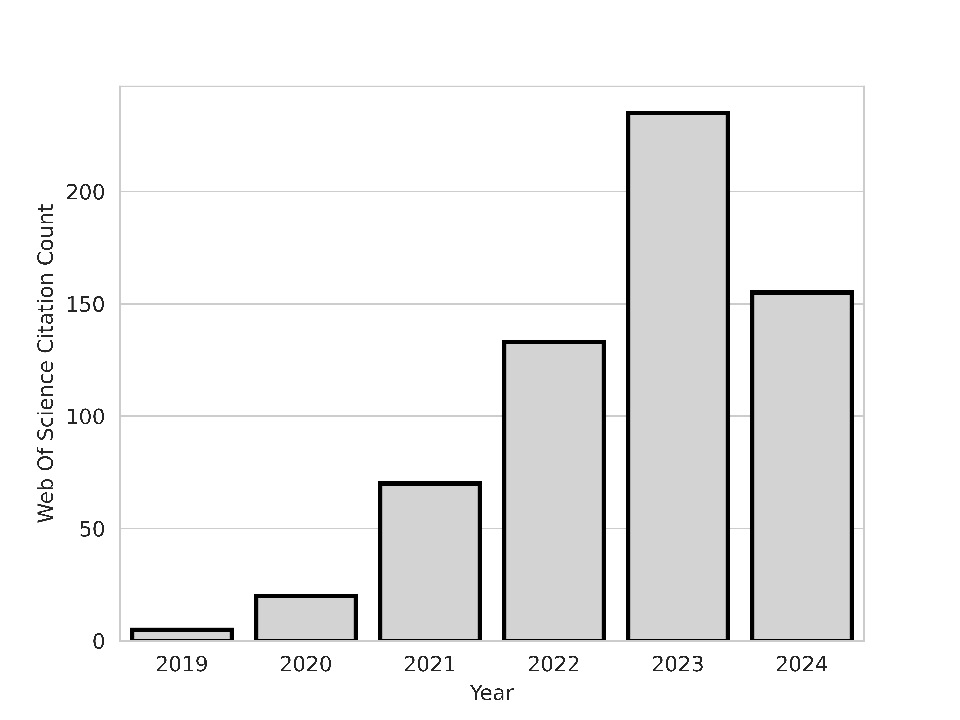
\includegraphics[width=.5\textwidth]{Figures/citation_count_new.pdf}
            \caption{Year-by-year breakdown of number of papers citing either LIME or SHAP that belong to business-adjacent Web of Science categories.}
            \label{apx_tab:citation_count_graph}
        \end{figure} %\tw{I don't like the bar plot. Change the bar plot to gray (black edges and gray fills) }
        The second source of papers is INFORMS journals. We searched with the same keywords on the INFORMS journal portal. Finally, we searched on SSRN for papers that are not published yet. Because business journal papers usually take a few years to get published, there are many preprints available on SSRN. The total number of papers from these three sources that matched our keywords was over 700. 
        
        We then iterated through the resulting papers one by one, collecting papers that actually used SHAP or LIME to explain a machine learning model (many papers only mentioned SHAP or LIME in the context of related work or future work) until we had a total of 150 different papers. 
        Out of these papers, 91\% used SHAP and 14\% used LIME to generate explanations for their models, including 5\% using both of them.


        
        We took a close look at these papers and characterized their use of post hoc explanations by the following procedure. We first searched for evidence that it was understood that the intended use of SHAP and LIME is to explain model outputs (rather than the data). On those that fail this screening, we identified problematic language indicative of inappropriate use of post hoc explanations and recorded quotations of problematic sentences.
        Not all papers contained such language; in some papers it was clear or made explicit that authors used SHAP and LIME only within the scope of model explanation. Having identified any quotations which we deemed problematic, we then divided the papers into three categories: the \textit{controversial} papers that clearly extrapolated explanations to glean information about the marginal effects, the \textit{ambiguous} papers whose wording could suggest extrapolation, and the \textit{proper} papers that only used explanations for model interpretation (the intended use).% Note again, though, that both SHAP and LIME fall short for their indented purpose and face intense scrutiny from the ML community \cite{kumar20shap,garreau2020looking}.

%\textcolor{red}{add a summary of the findings \&statistics from the 116 papers}
%\textcolor{red}{double check and update the numbers}
        We found that 42\% of the papers are controversial - they clearly extrapolated explanations to gain insight into the marginal effects in the data. In addition to that, there is another 15\% ambiguous papers that at least used unclear language such that readers could interpret their findings as being made about the marginal effects. This means that \textbf{more than half} of the papers we sampled had some problematic language. Further, \underline{76\% of the controversial papers were from top journals}.\footnote{A journal was considered a ``top journal" if it is an INFORMS journal or its most recent 5-year impact factor according to Clarivate's Journal Citation Reports (JCR) was at least 5.0 at the time of writing (June 2024).}
        %Given the popularity of SHAP and the idea that the presence of this problem in publications from top journal is indicative of the pervasiveness of the problem, we also separately surveyed papers from the INFORMS family of journals that used SHAP to explain a machine learning model. About 25\% of these papers had clear extrapolations, and 17\% could be construed as having extrapolated. Thus it was still the case that about half of the papers using SHAP contained problematic language.
        We believe that this result is indicative of a rising trend of using SHAP or LIME to gain data insights.

        The interpretation of SHAP and LIME feature importance values in the controversial papers fell into three categories: 1) identifying the directionality of impact of each feature (i.e., feature importance sign), 2) ranking features by relative importance, and 3) identifying a subset of the most important features. Table \ref{tab:metric_examples} below records prototypical ways in which authors expressed their desire to perform these tasks. In Section \ref{sec:evaluating_faithfulness}, we define metrics to characterize the ability of an explainer to perform these tasks. We call them directionality, concordance, and relevance, respectively. 

% ANONYMIZED VERSION
% \begin{table}[htbp]
% \small
% \caption{Correspondence Between Paper Language and Our Metrics. Statements appearing in angle braces $\langle \cdot \rangle$ 
% are meant to make the statements more general. The $X_j$ represent data features and $Y$ represents the outcome of interest.}
% \begin{tabu} to 1\linewidth {  P{3cm} | X[l,m]  }
% \toprule
% \textsc{Purpose} & \textsc{Examples} \\
% \hline
% \textbf{Identifying How Features Impact the Target (Directionality)}
% & ``...Positive SHAP values indicate that the variable has a facilitative effect on $\langle Y\rangle$, while negative values indicate a suppressive effect..." \\ 
% & \vspace{-.8cm}``...Individuals whose predictions received larger SHAP values for this feature are more likely to have $\langle Y=1\rangle$..."\\
% & ``...Choosing features with positive mean SHAP are recommended options because they have positive effects on $\langle Y\rangle$..." \\
% \hline
% \textbf{Ranking the Features by Relative Importance (Concordance)}
% & ``...This study provides insights for planning the design of $\langle X\rangle$ by assessing the relative importance and associated rankings of the $\langle X_j\rangle$ in predicting $\langle Y\rangle$..."\\\smallskip
% & \vspace{-1.3cm}``...The use of Shapley values enables us to identify and rank relevant $\langle X_j\rangle$ for the investigated $\langle Y\rangle$.."\\\smallskip
% & \vspace{-.7cm}``...Our feature rankings and visualizations of impact patterns provide policy makers with evidence for strategies to improve $\langle Y\rangle$..." \\
% \hline
% \textbf{Identifying the Most Important (Top-$k$) Features (Relevance)\hspace{3cm}}
% & ``...That $\langle X_1$, $X_2$, and $X_3\rangle$ have the top-3 SHAP values and that their SHAP values are positive reveals that increasing $\langle X_1$, $X_2$, and $X_3\rangle$ would lead to larger $\langle Y\rangle$..."\\\smallskip
% & \vspace{-.8cm}``...We use SHAP explanations of an XGBoost Classifier to identify the key features which contributing to the risk $\langle Y\rangle$..."\\\smallskip
% & ``...By using XAI to identify the most important factors and indicators that contribute to $\langle Y\rangle$, their values and fluctuations can then be monitored over time..." \\
% \hline
% \textbf{Other Usage}
% & (\textbf{OLS Alternative}) ``...The combination of a black box algorithm and SHAP provides similar economic insights as provided by pooled OLS..."\\\smallskip
% & (\textbf{Theory Confirmation}) ``...SHAP is used to interpret the quantitative associations found by XGBoost; our results provide empirical support for prior theoretical findings..."\\\smallskip
% & (\textbf{Recourse Advocacy}) ``...Since $\langle X_1$, $X_2$, and $X_3\rangle$ have high SHAP importance and substantial effects on $\langle Y\rangle$, $\langle X_1$, $X_2$, and $X_3\rangle$ should be given attention by policy makers to increase $\langle X_1$, $X_2$, and $X_3\rangle$..." \\
% \bottomrule
% \end{tabu}
% \label{tab:metric_examples}
% \end{table}


\begin{table}[htbp]
\small
\caption{Correspondence Between Paper Language and Our Metrics. Statements appearing in angle braces $\langle \cdot \rangle$ 
are meant to make the statements more general. The $X_j$ represent data features and $Y$ represents the outcome of interest.}
\centering

    \begin{tblr}{width=1.0\textwidth, colspec={X[c,m,3cm]|X[l,m]}}
%X@{} | X[l,m]  }
%\toprule
\textsc{Purpose} & \textsc{Examples} \\
\hline
\textbf{Identifying How Features Impact the Target (Directionality)} & {$\bullet$ ``...Positive SHAP values indicate that the variable has a facilitative effect on $\langle Y\rangle$, while negative values indicate a suppressive effect..." \\ 
$\bullet$ ``...Individuals whose predictions received larger SHAP values for this feature are \\ more likely to have $\langle Y=1\rangle$..."\\
$\bullet$ ``...Choosing features with positive mean SHAP are recommended options \\ because they have positive effects on $\langle Y\rangle$..." \\} \\ \hline
\textbf{Ranking the Features by Relative Importance (Concordance)}
& \makecell[l]{$\bullet$ ``...This study provides insights for planning the design of $\langle X\rangle$ by assessing the \\ relative importance and associated rankings of the $\langle X_j\rangle$ in predicting $\langle Y\rangle$..."
\\$\bullet$ ``...The use of Shapley values enables us to identify and rank relevant $\langle X_j\rangle$ \\for the investigated $\langle Y\rangle$..."
\\$\bullet$ ``...Our feature rankings and visualizations of impact patterns provide \\policy makers with evidence for strategies to improve $\langle Y\rangle$..."} \\ \hline \SetCell{m} \textbf{Identifying the Most Important (Top-$k$) Features (Relevance)}
& \makecell[ml]{$\bullet$ ``...That $\langle X_1$, $X_2$, $X_3\rangle$ have the top-3 SHAP values and that their SHAP \\values are positive reveals that increasing $\langle X_1$, $X_2$, $X_3\rangle$ would lead to larger $\langle Y\rangle$..."\\
$\bullet$ ``...We use SHAP explanations of an XGBoost Classifier to identify the key \\features which contributing to the risk $\langle Y\rangle$..."\\
$\bullet$ ``...By using XAI to identify the most important factors and indicators that \\contribute to $\langle Y\rangle$, their values and fluctuations can then be monitored over time..."} \\ \hline
 \SetCell{m} \textbf{Other Usage}
 & \makecell[ml]{(\textbf{OLS Alternative}) $\bullet$ ``...The combination of a black box algorithm and SHAP \\provides similar economic insights as provided by pooled OLS..." \\
 (\textbf{Theory Confirmation}) $\bullet$ ``...SHAP is used to interpret the quantitative \\associations found by XGBoost; our results provide empirical support \\ for prior theoretical findings..." \\
(\textbf{Recourse Advocacy}) $\bullet$ ``...Since $\langle X_1$, $X_2$, and $X_3\rangle$ have high SHAP importance \\and substantial effects on $\langle Y\rangle$, $\langle X_1$, $X_2$, and $X_3\rangle$ should be given attention by \\ policy makers to increase $\langle X_1$, $X_2$, and $X_3\rangle$..."} \\
%\bottomrule
\end{tblr}

\label{tab:metric_examples}
\end{table}



\section{Explanation Pipeline}
    \label{sec:pipeline_demo}
In this section, we formulate an Explanation Pipeline based on the approaches commonly employed in the business literature to obtain explanations using post hoc explainers. We then use a simulated dataset to demonstrate how this pipeline is typically applied.
    
An explanation pipeline consists of two stages. In the first stage, which we call the \emph{prediction stage}, a machine learning model $\mathcal{M}$ is trained on data $\mathcal{D}$. This stage addresses the prediction problem, with the resulting predictions being evaluated using various metrics such as accuracy, ROC, and others. Evaluations with respect to these metrics are often the primary results in many business papers that solve a prediction task. In the second stage, which we call the \emph{explanation stage}, an explainer model (e.g., SHAP or LIME), denoted by $\mathcal{E}$, is applied to $\mathcal{M}$ to generate explanations. We denote an explanation for feature $X_j$ of $\mathcal{E}$'s prediction for the $i^{\text{th}}$ data instance $\mathbf{x}^{(i)}$ as $e_{\mathcal{E}}(x^{(i)}_j)$. This stage provides model interpretation through simple human understandable explanations such as feature importance. % We will also use the notation $\mathbf{x}^{(i)}$ to represent test set instance $i$. % building a machine learning
    
    We illustrate the Explanation Pipeline with a simulated loan approval dataset.\footnote{Real datasets are less suitable for the experiments in this paper because we require access to the ground truth in order to evaluate the faithfulness of the post hoc explanations. However, in Section \ref{sec:case_study}, we will conduct a case study using a real loan application dataset and use the results of a published econometric study using that dataset as the ground truth.} Our simulation models the task of predicting whether an individual will be approved for a loan based on their demographic features and credit-related features. We define a model for generating the target variable so that the ground truth is known and controllable. We also define the ground truth model to be linear, such that the explanation task is relatively easier for the post hoc explainers. %Some of the features are not independent. We demonstrate in Section \ref{sec:role_of_correlation} that the lack of feature independence effects data-alignment. This being the case, we test our mitigation strategies in Section \ref{sec:mitigation_strategies} using a variant of the data generation process where all features are mutually independent in order to control for the effect of feature correlation and focus on the effect of our mitigations.                                       
    In the following, we will describe how we generate our data and then apply the pipeline to a sample dataset using SHAP for demonstration. For consistency, we will be using this dataset and its variant in Section \ref{sec:misalignment} as well. %until Section \ref{sec:role_of_correlation}, where we introduce a variant of the dataset which has only mutually independent features and used thereafter. %For example, in section \ref{sec:stage_2}, we will add confounding features to see how model explanations are affected by data that do not satisfy conditions for causal inference. Below, we show the different stages of our Explanation Pipeline.

 \subsection{Data Generation Process}
 \label{sec:data_generation}
 % \paragraph{Data Generator $\mathcal{G}$}
 %In this section, we will introduce a simulated dataset, variants of which will be used throughout the paper.  
 % thus the coefficients in the linear model are used for the ground truth. %The ground truth model is linear, so we can evaluate local explanations with respect to the ground truth's global explanation. 
 Our data generation process simulates a process of deciding whether loan applications are approved in a real-world scenario. In it, applicants have a total of ten features: four demographic features and six credit-related features. Table \ref{tab:simulated} summarizes how each feature is generated. % We also include an unobserved confounder to enhance the realism of the dataset - this feature is used to generate the label but not observed by $\mathcal{M}$. % The meanings and manners of construction of all the features are reported in Table \ref{tab:simulated}. 
 The credit score feature is generated based on a partial FICO credit scoring model \citep{ligons_fico} and is given by the following formula: $\text{Credit Score}= 650 + (10 + 2.5\cdot \text{Credit History}) + (70 - 15 \cdot \text{Inquiries}) + (35 - 4 \cdot \text{Delinquencies}) + (105 - 100 \cdot \text{Utilization})$.  ``Cosigner" is positively correlated with ``Married" in that the probability of having a cosigner is given by $\sigma(2\cdot \text{Married} + 1 + \epsilon)$ where $\epsilon \sim \mathcal{N}(0,\frac{1}{2})$. 
\begin{table}[ht]
\centering
\resizebox{\textwidth}{!}{%
\begin{tabular}{l|l|l}
\toprule
\textsc{Feature} & \textsc{Meaning}                           & \textsc{Formula}       \\ \toprule
Age              & Applicant Age                                   & Uniform(18,100)        \\ 
Sex              & Applicant Sex                                   & Bernoulli(.5)          \\
Married          & Applicant Marital Status                        & Bernoulli(.5)          \\ 
Income           & Applicant Income                                & Normal(40,000, 30,000) \\ 
Inquiries        & Number of credit inquiries                      & Uniform(0,6)           \\ 
Cosigner         & Indicator of presence of loan cosigner & Function of Married         \\ 
Utilization      & Proportion of total credit utilized            & Uniform(0,1)           \\ 
Delinquencies    & Number of delinquent  payments in last 2 years & Uniform(0,24)          \\ 
Credit Score     & Credit score based on FICO scoring & FICO credit scoring model  \citep{ligons_fico}            \\ \bottomrule
\end{tabular}%
}
\caption{Description of features for simulated loan data.}
\label{tab:simulated}
\end{table}


  % As aforementioned, we designed the underlying true model $\mathcal{G}$ that determines whether individuals are approved for a loan. The decision is based on all features but the unobserved social support feature. Social support is an unobserved confounder of ``Cosigner." In subsequent sections, we will adapt the dataset depending on what is needed for each experiment. In one experiment, for example, we will compare what happens to explainers when their dataset does and does not have an unobserved feature. 

   We define a model $\mathcal{G}$ for generating applicants' labels, \textit{approved}, or \textit{rejected}, so that we have a ground truth model that we can use to evaluate the quality of explanations from the explainers. This ground truth model represents the underlying decision-making process that is never observed.  We define $\mathcal{G}$ as a linear model and then compose it with a logistic sigmoid function to generate the labels. The true marginal effects $\boldsymbol{\beta}$ are defined using $\mathcal{G}$\footnote{Note, however, that under our definition of marginal effects, the coefficients in $\mathcal{G}$ can differ from $\boldsymbol{\beta}$ because the $\beta_j$ for a feature which influences other features is defined to be the total derivative of the response with respect to that feature.} below; it is the ground truth we compare the feature importance values provided by SHAP and LIME against.
   
    $\mathcal{G}$ is defined as the following linear model taking standardized features as input. 
    % \textcolor{red}{$\mathcal{G}$ has to use all features somewhere in the paper, if not section 3 then section 4 and 5 for demonstrating some issues. If there are features in Table 2 not used by G ever, remove it}
    %\begin{tcolorbox}%[title = Ground Truth Model $\mathcal{G}$]
    \begin{equation}
    \label{eqn:gt}
    \begin{split}
    \mathcal{G}(X) =2.5 +.0005\cdot\text{Age} -0\cdot\text{Sex} +.1 \cdot \text{Married} + .25\cdot \text{Cosigner} + 1.5 \cdot \text{Credit History} + \\   3 \cdot \text{Income} - 1\cdot\text{Utilization} -.75 \cdot \text{Delinquencies} - .5\cdot\text{Inquiries} + 5.\cdot\text{Credit Score} + \epsilon,
    \end{split}
    \end{equation}
    %\end{tcolorbox}
    \noindent where $\epsilon \sim \mathcal{N}(0,\frac{1}{4})$ captures all the variation in the response variable that is not explained by the explanatory variables.
    Using the logistic sigmoid function $\sigma(\cdot)$, we assign $Y = 1$ (approved) for cases with $\sigma(\mathcal{G}(\mathbf{x}))\geq 0.5$, and $Y = 0$ (rejected) otherwise. The intercept term $2.5$ is chosen so that at a baseline when feature values are zero (features are standardized, so the means of numerical features are zero), an applicant is most likely accepted. The remaining coefficients are chosen so that ``Credit Score" is the most important feature, followed by ``Credit Inquiries," ``Delinquencies," ``Income," ``Credit History," ``Married," ``Cosigner," ``Age" and finally ``Sex." These coefficients are motivated by the literature. The probability of being approved for a loan increases significantly with an applicant's credit score and insignificantly with their age \citep{cfb_age}. The probability decreases significantly as applicants use higher proportions of their available credit and receive recent credit inquiries. The sex of a customer is not supposed to effect approval outcomes~\citep{Calcagnini2014}. 
   We then create a dataset $\mathcal{D}$ with 5000 data points by sampling from the distributions of features to simulate applicant profiles ($\mathbf{X}$) and using $\mathcal{G}$ to create the labels ($Y$).  
   In the following, we apply the Explanation Pipeline to demonstrate how one obtains a post hoc explanation by explaining $\mathcal{M}$ using $\mathcal{E}$. 


\subsection{Applying the Explanation Pipeline}
\label{sec:applying_to_simulated}
The Explanation Pipeline consists of two stages, the \emph{prediction stage} in which an ML model $\mathcal{M}$ is built using $\mathcal{D}$, and the \emph{explanation stage} in which outputs of $\mathcal{M}$ are explained with an explainer $\mathcal{E}$. 

To demonstrate the pipeline, we choose $\mathcal{M}$ to be a neural network (NN) with 100 hidden layer nodes. We perform a standard 80-20 train-test split of the 5000 applicants. The accuracy of $\mathcal{M}$ is 0.86 and the AUROC is 0.93 on the test set. We choose $\mathcal{E}$ to be SHAP for demonstration purpose since SHAP is used much more often than LIME is. %Unless otherwise stated later in the paper, this model is what $\mathcal{M}$ refers to. 
%Then we use SHAP to explain $\mathcal{M}$'s decision on one applicant.% in hopes of learning about the marginal effects underlying the data, i.e., the coefficients in $\mathcal{G}$.% We do not allow LIME to discretize the input features to give it a better chance of recovering $\boldsymbol{\beta}$ (recall from Section \ref{sec:related_work} the comparison of default LIME and C-LIME)\footnote{We show in the Appendix that allowing discretization makes LIME's results demonstrably worse.}. %Since LIME builds a linear model locally for the focal instance being explained, the coefficients of LIME's linear model and the ground-truth coefficients can be compared to evaluate how faithful LIME is to the ground truth.
We demonstrate a SHAP explanation using one applicant that we will call John. John is a 61-year-old married male who makes approximately \$66,000/year, has a credit score of 761, 6 credit inquiries in the past 6 months, and utilizes 19\% of his 28-month old line of credit. He also has a cosigner and no delinquent payments in the last two years. John's application was accepted, that is, $Y = 1$. Since we design the data generation model $\mathcal{G}$, we know the ground truth marginal effect of each feature in obtaining John's application outcome, following formula (\ref{eqn:gt}), shown in the left panel of Figure \ref{box}. John's feature values are shown in Figure \ref{fig:shap_ex_feat} and shapley values returned by SHAP  are visualized in Figure \ref{box}. We denote them by $e_\text{SHAP}(x_j)$. %For the most part, it was because their credit score is too low. We will now see if LIME can produce this insight.

 % \begin{figure}[ht!]
 %     \centering
 %     \includegraphics[width=.48\textwidth]{Figures/shap_ex.png}
 %     \caption{}
 %     \label{fig:shap_ex}
 % \end{figure}
\settowidth\mylenC{\textbf{$\mathcal{M}=\text{\textbf{XGBoost}}$}} 
% determine usable width of cols 2 and 3:
\setlength\mylenD{(.3\linewidth-3\tabcolsep)/3}
    \begin{figure}[ht!]
    \small
        \centering
            \begin{subfigure}[t]{.35\textwidth}
              \centering
              %\includegraphics[height=.5\linewidth]{Figures/shap_ex_feat.png}%}%{Figures/feng_fig/acc_increase_iter_2.png}
                \begin{tabular}[b]{l|l}
                \toprule
                \textbf{Feature} & \textbf{Value} \\ \hline
                Credit Score     & 761            \\
                Income           & \$66,000       \\
                Credit History   & 28 months      \\
                Cosigner         & Yes            \\
                Married          & Yes            \\
                Age              & 61             \\
                Sex              & Male \\
                Inquiries        & 6              \\
                Delinquency      & 0              \\
                Utilization      & 19\%           \\
                \bottomrule
                \end{tabular}
                \normalsize
              \caption{John's feature values}
              \label{fig:shap_ex_feat}
            \end{subfigure}%
            \hfill%#space{1cm}
            \begin{subfigure}[t]{.6\textwidth}
              \centering
\begin{tcolorbox}[tabular = {*{6}{wc{\mylenD}}}, hbox,center,label = {pipelines_3_ex}]
\\%\midrule
\noalign{\vspace{-\normalbaselineskip}}
\multicolumn{3}{c}{\textsc{$\mathcal{G}$}} & \multicolumn{3}{c}{\textsc{Pipeline: }$\mathcal{M}=\text{\textsc{NN}}$}  %& \multicolumn{3}{c}{\textsc{Pipeline 2: }$\mathcal{M}=\text{\textsc{XGBoost}}$} 
\tabularnewline \cmidrule(lr){1-3}\cmidrule(lr){4-6}%\cmidrule(lr){7-9}
\multicolumn{3}{c}{\textsc{Ground Truth}} & \multicolumn{1}{wc{\mylenD}}{$\mathcal{E}$} & \multicolumn{1}{wc{\mylenD}}{\textsc{Accuracy}} & \multicolumn{1}{wc{\mylenD}}{\textsc{AUC}}\tabularnewline%\midrule
\multicolumn{3}{c}{} & \multicolumn{1}{wc{\mylenD}}{\textsc{SHAP}} & \multicolumn{1}{wc{\mylenD}}{$.86$} & \multicolumn{1}{wc{\mylenD}}{$.93$}\tabularnewline\midrule
%\multicolumn{3}{c}{\textsc{Ground Truth}} && &%\multicolumn{1}{c}{$\mathcal{E}$} & \multicolumn{1}{c}{\textsc{Accuracy}} & \multicolumn{1}{c}{\textsc{AUC}} %& \multicolumn{1}{wc{\mylenD}}{$\mathcal{E}$} &\multicolumn{1}{wc{\mylenD}}{\textsc{Accuracy}} & \multicolumn{1}{wc{\mylenD}}{\textsc{AUC}}\tabularnewline\midrule
 %& & & \multicolumn{1}{wc{\mylenD}}{SHAP} &\multicolumn{1}{wc{\mylenD}}{.86} & \multicolumn{1}{wc{\mylenD}}{.93} %& \multicolumn{1}{wc{\mylenD}}{SHAP} &\multicolumn{1}{wc{\mylenD}}{.86} & \multicolumn{1}{wc{\mylenD}}{.97}\tabularnewline %\midrule
\multicolumn{3}{c|}{\begin{minipage}{.45\textwidth}
      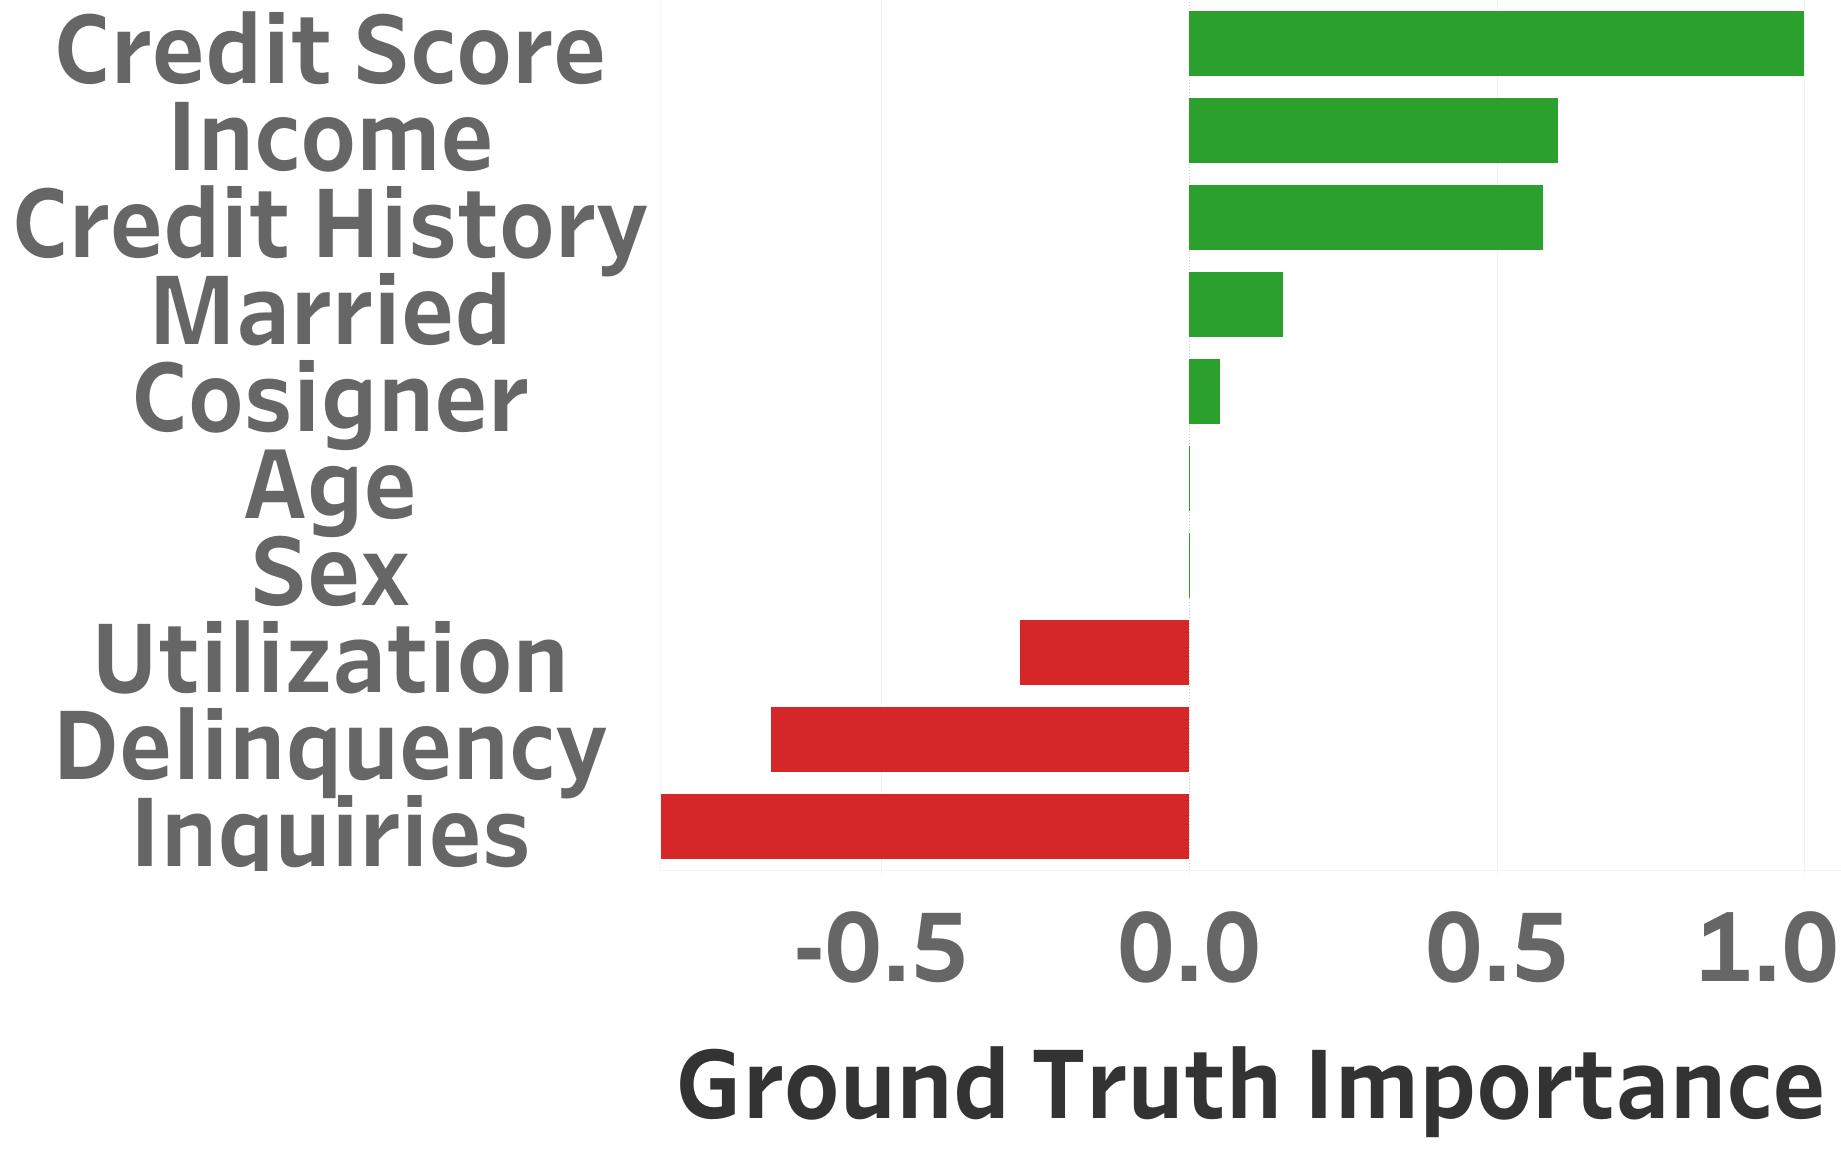
\includegraphics[width=\linewidth]{Figs/g_ex.png}
    \end{minipage}} & \multicolumn{3}{c}{\begin{minipage}{.45\textwidth}
      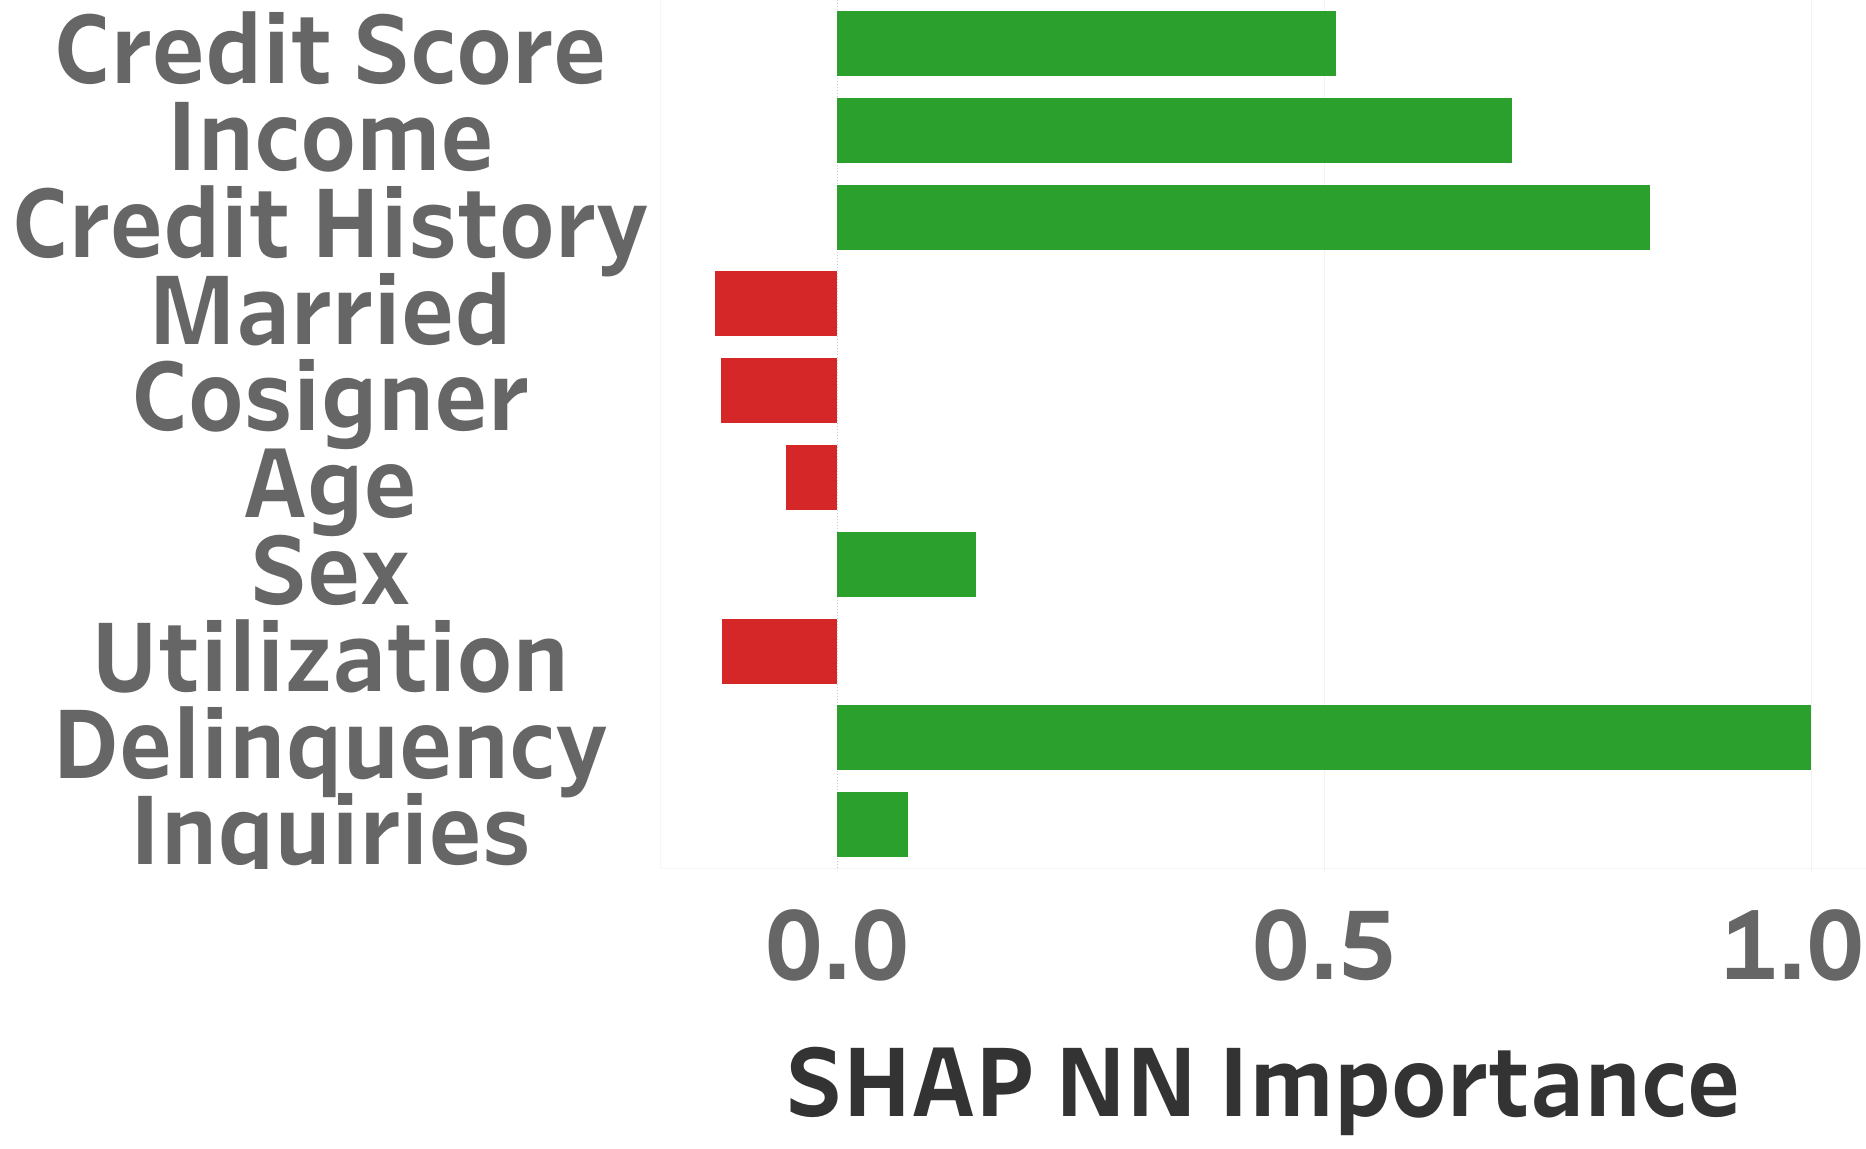
\includegraphics[width=\linewidth]{Figures/shap_mlp_ex.png}
    \end{minipage}}  %& \multicolumn{3}{c}{\begin{minipage}{.3\textwidth}
     % 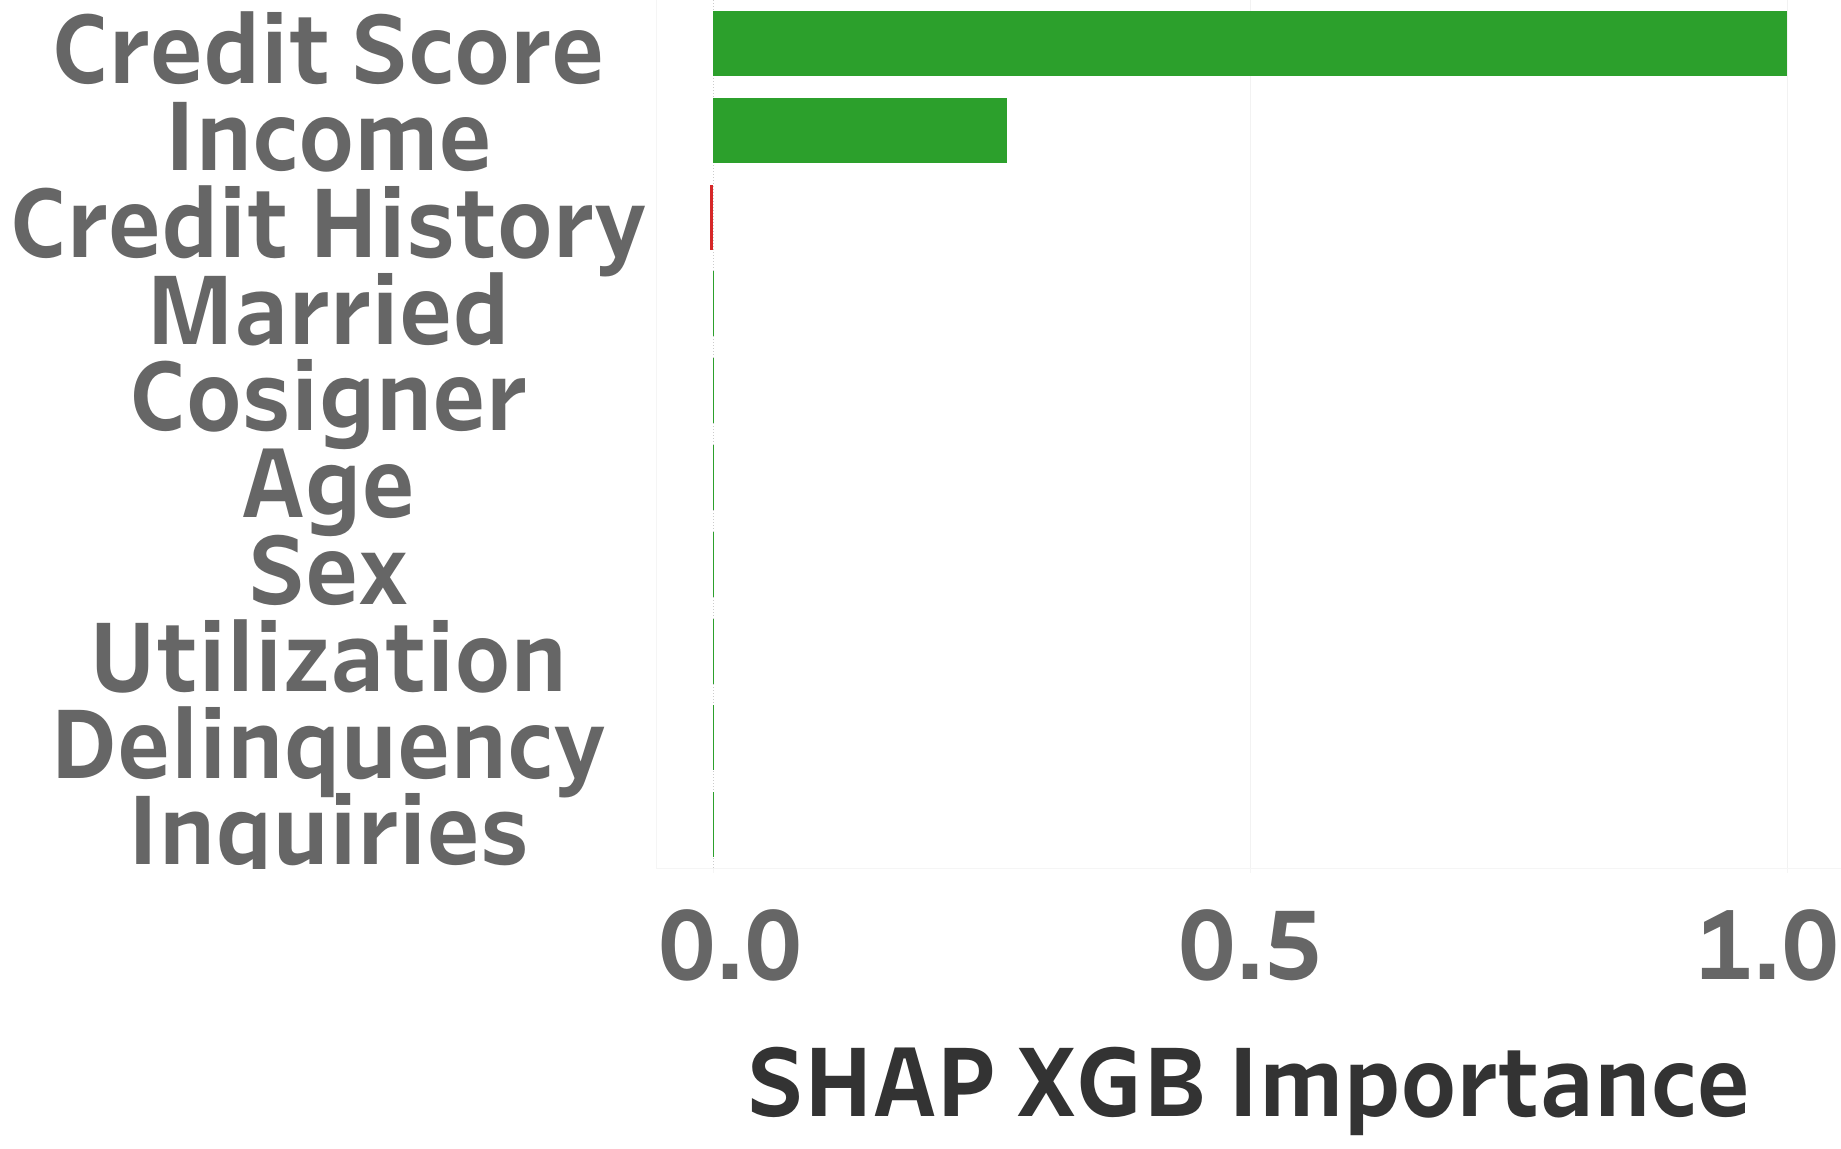
\includegraphics[width=\linewidth]{Figs/shap_xgb_ex.png}
    %\end{minipage}} 
    \tabularnewline \midrule
\end{tcolorbox}
% \noindent\begin{minipage}{\textwidth}
% \captionof{figure}{Ground truth feature importance along with qualitatively different explanations for John obtained by SHAP. %In the second pipeline, SHAP is used to explain an XGBoost model with similar performance. Feature importances are illustrated using diverging bar charts.
% }\label{box}
% \end{minipage}
\vspace{-4mm}
              \caption{Ground truth and SHAP explanation for John}
              \label{box}
            \end{subfigure}
        \caption{John's demographics along with a plot of the SHAP values obtained by explaining $\mathcal{M}$'s prediction for John, compared against the ground truth from $\mathcal{G}$.}
        \label{fig:shap_ex_full}
        \end{figure}


 Following how post hoc explanations are interpreted in the literature, we now inspect the $e_\text{SHAP}(x_j)$ coefficients to try to infer some information about the marginal effect of each feature. First, we can use the sign of the coefficients to infer the directionality of the impact of features. For example, we may deduce that the negative SHAP coefficient of ``Married'' in Figure \ref{box} implies that if an applicant is married, the likelihood of loan approval decreases. We could use this proposition to infer that being married has a negative relationship with loan approval in reality. Second, we can use SHAP coefficients to make inferences about the relative importance of features. For example, ``Delinquency" has the largest positive impact, while ``Married" has the largest negative impact. Finally, we can use the magnitudes of the features to identify the most influential features. In this case, ``Delinquency," ``Credit History" and ``Income" are the three most important features. 

%We inspect the quality of the SHAP explanations by comparing the $e_\text{SHAP}(x_j)$ with the $\beta_j$ because  the $\beta_j$ govern the ground truth relationship between explanatory variables and the target variable. Feature importance according to $\mathcal{G}$ and SHAP are shown in the left and right plots (Pipeline: $\mM=$NN) in Figure \ref{box} respectively.

Unfortunately, the above model explanation leads to significant data misinterpretation -- the  explanation differs significantly from the true marginal effects in every way, not just in value, but even in sign and relative importance. For example, the most important feature (largest $\beta_j$) should be ``Credit Score'' but SHAP suggests ``Delinquency'' is the most important. In addition, being married should have a positive impact on getting a loan application approved, and yet SHAP implies that the impact is negative. %This example underscores the inherent pitfalls in relying on post hoc explanations to deduce the true marginal effects in the data, offering a stark illustration of how their application can yield misleading interpretations. 

%Beyond the evident misalignment, the inconsistency of the explanations further compounds the problem. Repeating the pipeline with alternative selections for $\mathcal{M}$ while maintaining all other parameters constant yields divergent SHAP explanations, as shown in the right plot of Figure \ref{fig:shap_ex}. These explanations vary greatly; the only point of agreement is that ``Credit Score" and ``Income" are important features assigned positive Shapley values. 
The demonstration of the \textit{misalignment} %and \textit{inconsistency} 
of post hoc explainers  motivates the main thrust of this paper. That is, we want to find out why post hoc explainers are misaligned, what resulting harm could be done to researchers using such explainers, and what mitigation strategies could be employed for recourse. 
The ensuing sections will explicate the risks associated with employing post hoc explanations to make inferences about marginal effects. We aim to provide a detailed theoretical foundation for their limitations and a thorough critique backed by empirical evidence, revealing the dangers of this approach.
%   We see from the difference in relative magnitudes of the coefficients from $e(x_j)$ in Figure \ref{fig:shap_ex} and the ground truth in Equation \ref{eqn:gt} that the explanation for John's approval is unfaithful.


%\subsection{Inconsistency Across Pipelines}
    % We simulate this scenario and show the results obtained by the two researchers in \ref{box}. We also compare the LIME explanations they receive with the ground truth. The plots at the bottom left, bottom middle, and bottom right show the importance of each feature. The features are vertically ordered from most to least important to $\mathcal{G}$. Feature importance values for the NN and XGBoost models come from LIME's explanation of the models' decisions to approve John. They are max-normalized. The feature importance values for the ground truth are represented as the max-normalized coefficients of $\mathcal{G}$ from Equation \ref{eqn:gt}. We use max-normalization because the feature importance values of LIME and the coefficients of $\mathcal{G}$ occur on different scales. In the left and middle panels, the feature importance plots being visualized are for the ground truth and NN from the previous section. For the right panel, we trained an XGBoost model with 3 estimators that achieves about an $85\%$ test set accuracy. Although they had similar accuracies, the NN and XGBoost models may have captured different correlations in the data because the explanations of the NN and XGBoost models were quite different from each other. The explanations of both black boxes were unfaithful and both had distinct errors (otherwise all three feature importance plots would look nearly identical). To see this, note that in pipeline 1 credit inquiries are implied to be the most important even though credit score is actually the most important. Also note that although credit score was correctly identified as the most important in pipeline 2, all the other features, except income, were incorrectly implied to be negligible. The explanations of pipelines 1 and 2 are also contradictory in that in pipeline 1 being male (sex$=1$) has a positive impact on approval chances while in pipeline 2 being male has a negative impact. 
     





\section{Misalignment of Post Hoc Explanations}
\label{sec:misalignment}
  In this section, we study the research problem in more depth. We first describe how we evaluate explanations in Section \ref{sec:evaluating_faithfulness} and show the generality of the problem of misalignment in Section \ref{sec:pervasive}. 
  Then, in Section \ref{sec:causes_of_misalignment}, we identify properties of the data $\mD$, the model $\mM$, and the explainer $\mE$ used in a pipeline that lead to misaligned explanations and demonstrate how those individually affect the explanation.  %%The experiments in this section all use our running example of explaining loan application decisions, where the ground truth model is a linear model. 

\subsection{New Metrics for Assessing Post hoc Explanations}
   \label{sec:evaluating_faithfulness}
  Both SHAP and LIME provide a feature importance measurement for each feature $j$, which we denote by $e_\mE(x^{(i)}_j)$, where $\mE$ represents the explainer.
   Our goal is to investigate whether $e_\mE(x^{(i)}_j)$ can be used to provide correct information about the marginal effect of feature $j$. To this end, we propose three new metrics that capture different aspects of explanations, each motivated by practical use cases of explanations from the literature: sign, importance ranking, and relevance. 
     
     First, we give a more detailed definition of the true marginal effects $\boldsymbol{\beta}$ so that our estimand is clear. Our characterization of $\boldsymbol{\beta}$ captures both the correlative effect that each explanatory variable has on the response variable individually as well as any effects that one variable can have on the target through other variables that depend on it. This is accomplished by considering two cases in our definition. If a feature $X_j$ depends on any other feature, we define $\beta_j$ to be the total derivative $\dv{Y}{X_j}$. Otherwise, we define $\beta_j = \pdv{Y}{X_j}$. Therefore, for linear models, the marginal effects equal the model coefficients.



         
         % The metrics we propose are motivated by how the post hoc feature importances are used in business research.
          We design three metrics to evaluate data-alignment  considering the practical use case of the explanations. Researchers using SHAP and LIME typically use the feature importance values in three main ways: 1) inspect the sign of the feature importance values to identify how the features impact the outcome they are interested in %For example, in \citep{park2024extracting} says that the quad-core feature of smartphones having a negative SHAP value also indicates a negative effect on consumer choices. 
         2)  identify the relative importance of features %This type of analysis is exemplified in \citep{zhang2023explainable}, which advocates for managers to use the top most important features from the ranking they obtained via SHAP as early indicators of financial risk in manufacturing companies. 
         and 3) identify the most influential features. %cite kovvuri
    %To capture how well SHAP and LIME can do these things, we use three metrics. 

    Therefore, we define the first metric, termed \textbf{directionality}, to measure whether post hoc explainers can at least identify the correct \textit{sign} of a feature's influence on the outcome. It evaluates an explanation only qualitatively. We calculate directionality by determining the percentage of instances where the sign of $e_\mE(x^{(i)}_j)$ matches that of $\beta_j$ for feature $j$ across $M$ instances in the test set. %However, when $\beta_j$ is sufficiently small, checking the sign agreement would be too strict. Thus, we relax the definition and instead check if $\mid e_\mE(x^{(i)}_j)\mid $ is also very small relative to the largest feature importance value $\max_{j^\prime} \mid e_\mE(x^{(i)}_{j^\prime}) \mid $.
    % Given the ground truth $\beta_j$ and feature importance values $e_\mE(x^{(i)}_j)$ from an explainer, we denote the accuracy for the $j^{\text{th}}$ feature as follows. 
    % Note that this definition is  made in reference to the entire test set $\{x^{(i)}\}_{i=1}^n$ but considers only one feature index $j$.  %The notation $\hat{\beta}^{(i)}$ represents a feature importance vector for the $i^{\text{th}}$ test set instance. 
    \begin{equation}
        \label{eq:acc}
        \texttt{directionality}(\{e_\mE(x^{(i)}_j)\}_{i=1}^M,\beta_j) = \frac{1}{M} \sum_{i=1}^M s_j( e_\mE(x^{(i)}_j),\beta_j)
    \end{equation}
    where 
    \begin{equation*}
        s_j(e_\mE(x^{(i)}_j),\beta_j) = \begin{cases*}
                    \mathbf{1}_{\mathbb{R}^+}(\beta_j \cdot e_\mE(x^{(i)}_j)) & if  $\mid \beta_j\mid > \epsilon_1$  \\
                     \mathbf{1}_{(0,\epsilon_2)}\left(\frac{\mid e_\mE(x^{(i)}_j)\mid }{\max_{j'} \mid e_\mE(x^{(i)}_{j'})\mid}\right) & otherwise
                 \end{cases*}
    \end{equation*}
    Here $\mathbf{1}_S(z)$ is an indicator function that returns 1 if $z$ is in the set $S$ and outputs 0 otherwise. $s_j(e_\mE(x^{(i)}_j),\beta_j)$ is designed to facilitate a relaxed version of accuracy by checking if $\beta_j$ and $e_\mE(x^{(i)}_j)$ have the same sign only when $\beta_j$ is not very small, i.e., larger than some $\epsilon_1> 0$ in magnitude. When $\beta_j$ is small, $s_j$ instead checks if $e_\mE(x^{(i)}_j)$ is small relative to the other $e_\mE(x^{(i)}_{j^{\prime}})$, where $j^\prime \neq j$. In particular, the ratio of $\mid e_\mE(x^{(i)}_j)\mid $ and $\max_j^\prime \mid e_\mE(x^{(i)}_{j^\prime})\mid$ should be small. We check this using a variable threshold $\epsilon_2$. In our experiments, we use $\epsilon_1=1e-2$ and $\epsilon_2=1e-2$. This definition uses a relaxed conception of accuracy because, for example, if a ground truth marginal effect is 0.001 and the explanation returns -0.001, we would consider the explanation to correct, even if the signs do not agree, because both correctly identify that the feature has a very small impact on $Y$ relative to the most important feature.
    
      The second metric, \textbf{concordance}, measures how accurately the explanations recover the \textit{relative importance} of features compared to the ground truth ranking induced by $\boldsymbol{\beta}$. Given the $e_\mathcal{E}(x^{(i)}_j)$, we rank the features from least to most important and calculate the \emph{Spearman Rank Correlation} \citep{spearman1904proof} between this ranking and a ranking of the $\beta_j$. While the directionality metric is computed using the entire test set per feature, concordance is computed per instance using all features.

    % The Spearman rank correlation is defined as follows. 
    \begin{equation}
       \texttt{concordance}(e_\mE(\mathbf{x}^{(i)}),\boldsymbol{\beta}) = 1 - \frac{6\sum_{j=1}^D (\text{rank}(\beta_j) - \text{rank}(e_\mE(x^{(i)}_j)))^2}{D(D^2-1)},
    \end{equation}
    Above, $D$ is the number of features and $\text{rank}(\beta_j)$ and $\text{rank}(e_\mE(x^{(i)}_j))$ denote the rank of the $j^{\text{th}}$ feature according to the coefficients of $\boldsymbol{\beta}$ and explanations $e_\mE(\mathbf{x}^{(i)})$, respectively. If an explainer's rankings are 100\% correct, then this correlation should be 1. Any value less than 1 indicates an error in the rankings (which can lead users to misinterpret the importance of some features).
    
Third, motivated by the fact that researchers may only be interested in identifying a small set of features that have the highest impact, we define the third metric, \textbf{relevance}, based on the ranking of features. Our metric, denoted $\text{relevance}_k$, measures how many of the top $k$ most important features according to $\mathcal{E}$  are among the top $k$ largest  marginal effects, both in magnitude. Denote by $I_k^+(e_\mE(\mathbf{x}^{(i)}))$ and $I_k^+(\boldsymbol{\beta})$  the set of feature indices among the top $k$ most highly ranked according to $e_\mE(\mathbf{x}^{(i)})$ and $\boldsymbol{\beta}$, respectively. Then we define 
    \begin{equation}
        \texttt{relevance}_k(e_\mE(\mathbf{x}^{(i)}), \boldsymbol{\beta}) = \frac{\mid I_k^+(\boldsymbol{\beta}) \cap I_k^+(e_\mE(\mathbf{x}^{(i)}))\mid}{k}.
    \end{equation}
     Like the concordance metric, $\text{relevance}_k$ is also computed at the instance level. 
    In our experiments, we compute $\text{relevance}_k$ for each $k$ and plot the means and standard errors over $M$ instances. $\text{relevance}_k(e_\mE(\mathbf{x}^{(i)}), \boldsymbol{\beta})$ represents the recall for the identification of features among the top-$k$ largest marginal effects according to $\mathcal{E}$.       
    
   
        



                    \begin{figure}[ht!]
            \centering
            \begin{subfigure}[t]{.28\textwidth}
              \centering
              \captionsetup{justification=centering}
                  \raisebox{.2cm}{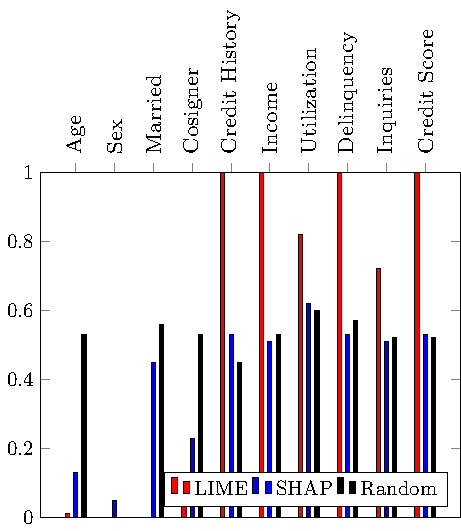
\includegraphics[width=\textwidth]{Figures/sec4_1-figure0.pdf}}%{Figures/lime_shap_Spearman_magnitude.png}
              \caption{Directionality}%Spearman rank correlations of feature importance magnitudes from SHAP and LIME against the true ranking from $\mathcal{G}$. }
               \label{fig:lime_shap_sign_accs}
            \end{subfigure}%
            \hspace{1cm}%\hfill
            \begin{subfigure}[t]{.28\textwidth}
              \centering
               \captionsetup{justification=centering}
              \raisebox{.05cm}{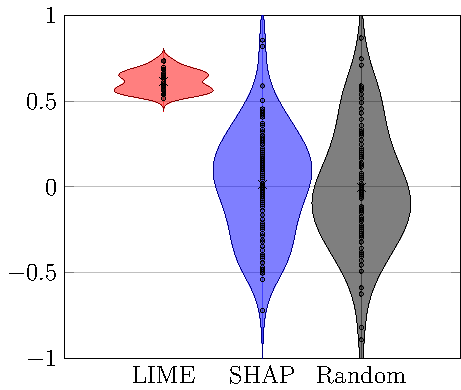
\includegraphics[width=\textwidth]{Figures/sec4_1-figure1.pdf}}%{Figures/lime_shap_Spearman_signed.png}
              \caption{Concordance}%Spearman rank correlations of signed feature importance from SHAP and LIME against the true ranking from $\mathcal{G}$.}
               \label{fig:lime_shap_Spearman_signed}
            \end{subfigure}
            \hspace{1cm}%\hfill
            \begin{subfigure}[t]{.28\textwidth}
              \centering
               \captionsetup{justification=centering}
            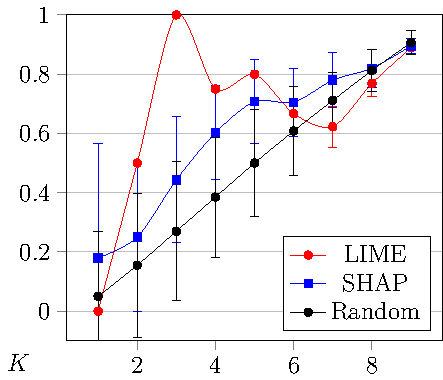
\includegraphics[width=\textwidth]{Figures/sec4_1-figure2.pdf}%
            \caption{Relevance}%The average and standard error of recall of SHAP and LIME when attempting to capture the top K most important features to $\mathcal{G}$ when explaining $\mathcal{M}$, for varied $K=1,2,3,...$ number of features.}
            \label{fig:avg_recall}
            \end{subfigure}
            \caption{Illustration of the three aspects of data-alignment evaluation. For plot (c) each point in the line plot represents a mean relevance for a given $k$. The error bars represent the standard error. The total number of features is 10.}
           \label{fig:beta_alignment}
        \end{figure}    
 
  We call the evaluation of the directionality, concordance, and relevance the evaluation of \textbf{data-alignment}. We evaluate the data-alignment
 for SHAP and LIME on $M=100$ applicants randomly selected from the test set and report the results in Figure \ref{fig:beta_alignment}. 
 We find that neither SHAP nor LIME achieves satisfying results on any of the three dimensions. Most notably, in spite of the fact that SHAP is strongly favored over LIME by researchers (91\% vs 14\% from the papers we surveyed), SHAP performs significantly worse than LIME in all three dimensions. \textbf{SHAP cannot even identify the correct directionality of the features}, let alone the concordance and relevance. To have a better understanding of the data-alignment of SHAP, we also simulate a \emph{random} explainer that randomly draws its feature importance values $e_\text{random}(x^{(i)}_j)$ from a standard normal distribution for each $j$ and $i$. We find that \emph{SHAP explanations do not have better data-alignment than random explanations  with respect to directionality and concordance.}         


\subsection{Pervasiveness of Data-Misalignment - a Large Scale Evaluation}
    \label{sec:pervasive}
    So far, we have only used one simulated dataset to demonstrate the misalignment of SHAP and LIME explanations. To study how pervasive the issue is, % We show that data-misalignment is a general property of SHAP and LIME. In doing this, the implications of Section \ref{sec:causes_of_misalignment} are corroborated and the scope of their validity is widened. We do this by evaluating the data-alignment of 
    we evaluate the SHAP and LIME explanations using 100 simulated datasets.
    
    Our 100 synthetic datasets have randomly selected numbers of features between 3 and 100, and randomly selected numbers of rows between 100 and 10000. The features are i.i.d. according to $\mathcal{N}(0,5)$. The target of each dataset is binary and is produced using randomly generated linear decision boundaries. To generate the linear decision boundaries, we randomly generated integer coefficients between -10 and 10 and  constructed the linear decision functions with those coefficients. Each dataset used one of these functions to generate labels for each sample.  %We vary the amount of label noise in each dataset by fixing a probability $p \in [0,.1]$ before generating the dataset and then flipping each label with probability $p$.
    We split each dataset into 80\% training data and 20\% testing data.  The test set accuracies of all models fall between $.82$ and $.99$. It is important to note that as these datasets all have i.i.d. normal features and there is no noise in the target column, this experiment uses practically ideal conditions for the training and subsequent explanation of ML models.


        Since the number of features differs between the datasets, we report the results for our three metrics in the following fashion, conditioned on the number of features. %For directionality, for each $d$, we report the mean directionality for the actual most important feature over 100 test set instances from the datasets with dimension $d$. 
        For each dataset, we compute feature-wise mean directionality, mean concordance over $M$ test instances, and mean relevance for $k=3$ over $M$ test instances. This gives us a single measurement of each metric for each dataset. We partition the results for each dataset based on which of the five equal width bins of [1,100] the associated $D$ falls into. Finally, we report the means within each bin for each metric in Figure \ref{fig:lime_shap_vary_d}.  %We report the information similarly for the number of rows $n$ rather than $d$ below.   

    
    Our experimental results imply that SHAP and LIME explanations do not in general produce faithful information about marginal effects, and also that explanation quality further decreases as the number of features increases. Indeed, Figure \ref{fig:lime_shap_vary_d} shows that, generally when $D$ exceeds $20$, mean directionality for SHAP is actually under $.5$ which is worse than random guessing. LIME's mean directionality for $D> 20$ is not much better as it is still generally close to $.5$. This is an alarming sign because the two most popular post hoc explainers can not even get a correct qualitative estimation of the true marginal effect --- even the sign is wrong! In addition, both the mean concordance and mean relevance for $k=3$ are low especially when there are more than 20 features. It is also notable that the more features there are, the more challenging it is for the two explainers to correctly identify the contributions of each feature, as there exist more possible mappings from the input to the output that could be different from that of $\mG$ and there is no control over which one $\mM$ uses. Overall, we noticed a negative association between $D$ and each of our metrics. 

      \begin{figure}[ht!]
      \captionsetup{labelfont=footnotesize,textfont=footnotesize}
      \captionsetup[subfloat]{labelfont=scriptsize,textfont=scriptsize,justification=centering}
      \centering
      \subfloat[Mean Directionality]{%
        \hspace{0mm}
        \raisebox{0cm}{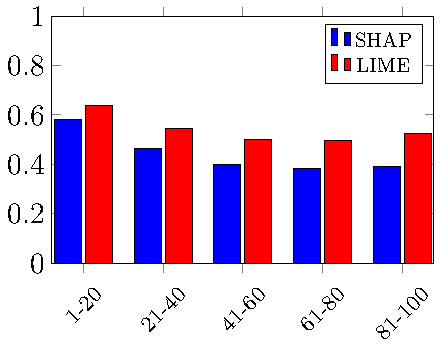
\includegraphics[width=0.28\textwidth]{Figures/lime_shap_synthetic-figure0.pdf}\quad}%
        \label{fig:shap_vary_d_accs}%
      }\hspace{1cm}%\hfill
      \subfloat[Concordance]{%
        \raisebox{0cm}{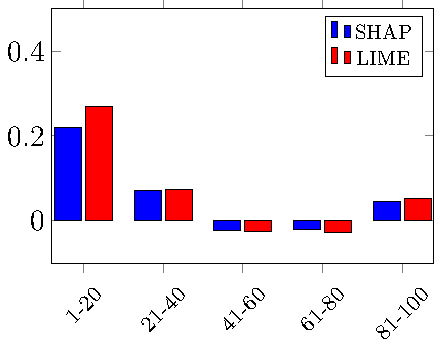
\includegraphics[width=0.28\textwidth]{Figures/lime_shap_synthetic-figure1.pdf}}%
        \label{fig:shap_vary_d_spearmans}%
      }\hspace{1cm}%\hfill
      \subfloat[Top-3 Relevance]{%
        \raisebox{0cm}{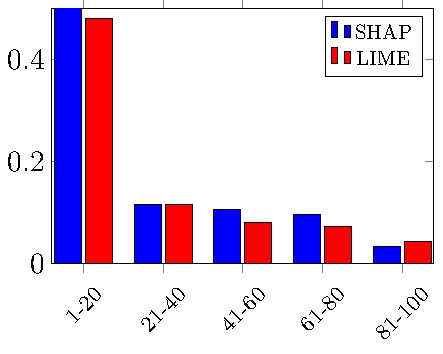
\includegraphics[width=0.28\textwidth]{Figures/lime_shap_synthetic-figure2.pdf}}%
        \label{fig:shap_vary_d_rels}%
      }\\
      % % \subfloat[LIME Top-1 Directionality]{%
      % %   \raisebox{0cm}{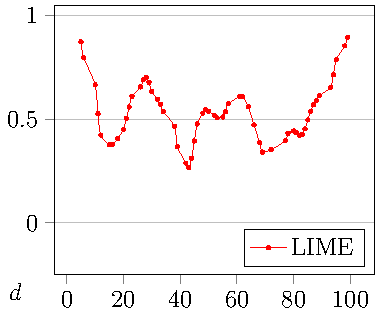
\includegraphics[width=.2\textwidth]{Figs/synthetic-figure1.pdf}}%
      % %   \label{fig:lime_vary_d_accs}%
      % % }\hspace{.5cm}%\hfill
      % \subfloat[LIME Mean Directionality]{%
      %   \hspace{0mm}
      %   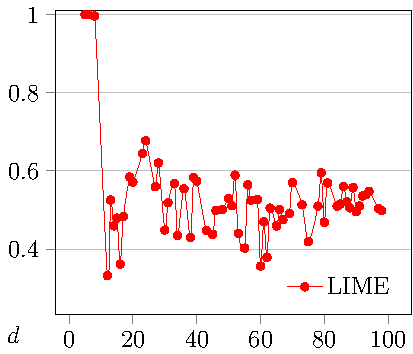
\includegraphics[width=0.178125\textwidth]{SynthFigs/meanacclime-figure0.pdf}\quad%
      %   \label{fig:lime_vary_d_spearmans}%
      % }\hspace{1cm}%\hfill
      % \subfloat[LIME Concordance]{%
      %   \hspace{0mm}
      %   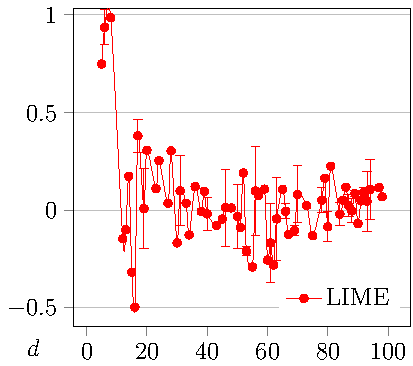
\includegraphics[width=0.178125\textwidth]{SynthFigs/conclime-figure0.pdf}%
      %   \label{fig:lime_vary_d_accs}%
      % }\hspace{1cm}%\hfill
      % \subfloat[LIME Top-3 Relevance]{%
      %   \hspace{0mm}
      %   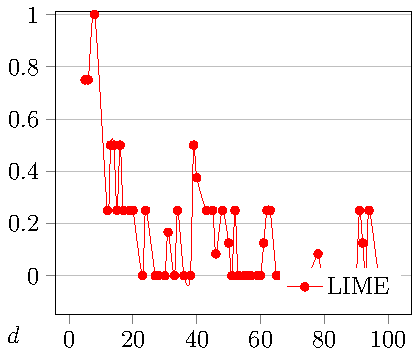
\includegraphics[width=0.178125\textwidth]{SynthFigs/rellime-figure0.pdf}%
      %   \label{fig:lime_vary_d_spearmans}%
      % }\\
      \caption{Relationship of number of features $D$ with feature-wise mean directionality, concordance, and relevance for $k=3$}
      \label{fig:lime_shap_vary_d}
    \end{figure}




  
    \subsection{Contributing Factors to  Misalignment}
        \label{sec:causes_of_misalignment}
        We investigate factors in the pipeline that contribute to misalignment. Our aim is to provide both theoretical and empirical evidence for why post hoc explanations should not be used to make inferences about the actual input-output relationships underlying data. Our investigation will examine both stages of the explanation pipeline (the prediction stage and the explanation stage). % We first investigate SHAP and LIME in the explanation stage to show how their inherent model design contributes to misalignment. 
        We work under the assumptions that domain knowledge about the data generation process is unavailable. Due to the space limit, we show our experiments on one dataset. However, as robustness check, we repeat each experiment again on a different dataset in the Appendix. %The experiments in this section involve first training an ML model $\mathcal{M}$ and then building an explainer model $\mathcal{E}$ to produce explanations. % training data to build a machine learning model and then and explanations of predictions of those NNs on instances from the remaining 20\% of data reserved as a test set.


    \subsubsection{Explainers May Inherently Be Misaligned}
    \label{sec:theoretical_considerations}
   We first investigate how explainers themselves contribute to misalignment by deriving and analyzing equations for their explanations of linear models. To exclude other factors in the explanation pipeline, we assume here that we have access to the ground truth model $\mathcal{G}$ and that SHAP and LIME are directly applied to explaining $\mathcal{G}$ rather than $\mathcal{M}$. Thus, the explanations are solely based on the explanation stage. We suppose that $\mathcal{G}$ is a simple linear function of $D$ features and SHAP and LIME explain the output of $\mathcal{G}$ at a point $\boldsymbol{\xi}$, that is, $\mathcal{G} = \boldsymbol{\beta}^T \mathbf{x}$ where $\mathbf{x} \sim \mathcal{N}(\mathbf{0}_D,\bI_{D\times D})$ and $\boldsymbol{\xi}$ is a realization of $\mathbf{x}$. Below, we derive mathematical representations of SHAP and LIME explanations, and investigate their relationships with the marginal effects $\boldsymbol{\beta}$.

         \paragraph{$e_{\text{SHAP}}$ when Explaining a Linear Model}
              %SHAP does \emph{not} recover $\boldsymbol{\beta}$ and should not be relied upon for this purpose. 
              The importance of the $j^{th}$ feature of the $i^{th}$ data sample $\xi^{(i)}_j$ in a SHAP explanation is the Shapley value for that feature in that sample. The Shapley value reduces to the following expression when SHAP is used to explain a linear model according to \cite{StrumbeljErik2014Epma,lundberg17shap}. 
             \begin{equation}
                \label{eqn:shap_gt}
                e_\text{SHAP}(\mathbf{x}^{(i)}_j) = \beta_j (\xi^{(i)}_j - \bar{x}_j).
             \end{equation}

            
The SHAP explanations outlined by Equation \ref{eqn:shap_gt} exhibit several undesirable properties that can limit their practical application. For example, when $\boldsymbol{\xi}=\bar{\mathbf{x}}$, the SHAP values $e_\text{SHAP}$ reduce to 0, leading to all features being deemed unimportant. Moreover, Shapley values generally cannot be used to infer the signs of the marginal effects because when $\xi^{(i)}_j - \bar{x}_j$ is negative, the signs of $e_{\text{SHAP}}(\xi^{(i)}_j)$ and $\beta_j$ are opposite. Another consequence of Equation (\ref{eqn:shap_gt})  is that the expected SHAP values average to zero, rendering them generally uninformative about the marginal effects. Some authors address this in their search for global feature importance by instead considering empirical averages of absolute SHAP values \citep{lenaers23rent,maeng23vr,guenther2023useful}. However, this comes at the cost of losing information about the directionality of a feature's impact.

             Following Equation (\ref{eqn:shap_gt}), we propose to mitigate SHAP's inherent misalignment for linear models by using what we will refer to as \emph{normalized SHAP values}: $e_{\text{SHAP}}(\xi^{(i)}_j) / (x^{(i)}_j - \bar{x}_j)$. Although this is a straightforward adjustment that can be made in order to approximate the marginal effects using SHAP, we are not aware of its use in prior literature.  Our empirical evaluation of these normalized Shapley values, which includes recalculating directionality, concordance, and comparison with traditional SHAP results (illustrated in Figures \ref{fig:shap_dividex_corr}), suggests significant improvements.
             
             Normalized SHAP values frequently exhibit correct sign alignment and generate feature rankings more concordant with the ground truth. Directionality for features related to ``Credit Score" improved remarkably, as shown in Figure \ref{fig:shap_dividex_accs}. However, directionality for the features related to cosigner access (``Married" and ``Cosigner") decreased. The improvements to feature rankings are evident from Figures \ref{fig:shap_dividex_spearmans} and \ref{fig:shap_dividex_recalls}; we can see that mean concordance rose from near 0 to about .6 and relevance was improved substantially for $k=2,3,4,5$. Normalizing SHAP values evidently gives an advantage.
             
            
             Given the evident effectiveness of the SHAP normalization scheme and our evidence that unmodified SHAP explanations are theoretically  data-misaligned, \textbf{we will adopt this normalization approach for all subsequent experiments in this paper}. This is vital as we explore the impacts of $\mathcal{M}$'s predictive performance and feature independence in subsequent sections (\ref{sec:role_of_predictive_power} and \ref{sec:role_of_correlation}). %For example, we will use it in the following subsections on the roles of $\mathcal{M}$'s predictive performance and feature independence (\ref{sec:role_of_predictive_power} and \ref{sec:role_of_correlation}). We wish to show that increasing the predictive performance of $\mathcal{M}$ and using independent training data features may increase data-alignment, so the normalization scheme is necessary because otherwise SHAP's explanations are similar to random ones and thus will be unaffected by external effects. 
           \begin{figure}[ht!]
            \centering
            \begin{subfigure}[t]{.28\textwidth}
              \centering
              \captionsetup{justification=centering}
                  \raisebox{.2cm}{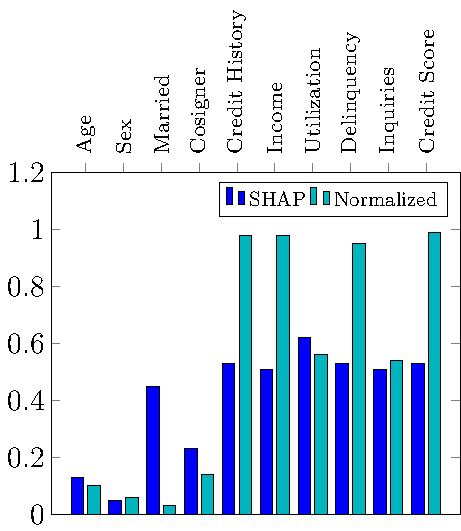
\includegraphics[width=\textwidth]{Figures/sec4_1_dividex-figure0.pdf}}%{Figures/lime_shap_Spearman_magnitude.png}

              \caption{Directionality}%Spearman rank correlations of feature importance magnitudes from SHAP and LIME against the true ranking from $\mathcal{G}$. }
               \label{fig:shap_dividex_accs}
            \end{subfigure}%
            \hspace{1cm}%\hfill
            \begin{subfigure}[t]{.28\textwidth}
              \centering
               \captionsetup{justification=centering}
              \raisebox{.05cm}{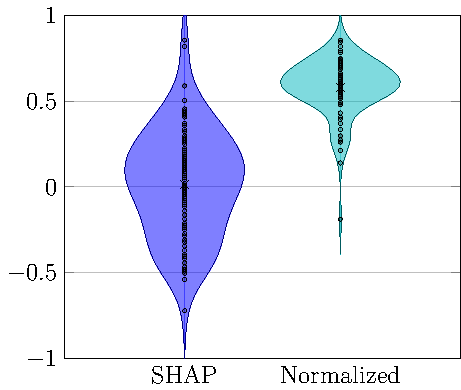
\includegraphics[width=\textwidth]{Figures/sec4_1_dividex-figure1.pdf}}%{Figures/lime_shap_Spearman_signed.png}
              \caption{Concordance}%Spearman rank correlations of signed feature importance from SHAP and LIME against the true ranking from $\mathcal{G}$.}
               \label{fig:shap_dividex_spearmans}
            \end{subfigure}
            \hspace{1cm}%\hfill
            \begin{subfigure}[t]{.28\textwidth}
              \centering
               \captionsetup{justification=centering}
            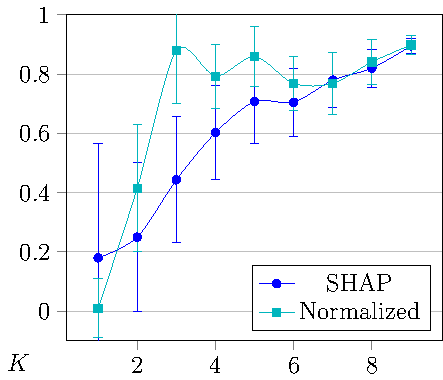
\includegraphics[width=\textwidth]{Figures/sec4_1_dividex-figure2.pdf}%
            \caption{Relevance}%The average and standard error of recall of SHAP and LIME when attempting to capture the top K most important features to $\mathcal{G}$ when explaining $\mathcal{M}$, for varied $K=1,2,3,...$ number of features.}
            \label{fig:shap_dividex_recalls}
            \end{subfigure}
            \caption{Comparison of SHAP explanations without and with SHAP value normalization}
           \label{fig:shap_dividex_corr}
        \end{figure}   
        \paragraph{$e_{\text{LIME}}$ when Explaining a Linear Model}
            \label{sec:lime_linear_case}
             %In this section we we will show that there are conditions when the LIME coefficients have the property $e(x_j)\simeq \beta$ and use this fact to justify that  $e(x_j)$ can be evaluated with respect to the ground truth $\boldsymbol{\beta}$. Those conditions are discussed in the next paragraph. 
             
             %%LIME works by sampling data points around a given instance, then using these samples to train a weighted linear model as a local surrogate model that approximates the predictions of the original complex model in the vicinity of the instance. The local surrogate model is trained as a weighted ridge regressor. To obtain interpretable and sparse explanations, LIME discretizes numerical features and includes a regularization component to promote sparsity in the local surrogate models it creates. This regularization helps in selecting a subset of features that are most influential for predictions near the instance being explained, thus ensuring that the explanations are both interpretable and concise. 
             Recall from Section \ref{sec:related_work} that LIME's explanation model is a weighted ridge regressor trained on discretized data sampled around the instance being explained. By discretizating numerical features and using weighted ridge regression (rather than standard least squares), the possibility of LIME's data-alignment is compromised. The use of discretized features in LIME's ridge regression model can eliminate critical information about the model being explained. Additionally, the sparsity penalty which is used in ridge regression may zero out coefficients for features that actually have a non-zero marginal effect, distorting the picture one may obtain of the marginal effects. Also, employing weighted ridge regression introduces a weight matrix that further skews the estimation of marginal effects. This distortion can be observed in the closed-form solution of the weighted ridge regression, indicating potential limitations in LIME's ability to provide accurate estimates under certain conditions.
             
              Having identified the aforementioned properties of LIME's regression design as contributors to its lack of data-alignment, we derive conditions under which LIME would be data-aligned. We begin this effort by analyzing the large sample behavior of LIME coefficients in an idealized scenario where LIME does not use discretization and the model being explained is a linear function of i.i.d. normal features. Under such idealized assumptions, our Theorem \ref{thm:lime_thm} below shows that LIME's coefficients converge to $\boldsymbol{\beta}$ as the number of samples $N$ tends to $\infty$. %Our Corollary 1 analyzes the closed form for the coefficients in order to ascertain the conditions for LIME's alignment in this idealized scenario. 
            \begin{theorem}
                \label{thm:lime_thm}
                Suppose $f:\mathbb{R}^D\rightarrow \mathbb{R}$ that maps $\mathbf{x} \mapsto \boldsymbol{\beta}^T \mathbf{x}$ is explained at a sample $\boldsymbol{\xi}$ drawn from $\mathcal{N}(\mathbf{0}_D, \bI_{D\times D})$ with LIME. Suppose further that LIME does not discretize features and samples i.i.d. data points $\mathbf{x}^{(1)},\ldots,\mathbf{x}^{(N)}$ from $ \mathcal{N}(\boldsymbol{\xi}, \bI_{D\times D})$ for its regression.
                 Then, in the large sample limit, LIME recovers $\boldsymbol{\beta}$.  
            \end{theorem}

             % Although LIME does not recover $\boldsymbol{\beta}$ with its default settings, Theorem 2 shows that $e_{\text{LIME}}(\mathbf{x}^{(i)}_j)$ converges to $\boldsymbol{\beta}$ in the large $n$ limit when explaining a linear model $\boldsymbol{\beta}^T \mathbf{x}$ where the data $\mathbf{x}$ are sampled from a standard multivariate normal distribution and LIME does not discretize continuous features.
             Theorem 1 uses an application of the law of large numbers to show that, in the large sample limit of random design matrices $\mathbf{X}$, LIME recovers $\boldsymbol{\beta}$. The practical implication of this theorem is that, when using LIME, $N$ should be large.  For a non-asymptotic analysis, see the Appendix. %We also show that if $\nu$ is too small the LIME coefficients all go to $\mathbf{0}$.

            \begin{remark2}
                \label{nu_remark}
                Given a fixed number of samples $N$, the kernel bandwidth $\nu$ being too small makes each of LIME's coefficients close to $0$. $\nu$ being very large can lead to a better approximation of $\boldsymbol{\beta}$. 
            \end{remark2}

            Remark \ref{nu_remark}, which is justified by our non-asymptotic analysis, suggests that when $N$ is fixed and finite, $\nu$  should also be set to be large. Notably, \citep{garreau20theoretical} obtained these same conclusions about $\nu$ and $N$ in the case where discretization is used. Numerical experiments justifying these conclusions, as well as the proof for Theorem 1 and justification of Remark 1 can be found in the appendix. 
    \subsubsection{The Role of the Predictive Power of $\mathcal{M}$}
        \label{sec:role_of_predictive_power}
           % The goal of the explanation pipeline is to unveil the underlying $\boldsymbol{\beta}$ within the unobservable structure $\mathcal{G}$. 
           Another factor in the pipeline that has a significant impact on  explanations is the machine learning model $\mathcal{M}$ itself. 
      An explainer $\mathcal{E}$ is never directly applied to $\mathcal{G}$ because  $\mathcal{G}$ is not directly observable. Instead, $\mathcal{E}$ is applied to a model $\mathcal{M}$ constructed based on data derived from $\mathcal{G}$. Consequently, it is reasonable to infer that the fidelity of $\mathcal{M}$ with respect to $\mathcal{G}$—that is, how accurately $\mathcal{M}$ reflects the true structure of $\mathcal{G}$—significantly influences the data-alignment of explanations. This fidelity can be reflected by the predictive performance of $\mM$.  

           It is also worth mentioning that high predictive accuracy of $\mathcal{M}$ does not unequivocally confirm an accurate apprehension of $\mathcal{G}$, since factors such as multicollinearity might lead to $\mathcal{M}$ making accurate predictions without faithfully capturing the training data's underlying dynamics. Nevertheless, this nuance does not eliminate the reliability of predictive performance as an indicator of $\mathcal{M}$'s quality. Specifically, while high accuracy does not guarantee an accurate apprehension of $\mathcal{G}$, low accuracy definitively signals that $\mathcal{M}$ fails to represent $\mathcal{G}$ accurately. Therefore, predictive accuracy stands as a limited but reliable measure for assessing $\mathcal{M}$'s quality.
 
            
            We investigate the relationship between the predictive power of $\mathcal{M}$ and the alignment of explanations of $\mM$ by comparing SHAP and LIME explanations of NNs $\mathcal{M}_1$  with ROC AUC approximately equal to $0.60$ and $\mathcal{M}_3$ with AUC equal to $0.99$. We also use the NN with AUC $.93$ from Section \ref{sec:evaluating_faithfulness} as an intermediate model $\mathcal{M}_2$. When training $M_1$ and $M_3$, they start out as the same model (through random seed initialization) but are trained for sufficiently many epochs to achieve their corresponding AUCs of .6 and .93, respectively. Moreover, we follow Equation \ref{eqn:shap_gt} and normalize the SHAP values in this experiment, thereby bypassing SHAP's inherent data-misalignment and enabling us to show how increasing model AUC can aid the usage of SHAP. The results are shown in Figure \ref{fig:mlp_auc_increase} and demonstrate the positive relationship model performance has on data-alignment for both SHAP and LIME.
            
     Figure \ref{fig:mlp_auc_increase} shows that as the performance of the black box improves, the explanations become more data-aligned with respect to all three metrics. However, it should be noted that despite $\mathcal{M}_3$ achieving near perfect performance, with an AUC of $.99$, neither of the two most favored explainers were able to obtain perfect or near perfect data-alignment. They consistently struggled to identify even the fundamental qualitative relationships among variables, such as directionality. This implies that in practical scenarios, even an ML model with perfect accuracy may not enable researchers to interpret the significance—or even the direction—of feature importance in relation to the true marginal effects.  
     
     Our results here highlight a significant risk that features presumed to positively influence the outcome may, in fact, have a detrimental effect. This is because ML models are trained to produce the correct \emph{predictions}, but not necessarily the correct \emph{mapping} from the input to the predictions, i.e., how features contribute to the predictions could be different from that in the ground truth $\mathcal{G}$. In fact, there may exist many possible mappings that lead to the same or similarly good predictions, according to the Rashomon set theory \citep{semenova22rashomon}. This also explains the results in Figure \ref{fig:lime_shap_vary_d} from Section \ref{sec:pervasive}. As the number of features increases, the number of possible mappings from the input to the predictions grows. This lowers the chance that a machine learning model will capture the correct relationship. 
      Consequently, the crucial insight here is that while constructing an accurate ML model is beneficial, it \emph{does not guarantee} utility in understanding the true relationships in the data. 

        \begin{figure}[t!]
            \subfloat[SHAP Directionality]{%
                \raisebox{.2cm}{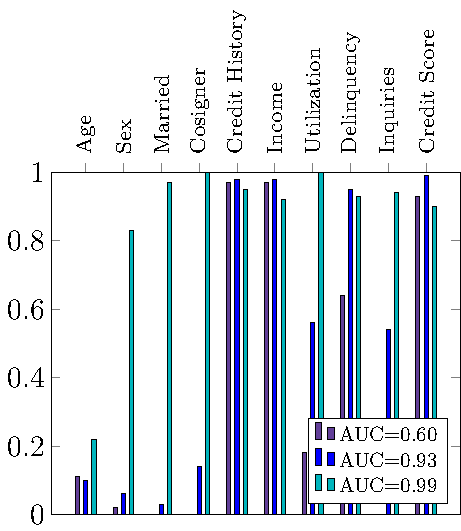
\includegraphics[width=.28\textwidth]{Figures/sec4_4_mlp_auc_shap-figure0.pdf}}%
                \label{subfig:mlp_auc_shap_sign_accs}%
            }\hspace{1cm}
            \subfloat[SHAP Concordance]{%
                 \raisebox{.05cm}{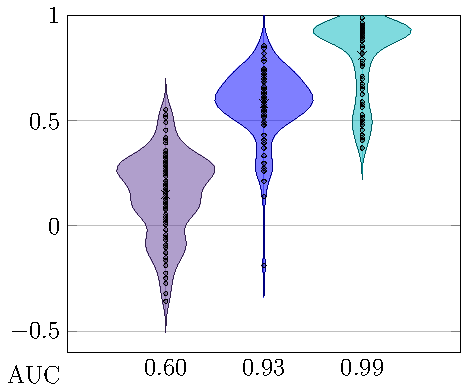
\includegraphics[width=.28\textwidth]{Figures/sec4_4_mlp_auc_shap-figure1.pdf}}%
                \label{subfig:mlp_auc_shap_spearmans}%
            }\hspace{1cm}
            \subfloat[SHAP Relevance]{%
                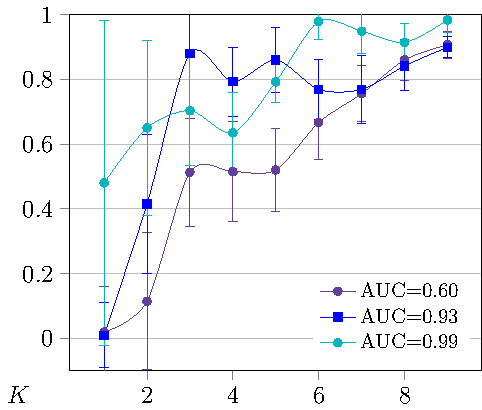
\includegraphics[width=.28\textwidth]{Figures/sec4_4_mlp_auc_shap-figure2.pdf}%
                \label{subfig:mlp_auc_shap_recalls}%
            }\\
            \subfloat[LIME Directionality]{%
                \raisebox{.2cm}{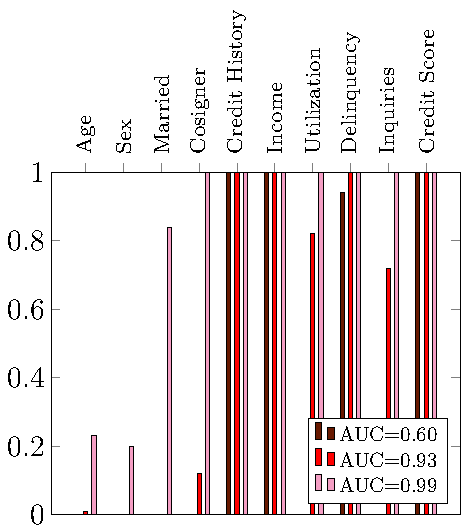
\includegraphics[width=.28\textwidth]{Figures/sec4_4_mlp_auc_lime-figure0.pdf}}%
                \label{subfig:mlp_auc_lime_sign_accs}%
            }\hspace{1cm}%\hfill
            \subfloat[LIME Concordance]{%
                \raisebox{.05cm}{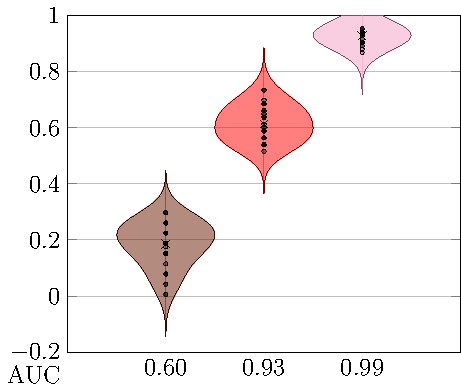
\includegraphics[width=.28\textwidth]{Figures/sec4_4_mlp_auc_lime-figure1.pdf}}%
                \label{subfig:mlp_auc_lime_spearmans}%
            }\hspace{1cm}
            \subfloat[LIME Relevance]{%
                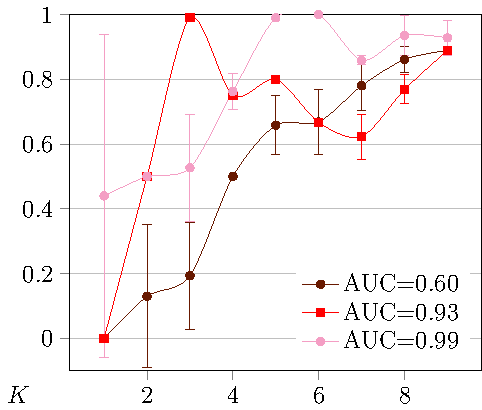
\includegraphics[width=.28\textwidth]{Figures/sec4_4_mlp_auc_lime-figure2.pdf}%
                \label{subfig:mlp_auc_lime_recalls}%
            }\\
            \caption{Comparisons of results for our three metrics for SHAP and LIME when explaining $\mathcal{M}_1$ with AUC=.6, $\mathcal{M}_2$ with AUC=0.92, and $\mathcal{M}_3$ with AUC=.99}
            \label{fig:mlp_auc_increase}
        \end{figure}

    
    %https://stats.stackexchange.com/questions/15011/generate-a-random-variable-with-a-defined-correlation-to-an-existing-variables
    \subsubsection{Role of Feature Independence}
        \label{sec:role_of_correlation}
        The primary goal of training routines for predictive machine learning algorithms is to construct a mapping from the inputs of a dataset to the outputs that correctly labels unseen data. However, a side effect of this focus on predictive performance is that ML models tend to overvalue features that provide information about multiple other features, as these are strong predictors of the target \citep{scholkopf2021toward}. Therefore, the dependence of features can skew their perceived importance in a model, and this importance may be estimated by an explainer and subsequently used to draw incorrect conclusions about the data.

        In real-world scenarios, features are typically not mutually independent. Thus, while the ideal model might rely predominantly on some features to determine the correct label, $\mathcal{M}$ might rely more on other features. Consequently, $\mathcal{M}$ can arrive at the same predictions through an alternate mapping.  Post hoc explainers then interpret the importance of such features in various ways, further muddying the understanding of features within an ML model.
     %        Underlying all natural phenomena is a tangled web of mechanisms which move together to produce what we can perceive and measure. Consider, for example, the following ground truth model depending on features $X_1$ and $X_2$. Let $\mathcal{G}(X_1,X_2) = \alpha_1 X_1 + \alpha_2 X_2$. In this case, $\alpha_1$ and $\alpha_2$ represent the unambigious separate effects of $X_1$ and $X_2$ on $Y$. However, adding a dependence relation such as $X_2 = \gamma X_1 + \epsilon$ makes importance of $X_1$ and $X_2$ on $Y$ unclear; it is only a matter of opinion and context whether $X_2$ is important at all.

         To demonstrate how interdependent features can impact data-alignment, we generate a modified version of the dataset from Section \ref{sec:data_generation} with mutually independent features. Specifically, in this revised dataset, ``Credit Score" is independent of all other features rather than being derived from ``Credit Utilization," ``Credit Inquiries," ``Delinquencies," and ``Credit History." Additionally, ``Cosigner"  is now modeled as a Bernoulli-distributed random variable which is independent of ``Married." In this case, the marginal effects $\boldsymbol{\beta}$ of $\mathcal{G}$ match the coefficients from Equation (\ref{eqn:gt}). %We normalize the SHAP values in an effort to show how feature independence can affect explanations obtained from SHAP, in spite of its inherent data-misalignment.
        

        We clarify the role of feature independence by comparing the alignment of explanations of models trained on the revised dataset with mutually independent features and the original dataset with interdependent features. We will begin analyzing our results by considering overall data-alignment. Then we examine alignment with respect to ``Married" in order to give an example of how alignment with respect to a feature can be worse if that feature is made to be highly correlated with other features.
        
        Our experiments showed that by making ``Credit Score" and ``Cosigner" independent, data-alignment increased overall and with respect to ``Credit Score" and ``Cosigner" in particular. Figures \ref{fig:shap_corr_accs} and \ref{fig:lime_corr_accs} show that directioinality improved for both SHAP and LIME's with respect to several features, including ``Married" and ``Cosigner." The most notable results come from the significant increases in relevance and concordance, especially for LIME.
        \begin{figure}[ht]
            \subfloat[SHAP Directionality]{%
                \raisebox{.2cm}{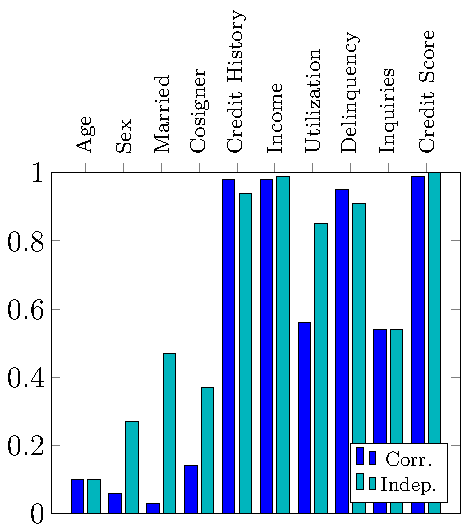
\includegraphics[width=.28\textwidth]{Figures/sec4_3_corr_shap-figure0.pdf}}%
                \label{fig:shap_corr_accs}%
            }\hspace{1cm}%\hfill
            \subfloat[SHAP Concordance]{%
                \raisebox{.05cm}{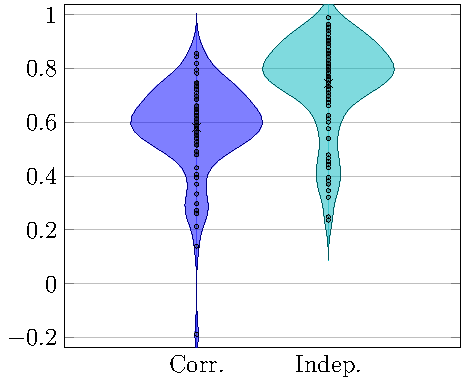
\includegraphics[width=.28\textwidth]{Figures/sec4_3_corr_shap-figure1.pdf}}%
                \label{fig:shap_corr_spearmans}%
            }\hspace{1cm}%\hfill
            \subfloat[SHAP Relevance]{%
                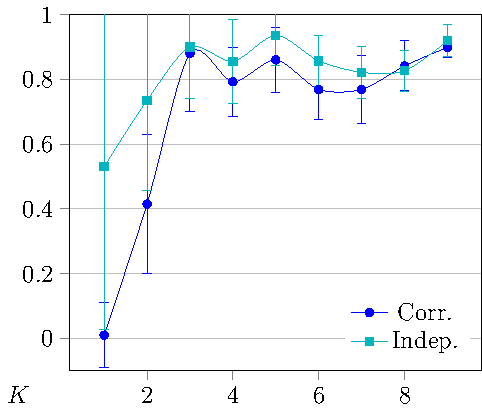
\includegraphics[width=.28\textwidth]{Figures/sec4_3_corr_shap-figure2.pdf}%
                \label{fig:shap_corr_recalls}%
            }\\
            \subfloat[LIME Directionality]{%
                \raisebox{.2cm}{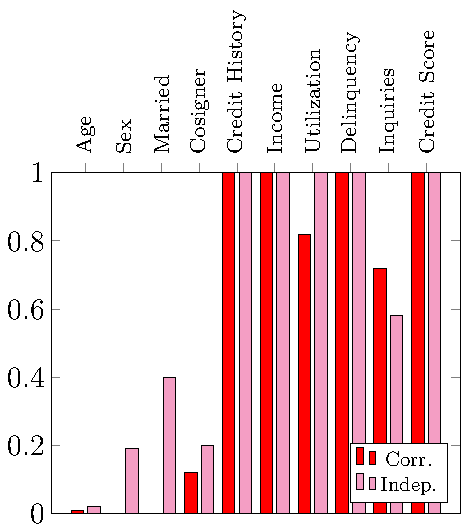
\includegraphics[width=.28\textwidth]{Figures/sec4_3_corr_lime-figure0.pdf}}%
                \label{fig:lime_corr_accs}%
            }\hspace{1cm}%\hfill
            \subfloat[LIME Concordance]{%
                \raisebox{0cm}{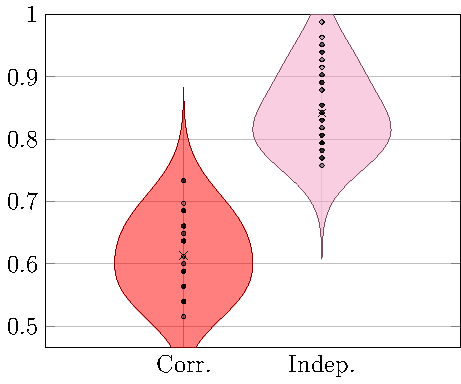
\includegraphics[width=.28\textwidth]{Figures/sec4_3_corr_lime-figure1.pdf}}%
                \label{fig:lime_corr_spearmans}%
            }\hspace{1cm}%\hfill
            \subfloat[LIME Relevance]{%
                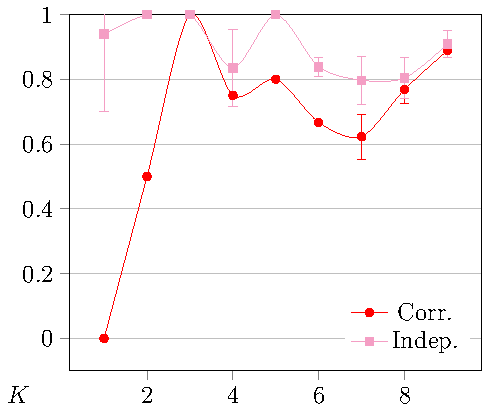
\includegraphics[width=.28\textwidth]{Figures/sec4_3_corr_lime-figure2.pdf}%
                \label{fig:lime_corr_recalls}%
            }\\
            \caption{Comparison of faithfulness of explanations of models trained on data with independent features versus data with two strongly correlated features.}
            \label{fig:lime_shap_colinear}
        \end{figure}
 SHAP saw significant gains in relevance for all $k$ except $k=3,8,9$ (see  Figure \ref{fig:shap_corr_recalls}) as well as a large leap in concordance. Figure \ref{fig:lime_corr_recalls} shows that LIME was adept at identifying the top $k=1,2,3$ most important features when the features were independent while it could rarely (or never) do so when the features were not independent. Its mean concordance was also larger by about $.2$. It is evident from our results that the interdependence of features obfuscates explainers and leads to incorrect feature importance.    

    %\paragraph{Lower Alignment For Correlated Features In Particular}
            %We showed that, when explaining predictions of models with similar predictive performance trained on two similar datasets that differ by virtue of their features being mutually independent (or not), the explanations of the model trained on the data with mutually independent features were more data aligned. One of the differences between the two datasets was that in the original, being married increased the chance that an applicant had a cosigner, while in the variant they were independent. In this experiment, we will show how an example of how marital status influencing cosigner posession, a more important feature for loan approval, is associated with lower data-alignment of explanations with respect to marital status in particular.
        
            Figure \ref{fig:marital_sign_accs} shows bar plots of the directionality achieved by SHAP and LIME with respect to ``Married" before and after making ``Cosigner" depend on ``Married." The bar plots show that the addition of dependencies between features is associated with a loss of the ability to give ``Married" the correct sign for both SHAP and LIME. Figure \ref{fig:marital_rank_diff} shows the distributions of the absolute differences between the given and correct rank for ``Married" before and after introduction of correlation. We see that for both SHAP and LIME, the average ranking error for ``Married" is much smaller when the features are mutually independent than otherwise. These results suggest that it may be more difficult for explainers to extract correct information about the individual marginal effects of interdependent features.
            \begin{figure}[ht!]
                \centering
                \begin{subfigure}{.28\textwidth}
                  \centering
                  \captionsetup{justification=centering}
                  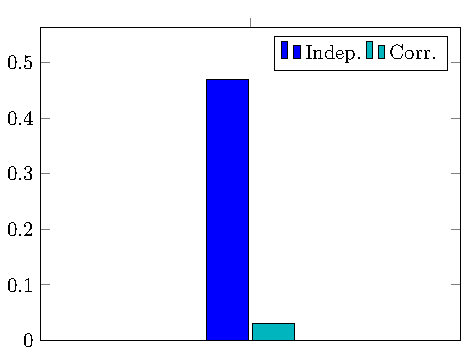
\includegraphics[width=\textwidth]{AppendixFigures/apx_marital-figure1.pdf}%{Figures/fig_age_col.pdf}%{Figures/lime_spearman_colinear.png}
                                %\includegraphics[width=.9\linewidth]{Figures/lime_shap_Spearman_magnitude.png}
    
                  \caption{SHAP}%Spearman rank correlations of ranked feature importance magnitudes from LIME against the true ranked magnitudes from $\mathcal{G}$.}
                   \label{fig:marital_sign_accs_shap}
                \end{subfigure}%
                \hspace{3cm}
                \begin{subfigure}{.28\textwidth}
                  \centering
                     \captionsetup{justification=centering}
                  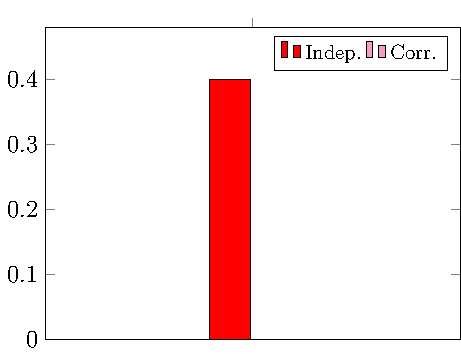
\includegraphics[width=\textwidth]{AppendixFigures/apx_marital-figure0.pdf}%{Figures/fig_score_col.pdf}%{Figures/shap_spearman_colinear.png}
    
                  %\includegraphics[width=.9\linewidth]{Final_Figures/fig9b.png}%{Figures/shap_spearman_colinear.png}
                  \caption{LIME}%Spearman rank correlations of signed feature importance magnitudes from SHAP and LIME against the true ranking from $\mathcal{G}$.}
                   \label{fig:marital_sign_accs_lime}
                \end{subfigure}
                
                \caption{Bar charts showing how SHAP and LIME (almost) never can correctly identify the sign of ``Married" when it is used to determine ``Cosigner."}%rankings of age and credit score change from when being independent to when credit score becomes a function of age}
                \label{fig:marital_sign_accs}
            \end{figure}

            \begin{figure}[ht!]
                \centering
                \begin{subfigure}{.28\textwidth}
                  \centering
                  \captionsetup{justification=centering}
                  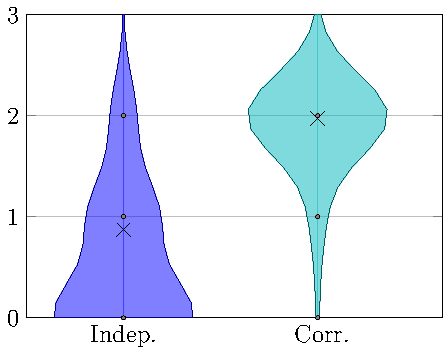
\includegraphics[width=\textwidth]{AppendixFigures/apx_marital-figure2.pdf}%{Figures/fig_age_col.pdf}%{Figures/lime_spearman_colinear.png}
                                %\includegraphics[width=.9\linewidth]{Figures/lime_shap_Spearman_magnitude.png}
    
                  \caption{SHAP}%Spearman rank correlations of ranked feature importance magnitudes from LIME against the true ranked magnitudes from $\mathcal{G}$.}
                   \label{fig:marital_rank_diff_shap}
                \end{subfigure}%
                \hspace{3cm}
                \begin{subfigure}{.28\textwidth}
                  \centering
                     \captionsetup{justification=centering}
                  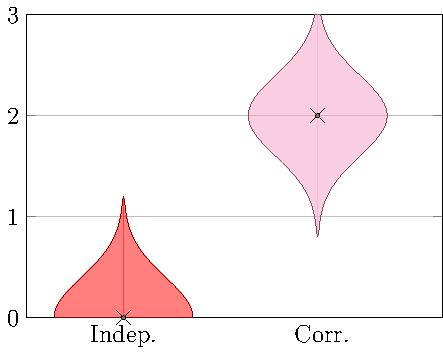
\includegraphics[width=\textwidth]{AppendixFigures/apx_marital-figure3.pdf}%{Figures/fig_score_col.pdf}%{Figures/shap_spearman_colinear.png}
    
                  %\includegraphics[width=.9\linewidth]{Final_Figures/fig9b.png}%{Figures/shap_spearman_colinear.png}
                  \caption{LIME}%Spearman rank correlations of signed feature importance magnitudes from SHAP and LIME against the true ranking from $\mathcal{G}$.}
                   \label{fig:marital_rank_diff_lime}
                \end{subfigure}
                
                \caption{Violin plots showing the differences between the given rank and true rank of ``Married" depending on whether ``Married" influences ``Cosigner." Lower is better.}%rankings of age and credit score change from when being independent to when credit score becomes a function of age}
                \label{fig:marital_rank_diff}
            \end{figure}
    
    \subsection{Discussion}
            Since researchers cannot directly access the ground truth model $\mathcal{G}$ and can only interact with an intermediary machine learning model $\mathcal{M}$, the process of explanation is bifurcated into two distinct stages: the prediction stage and the explanation stage. To generate explanations that accurately reflect the marginal effects, one must navigate challenges that may arise in either stage, necessitating additional assumptions about the data, $\mathcal{M}$, and the explanation tool $\mathcal{E}$. Crucially, $\mathcal{E}$ must possess the ability to accurately capture information regarding the marginal effects. The discussion in Section \ref{sec:theoretical_considerations} describes theoretically why SHAP and LIME are inherently incapable of extracting even qualitative information (e.g. the sign) about the true marginal effects in practice. In addition, even if we presume $\mathcal{E}$'s competence in recovering the actual marginal effects, it is essential for $\mathcal{M}$ to closely approximate $\mathcal{G}$, ensuring that information about the marginal effects is indeed present within $\mathcal{M}$. Insights from Section \ref{sec:causes_of_misalignment} indicate that $\mathcal{M}$'s ability to achieve high predictive accuracy, especially when trained on data featuring mutually independent variables, significantly facilitates the extraction of the marginal effects. However, \textbf{SHAP and LIME being data-misaligned appears to be a general phenomenon}, which is more severe when \textit{a model has low predictive performance, the features are not mutually independent, or there are a large number of features}. 


% \section{Inconsistency of Post Hoc Explanations}
%     \label{sec:inconsistency}
%     Another major issue post hoc explanations  suffer from is inconsistency, which refers to one or more post hoc explainers providing conflicting information about the marginal effects. Inconsistency is a source of confusion and frustration because without sufficient domain knowledge, misaligned explanations cannot be distinguished from aligned ones. Inconsistency can facilitate generation of invalid hypotheses and invalid inference because users without domain knowledge that are not able to account for inconsistency may be forced to make arbitrary selections of explanations. 

%     Explanation inconsistency has to do with the \textit{model being explained} (i.e., $\mathcal{M}$) and the \textit{explainers} (i.e., $\mathcal{E})$. Fixing one explainer and varying $\mathcal{M}$  may yield differing hypotheses about the marginal effects. This variation is due to the different ways in which models capture and approximate the ground truth ($\mathcal{G}$) and their unique decision-making processes, which can significantly diverge even when their predictions appear similar. Factors such as the dataset characteristics and the internal mechanisms and structures of $\mathcal{M}$ influence these outcomes. Conversely, for a fixed $\mathcal{M}$, explanations could still vary due to inherent differences among the explainers or differing configurations of an explainer's hyperparameters. We provide in Appendix Section \ref{apx_sec:appendix_inconsistency} a set of experiments that demonstrate how inconsistency arises with different combinations of explanation methods and models. For example, we show that both the feature rankings and signs from pairs of SHAP and LIME explanations of the same prediction are usually different.

%     In Appendix Section \ref{apx_sec:instability} we also explore a more general form of inconsistency known as instability. Inconsistency of explanations for similar inputs is called instability. Instability can manifest when, e.g., two applicants with similar profiles get different explanations and can lead to uncertainty about which explanation better represents the marginal effects and possibly unfounded suspicions that the decision process is unfair. 


          
%           %At any rate, the issue of inconsistency makes it difficult to justify any one explanation or pipeline configuration if one does not have sufficient domain knowledge, since alternatives abound with equal plausibility. It follows that researchers who wish to use SHAP or LIME to generate hypotheses about their data should take care in doing so. Researchers should be reticent if considering proclaiming that they have identified some novel phenomena via post hoc feature importance values since such novelty could merely be an artifact of inconsistency. Inconsistency thus facilitates generation of invalid hypotheses and invalid inference because users without domain knowledge that are not able to account for inconsistency are forced to make arbitrary selections of explanations. %We also discussed how the volatility of the decision boundary of $\mathcal{M}$ in comparison to the volatility of the decision boundary of $\mathcal{G}$ affects explanation stability. Explaining an underfit $\mathcal{M}$ as part of a fairness audit of $\mathcal{G}$ could cause unfairness to go unnoticed. Conversely, explanations of similar inputs to an overfit $\mathcal{M}$ could be dissimilar and cause confusion and make neither explanation justifiable. %Consider, for example, how Figure \ref{fig:lime_rankings_mag} shows that LIME may indicate that the least important feature is the most important (and vice versa).
         



\section{Mitigation Strategies}
    \label{sec:mitigation_strategies}
    In this section, we use the results of our experiments and the implications of the theoretical results from Section \ref{sec:theoretical_considerations} to propose and test some simple mitigation strategies for misalignment. The strategies we propose here are meant to be sufficiently simple to understand and use such that they form a platform for further exploration and experimentation. We soften the impact of our choices for the data and model in this section by using the version of our dataset with mutually independent features and an NN with accuracy and test set ROC AUC equal to $.99$ in each experiment, unless otherwise stated. To begin the section, we will introduce the criteria we use to test if a strategy improves data-alignment over a baseline with respect to directionality, concordance, and relevance. Then we describe and demonstrate our mitigation strategies, starting with those that are specific to SHAP or LIME and concluding with generally applicable strategies. Using our definitions of improvement, the mitigation strategies we propose are all effective with respect to at least one of the metrics. We provide results for less effective mitigation strategies in Appendix Section \ref{apx_sec:additional_mitigations}. 

    %\subsection{Mitigation Strategies for misalignment}
    %\label{sec:incorrectness_mitigation} %\textcolor{red}{move this to the end of section 4. this is the mitigation strategy for incorrectness}
    
        %We propose a few intuitive mitigation strategies for explanation faithfulness based on data pre-processing and, model training, and explainer hyperparameters. We first demonstrate the truth of Corrolaries 1 and 2 from Section \ref{sec:theoretical_considerations}. We then verify that ensuring both that $\mathcal{M}$ has high test set accuracy and that its training data has no unobserved, correlated, or confounded features is associated with increased explanation quality. The next strategy involves ensuring that $\mathcal{M}$ has high test set ROC AUC. The final strategy involves ensuring that the underlying model of $\mathcal{E}$ correctly classifies the input being explained. When demonstrating the first, third, and fourth strategies, the training data do not have unobserved, correlated, or confounded features in order to isolate the roles of $\mathcal{E}$ and $\mathcal{M}$. 
    \subsection{Testing Improvement}
        \label{sec:improvement}
        This section introduces the hypothesis testing framework that we use to characterize whether an explanation method $\mE^\prime$ improves over a baseline explanation $\mE$ in terms of directionality, concordance, and relevance. All details, including statements of the null and alternative hypotheses we use, can be found in Appendix Section \ref{apx_sec:hypothesis_testing}.
        
        
        The underlying idea of our identification of improvement is to test if the mean(s) of metrics of interest is(are) higher for $\mE^\prime$ than for $\mE$ using Wilcoxon signed-rank tests on the location of mean of differences from  matched samples.
        %When testing for improvement of consistency of feature importance signs, we use one-sided McNemar tests for whether pairs of the pipeline with the mitigation strategy applied and baseline disagree on feature importance signs at the same rate. 
        All of our tests are performed with a significance level of $\alpha=.05$. 
        
        Our tests of improvement differ between concordance and directionality/relevance because the latter are feature-wise metrics. Since the computation of concordance involves all features, testing if it has been improved consists of a single Wilcoxon signed-rank test involving the matched pairs of concordances for each test instance. However, since directionality is computed for each feature and relevance is computed for $k=1,\ldots,D-1$, we formulate a rather strict characterization of improvement of $\mE^\prime$ over $\mE$ that takes into account the possibility that, e.g., $\mE^\prime$ may have higher relevance than $\mE$ for $k=1,2,3$ but lower relevance for $k=4$. Our tests for directionality and relevance are meant to capture when $\mE^\prime$ has a statistically significant improvement over $\mE$ in at least one respect and is not significantly worse than $\mE$ in any respect. What this means for directionality is that directionality must have a statistically significant increase for at least one feature and no statistically significant decrease for any feature. Similarly, for relevance, it means that the mean relevance of $\mE^\prime$ must be significantly larger than that of $\mE$ for at least one $k$, and not significantly smaller for any $k$.   
        
        
     


    \subsection{Explainer Specific Strategies}
        Before discussing general-use strategies, we will present three strategies applicable only to SHAP or LIME (but not both). 

            \subsubsection{Normalizing The Shapley Value}
                As discussed in Section \ref{sec:theoretical_considerations}, it follows directly from the theory underlying SHAP that SHAP explanations do not naturally extract the marginal effect values $\boldsymbol{\beta}$. It is therefore worthwhile to seek practical ways to modify our usage of SHAP. Since Equation (\ref{eqn:shap_gt}) showed that SHAP returns $e_{\text{SHAP}}(\mathbf{x}^{(i)})=\boldsymbol{\beta}^T(\mathbf{x}^{(i)} - \bar{\mathbf{x}})$ instead of $\boldsymbol{\beta}$, we proposed in Section \ref{sec:theoretical_considerations} to instead take the importance of feature $j$ to be $e_{\text{SHAP}}(x^{(i)}_j) / (x^{(i)}_j - \bar{x}_j)$ where $\bar{x}_j$ is the empirical mean of feature $j$ from the training data because this expression should be approximately $\beta_j$. Our experiments confirmed the advantage of this strategy: Figure \ref{fig:shap_dividex_corr} showed that unmodified SHAP explanations perform about as well as random explanations with respect to our three metrics while the normalized SHAP explanations performed significantly better in all three metrics. Therefore, all of our mitigation strategies involving SHAP will make use of the normalization scheme by default.

                %In addition, the normalized SHAP explanations were more consistent across individuals (recall that Figure \ref{fig:shap_dividex_spearmans} showed that the concordance distribution for normalized SHAP explanations had a significantly smaller region of support which, importantly, was centered at a larger value than the mean concordance of the unmodified SHAP explanations). 
                %%Since these results were produced using the version of our dataset with correlated features, we additionally provide a comparison of SHAP without and with normalization when the input features are independent in Appendix Section \ref{apx_sec:shap_norm_indep}.



        
        \subsubsection{Increasing $\nu$ and $N$ for LIME } 
            \label{sec:lime_params}
            Our theoretical results on LIME from Section \ref{sec:theoretical_considerations} imply that LIME's kernel bandwidth $\nu$ and number of perturbed samples $N$ need to be large in order for $e_{\text{LIME}}(x_j)$ to be close to $\boldsymbol{\beta}$, so this section will experiment with how their respective sizes affect explanation quality. To show the impact of $\nu$ and $N$, we compare the data-alignment of explanations from LIME explanations using the default choices of $\nu = .75\sqrt{D}$ (where $D$ is the number of features) and $N=1000$ used in the official LIME implementation \citep{ribeiro16lime} with explanations LIME explanations which use the larger values $\nu=N=10000$. 
            
            Figure \ref{fig:lime_tuning} shows that increasing the number of samples $N$ and the kernel bandwith $\nu$ improved data-alignment. For example, for directionality, increasing $\nu$ and $N$ improved directionality  significantly  ``Age," ``Cosigner," and ``Sex." The larger $\nu$ and $N$ also resulted in pairs of rankings whose concordances were significantly larger on average.%; our test for equally consistent rankings had $p<.001$. %The plot of $\text{relevance}_k$ shows that using $\nu=n=10000$ netted a strict advantage for correctly ranking the features which were not the most or least important. That is, for $k=1$ the results were identical and for $k=2,8$ we fail to reject the null hypothesis of equal relevances with a p-values of $0.08$ and $0.12$ respectively, but we do reject the null hypotheses for $k=3,\ldots,7$ with p-values of $9.14e-5$, $4.56e-4$, $1.71e-7$, $2.64e-11$, and $5.90e-12$.
        
            \begin{figure}[ht!]
                \centering
                \begin{subfigure}[t]{.28\textwidth}
                  \centering
                  \captionsetup{justification=centering}
                      \raisebox{.2cm}{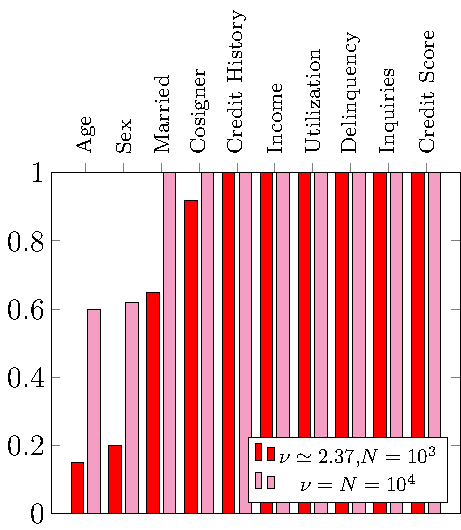
\includegraphics[width=\textwidth]{Figures/sec4_4_lime-figure0.pdf}}%{Figures/lime_shap_Spearman_magnitude.png}
    
                  \caption{Directionality}%Spearman rank correlations of feature importance magnitudes from SHAP and LIME against the true ranking from $\mathcal{G}$. }
                   \label{fig:lime_tuning_sign_accs}
                \end{subfigure}%
                \hspace{1cm}
                \begin{subfigure}[t]{.28\textwidth}
                  \centering
                   \captionsetup{justification=centering}
                  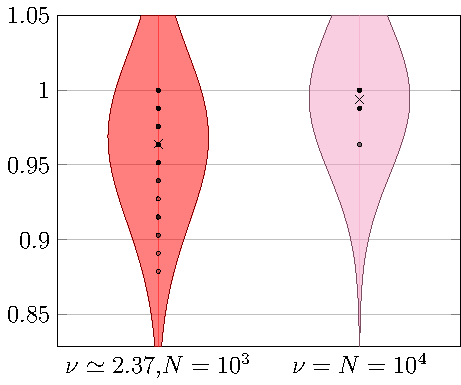
\includegraphics[width=\textwidth]{Figures/sec4_4_lime-figure1.pdf}%{Figures/lime_shap_Spearman_signed.png}
                  \caption{Concordance}%Spearman rank correlations of signed feature importance from SHAP and LIME against the true ranking from $\mathcal{G}$.}
                   \label{fig:lime_tuning_spearmans}
                \end{subfigure}
                \hspace{1cm}
                \begin{subfigure}[t]{.28\textwidth}
                  \centering
                   \captionsetup{justification=centering}
                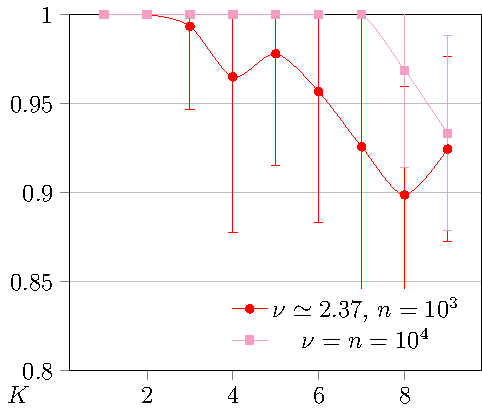
\includegraphics[width=\textwidth]{Figures/sec4_4_lime-figure2.pdf}%
                \caption{Relevance}%The average and standard error of recall of SHAP and LIME when attempting to capture the top K most important features to $\mathcal{G}$ when explaining $\mathcal{M}$, for varied $K=1,2,3,...$ number of features.}
                \label{fig:lime_tuning_recalls}
                \end{subfigure}
                \caption{Comparison of LIME explainer with default settings $\nu=.75\sqrt{D}\simeq 2.37,\ N=1000$ versus $\nu=N=10000$ with respect to our three metrics}
               \label{fig:lime_tuning}
            \end{figure} 
% \tw{Figure 8c looks so weird. How come it's a decreasing curve?}
            \subsubsection{Averaging Explanations of One Model by Different Explainers}
            \label{sec:averaging_one_explainer}
            Since there exists randomness in LIME (the random seed, the sampling, etc.), the feature importance may not be exactly the same if LIME is run multiple times. This is a problematic property of LIME since its explanations could be inconsistent \citep{alvarez18robustness} as a result of this randomness. 
        However, we propose that it can actually be leveraged into an advantage. Each explanation likely has at least a modicum of truth, and so an aggregation strategy for explanations may increase the signal-to-noise ratio. We propose here one simple realization of this general idea. Given one ML model $\mathcal{M}$ and instance $\mathbf{x}$, we leverage the abundance of possible LIME explanations of $\mathcal{M}(\mathbf{x})$ by averaging the feature importance values given by a set of LIME explainers with different random seeds.
        
            To test this technique, we compare explanations averaged from 100 LIMEs with explanations from one LIME of $M=100$ applications. %The averaged explanation for each applicant is constructed by averaging over the feature importance values from 100 LIME explanations of the applicant, where the 100 explainers are created using random seeds $1,\ldots,100$ and default settings. .  %We repeat this with $\nu=n=10000$. 
            Our statistical tests of improvement concluded that directionality, concordance, and relevance were significantly improved by using averaged instead of single LIME explanations. Averaging LIME explanations resulted in an enhanced ability to find the sign of ``Age," ``Sex," ``Married" and ``Cosigner" (see Figure \ref{fig:lime_avg_sign_accs}). %The mitigation did not change the assignment of the other features but we were able to reject the null hypothesis of equal sign accuracies for ``Age," ``Cosigner," ``Married," and ``Sex" all with with $p<.001$. %$3.32e-3$, $2.34e-3$, $3.17e-5$, and $2.12e-6$, respectively.
            Moreover, the concordances of the averaged explanations were significantly higher than those of the single explanations. Thus, when an explanation method has hyperparameters that affect the explanations it produces, it may be worthwhile to leverage the explanations of multiple instances of that explainer.%; we rejected the null hypothesis of equal concordances with $p<.001$.%a p-value of $7.39e-12$. %Figure \ref{fig:lime_avg_recalls} also shows that the averaged explanations were more likely to identify the features which were not the most or least important. 

            % \begin{table}[]
            % \centering
            % \begin{tabular}{|l|l|l|l|l|l|l|l|l|l|}
            % \hline
            % Age  & Cosigner & Credit History & Credit Score & Delinquency & Income & Inquiries & Married & Sex & Utilization \\ \hline
            % 0.98 & 1.20e-7   & n/a            & n/a          & n/a         & n/a    & 0.50      & 1.11e-4 & .12 & n/a         \\ \hline
            % \end{tabular}
            % \caption{p-values for improvement to consistency of feature importance signs by using averaged LIME explanations. Values are listed as ``n/a" if both pairs of explanations always found the correct sign for the corresponding feature.}
            % % \label{tab:lime_avg_sign_con}
            % \end{table}
                             
            \begin{figure}[!h]
            \centering
                \begin{subfigure}[t]{0.28\textwidth}
                \centering
                \raisebox{.2cm}{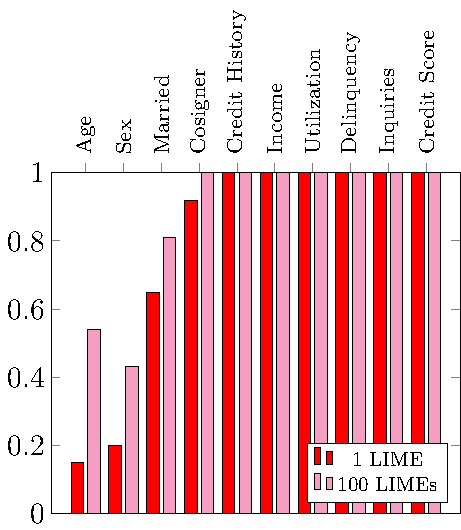
\includegraphics[width=\textwidth]{Figures/sec5_2_lime_avg-figure0.pdf}}
                \caption{Directionality} \label{fig:lime_avg_sign_accs}
            \end{subfigure}\hspace{1cm}
            \begin{subfigure}[t]{0.28\textwidth}
                \centering
                \raisebox{.05cm}{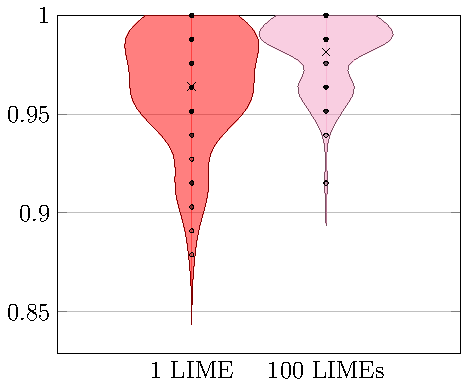
\includegraphics[width=\textwidth]{Figures/sec5_2_lime_avg-figure1.pdf}}
                \caption{Concordance} \label{fig:lime_avg_spearmans}
            \end{subfigure}\hspace{1cm}
             \begin{subfigure}[t]{0.28\textwidth}
                \centering
                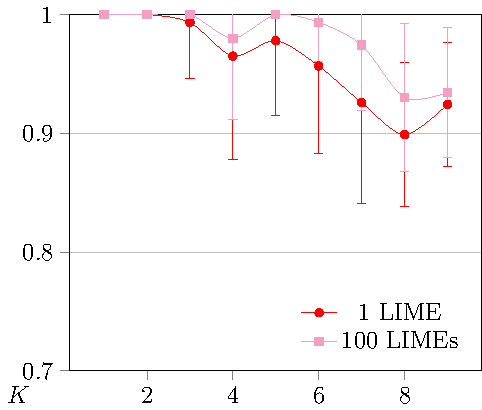
\includegraphics[width=\textwidth]{Figures/sec5_2_lime_avg-figure2.pdf}
                \caption{Relevance}
                \label{fig:lime_avg_recalls}
            \end{subfigure}
            \caption{Comparisons of results for our three metrics for  explanations of an NN $\mathcal{M}$ by 1 LIME explainer versus those created by averaging the feature importance values of 100 LIME explanations of $\mathcal{M}$}\label{fig:lime_avg}
            \end{figure}

                
            %It was also the case that the averaging routine significantly improved consistency. To obtain this result, we created another set of average explanations from 100 more LIME explainers using random seeds $101,\ldots,200$, and tested whether the signs and rankings were more consistent between the two sets of averaged explanations compared to the signs and rankings of the two individual LIME explainers. We rejected the null hypotheses of our tests for equal consistency of feature importance signs in favor of improvement for ``age", ``cosigner", and ``married" all with $p<.001$.%of  $8.65e-3$, $1.20e-7$ and $1.11e-4$, respectively.
            %There was no change for ``credit  history", ``credit score", ``delinquency", ``income", and ``utilization" because both methods were perfect in each case.  With a p-value of $7.60e-15$, we rejected the null hypothesis of our Wilcoxon test that the means of the two concordance distributions are equal in favor of the alternative hypothesis that the mean of the concordance distribution from the averaged explanations is larger. That this is the case is also visually evident from Figure \ref{fig:lime1_v_100_incon}; the concordance distribution of the averaged explanations was more concentrated near 1 and its tail was also shorter. 

            % \begin{figure}[ht!]
            %     \centering
            %     %\begin{subfigure}{.3\textwidth}
            %       \centering
            %       \captionsetup{justification=centering}
            %       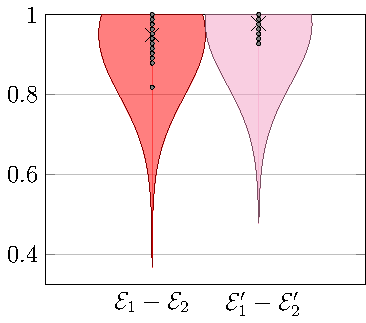
\includegraphics[width=.28\textwidth]{Figs/sec5_2_lime_avg2-figure3.pdf}
            %       \caption{Comparison of concordances between explanations from pairs of individual LIME explainers and between pairs of averaged explanations from two sets of 100 LIME explainers.}%Spearman rank correlations of ranked feature importance magnitudes from LIME against the true ranked magnitudes from $\mathcal{G}$.}
            %        %\label{fig:lime_income}
            %     %\end{subfigure}%
            %     %\caption{}%Violin plots of feature importance values for \emph{income} from SHAP and LIME for cases when \emph{income} is unconfounded and confounded by the unobserved social support feature}
            %     \label{fig:lime1_v_100_incon}
            % \end{figure}
                
    \subsection{General Strategies}
        We now provide three general strategies that can be applied to both SHAP and LIME to produce explanations that are more data-aligned. Note that we have been and will continue using normalized Shapley values, since default SHAP explanations are not better than random with respect to data-alignment. %To show the utility of these strategies for SHAP, we will use normalized SHAP values in each the experiments below. 

        \subsubsection{Optimizing the Tradeoff between Complexity and Predictive Power}
            \label{sec:decreasing_complexity}
            The hypothesis space, which encompasses the set of all possible machine learning models that can be constructed for any dataset of practical utility, is unimaginably large, making model selection challenging from the outset. Further complicating this process is the existence of many models with similar predictive performance, a concept known as the Rashomon set theory \citep{semenova22rashomon}. Given that notions of complexity, such as parameter count, are fundamental distinguishing properties of models, the statistics literature on parsimony in curve fitting often appeals to Occam's razor—plurality should not be posited without necessity—suggesting that simpler models are more likely to be correct than complex ones \citep{popper2005logic}.

            
            For this reason, we designed a mitigation strategy that takes into account the complexity of $\mathcal{M}$. As we established in Section \ref{sec:role_of_predictive_power}, there is an association between the predictive performance of $\mathcal{M}$ and the alignment of post hoc explanations of $\mathcal{M}$ with respect to $\mathcal{G}$. This mitigation strategy proposes ensuring that $\mathcal{M}$ achieves both good predictive performance and minimal complexity.
 %The labels predicted by $\mathcal{M}$ (after thresholding its output probabilities) agreeing with those in the test set is an incomplete representation of faithfulness to $\mathcal{G}$; even if $\mathcal{M}$ had 100\% training and testing accuracy on data with no measurement error, this does not mean $\mathcal{M}=\mathcal{G}$.  Thus, it is worth making an effort not to over-parameterize $\mathcal{M}$. %\tw{The explanation should be moved to earlier this paragraph. WE can use the argument of Ocam's razor, that low complexity is generally preferred. This point should be given a deeper discussion before proposing to get ``minimal complexity"} 
            To implement this strategy, one can iteratively train and evaluate models of successively lower complexity, stopping the process once a reduction in complexity results in a significant decrease in predictive performance.
   \begin{figure}[t!]
            \subfloat[SHAP Directionality]{%
                \raisebox{.2cm}{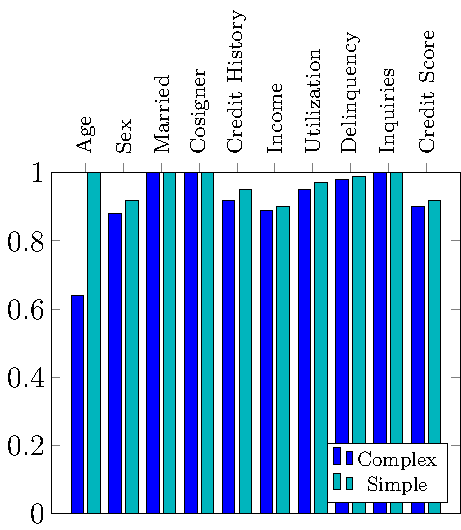
\includegraphics[width=.28\textwidth]{Figures/sec5_mlp_complexity_shap-figure0.pdf}}%
                \label{subfig:decreasing_complexity_shap_sign_accs}%
            }\hspace{1cm}
            \subfloat[SHAP Concordance]{%
                \raisebox{.05cm}{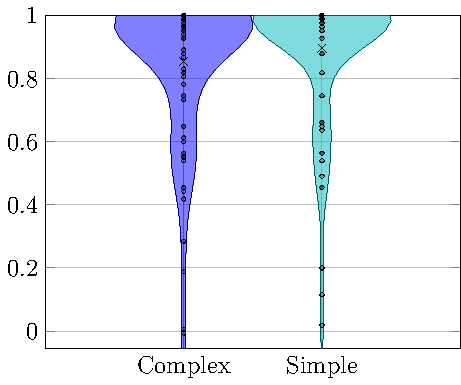
\includegraphics[width=.28\textwidth]{Figures/sec5_mlp_complexity_shap-figure1.pdf}}%
                \label{subfig:decreasing_complexity_shap_spearmans}%
            }\hspace{1cm}
            \subfloat[SHAP Relevance]{%
                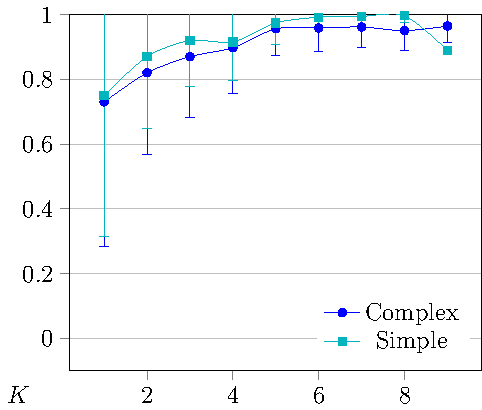
\includegraphics[width=.28\textwidth]{Figures/sec5_mlp_complexity_shap-figure2.pdf}%
                \label{subfig:decreasing_complexity_shap_recalls}%
            }\\
            \subfloat[LIME Directionality]{%
                \raisebox{.2cm}{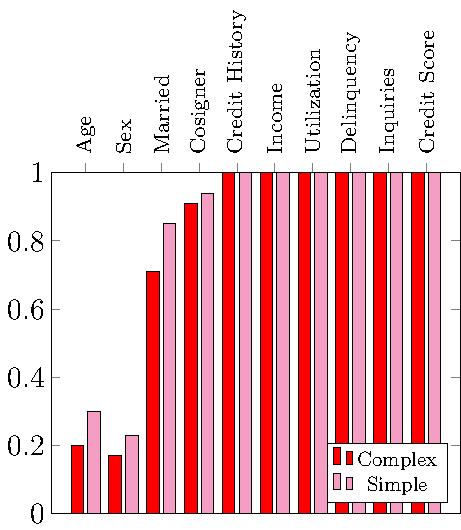
\includegraphics[width=.28\textwidth]{Figures/sec5_mlp_complexity_lime-figure0.pdf}}%
                \label{subfig:decreasing_complexity_lime_sign_accs}%
            }\hspace{1cm}
            \subfloat[LIME Concordance]{%
                \raisebox{.05cm}{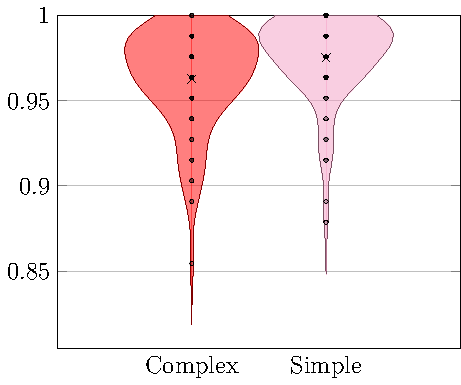
\includegraphics[width=.28\textwidth]{Figures/sec5_mlp_complexity_lime-figure1.pdf}}%
                \label{subfig:decreasing_complexity_lime_spearmans}%
            }\hspace{1cm}
            \subfloat[LIME Relevance]{%
                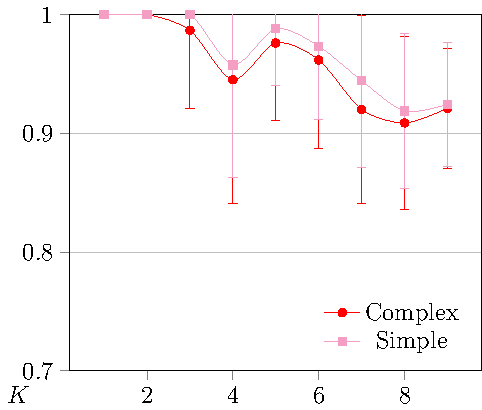
\includegraphics[width=.28\textwidth]{Figures/sec5_mlp_complexity_lime-figure2.pdf}%
                \label{subfig:decreasing_complexity_lime_recalls}%
            }\\
            \caption{Comparisons of results for our three metrics for SHAP (top row) and LIME (bottom row) explanations of equally accurate NNs with high and low complexity.}
            \label{fig:decreasing_complexity}
        \end{figure}
        
            To investigate the trade-off between model complexity and data-alignment, we compare the SHAP and LIME explanations of two neural networks (NNs) with differing complexities but nearly identical predictive performance. The first NN, $\mathcal{M}_1$, has 100 nodes in its hidden layer (the default in sklearn) and achieves a test set AUC of approximately 0.99. The second, simpler NN, $\mathcal{M}_2$, has only two nodes in its hidden layer, yet it still achieves a test set AUC of around 0.98. Figure \ref{fig:decreasing_complexity} visualizes our comparison of the explanations provided by SHAP and LIME for $\mathcal{M}_1$ and $\mathcal{M}_2$. %Additional results and further motivation for this strategy can be found in Appendix Section \ref{apx_sec:appendix_inconsistency}.

            We found that, by explaining the simpler NN $\mathcal{M}_2$ instead of the more complex $\mathcal{M}_1$, it was possible to get more data-aligned explanations. %However, as shown by Figure \ref{fig:decreasing_complexity}, the improvements were marginal for the most part. \textcolor{red}{I don't think so. let's talk about it}. 
            In particular, SHAP's directionality for ``Age and ``Credit History," as well as SHAP's relevance for $k=1,2,4,5,6,7$ were increased significantly. 
           %For SHAP, we reject the null hypothesis of equal sign accuracies only for ``Age" with $p<001$ and ``Credit History" with a p-value of $0.04$. It is evident from Figure \ref{subfig:decreasing_complexity_shap_spearmans} that concordance did not rise significantly; we failed to reject the null hypothesis of equal concordances with a p-value of $.16$. Although relevance worsened for $k=8$ when explaining $\mathcal{M}_2$, the small improvements for $k=1,2,4,5,6,7$ were all statistically significant with $p<.001$ except for $k=4$, which had $p=.05$. 
            For LIME, directionality was improved for ``Married," concordance was significantly improved overall, and relevance was significantly increased for $k=2,6$. Overall, these results suggest that explanations of simpler models can be more data-aligned than explanations of more complex models with equivalent predictive performance. 
            %For LIME, we could only conclude that the directionality of ``Married" improved by rejecting the null hypothesis of equal directionality with a p-value of $0.015$. However, the improvement to concordance was significant, as its test had $p<.001$. As for relevance, the results for $k=1$ were identical and the null hypothesis of equal relevance was rejected in favor of improvement for $k=2,6$ with p-values of $0.02$ and $0.01$. Overall, the results suggest that explanations of simpler models are more data-aligned than explanations of more complex models with equivalent predictive performance. 
            
            A reason that the explanations of the simple model $\mathcal{M}_2$ were more data-aligned is that even though $\mathcal{M}_1$ and $\mathcal{M}_2$ may have similar behavior in how they generate training and test set label predictions, the additional expressive power of $\mathcal{M}_1$ allows the local behavior of its decision boundary to be more erratic. Given that SHAP and LIME are local function approximators, incorrect local behavior of $\mathcal{M}_1$ imposes a limitation on how data-aligned SHAP and LIME can be when explaining $\mathcal{M}_1$. 

            
       

        \subsubsection{Averaging Explanations of Different Models}
           The rapid proliferation of new machine learning models and methods has made it increasingly challenging for researchers to decide which model to use and ultimately explain. Based on the Rashomon set theory \citep{semenova22rashomon,wang2022timbertrek,donnelly2023rashomon}, a straightforward approach to addressing the uncertainty about which black box model to explain is to train multiple models, generate explanations for each, and then average those explanations. This method incorporates diverse information from the hypothesis space under consideration into the final (averaged) explanation.


            With this in mind, we repeat the experiments of Section \ref{sec:evaluating_faithfulness} twice: first using explanations for a single model, and then averaging explanations for 10 unique neural networks (NNs) with ROC AUC scores of at least 0.9. The averaged explanations are constructed separately for SHAP and LIME in the following manner. Given an applicant, 10 explanations are obtained, one for each NN. These explanations are averaged to create a final averaged feature importance vector. We aim to test whether these averaged explanations offer an improvement over singular explanations in terms of data-alignment.
            % PUT THESE DETAILS IN APPENDIX
            %Each NN is trained with 5 hidden layers and for 10 iterations as before, but each NN initializes its training with a different random seed. We control for the inconsistency of the explainers by using default hyperparameters and keeping the random seed of the explainers the same. 
             
            Our feature importance averaging strategy showed some promise but the results of our Wilcoxon tests for improvement of data-alignment were not consistent between SHAP and LIME. The differences are visualized in Figure \ref{fig:mlp_increase}. 
             Regarding SHAP, Figures \ref{subfig:mlp_avg_shap_sign_accs} and Figure \ref{subfig:mlp_avg_shap_spearmans} show that there was a large improvement in directionality for ``Age" and small improvements in directionality for many other features. However, even with the mitigation, SHAP did not have perfect directionality for as many features as LIME did.  It also had no discernible difference in concordance. 
            Showing a stark contrast with SHAP, LIME's directionality, concordance, and relevance were all significantly improved. Directionality for ``Cosigner," ``Married," and ``Sex" were significantly improved. Directionality for the other features was perfect for the other features both with and without the mitigation. In contrast, for SHAP, there was no significant change to directionality for any feature, no significant change to concordance, and no significant change to relevance for any $k$.  Given these results, we can only adduce that this strategy is effective for LIME. In particular, it was effective in increasing directionality and concordance, but not relevance.  %Our results are shown in Figure \ref{fig:mlp_increase}.
            
            %Figure \ref{subfig:mlp_avg_lime_spearmans} shows that LIME's averaged explanations had a slightly larger mean and slightly lower range while Figure \ref{subfig:mlp_avg_lime_spearmans} shows that concordance was almost unchanged for SHAP. Figures \ref{subfig:mlp_avg_lime_sign_accs} and  for LIME and \ref{subfig:mlp_avg_shap_sign_accs} and \ref{subfig:mlp_avg_shap_recalls} show that, with a few exceptions, the averaged explanations were at least as good as the explanations of a single model at identifying feature importance signs and the top-$k$ features. 
            
            %However, the strategy does not seem to be particularly beneficial for finding the top-$k$ features; the curves plotting the recall for SHAP and LIME in Figures \ref{subfig:mlp_avg_lime_recalls} and \ref{subfig:mlp_avg_shap_recalls} are nearly identical for the averaged and single explanation.%Figure \ref{fig:mlp_avg_recalls} also shows that the curves representing the relationships between $K$ and recall for $n=100$ bound the other curves from above. Therefore, this strategy appears to be effective in reducing both misalignment and inconsistency.

            % This strategy can be seen as a simplified version of \citep{donnelly2023rashomon}. Instead of leveraging explanations of good models trained on one dataset, they leverage explanations of optimal decision trees or GAMs trained on bootstraps of one dataset. At the time of writing, their method is not valid for more complex models like neural networks. It also produces statistics for feature importance instead of singular feature importance values. 
    

        \begin{figure}[t!]
            \subfloat[SHAP Directionality]{%
                \raisebox{.2cm}{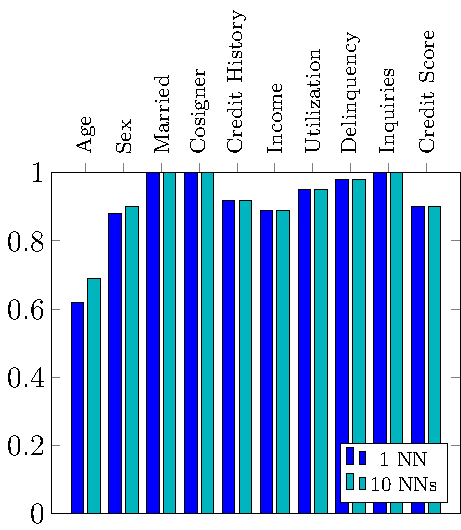
\includegraphics[width=.28\textwidth]{Figures/sec5_2_mlp_avg_shap-figure0.pdf}}%
                \label{subfig:mlp_avg_shap_sign_accs}%
            }\hspace{1cm}
            \subfloat[SHAP Concordance]{%
                \raisebox{.05cm}{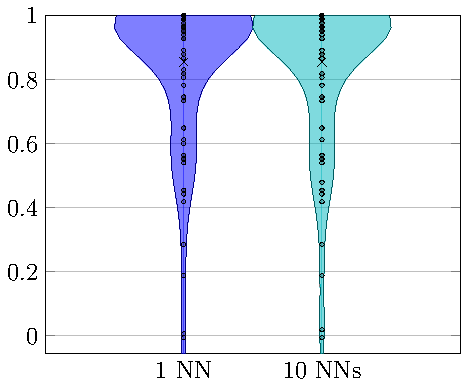
\includegraphics[width=.28\textwidth]{Figures/sec5_2_mlp_avg_shap-figure1.pdf}}%
                \label{subfig:mlp_avg_shap_spearmans}%
            }\hspace{1cm}
            \subfloat[SHAP Relevance]{%
                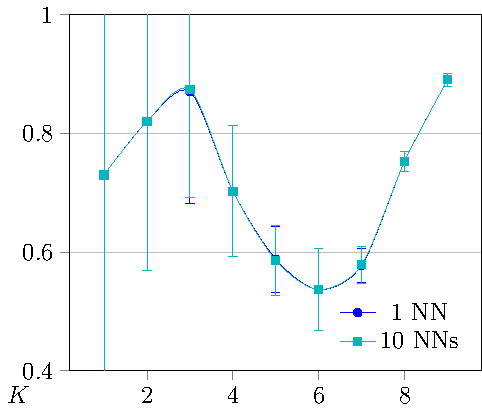
\includegraphics[width=.28\textwidth]{Figures/sec5_2_mlp_avg_shap-figure2.pdf}%
                \label{subfig:mlp_avg_shap_recalls}%
            }\\
            \subfloat[LIME Directionality]{%
                \raisebox{.2cm}{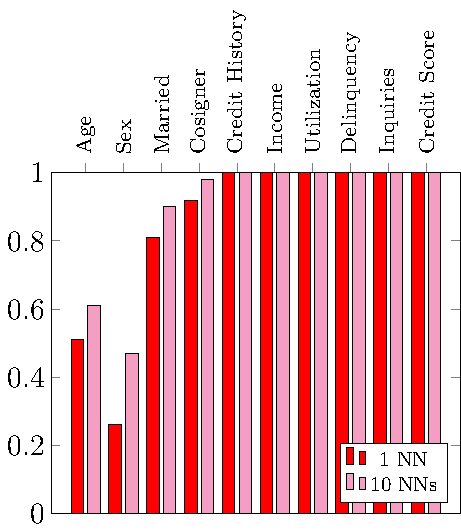
\includegraphics[width=.28\textwidth]{Figures/sec5_2_mlp_avg_lime-figure0.pdf}}%
                \label{subfig:mlp_avg_lime_sign_accs}%
            }\hspace{1cm}
            \subfloat[LIME Concordance]{%
                \raisebox{.05cm}{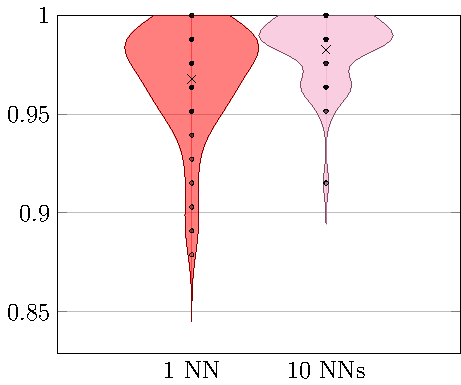
\includegraphics[width=.28\textwidth]{Figures/sec5_2_mlp_avg_lime-figure1.pdf}}%
                \label{subfig:mlp_avg_lime_spearmans}%
            }\hspace{1cm}
            \subfloat[LIME Relevance]{%
                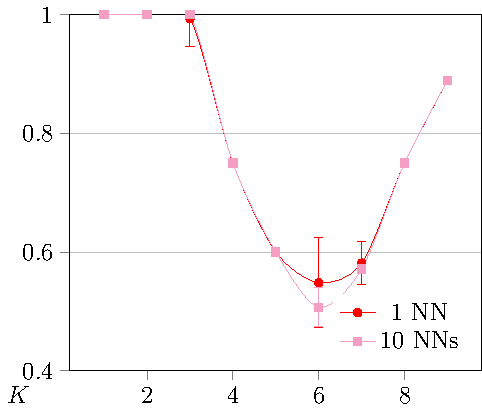
\includegraphics[width=.28\textwidth]{Figures/sec5_2_mlp_avg_lime-figure2.pdf}%
                \label{subfig:mlp_avg_lime_recalls}%
            }\\
            \caption{Comparisons of data-alignment for SHAP (top row) and LIME (bottom row) explanations of 1 NN versus explanations constructed by averaging the feature importance values of 10 NNs.}
            \label{fig:mlp_increase}
        \end{figure}
        

   
    
    \subsection{Summary and Discussion of Mitigation Strategies}
            \label{sec:summary_and_strategies}
            The primary results of our mitigation experiments suggest that when using SHAP, it is advisable to normalize the Shapley values. For LIME, it may be beneficial to aggregate the explanations from multiple LIME instances, with each individual LIME explainer configured with large values for $\nu$ and $N$. Additionally, it is recommended to select black box models that strike an optimal balance between complexity and predictive power, and to average explanations across ensembles of explainers and/or models.
            %It makes less sense to combine explanations of a single model than explanations of multiple models because of the idea that ``all models are wrong." 

            We discuss two unsuccessful mitigation strategies in the Appendix, both based on aggregating explanations of a single black box. The first exchanges the previously used simple averaging of LIME explanations for a method of ranked choice voting known as the Borda count and the second averages SHAP and LIME explanations together. We believe that a core reason why these two strategies were unsuccessful is that they only involve a single black box model. Finding common (valid) patterns within multiple black boxes is possible by aggregating explanations of those models, whereas aggregations of explanations of a single black box can at best reveal the single, imperfect, pattern identified by that black box. Ignoring bias and error in the dataset, each explanation has two layers of approximation error with respect to the ground truth, whereas each black box has only its own approximation error and captures different patterns in the training data. Thus, researchers may find averaging feature importance values obtained by many models both a useful and intuitive strategy \citep{dong2020variable,donnelly2023rashomon}.  %With the configuration of data and model we used, the local error rates of both SHAP and LIME were skewed to the right, implying that the mean local fidelity over samples of SHAP and LIME models can decrease as the sample size increases. However, it is difficult to validate this claim because the local fidelity of SHAP and LIME is not an especially good measure of how faithful their explanations are to $\mathcal{G}$. That averaging SHAP and LIME together did not yield a consistent and substantial advantage is likely due to the simplicity of the technique. For this reason, we suggest that more research be done on this topic. 
            
            Researchers who would like to investigate the importance and impact of features in the data may find exploring the following general strategy useful.
        %First, the choice of explainer(s) used for the strategy should be guided by user preference for the types of feature importance outlined in Section \ref{sec:theoretical_considerations}. For example, LIME should be preferred to SHAP if  $\boldsymbol{\beta}$ is considered to be the ground truth feature importance representation.  %construct average explanations over a collection of good LIME explanations of good models. If situational importance is more suitable than theoretical importance for the application, researchers should instead average over SHAP explanations of good models. 
            When starting the prediction stage, the dataset should be pre-processed to remove highly correlated features.\footnote{If possible, adjustments can be made to account for confounding. Tools like E-values\citep{gaster2023quantifying} and Pearl's backdoor criterion can be used for this purpose.} % The causal graph can be estimated using Bayesian Networks if sufficient domain knowledge is available.}
            Having pre-processed the data, researchers are encouraged to train $B\geq 1$ black box models with simple enough decision boundaries to not lose too much predictive performance compared to more complex models.\footnote{Ideally, Rashomon sets of models would be constructed and the simplest models in them would be collected. However, at the time of writing, this is only possible for decision trees and GAMs.} To construct a more robust explanation of a model's predicted outcome for an instance, the results of multiple explainers of that model can be aggregated by, e.g., averaging the feature importance values for each feature over the explainers. An even more robust final explanation for an instance can be produced by averaging over the importance values given in the $B\times E$ explanations of the predictions of $B$ models by $E$ explainers.
          


\subsection{Case Study Using Real Data and Econometric Method}
    \label{sec:case_study}
    To validate the efficacy of our mitigation strategies and demonstrate their practical application, we test whether they provide an advantage over the default usage of SHAP and LIME in extracting the same marginal effects as those identified in an econometric study on home loan application approvals \citep{bane2006econometric}. Specifically, we will adapt the framework outlined in Section \ref{sec:summary_and_strategies} to create mitigated pipelines for SHAP and LIME separately.
    
   The home loan dataset is publicly available and originates from a study by the Federal Reserve Bank of Boston \citep{hunter1996cultural}. We consider the ground truth $\boldsymbol{\beta}$ to be the coefficients of the logistic regression model obtained in \cite{bane2006econometric}'s analysis of that dataset. This assumption is justifiable because econometric modeling is well-suited to capture $\boldsymbol{\beta}$. The linear ground truth model derived from their logistic regression model is presented in Equation (\ref{eqn:econ_gt}), and the meanings and ranges of each feature are provided in Table \ref{apx_tab:case_study_features} in the Appendix.  %We will use the logistic regression coefficients to evaluate SHAP and LIME explanations in the same manner as has been done throughout this paper. We suppose that the logistic regression coefficients have the correct signs and magnitudes relative to each other, not that the logistic regression itself is the true causal model underlying home loan approvals in Boston. 

    %\begin{tcolorbox}[title = Econometric Ground Truth Model $\mathcal{G}$]
    \begin{equation}
    \label{eqn:econ_gt}
    \begin{split}
        \mathcal{G}(X) =.8 + 3.5\cdot \text{good credit} + 4.7\cdot \text{purchaser type} -4.4 \cdot \text{PMI approved} - .4 \cdot \text{multi family} \\ -2.5 \cdot \text{unver} + .9 \cdot \text{fixed rate} - 1.4 \cdot \text{bankruptcy} - .9 \cdot \text{value rate} - .03 \cdot \text{debt rate} \\- .7 \cdot \text{old} + .8 \cdot \text{married} - .8 \cdot \text{gift}.
    \end{split}
    \end{equation}
    %\end{tcolorbox}
    %\subsection{Baseline Performance}
    %Figure \ref{fig:econ_cmp} compares the explanation quality  for 100 applicants from the baseline pipeline and recommended pipeline. %In the Appendix, we show also compare results for importance sign accuracy, Spearman rank correlation, and recall.
    
Our mitigated pipelines for SHAP and LIME are applications of the mitigation framework outlined in Section \ref{sec:summary_and_strategies}. First, we split the dataset into 80\% training data and 20\% testing data. Then, we trained a family of 210 neural networks (NNs) using a parameter grid with hidden layer nodes ranging from 2 to 100 and random seeds from 1 to 10. From this family, we selected the 10 NNs with the fewest hidden layer nodes that also achieved a test set AUC no more than $\epsilon = 0.02$ lower than the highest AUC observed within the family (.93). For each of these 10 NNs, we produced $E = 10$ SHAP and LIME explainers.

The mitigated LIME pipeline utilizes all 10 NNs, with 10 LIME explainers for each NN. Each LIME explainer is configured with $\nu = N = 10,000$. Since SHAP is deterministic and the NN averaging strategy did not significantly improve directionality and concordance for SHAP, we use $B = E = 1$ for SHAP and normalize the Shapley values. For comparison, baseline explanations are derived from a single NN with an accuracy of 0.86 and a ROC AUC of 0.93, using individual SHAP and LIME explainers with default settings.




    Both the SHAP and LIME variants of our general strategy showed improvements over the baseline in at least one respect. These improvements are illustrated in Figure \ref{fig:econ_cmp}. Specifically, our strategy applied to SHAP significantly enhanced directionality for all features except two (``gldin" and ``gift") and also substantially improved both concordance and relevance. When applied to LIME, our strategy significantly improved overall concordance, greatly enhanced directionality for the features ``fixadj" and ``gift," and significantly increased relevance for the top 2, 3, and 4 features.%It had worse directionality only for ``vr" and ``obrat," and worse relevance for features not in the top-4. 

    %%\textcolor{red}{what are the econometric insight? we might have been overclaiming}
    %Figure \ref{fig:econ_cmp} visualizes the results. The directionality values from our recommended strategy with SHAP and LIME were at least as good as those from the baseline for all features except ``pubrec" (bankruptcy filed) for LIME and ``vr" (value rate) for SHAP (see Figures \ref{subfig:econ_lime_sign_accs} and \ref{subfig:econ_shap_sign_accs}). The concordance plots for both SHAP and LIME in Figures \ref{subfig:econ_shap_spearmans} and \ref{subfig:econ_lime_spearmans} show that the recommended pipeline rankings were generally more faithful than the most faithful explanations from the equivalent baseline. Finally, it can be seen from Figures \ref{subfig:econ_lime_recalls} and \ref{subfig:econ_shap_recalls} that the recommended strategies using SHAP and LIME both have substantially higher relevance for all $k\neq 1,\ 10,\ 11$.
     
% \begin{figure}[!h]
% \centering
%     \begin{subfigure}[t]{0.28\textwidth}
%     \centering
%     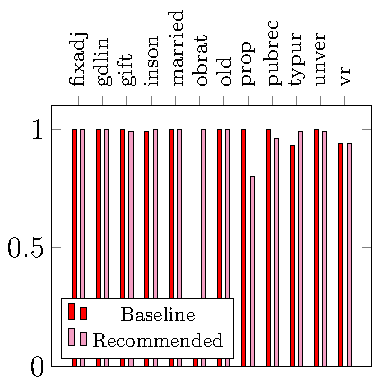
\includegraphics[width=\textwidth]{Figs/econ_cmp-figure0.pdf}
%     \caption{Directionality} \label{fig:econ_cmp_sign_accs}
% \end{subfigure}\hspace{1cm}
% \begin{subfigure}[t]{0.28\textwidth}
%     \centering
%     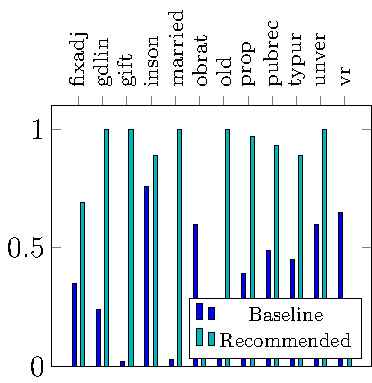
\includegraphics[width=\textwidth]{Figs/econ_cmp-figure1.pdf}
%     \caption{Relevance} \label{fig:econ_cmp_spearmans}
% \end{subfigure}\hspace{1cm}
%  \begin{subfigure}[t]{0.28\textwidth}
%     \centering
%     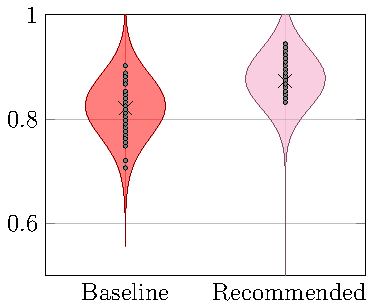
\includegraphics[width=\textwidth]{Figs/econ_cmp-figure2.pdf}
%     \caption{Recall}
%     \label{fig:econ_cmp_recalls}
% \end{subfigure}
% \caption{Improvements due to use of recommended pipeline instead of one without any of our mitigation strategies}\label{fig:econ_cmp}
% \end{figure}


        \begin{figure}[t!]
            \subfloat[SHAP Directionality]{%
                \raisebox{.2cm}{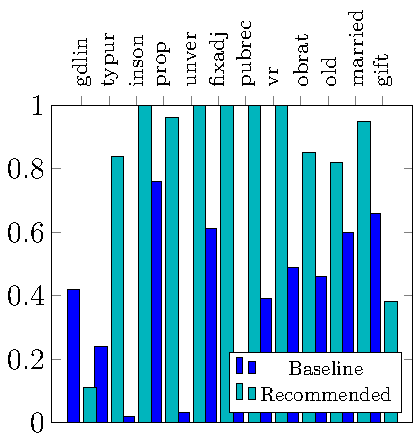
\includegraphics[width=.28\textwidth]{Figures/shap_econ-figure0.pdf}}%
                \label{subfig:econ_shap_sign_accs}%
            }\hspace{1cm}
            \subfloat[SHAP Concordance]{%
                \raisebox{.05cm}{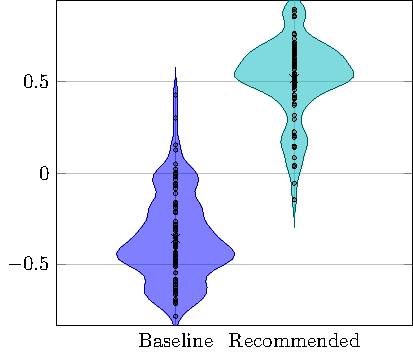
\includegraphics[width=.28\textwidth]{Figures/shap_econ-figure1.pdf}}%
                \label{subfig:econ_shap_spearmans}%
            }\hspace{1cm}
            \subfloat[SHAP Relevance]{%
                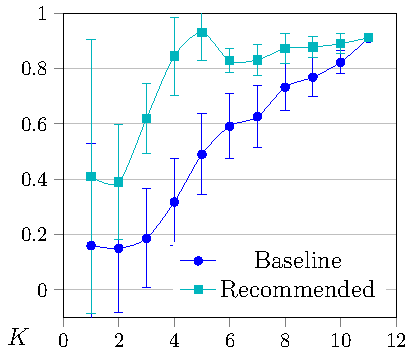
\includegraphics[width=.28\textwidth]{Figures/shap_econ-figure2.pdf}%
                \label{subfig:econ_shap_recalls}%
            }\\
            \subfloat[LIME Directionality]{%
                \raisebox{.2cm}{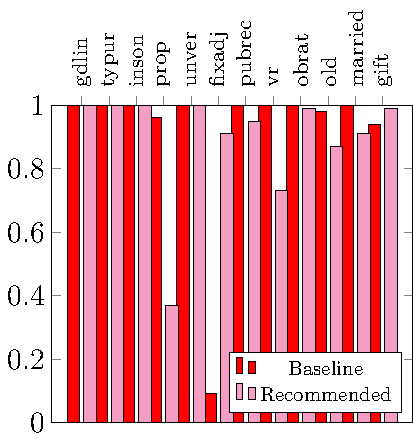
\includegraphics[width=.28\textwidth]{Figures/lime_econ-figure0.pdf}}%
                \label{subfig:econ_lime_sign_accs}%
            }\hspace{1cm}
            \subfloat[LIME Concordance]{%
                \raisebox{.05cm}{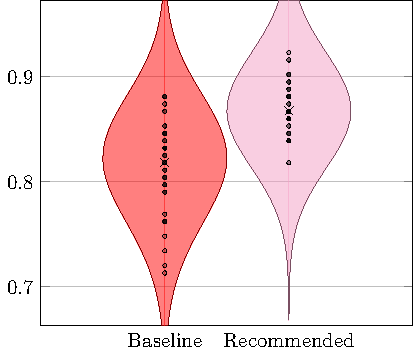
\includegraphics[width=.28\textwidth]{Figures/lime_econ-figure1.pdf}}%
                \label{subfig:econ_lime_spearmans}%
            }\hspace{1cm}
            \subfloat[LIME Relevance]{%
                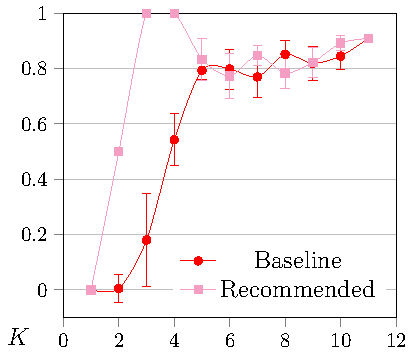
\includegraphics[width=.28\textwidth]{Figures/lime_econ-figure2.pdf}%
                \label{subfig:econ_lime_recalls}%
            }\\
            \caption{Improvements due to use of recommended pipeline instead of one without any of our mitigation strategies}\label{fig:econ_cmp}
        \end{figure}
    %\tw{Figure 12 (f) makes our strategies less convincing. The result looks weird. Did you double check?}



\section{Discussion and Conclusion}
    \label{sec:discussion}
    As post hoc explanations are gaining popularity in business research, we found an alarming trend of using them to make claims about the marginal effects of variables in the data.  However, the validity of this use of post hoc explanations has not been studied in the literature. 
    Our paper is the first effort towards this purpose. 
     In the following sections, we will summarize our findings and give some parting advice for the use of post hoc explainers for obtaining data insights in business research. 
    We also contribute to the business literature by proposing some simple and intuitive mitigation strategies which we found to benefit explainer data-alignment to varying extents.
    %    
    %In this paper we have introduced and investigated issues of misalignment and inconsistency of post hoc explanations. Our thorough literature review uncovered that business researchers using post hoc explanations value data-alignment. Thus we have contributed to the business literature by providing both theoretical and empirical evidence that the two most popular explainers, LIME and SHAP, often produce misaligned explanations. Notably, we proved that SHAP is inherently unsuitable to infer information about $\boldsymbol{\beta}$. %We have also identified various factors that contribute to misalignment and inconsistency. 


    \subsection{Main Findings}
        Our paper contributes several important findings to the use of post hoc explanations in business research.

            First, through an extensive literature review, we found that the use of post hoc explanations to infer information about the data is quite prevalent. In the 150 papers we reviewed, 63 used SHAP or LIME to draw conclusions about the $X\rightarrow Y$ relationship instead of the $\mathcal{M}(X)\rightarrow \hat{Y}$ relationship. Such use deviates from the intended purpose of post hoc explainers; they are designed to explain the machine learning model, not to extract information about the data. Identifying this misuse of post hoc explanations is an important contribution of this paper. Note that while post hoc explanations have been first introduced and widely used in the machine learning community, the issue we discuss in this paper is less of a concern for that community because computer scientists are more interested in explaining the machine learning models. They use post hoc explainers to understand a model's behavior in order to diagnose and debug the model. However, the goal of business researchers is to understand the data and the underlying phenomena, making this issue more pertinent in business research.
        % Using simulated loan application datasets, we produced ground truth application approval mechanisms $\mathcal{G}$ along with NN approximators $\mathcal{M}$ trained on $\mathcal{G}$ and investigated how well popular post hoc explainers could recover the $\boldsymbol{\beta}$ underlying $\mathcal{G}$. This investigation was motivated by the need to assess the utility of post hoc explainers to business researchers and managers. We used our results from the investigation using simulated data to propose a set of mitigations that would worth exploring in practice. Finally, we tested the efficacy of this set of mitigations in a test to see if we could use LIME to reproduce the results of an econometric study of home loan applications. We found that although it was far better to use them than not, the resulting explanations were still imperfect. 

        % When evaluating the ability of the two most popular post hoc explainers, SHAP and LIME, to extract faithful insights from both real and simulated data, we identified the following issues that are cause for concern for researchers interested in $\boldsymbol{\beta}$ estimation problems using post hoc explainers. 

       Second, we provide both theoretical and empirical evidence that SHAP and LIME explanations are, in fact, not data-aligned. In our investigation, we discovered that SHAP and LIME incorrectly represent the signs and relative importance of the marginal effects of the explanatory variables. As shown in Section \ref{sec:causes_of_misalignment}, SHAP and LIME tend to be data-misaligned even in scenarios where they explain an accurate machine learning model trained on data whose features are mutually independent and whose target is derived from a simple linear ground truth model - scenarios which are, in a sense, ideal. This observation suggests a need for caution when interpreting variable relationships based on post hoc explanations. It opens up a dialogue about the complexities of deriving accurate insights from machine learning models via post hoc explainers, contributing to a deeper understanding of their limitations and paving the way for future research in this area. In light of these insights, it may be beneficial for the academic community to revisit prior analyses that have relied heavily on post hoc explanations. This reassessment could ensure that interpretations and conclusions drawn from such models are robust and reflective of their underlying dynamics. Our findings underscore the importance of continuous critical evaluation in the field, especially as we seek to refine our understanding and application of these explanatory tools. 
        
        Third, we find that the reason for lack of data-alignment is different for SHAP and LIME. Achieving data-alignment using SHAP feature importance values is inherently impossible due to the nature of Shapley values. Shapley values represent a feature's contribution to a prediction by considering not only the feature's marginal effect but also its value and the influence of other variables within the explanation process. In the particular case where SHAP explains a linear model, the vector of Shapley values is given by $\boldsymbol{\beta}(\boldsymbol{\xi}-\bar{\mathbf{x}})$, diverging from a direct representation of $\boldsymbol{\beta}$. Moreover, LIME's data-misalignment arises from the mechanics of its default ridge regression approach. Our analysis, supported by Theorem \ref{thm:lime_thm}, indicates that LIME could achieve data-alignment by avoiding the discretization of numerical inputs, sampling many points for its synthetic regression problem, and opting for a significantly larger bandwidth than the default. Yet, even with these adjustments, common properties of real-world data such as correlated variables often hinder the attainment of data-alignment. Nonetheless, it is noteworthy that our evaluations generally reveal \textit{LIME to provide explanations more aligned with the ground truth compared to SHAP}.
 
        
         Finally, we identify several mitigation strategies that show promise in enhancing the data-alignment of explanations across various stages of the explanation pipeline. These strategies, validated through empirical testing, offer significant improvements in aligning explanations more closely with marginal effects. However, it is important to acknowledge that none of the strategies can guarantee complete congruence with marginal effects. This absence of a full guarantee means that while explanations may sometimes align closely with the marginal effects, they cannot reliably do so. Such a scenario potentially restricts the applicability of post hoc explanations for extracting data insights, as users may remain uncertain about the extent to which these explanations accurately mirror the underlying the marginal effect structure. This limitation underscores the need for cautious interpretation and application of post hoc explanation methods in practical scenarios.
        
        
        % \textcolor{red}{what else did we *find*?}

            
        % Second, users must deal with inconsistent explanations because not only do e.g. SHAP and LIME each produce different explanations for the same outcome, but LIME may produce self-contradictory explanations of the same outcome. How to select an explanation(s) from the myriad available from different combinations of accurate black box models, explainers, and explainer hyperparameters is up to the user, but the mitigations suggested in this paper can help users make more informed decisions.%but robustness checks like those presented in this paper can be used to estimate how confident users can be in their selection(s). 



        % stuff re: prescriptive removed
        %Our main finding regarding prescriptive insights is that LIME, SHAP, and DiCE seem to only be of use for actionable recourse a minority of the time. When tasked with generating new application profiles for denied loan applicants, those new application profiles would be approved by $\mathcal{G}$ less than 50\% of the time. %\textcolor{blue}{May need to be removed!! We showed that... DiCE, a counterfactual explainer (as opposed to an attributive one like SHAP and LIME) was always able to produce new application profiles for rejected loan applicants that would lead to approval in our experiments (for a sufficiently small sparsity parameter). }For DiCE, if we restrict the range of feature variations (within one standard deviation) and the number of features allowed to vary, it can only provide prescriptive insights to a small number of denied applicants.
        
    % \subsection{On Mitigation Strategies}
    %     We proposed some intuitive mitigation strategies for the issues of unfaithful and inconsistent explanations. Each of them was effective with respect to at least one of our three metrics. However, none of them were fully effective solutions that would guarantee that practitioners could confidently use LIME or SHAP for $\boldsymbol{\beta}$ estimation and econometric modeling. Thus, we encourage cautionary usage of SHAP and LIME and to consider exploring the usage of our mitigation strategies in efforts to obtain more data-aligned explanations. 
        
    %     Our principal finding regarding faithfulness was that SHAP has no chance at data-alignment unless its Shapley values are normalized by the difference between feature values and feature means. We also found that the most important strategy for increasing the faithfulness of LIME is to disable discretization of numerical features and to make the number of samples and kernel bandwidth it uses for weighted ridge regression large. 
        
    %     %We found some success in increasing the faithfulness of an explanation of a model $\mathcal{M}$ to the ground truth $\mathcal{G}$. As expected, whether $\mathcal{M}$ and $\mathcal{E}$ can correctly predict decisions from $\mathcal{G}$ affects how faithful their explanations are to $\mathcal{G}$. In addition to ensuring low generalization error of $\mathcal{M}$, we also noted that ensuring that $\mathcal{M}$'s training data without correlated or confounded features resulted in remarkably better results than otherwise. However, it is important to note that the explanations were still usually imperfect even though the model and data were ideal. 
    
    %     To combat inconsistency, we proposed techniques to construct aggregate explanations that are better on average than individual explanations. These strategies worked by  averaging feature importance values obtained from explanations obtained from different combinations of models and explainers. The motivation behind these averaging strategies was that they address uncertainty in the choices users need to make by aggregating the many combinations of models and explainers that are the root of the uncertainty. In addition to addressing inconsistency, these strategies resulted in statistically significant improvements in at least directionality, concordance, or relevance. 

    %     In exploring mitigation strategies, we did not find evidence that LIME or SHAP can be used in a way that makes them suitable alternatives to traditional econometric modeling. Although our recommended strategies for SHAP and LIME compared favorably to their associated baselines in a test to reproduce results an actual econometric study of loan approval, they were unable to consistently extract the $\boldsymbol{\beta}$ that the econometricians found. 

%\textcolor{red}{add in the discussion that althgouh we do not know when the explanation aligns with beta, we can identify when they do not: just run  pipeline multiple times with different split of data and different ML model, if the results do not agree, it is a clear sign that the beta-alignment is low}
    
    
    \subsection{On the Use of Post Hoc Explanations}
  We want to emphasize that this paper focuses on the issue of using post hoc explanations to make inferences about the data. We do not explore their use in explaining the machine learning model $\mM$ or its predictions $\mathcal{M}(X)$, which is the primary intended purpose of post hoc explainers. However, it is important to note that even this intended use of post hoc explainers is controversial \citep{garreau2020looking,alvarez18robustness,kumar20shap,jacovi2023diagnosing}. For the scope of this paper, our discussion is solely focused on inferring ground truth information from $\mathcal{G}$ through the explanations for $\mathcal{M}$.

    \subsubsection{General Usage}
      While this paper recommends against using post hoc explanations to make any definite claims about data, it does not mean that post hoc explanations cannot be used at all. Instead of using them as a tool to \textbf{validate} hypotheses and viewing the explanations as evidence, we propose to use post hoc explanations to \textbf{propose} hypotheses that can guide subsequent efforts after they are corroborated.  %\tw{As a preliminary step, researchers can use the level of inconsistency between explanations of models trained on different splits of the data to gauge data-alignment, viewing explanations which do not share common patterns found the collection of explanations as an indication of its implausibility. Following the preliminary step, a
      %An ideal usage of a hypothesis which is deemed to be plausible and interesting would be to empirically validate it through e.g. randomized trials and with collaboration with domain experts. %(1. don't mention inconsistency. just say first use post hoc explanaitons to propose some hypothesis. While they do not guarantee 100\% accuracy, they do offer a high probability of recovering the true effect in the data. Then use follow-up analysis. Don't only say random trials or domain experts. They could use other causal analysis such as (I'll ask Jeffrey about this)}If this were not presently feasible, researchers could at least call on domain experts to validate the hypothesis \citep{donnelly2023rashomon} or do 
     Further analyses are necessary because hypotheses produced by explainers are not guaranteed to be correct and can be performed using tools that are more suited to identification of causal relationships. For example,  \cite{zhang2023can} follow up their search for important features for restaurant survival using SHAP by using causal forests to estimate the treatment effects of those features. Similarly, \cite{hanauer22boosting} use traditional regression as a trusted baseline that they compare SHAP explanations to. 
%      Additionally, as was done in \cite{tang2024china}, plausible post hoc explanations can be used to aid classical regression analyses as a feature selection method. That is, researchers can opt to use only those features which are said to be important by a post hoc explainer(s) in their regressions but should keep in mind that those features may not actually be important to $\mathcal{G}$. \textcolor{red}{I think this is controversial. This is relevance and we said relevance is not 100\%}
    
    
    
% \textbf{How to Make Fruitful use of post hoc Explainers}.
% \cite{Usc paper and the other paper using shap to select features}
%  Model-agnostic post hoc explainers certainly have legitimate use cases, but due to the nature of real business datasets and stakes associated with business problems, we urge the business community to use them with caution and with tempered expectations. The problems of data-misalignment and inconsistency make it difficult for researchers to choose explanations in a principled fashion and ascertain their truth value. Thus, without sufficient domain knowledge or evidence, a researcher can neither believe nor trust the content of a post hoc explanation, nor use it to make inductive inferences. In such a context, the only truly principled view of a post hoc explanation is as a hypothesis. 
 

    
    %Then their explanations can be used as a basis for more rigorous analysis. For example, the treatment effects of features identified as important by the explainers can be estimated using causal forests \citep{zhang2023can}.   
    
        %The outline given in Section \ref{sec:summary_and_strategies} can undoubtably be improved and tailored to user-specific situations, and so is worth expounding. We do so below, and provide additional information that could be useful in different use-cases. 


        %During Prediction stage, before even beginning model development, users should use correlation analysis and any available domain knowledge to identify correlated or colinear features, and then decide whether to drop them from the dataset. % attempt to understand the causal graph associated with their problems and employ statistical tests of unconfoundedness assumptions. With this knowledge, users need to decide whether it is worthwhile to use post hoc explainers instead of randomized experiments. If so, the data should be pre-processed to have the desirable properties we have outlined previously. Domain knowledge and knowledge of the causal graph are useful for this purpose~\citep{zhao2021causal}.% to remove redundant features, causal descendants of a collinear pairs of causally linked features. Confounders should be controlled for if possible.
        %Then, unless users are only interested in explaining a particular black box model, we propose that many be generated and used for explanations. This is due to the Rashomon Effect\citep{semenova22rashomon}, which states that models (interpretable or otherwise) with approximately the same predictive performance will represent different relationships of the input features to the target. In other words, equally good models will have different (possibly conflicting) explanations and interpretations. In the best case, users could leverage explanations entire Rashomon sets of good models from specified model classes and training datasets. We showed that this technique was useful when averaging explanations over a rather small set of NNs with high ROC AUC using LIME explainers which correctly classify the input being explained. Additionally, because we found that the complexity and generalization error of $\mathcal{M}$ was related to post hoc explanation quality and variability, we propose that researchers gather as much training data as feasible.%.qasw11111 and take care not to overfit their models. %Overfitting is especially detrimental because the complexity of the decision boundary of $\mathcal{M}$ contributes to the instability of the explainer. After all, even a perfect explainer for a model which is highly locally nonlinear must be unstable. Thus, needless complexity in a decision boundary due to overfitting could cause an explainer of the decision function to be unstable when it should not be.  

       
        %When starting the explanation stage, users should keep in mind that post hoc explanation can be accidentally misused due to a fundamental misunderstanding of the explainer. For example, \cite{kaur2020interpreting} showed that practitioners misused explanations due to having an incorrect understanding of Shapley values. \cite{jacovi2023diagnosing} also discusses the possibility of users coming away with an incorrect understanding of incomplete explanations because they fill in missing information with their own biases. Users should ensure that they have a complete understanding of how explainers they intend to use work and how their biases may affect their understanding of the explanation. Having done this, we recommend researchers to view post hoc explanations simply as hypotheses and avoid using them to assert novel findings about $\mathcal{G}$ or claiming that they confirm existing hypotheses. 
        
        %As we have discussed, due to the problems of misalignment and inconsistency, researchers should not trust that a single explanation from any explainer applied to any black box model is true unless they can corroborate the explanation. Ideally, explanations would be corroborated using domain knowledge. Otherwise, users could consider comparing the explanations with patterns found in inherently interpretable models or use explainers only for exploratory analyses that are followed up with more rigorous analysis. For example, we recommend that researchers use robustness checks to figure out how confident they can be in the variability of explanations, and select or aggregate explanations from among the large set of explanations created during the robustness checks. 

\subsubsection{Can SHAP be Used as an Alternative to Econometrics Methods?}
    We discuss whether SHAP can be used as an alternative to traditional econometric modeling because this type of usage was a pattern we found in our literature review. That is, researchers were motivated to use SHAP explanations of an ML model to obtain feature importance values because of perceived advantages XAI has over regression analysis. The most commonly cited advantage is that, unlike traditional least squares regression methods, SHAP explanations automatically include nonlinearities and interactions \cite{hanauer22boosting,berger2023supply,srivastava23energy,banulescu2023practical,li24roles}. For example, \cite{berger2023supply} describes their motivation to use SHAP by asserting that SHAP can provide similar economic insights to pooled OLS \emph{and} capture the non-linear impacts of features. \cite{srivastava23energy}, which expresses the desire to use and explain ML models with SHAP in order to find factors driving energy consumption because ML models can ``detect highly complex interactions between drivers of energy consumption," is an example of this. Furthermore, \cite{zhou23consumption} says that XAI methodology is appealing because it does not necessitate ``...the construction of more intermediate variables and complex statistical analysis." Similarly, \cite{banulescu2023practical} are drawn away from logistic regression because it suffers when a large number of predictors are used. \cite{hanauer22boosting} choose not to use traditional linear regression analysis used for fundamental stock analysis and instead explain random forest and XGBoost models because the ML models deal with non-linearities, interactions, and noisy features. \cite{li24roles} makes inferences about bike sharing by explaining their XGBoost model instead of examining the coefficients of their linear regression because the XGBoost had better predictive performance. 

     The fact that SHAP is a local explainer makes its use for obtaining global feature importance unnatural, and this is a shortcoming that SHAP has in comparison to econometric modeling. We found that authors often circumvented SHAP's status as a local explainer by computing the average of the absolute Shapley values over their test set and using the results as measures of global feature importance. \cite{lenaers23rent,maeng23vr,guenther2023useful} are all examples. This obviously comes at the cost of losing any indication of the directionality of impact by features. However, they must do this because the means of signed Shapley values should be 0 due to Equation \ref{eqn:shap_gt}. This is usually the case empirically; \cite{lenaers23rent,maeng23vr,jiang24churn} all show scatter plots of the signed Shapley values of each feature over their dataset and the empirical distributions of the Shapley values are almost always centered at 0. Equation \ref{eqn:shap_gt} implies that the expected absolute Shapley value for feature $X_j$ is proportional to $\beta_j$, but also a function of the mean and standard deviation of $X_j$. So, unless all of the $X_j$ are identically distributed, the expected absolute Shapley values may not be comparable for the sake of relative importance in the same way as the $\beta_j$. In other words, a ranking of the average absolute Shapley values may be different than the ranking of the $\mid \beta_j\mid$.  %For example, if $\beta_1=1$ and $\beta_2=2$ with $X_1\sim\mathcal{N}(\mu_1=100,\sigma_1=1)$ and $X_2\sim \mathcal{N}(\mu_2=0,\sigma_2=\frac{1}{10})$ that are viewed as important in the sense of the effect of a unit increase, the expected absolute Shapley value for $X_1$ is larger than the expected absolute Shapley value of $X_2$ even though $X_2$ is more important than $X_1$ because $\beta_2>\beta_1$:
    % \begin{equation*}
    %     \mathds{E}[\mid \beta_1(X_1-\mu_1)\mid] = \sqrt{\frac{2}{\pi}} > \mathds{E}[\mid \beta_2(X_2-\mu_2)] = \frac{1}{5}\sqrt{\frac{2}{\pi}}
    % \end{equation*}

% \subsection{Using post hoc Explainers on Non-linear Models}    
%     \label{sec:nonlinear} %use taylor series argument
%     \textcolor{blue}{ronilo: I'm worried to talk about other explainers in this section because some of them (SmoothGrad and C-LIME actually do directly approximate the marginal effect), so if I talk about them here the reviewers would criticize us for not using those methods in all of our experiments}
%     %\textcolor{red}{it's a discussion and is not supposed to be so technical. If you can write out the maths, can we just prove it? If you can only do a hand wavy argument, can we avoid using maths or try to use less maths? I also feel it is a little short. We can consider including it in other subsections as a paragraph.}
%     Intuitively, since we demonstrated that SHAP and LIME generally cannot extract the marginal effects from linear models (i.e. the weights of the linear models), it also makes sense that they should not be expected to be able to extract the marginal effects from non-linear models (the gradient at the instance being explained $\nabla \mathcal{M}(\bxi)$). This is the case because $\nabla \mathcal{M}(\bxi)$ is not the estimand of SHAP and LIME. Consider for example cases where $\mathcal{M}$ is a scalar valued real analytic function. We will discuss how LIME and SHAP behave when explaining such $\mathcal{M}$. 
    
%     If $\mathcal{M}$ is linear, then the target in LIME's regression is $\by=\bX \nabla \mathcal{M}(\bxi)$. As LIME is a linear approximator, it will then just output $\nabla \mathcal{M}(\bxi)$ in the best case (as we saw in Theorem \ref{thm:lime_thm}. However, if $\mathcal{M}$ is non-linear, we can see that LIME will generally not be able to extract $\nabla \mathcal{M}(\bxi)$ because $\by \neq \nabla \mathcal{M}(\bxi)$. Instead, $\by$ is given in terms of a power series with higher order terms such as $\nabla^2 \mathcal{M}(\bxi)$. 

%     As shown by \cite{StrumbeljErik2014Epma}, when $\mathcal{M}$ is linear the SHAP coefficients are proportional but not equal to the marginal effects. In general, in the expression of the SHAP value for the $i$th feature in the prediction $\mathcal{M}(\bxi)$, each summand %has a factor $\frac{f(h_\bxi(z'))-f(h_\bxi(z'\setminus i))}{M!}$, where $z'$ is a coalition vector and $M$ is the maximum number of members of a coalition. 
%     includes a factor which is a  rough estimate of $\pdv{\mathcal{M}}{X_i}\big|_{\bxi}$ (a first order difference of $\mathcal{M}$). So, although SHAP values are related to the gradient of $\mathcal{M}$, SHAP is not directly computing or estimating $\nabla \mathcal{M}(\bxi)$.
    
%     %%To illustrate this more concretely, let us assume the settings of Theorem \ref{thm:lime_thm} but allow for $f$ to possibly be a real analytic function (that is, one that can be described locally by a convergent power series). As in Theorem \ref{thm:lime_thm}, suppose we want to explain the prediction of $\mathcal{M}$ at a point $\bxi\in \mathbb{R}^D$ with LIME. Let $\bH$ be the projection matrix produced by LIME's regression, so that $e_{\text{LIME}}(\bxi) = \bH \mathcal{M}(\bX)$ where $\bX$ is a random matrix whose rows are sampled around $\bxi$. If $\mathcal{M}(\bx)=\boldsymbol{\beta}^T\bx$ then $e_{\text{LIME}}(\bxi) = \bH \bX \boldsymbol{\beta}$ and that in the large sample limit, $\bH \bX \rightarrow \bI$ so that $\boldsymbol{\beta}$ is recovered. In the case that $f$ is non-linear, $\by$ is not $\bX \nabla f$. Instead, we consider that, viewing $f$ in a Taylor expansion using a  matrix form of Taylor's theorem, the product $\bH\by$ will generally not be $\bH \bX \nabla f$ and thus $\nabla f$ cannot be recovered. 
%     % the desired output is $\nabla f (\bxi)$ (the gradient of $f$ at $\bxi$). However, using the multivariate form of Taylor's theorem, we have $e_{\text{LIME}}(\bxi) \simeq  \bH(\tilde{\by}_1,\ldots,\tilde{\by}_N)^T$ where $\tilde{\by}_n$ is an approximation of $f(\bx^{(n)})$ for $n=1,\ldots,N$ and %nabla is 1xd
%     % %1x1
%     % %(1,1) + ()(1,D)
%     % \begin{equation*}
%     %     \tilde{\by}_n  = f(\bxi) + (\bx^{(n)} - \bxi)\nabla f(\bxi)^T + \frac{1}{2}(\bx^{(n)} - \bxi) \nabla^2 f(\bxi) (\bx^{(n)} - \bxi)^T
%     % \end{equation*}
%     % % Thus
%     % % % y is N x 1              nxd          dx1           nxd dxd 
%     % % \begin{equation*}
%     % %     \by = f(\bxi)\bI_N + (\bX - \bXi) \nabla f(\xi)^T + \frac{1}{2} (\bX-\bXi) \nabla^2 f(\xi) (\bX - \Xi)
%     % % \end{equation*}
%     % Comparing this to the linear case, we see that if $f(\bx)=\boldsymbol{\beta}^T\bx$ then $\tilde{\by}_n = \boldsymbol{\beta}^T \xi + \boldsymbol{\beta}^T (\bx^{(n)} - \bxi) = f(\bxi) + \nabla f(\bxi)(\bx^{(n)}-\bxi)= \nabla f(\bxi) \bxi + \nabla f(\bxi)(\bx^{(n)}-\bxi)$.
    

    

\subsection{General Concerns About Using Post Hoc Explainers to Get Data Insights}
    % Our concerns about post hoc explainers come from both practical and fundamental issues. The practical issues make obtaining data-aligned explanations from explainer methods which have been developed more difficult and represent challenges that the designers of future methods should meet. The fundamental issues are those that prevent XAI researchers from developing methods that fully address the practical issues.  
    
    % Practical issues have to do with properties of the dataset $(\bX,\by)$,  properties of $\mathcal{M}$ (the Rashomon effect, in particular), properties of $\mathcal{E}$, properties of the ground truth $\mathcal{G}$, and difficulties end-users face when using putative explanations. Regarding the data features, users of post hoc explainers should be concerned if the number of features $D$ is large or if any of the features are correlated. Due to the Rashomon effect, users of post hoc explainers must temper their expectations. 
    
    Although our paper only studies the two post hoc explainers that are most widely used, our concerns about extracting data insights through post hoc explainers are more general. 
    The Rashomon effect \citep{semenova22rashomon,donnelly2023rashomon,rudin2024amazingthingscomehaving} of machine learning models tells us that in any given learning problem there can be an abundance of models with near optimal predictive performance. Each model represents a different hypothesis about the relationship between $\bX$ and $\by$, so the fact that there are many near-optimal hypotheses means that even a perfect explanation of a single model is unlikely to be a true and comprehensive summary of the true relationships hidden in $\mathcal{G}$. Another way to view this problem is to consider the predictions of any machine learning models as the destinations and the decision-making process within a machine learning model is the route that takes an input $\mathbf{x}$ to the output $y$. While many machine learning models can reach the destination (similarly good performance), their routes (the mapping between $\mathbf{x}$ and $y$) may be very different. And there is no guarantee that any particular machine learning captures the true mapping in $\mathcal{G}$.
    
    
    On the other hand, even if a user had access to $\mathcal{G}$ itself, they would still need to be concerned about how they choose and use explainer(s) $\mathcal{E}$. As we illustrated in Section \ref{sec:mitigation_strategies}, it is challenging to decide how to use explainers in a principled manner. %Furthermore, we argued in Section \ref{sec:nonlinear} that if $\mathcal{G}$ is non-linear, the aforementioned issues are made more severe. 
    
    
    
    Explainable machine learning (XAI) is a relatively young field, having begun in the late 2010s as a subfield of machine learning and only recently being explored as a means of explaining ground truths $\mathcal{G}$ rather than models $\mathcal{M}$. A principal challenge consists in the fact that XAI has not yet figured out best practices for extracting information about $\mathcal{G}$ in a way that mitigates the Rashomon effect. After all, the first post hoc explainer that aims to directly mitigate the Rashomon effect (RID \cite{donnelly2023rashomon}) was only published in 2023.
    
    
    % \tw{I think we should remove this paragraph. don't talk about psychology at all in this paper.}
    % Second, the scope of XAI has not yet widened beyond the realms of computer science and machine learning to cover psychology. Consideration of how humans use and process explanations is of paramount importance; a pipeline which overcomes all of the technical issues we have identified in this paper would nevertheless be practically useless if the explanations it generates are incomprehensible. That post hoc explainers give explanations in forms that naturally cohere with human psychology has had deleterious effects. For example, although researchers view SHAP's rigorous game theoretic foundation as a boon, the resulting highly technical meaning of Shapley values ends up being a source of confusion for end users. Human evaluation studies \citep{kaur2020interpreting,passi18trust} have shown that that because data scientists do not fully understand Shapley values, they fill in what they didn't understand about SHAP explanations with their own biases. %This general problem of explainers themselves needing to be explained so that their explanations can be understood is applies to more than just SHAP. For example, 
    
    % Plainly worded natural language explanations are the gold standard for explanations that XAI should strive for, and the current technicality of SHAP and other explainers prevents them from achieving this goal. Whereas a natural language explanation can typically be understood by a native speaker of that language without aid, SHAP and many other explanation methods have to themselves be explained prior to use. Additional examples include Accumulated Local Effect (ALE) plots \citep{apley2020visualizing}, Anchors \citep{ribeiro2018anchors},  Convolutional Neural Network Attention mechanisms \cite{itti1998model}, and counterfactuals \citep{mothilal20dice}, which all fall short of the gold standard because of the technical expertise required for their use.  

    
    
    %Many papers employing human evaluation studies have appeared in recent years demonstrating scenarios in which post hoc explainers were not helpful to users because the explainer was wrong and/or the user misunderstood the explainer~\citep{Krishna2022TheDP,kumar20shap,weerts19human,dieber20assessing,yacoby22judges}
    
    
    %\textcolor{red}{say sth to connect to our paper first and then transition to others. sth like "while LIME and SHAP produce explanations in the form of feature importance, other post hoc explainers ...", to introduce that there are various forms of explanations, which could makes interpretation challenging} . \textcolor{red}{For example... (one example would be helpful to give readers some sense of the concern)} Even SHAP, which produces explanations in the form of feature importance that is relatively easy to understand, still confuses users. 




\subsection{Final Remarks}% and Future Work}
This paper aims to highlight the issue with a rising use of post hoc explanations that we identify as inappropriate. To demonstrate the seriousness of this problem, we show that the misalignment occurs even in the simplest context, where the ground truth $\mathcal{G}$ is linear and features are mutually independent. Even in this simple case, SHAP and LIME produce misaligned explanations. Additionally, explanation quality seems to be limited by feature dimensionality. This being the case expect that in realistic business applications, the data-alignment of post hoc explainers can only be worse that what we have shown in our paper. Real decision processes are often non-linear and involve feature interactions and unobservable features; naturally, these added complexities should reduce the efficacy of SHAP and LIME, making it even more challenging to obtain data-aligned explanations. Given the uncertainty regarding the validity of post hoc explanations, researchers should view them skeptically and consider them as hypotheses rather than definitive claims about reality. 

%\tw{should Figure 13 be updated since we are in the middle of 2024 and there should be more papers in 2024} That is the updated version. 
 
 % When feasible, we advocate for intrinsically interpretable models to be used instead. %When data have unobserved confounders, randomized experiments should be used to identify treatment effects.


    % reword to remove word MISUSE; need to say instead that users get incorrect misunderstanding
    %Throughout this paper, we have shown how and why the use of post hoc explainers could lead to confusion for business researchers and bad decision making for businesses. Our experiments demonstrated SHAP and LIME's inability to produce consistent and faithful explanations. Possible consequences of this include businesses or customers trying to improve upon some outcome, which could waste time and resources by adjusting for an irrelevant feature that LIME or SHAP implied was important, or even worsen the outcome they were trying to improve. On the surface, model-agnostic post hoc explainers are attractive because they are easy to use and applicable to any model with any dataset. However, their propensity toward unfaithful and / or inconsistent explanations decreases their efficacy. Due to the stakes involved with understanding business problems, post hoc explainers should only be used with great caution. 
        

% Acknowledgments here
\section*{Acknowledgements}
We thank Zhongju Zhang, Tat Chan, Shan Huang, and Katherine Ragodos for comments which greatly improved the manuscript. We are grateful to Palle Jorgensen for sharing his wisdom and perspective on the mathematical portions of this work. We would also like to thank the participants of the 2024 Hong Kong Quant Marketing Mini-Conference, BizAI Conference, Production and Operations Management Society (POMS) Conference, Workshop on Information Technologies and Systems (WITS), as well as the participants of the 2023 INFORMS annual meeting and INFORMS Workshop on Data Mining \& Decision Analytics.

% References here (outcomment the appropriate case)

% CASE 1: BiBTeX used to constantly update the references
%   (while the paper is being written).
%\bibliographystyle{informs2014} % outcomment this and next line in Case 1
%\bibliography{<your bib file(s)>} % if more than one, comma separated

% CASE 2: BiBTeX used to generate mypaper.bbl (to be further fine tuned)
%\input{mypaper.bbl} % outcomment this line in Case 2

%If you don't use BiBTex, you can manually itemize references as shown below.


\bibliographystyle{informs2014}
\bibliography{refs}

\newpage

% dimensions finds only 206 but indexes preprints
% scopus finds over 400 but doesn't index preprints
%% preprint not necessary
% need to ensure that the papers are actually explaining a black box
% e.g. tong will anonymize my quotations
% \section*{Appendix A: A Survey of Business Papers that Use SHAP or LIME} \label{apx_sec:lit_review}
    % The appendix contains additional details and experiments. It begins with information about how we conducted our literature review and how we judged papers for inappropriate use of explainers in Appendix Section \ref{apx_sec:lit_review}. We then provide all details relevant for Section \ref{sec:causes_of_misalignment}. First, we give proofs and experimental justification for theoretical claims in Appendix Section \ref{apx_sec:proofs}.
    % Then we detail the experimental designs used in our investigation of correlation and predictive performance in Appendix Section \ref{apx_sec:misalignment_exp_details}. %We expound upon the problem of explainer inconsistency in Appendix Section \ref{apx_sec:inconsistency} using experiments that demonstrate how and why it occurs. 
    % The next part of the Appendix is about our mitigation strategies. Appendix Section \ref{apx_sec:mitigation_details} details our hypothesis testing framework for investigating whether a strategy improves over a baseline pipeline. Appendix Section \ref{apx_sec:additional_mitigations} demonstrates some additional mitigation strategies that we tried that were less effective than the ones in the main body of the paper. Appendix Section \ref{apx_sec:econometric_details} has details about the dataset we used in our econometric case study. Finally, we give the results of a repetition of all experiments in the main body of the paper using a synthetic direct marketing example in Section \ref{apx_sec:marketing}
    
    % \subsection{}
       
        % As part of our literature review process, we cataloged papers at the intersection of business and explainable machine learning. We searched through each of the INFORMS journals and the Web of Science for publications citing at least one of LIME~\citep{ribeiro16lime} or SHAP~\citep{lundberg17shap} and have either ``LIME" or ``SHAP" appear in the body of the article. On Web of Science, the results were filtered by topics related to business, such as management, economics, supply chain \& logistics, operations research \& management science, etc. We also searched on SSRN because business journal papers usually take a few years to get published, so there are many preprints available on SSRN.  We plot the number of papers citing LIME or SHAP by year in Figure \ref{apx_tab:citation_count_graph}. %the following Web of Science topics: transportation, management, economics, supply chain \& logistics, economic theory, and operations research \& management science. Marketing does not appear in the table because Web of Science does not include it as a distinct category among business adjacent fields. Figure \ref{fig:citation_count_graph} shows how the frequency of such papers has increased over time. 
        % Figure \ref{fig:treemap} shows the breakdown of the papers we identified by category. %index any such papers that cited WachterCF~\citep{wachter17wachtercf} or DiCE~\citep{mothilal20dice}.

        % make paragraph or table with prototypical language forms
        % labeled with relevant metric
        % 10 examples of each
        % quotations without citation 
        %We took a close look at these papers and characterized the papers' use of explainers by following two steps. First, we searched for evidence that it was understood that SHAP and LIME explain model outputs, not the data. Next, we searched for problematic language in four forms and recorded quotations of each type (if available). Table \ref{apx_tab:mistakes} provides examples of each language form. The first form was text where the authors either asserted that features which were important to their predictive model(s) per LIME or SHAP were also drivers of their target variable in reality. The second form consisted in recommendations or implications that individuals, groups, managers, or policy-makers should change or guide their behavior on the basis of LIME/SHAP feature importance. In the third form, authors claim that SHAP and LIME explanations are evidence of (or even confirm) an existing hypothesis from prior related work.  The final form was unclear wording that could lead readers to think that the authors were making an assertion of the first form. %Having searched a paper for each form of language, we labeled each paper with 1) why the authors used LIME or SHAP in their paper and 2) whether the paper made an error in using LIME or SHAP (by using language of the first three forms), contained potentially misleading wording, or was error-free. 
        
            % \begin{table}[]
            % \centering
            % \begin{tabular}{l|c}
            % \toprule
            % \textbf{Web of Science Category}         & \textbf{Number of Papers} \\ \hline
            % Operations Research / Management Science & 159                     \\ \hline
            % Management                               & 55                      \\ \hline
            % Economics                                & 47                      \\ \hline
            % Business Finance                         & 42                      \\ \hline
            % Business                                 & 31              \\ \bottomrule
            % \end{tabular}
            % \caption{Number of papers citing either LIME or SHAP that belong to business-adjacent Web of Science categories.}
            % \label{tab:citation_count}
            % \end{table}

        % \begin{figure}[ht]
        %     \centering
        %     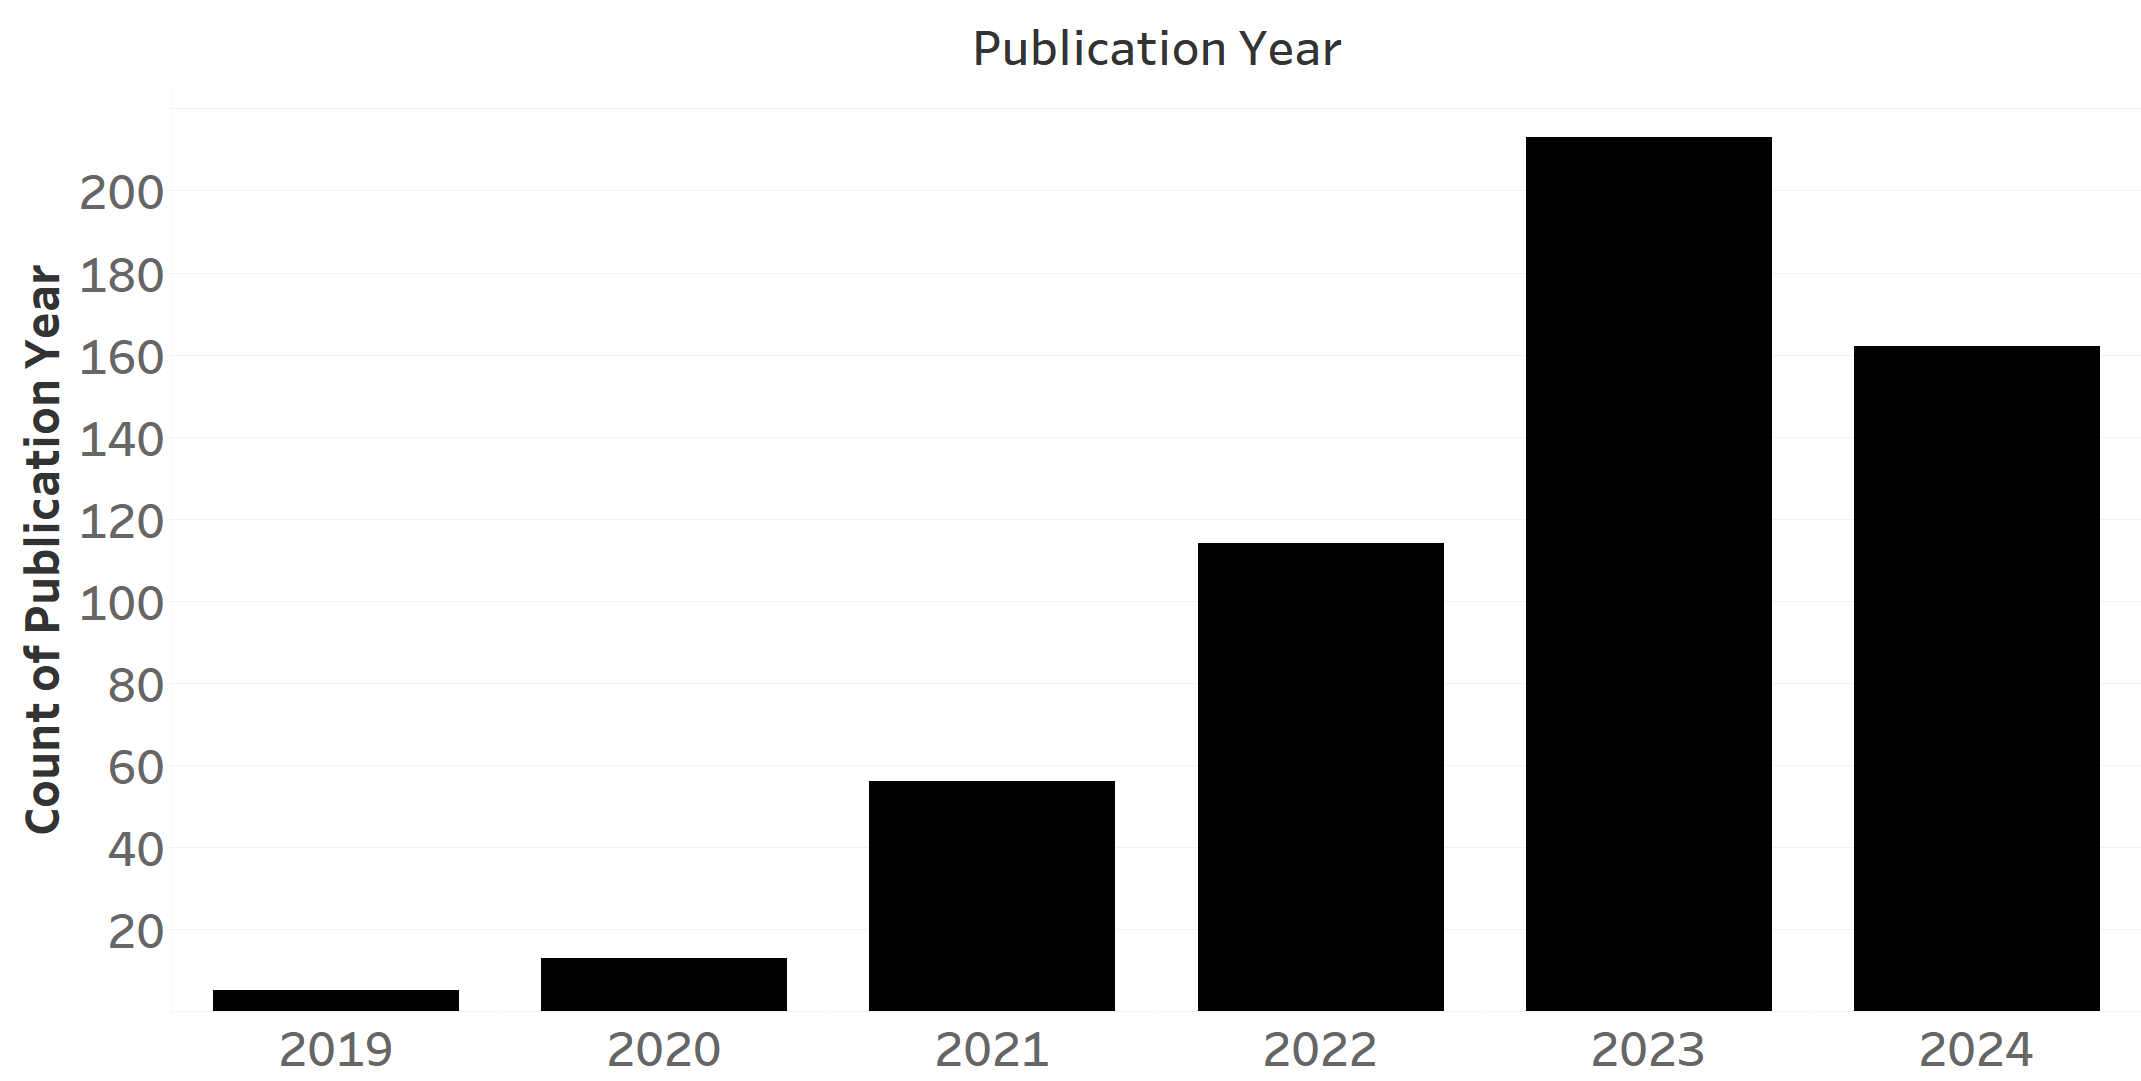
\includegraphics[width=.5\textwidth]{AppendixFigures/citation_count.png}
        %     \caption{Year-by-year breakdown of number of papers citing either LIME or SHAP that belong to business-adjacent Web of Science categories.}
        %     \label{apx_tab:citation_count_graph}
        % \end{figure}
 % We went through each paper to find those that that actually used actually SHAP or LIME to explain a machine learning model instead of just citing them. We stopped at finding 150 such papers.  Out of the 150 papers, 91\% used SHAP and 14\% used LIME.
        % \begin{figure}
        %     \centering
        %     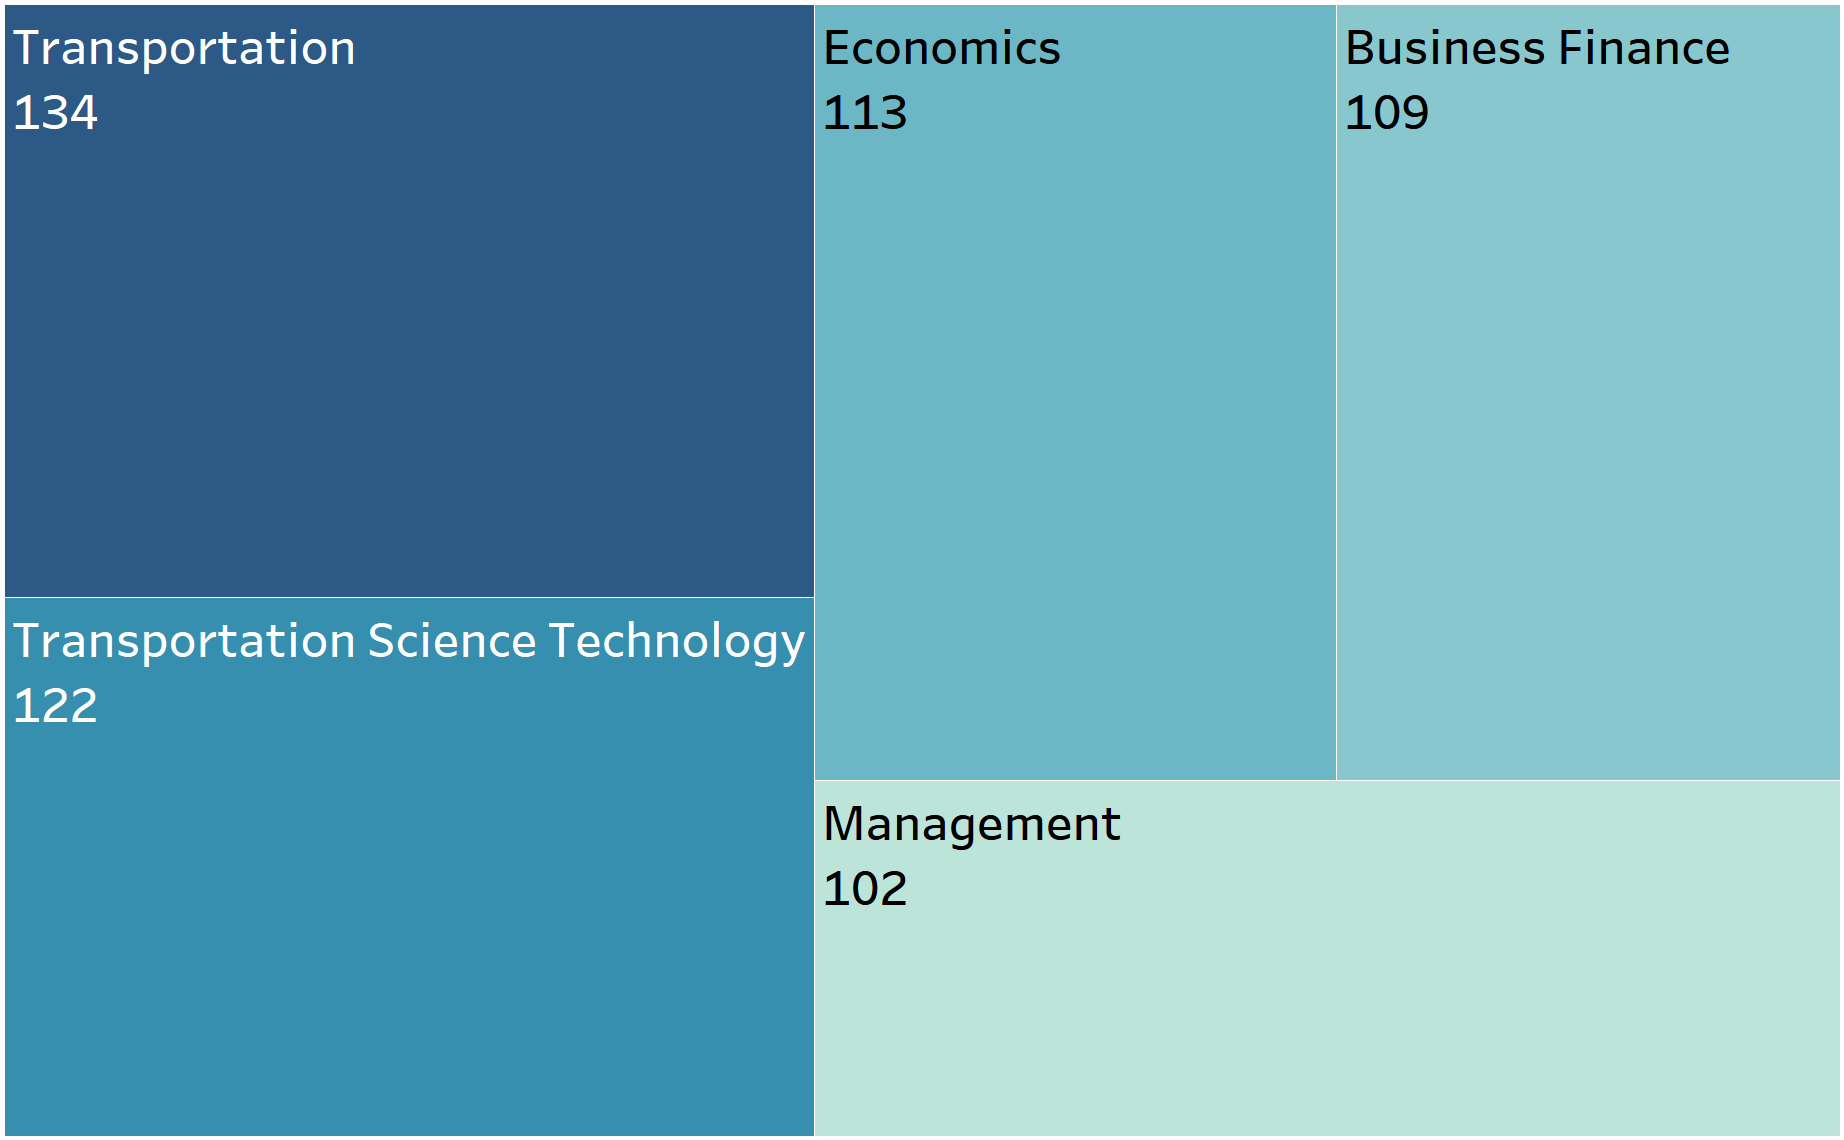
\includegraphics[width=.5\textwidth]{Figs/treemap.png}
        %     \caption{Breakdown of number of papers citing either LIME or SHAP by web of science category.}
        %     \label{tab:treemap}
        % \end{figure}


    % Please add the following required packages to your document preamble:
    % \usepackage{booktabs}
    % \usepackage{lscape}

    % Ambiguous because it's not clear if they mean that the feature is useful for prediction of the target by their model or in reality
%     \begin{landscape}
%    \begin{table}[htbp] 
%     \tiny
%     \caption{Types of Language Used when Interpreting Explanations}
%     \begin{tabu} to 1\linewidth { | X[l] | X[l] | X[l] | X[l] | X[l] | X[l] |}
%        \hline
%        \textbf{Language Form} & \textbf{Example 1} & \textbf{Example 2} & \textbf{Example 3}& \textbf{Example 4} & \textbf{Example 5}\\
%        \hline
%        \textbf{Correct Usage} 
%        & However, as outlined in Rudin (2019), the explanations obtained may not be sufficient for a sensitive decision-making process as the results from these methods can be inaccurate representations of the original relationships and potentially misleading. 
%        & we analyze feature importance metrics to shed light on how machine learning models arrive at their decisions 
%        & We now study the importance of characteristics and their interactions for the performance of gradient boosting and random forests. 
%        & To further understand the inner workings of the language-model classifier, we employ Local Interpretable Model-agnostic Explanations 
%        & The advantage of this method is that for every prediction the RNN model makes, LIME examines nearby instances and their predictions, and tries to ascertain which parameters have influence over the output using instances in the local environment  \\ \hline 
%        \textbf{Extrapolationation}
%        & If there are more blue dots with negative SHAP values and more red dots with positive SHAP values, the
% values of that feature would be positively correlated with the prediction results. In other words, customers with higher scores for this characteristic are more likely to be churners. 
%        & Positive SHAP values indicate that the variable has a facilitative effect on bike-sharing use, while negative values indicate a suppressive effect
%        & Here, SHapley Additive exPlanations (SHAP) systematically uncover the crucial elements that govern guest satisfaction during hotel stays.
%        & XGBoost, is utilized to capture the quantitative associations, and the SHAP (Shapley Addictive exPlanation) model is used to interpret the results from XGBoost. Our results provide empirical support for prior theoretical findings based on mathematical equilibrium models  
%        & Shapley values to understand how various items explain analyst forecasts are generated by utilizing SHAP after XGBoost, when the machine learning model predicts analyst implied ETRs (using the same inputs as predicting actual future ETRs). These Shapley values measure the extent to which various financial
% statement items can explain analyst forecasts \\ \hline
%        \textbf{Advocacy for Recourse}
%        & the method used in this paper has effectively extracted the important influencing variables. On the one hand, it is convenient for investors to quickly evaluate high-polluting enterprises affected by financing, and on the other hand, it can help the government to better promote the transformation of high-polluting enterprises when introducing green credit and green finance
%        & When the product contains quad-core (blue), it has a negative impact on customer choices. This relationship implies that a higher spec is recommended for AP in the smartphone
%        & Since the number of bus stops, bus lines, bike-sharing trips, parking lots and pedestrian shed ratio have high SHAP importance and substantial effects on metro ridership, relevant last-mile transport facilities should be given sufficient attention by transport planners and operators to enhance these access modes to metro stations.
%        & Their SHAP values also raise with the increase of corresponding CV values, revealing that alternative routes with large difference in travel distances, travel speeds or signalized intersection numbers would lead to higher degrees of disequilibrium states at the road network.  
%        & The useful forecasting indicators—higher-order moments—used in this study are of great applied economic importance for helping investors, market participants, and policymakers to forecast the volatility of China’s oil futures more effectively, reduce investment risk, and achieve better returns. \\ \hline
% %        % \textbf{Unclear if Assertion Pertains To $\mathcal{M}$ or $\mathcal{G}$}
% %        &  SHAP can fairly capture the contribution of each predictor and reflect to what extent can each predictor impact the outcome variable
% %        & But credit and the slope of the yield curve, both domestically and globally are consistently the four most
% % important predictors. Together, these results strengthen the view that these key variables are robust indicators for predicting financial crises.
% %        &  According to the feature importance ranking, the top feature may be the potential indicator to trigger financial warning. 
% %        &  These information can be leveraged by the analyst to understand how to reduce the bankruptcy probability of a specific firm or to get insight in which balance sheet fields need to be improved to increase the rating, therefore providing a business instrument to actively manage clients and structured finance deals. 
% %        & By analyzing SHAP values, we identify the credit features that significantly influence borrowers' credit scores, gaining insights into the mechanisms behind these features' impact on personal credit scores. \\ \hline
%        \textbf{OLS Alternative}
%        & Hence, the applied black box algorithm in combination with Shapley values allows to unbox the black box ML approach and provides similar economic insights as provided by pooled OLS
%        & we choose to employ machine learning algorithms instead of traditional econometric techniques. The reason is that machine learning offers the following advantages: (1) Machine learning models can deal with non-linearity and complexity...
%        %, which allows better modelling of complicated relationships between variables; 
%        (2) % Traditional econometric techniques may encounter difficulties when dealing with large datasets due to computational limitations. 
%        Machine learning models are often designed to handle large datasets and can be scaled efficiently; (3) Machine learning models can learn from data without the need for explicit model specification. %They can learn patterns and relationships from the data...% and are therefore well suited for cases where the underlying relationships are not well understood and 
%        (4) Machine learning models can better capture interaction effects between variables...%, allowing a better understanding of how different factors influence each other. 
%        In this way, we then display how key features influence the severity of traffic accidents...% in the early, middle and late stages of the Covid-19 pandemic.
%        & To avoid biased estimates and capture non-linear associations, Light Gradient Boosting Machine (LightGBM) model and SHapley additive explanations (SHAP) model are combined to explore the factors affecting the competitiveness of bike-sharing to underground.
%        & ...conventional linear HAR models may falter. Additionally, the presence of nonlinearity contributing to volatility forecasting among higher-order moments cannot be identified using conventional linear models. However, machine learning (ML) methods have proven to be effective in addressing multicollinearity and accommodating more sophisticated functional forms, enabling the exploration of complex nonlinear relationships among variables 
%        & Machine learning techniques are regarded as a viable alternative to traditional models for traffic forecasting, due to their remarkable ability to capture nonlinearities and exhibit robustness against diverse distributional properties of data. For this reason, machine learning techniques are commonly perceived as a compelling approach for policy and planning analysis \\ \hline
%    \end{tabu}
%    \label{apx_tab:mistakes}
%    \end{table}
%    \end{landscape}
    \section*{Appendix A: Proofs and Numerical Analysis}  
        \label{apx_sec:proofs}    
        The proof for Theorem \ref{thm:lime_thm} as well as justification for Remark \ref{nu_remark} are provided below. We also provide simulation experiments that empirically confirm the the assertions of Remark \ref{nu_remark}. Required lemmas are also proven.
        
        % \subsection{Proofs}
         \subsection{Theorem  
        \ref{thm:lime_thm} Proof}
        \paragraph{Theorem Setting}
        
            To investigate the limitations of LIME, we consider the simple case of explaining a linear function $f:\mathbb{R}^D \rightarrow \mathbb{R}$ such that $f(\mathbf{x}) = \boldsymbol{\beta}^T \mathbf{x}$ at the point $\boldsymbol{\xi}\in \mathbb{R}^D$ (which itself was sampled from $\mathcal{N}(\mathbf{0}_D, \bI_{D\times D})$) using a LIME explainer with the following properties. Suppose that LIME samples random vectors $\{\mathbf{x}^{(n)}\}_{n=1}^N$ with $\mathbf{x}^{(n)} \sim \mathcal{N}(\boldsymbol{\xi},\bI_{D\times D})$ for each $n$ and, given a bandwidth parameter $\nu > 0$, weights their distances to $\boldsymbol{\xi}$ using its default exponential kernel $\pi(\xi,\mathbf{x}) = \exp(-\norm{\boldsymbol{\xi} - \mathbf{x}}_2^2/2\nu^2)$. 
            
        We assume that LIME follows its default settings to solve a ridge regression problem, minimizing the following loss function to obtain a feature importance vector $\hat{\bu}$. 
        \begin{equation*}
            (\mathbf{y} - \mathbf{X}\mathbf{u})^T \mathbf{W}(\mathbf{y} - \mathbf{X}\mathbf{u}) + (\mathbf{u} - \mathbf{u}_0)^T \Delta(\mathbf{u} - \mathbf{u}_0)
        \end{equation*}
        In this loss function, $\mathbf{X} \in \mathbb{R}^{N\times D}$ is a data matrix  whose $n^{th}$ row is $\mathbf{x}^{(n)}$ and $\mathbf{W} \in \mathbb{R}^{N\times N}$ is a diagonal weight matrix for each of the $n=1,\ldots,N$ samples with $w_{nn} = \pi(\boldsymbol{\xi},\mathbf{x}^{(n)}) = \exp(-\norm{\boldsymbol{\xi} - \mathbf{x}^{(n)}}_2^2/2\nu^2)$. The response vector $\mathbf{y}\in \mathbb{R}^N$ is defined pointwise by $y^{(n)} = \boldsymbol{\beta}^T \mathbf{x}^{(n)}$. The ridge penalty parameter $\Delta\in \mathbb{R}^{D\times D}$ has $\Delta = \lambda \bI_{D\times D} \bI_{D\times D}$ so that $\Delta$ represents the ridge penalty with hyperparameter $\lambda=1$. As we shall see, $\lambda$ does not matter because LIME does not set it to scale with $N$. There is also another hyperparameter $\mathbf{u}_0 \in \mathbb{R}^D$ which is the target that $\mathbf{u}$ is to be shrunken toward. By default, it is $\mathbf{0}_D$. 

        In the proof, $n$ will be used to index the $N$ data samples. $i$ and $j$ will be used to index the $D$ features. Individual data samples in the data matrix $\mathbf{X}$ will be represented with superscript notation, e.g., $\mathbf{x}^{(n)}$. Individual features of a sample will be indexed with subscript notation, e.g. $x^{(n)}_j$. We need not refer to whole rows or columns of $\mathbf{W}$, so it will be indexed entry-wise with $w_{nn}$ for $n=1,\ldots,N$. Finally, we will use the Dirac delta function $\delta_{i=j}$, which is 1 when $i=j$ and 0 otherwise. 

            %\begin{theorem*}[\ref{thm:lime_thm}]
            \paragraph{\textbf{Theorem \ref{thm:lime_thm}}}
                %\label{thm:lime_thm}
                Suppose $f:\mathbb{R}^D\rightarrow \mathbb{R}$ that maps $\mathbf{x} \mapsto \boldsymbol{\beta}^T \mathbf{x}$ is explained at a sample $\boldsymbol{\xi}$ drawn from $\mathcal{N}(\mathbf{0}_D, \bI_{D\times D})$ with LIME. Suppose further that LIME does not discretize features and samples i.i.d. data points $\mathbf{x}^{(1)},\ldots,\mathbf{x}^{(N)}$ from $ \mathcal{N}(\boldsymbol{\xi}, \bI_{D\times D})$ for its regression.
                 Then, in the large sample limit, LIME recovers $\boldsymbol{\beta}$.   
            %\end{theorem*}

\noindent \emph{Proof.}
    The main idea underlying the proof is to apply the law of large numbers to a closed form solution to generalized ridge regression. Using the notation previously established, we can write a closed form solution of the regression as
    \begin{equation}
        \label{eq:closed_form}
        \hat{\bu} = (\bX^T \bW \bX + \bI)^{-1}(\bX^T \bW \by)
    \end{equation}
    Here, $\hat{\bu}$ is a point estimate using a single sample of data $\bX$. By simple algebraic manipulation we have, equivalently, 
    \begin{gather*}
         \hat{\bu} =  (\bX^T \bW \bX + \bI)^{-1}(\bX^T \bW \bX) \boldsymbol{\beta}
    \end{gather*}
    Let us define $\hat{\bS} = \frac{1}{N}(\bX^T \bW \bX + \bI) $ and $\hat{\bG} = \frac{1}{N}\bX^T \bW \bX$ so that $\hat{\bu} = \hat{\bS}^{-1}\hat{\bG}\boldsymbol{\beta}$.
    
    We may write $\hat{\bS}$ and $\hat{\bG}$ entry-wise as follows.
    \begin{gather*}
        (\hat{\bS})_{ij} = \frac{1}{N}\sum_{n=1}^N( x_i^{(n)} w_{nn} x_j^{(n)} + \delta_{i=j}) \\
        (\hat{\bG})_{ij} = \frac{1}{N} \sum_{n=1}^N x_i^{(n)} w_{nn} x_j^{(n)} 
    \end{gather*}
    Above, $\delta_{i=j}$ represents the Dirac delta function which is 1 when $i=j$ and 0 otherwise. For fixed $i,j$, the sequence of random variables $x_i^{(1)} w_{11} x_j^{(1)},\ldots,x_i^{(N)} w_{NN} x_j^{(NN)}$ are mutually independent because the samples $x^{(1)},\ldots,x^{(N)}$ are i.i.d. random vectors. 
    By writing the members of the sequence in the form
    \begin{equation*}   
        x_i^{(n)} e^{-\norm{\bxi - \bx^{(n)}}_2^2/2\nu^2} x_j^{(n)}
    \end{equation*}
    we can see that are also identically distributed. %The mean of these terms is finite, as $w_{nn}\in [0,1]$ for all $n=1,\ldots,N$ means that the mean is upper bounded by the square of the largest entry in $\bxi$. 
    %https://math.stackexchange.com/questions/4153550/existence-of-expectation-of-product-of-two-random-variables
    % https://math.stackexchange.com/questions/1043082/bound-the-variance-of-the-product-of-two-random-varables
    By Lemma \ref{finitemean}, the terms have finite means. 
    
    Thus, by the strong law of large numbers, the sample averages $\frac{1}{N}\sum_{n=1}^N x_i^{(n)} w_{nn} x_j^{(n)}+\delta_{i=j}$ converge to $\mathds{E}_{\bx \sim \mathcal{N}(\bxi,\mathbf{1}_{D})}[x_i e^{-\norm{\bxi-\bx}_2^2/2\nu^2}x_j]$ almost everywhere. This means that the ridge adjustment vanishes (converges to a null matrix). Likewise, the averages $\frac{1}{N}\sum_{n=1}^N x_i^{(n)} w_{nn} x_j^{(n)}$ converge to the same value $\mathds{E}_{\bx \sim \mathcal{N}(\bxi,\mathbf{1}_{D})}[x_i e^{-\norm{\bxi-\bx}_2^2/2\nu^2}x_j]$ almost everywhere. Thus, in the large sample limit, $\hat{\bS}$ and $\hat{\bG}$ converge to the same matrix. \textbf{It follows that, in the large sample limit, $\hat{\bS}^{-1}$ and $\hat{\bG}$ cancel each other, and so we expect that $\hat{\bu} \rightarrow \boldsymbol{\beta}$.} That is, $\boldsymbol{\beta}$ is recovered by the regression in spite of the ridge penalty and sample weighting. 
    
    % \qed
    
    
    
   
\begin{lemma}
    \label{finitemean}
   $x_i^{(n)} w_{nn} x_j^{(n)}$ has a finite mean for all $i,j,n$. 
\end{lemma}
    \noindent \emph{Proof.} Fix some $i,j,n$. 
    Since a random variable having finite variance implies that it has a finite mean, it is sufficient to show that $x_i^{(n)} w_{nn} x_j^{(n)}$ has a finite variance. We do this using the fact that, for dependent random variables $A$ and $B$
    \begin{equation}
        \label{varbd}
        \mathrm{Var}(AB) \leq  2\mathrm{Var}(A)\lVert B\rVert_\infty^2+2(\mathbb E[A])^2\mathrm{Var}(B)
    \end{equation}
    When using this inequality, we set $A:=x_i^{(n)} x_j^{(n)}$ and $B:=w_{nn}$.

    We will establish that each term on the RHS of Equation \ref{varbd} is finite in order to show that $\mathrm{Var}(AB)$ is finite. To see that $\mathrm{Var}(A)$ is finite, note that $x_i^{(n)} x_j^{(n)}$ are Chi-square random variables with 1 degree of freedom, which have finite variance. The weights $B=w_{nn}$ are bounded in the interval $(0,1]$, so $\norm{B}_\infty^2$ is finite. Chi-square random variables have finite means, so $\mathds{E}[A]$ is finite. To see that $\mathrm{Var}(B)$ is finite, note again that $B$ is bounded in $(0,1]$. Then $\mathds{E}[B] \leq 1$. As $B$ is bounded, $B^2$ is also bounded. Hence, the variance $\mathrm{Var}(B) = \mathds{E}[B^2]-\mathds{E}[B]^2$ is a subtraction of finite quantities and therefore also finite. Evidently, each term in the RHS of Equation \ref{varbd} is finite, and so $x_i^{(n)} w_{nn} x_j^{(n)}$ has a finite variance. It follows that the mean of $x_i^{(n)} w_{nn} x_j^{(n)}$ is also finite.  \qed

    \begin{lemma}
        \label{norm_bd}
        Under the assumptions of  Theorem \ref{thm:lime_thm}, and given a random  design matrix $\bX \in \mathbb{R}^{N\times D}$,
        \[\norm{(\bX^T \bW \bX + \bI)^{-1}\bX \bW \bX))}_2 \in O\left(\frac{1}{\sigma_{\min}(\bW)^D}\right) \]
    \end{lemma}
    
  \noindent \emph{Proof.} For the sake of brevity we will define $\bA := \bX^T \bW \bX$ and $\bB := \bA + \bI$. To bound $\norm{\bB \bA}_2$, we will begin by bounding $\norm{\bB}$. We employ the following upper bound for the norm of a $D \times D$ matrix's inverse. We use the notation $\sigma_k(\cdot)$ for the $k$th singular value of a matrix and $\sigma_{\min}(\cdot)$ and $\sigma_{\max}(\cdot)$ for the minimum and maximum singular values, respectively. 
  \begin{equation*}
      \norm{\bB}^{-1} \leq \frac{\norm{\bB}^{D-1}}{\mid \mathrm{det}(B)\mid}
  \end{equation*}
  Moreover,
  \begin{gather*}
      \frac{\norm{\bB}^{D-1}}{\mid \mathrm{det}(B)\mid} \leq \frac{\norm{\bA}^{D-1} + 1}{\mid \mathrm{det}(B)\mid} 
      =  \frac{\norm{\bA}^{D-1} + 1}{\prod_k \sigma_k(\bB)} 
      \leq \frac{\norm{\bA}^{D-1} + 1}{\sigma_{\min}(\bB)^D} 
      \leq  \frac{\norm{\bA}^{D-1} + 1}{(\sigma_{\min}(\bA) + 1)^D} 
  \end{gather*}
    The first inequality follows by Cauchy-Schwarz and the facts that  $D>1$ and power functions are monotonic. The last inequality follows from the fact that $\bA$ and $\bI$ are real and symmetric.
    Now, since the spectral norm $\norm{\cdot}_2$ is bounded above by the spectral radius, after applying Cauchy-Schwarz and bounding the denominator we obtain that
    \begin{gather*}
        \frac{\norm{\bA}^{D-1} + 1}{(\sigma_{\min}(\bA) + 1)^D} \leq \frac{\norm{\bX^T}^{D-1}\norm{\bW}^{D-1}\norm{\bX}^{D-1} + 1}{\sigma_{\min}(\bA)^D} \leq \frac{\sigma_{\max}(\bX^T)^{D-1}\sigma_{\max}(\bW)^{D-1}\sigma_{\max}(\bX)^{D-1} + 1}{\sigma_{\min}(\bA)^D}
    \end{gather*}
    We can now bound $\norm{\bB^{-1}\bA}$ using Cauchy-Schwarz as follows.
    \begin{equation*}
        \norm{\bB^{-1}\bA} \leq \frac{\sigma_{\max}(\bX^T)^{D}\sigma_{\max}(\bW)^{D}\sigma_{\max}(\bX)^{D} + \sigma_{\max}(\bX^T)\sigma_{\max}(\bW)\sigma_{\max}(\bX)}{\sigma_{\min}(\bX^T)^{D}\sigma_{\min}(\bW)^{D}\sigma_{\min}(\bX)^{D}}
    \end{equation*}
    Now, since $0<w_{nn}\leq 1$ for all $n=1,\ldots,N$, and since singular values are invariant under transposition, we can give the following upper bound which should be viewed as a function of $\sigma_{\min}(\bW)$ since we assumed that $\bX$ is fixed. 
    % \begin{equation*}
    %     \norm{\bB^{-1}\bA} \leq \left(\frac{\sigma_{\max}(\bX^T)^{D}\sigma_{\max}(\bX)^{D} + \sigma_{\max}(\bX^T)\sigma_{\max}(\bX)}{\sigma_{\min}(\bX^T)^{D}\sigma_{\min}(\bX)^{D}}\right) \frac{1}{\sigma_{\min}(\bW)^D}
    % \end{equation*}
    % Since singular values are invariant under tranpsosition, we can simplify this into
    \begin{equation*}
        \norm{\bB^{-1}\bA} \leq \left(\frac{\sigma_{\max}(\bX)^{2D} + \sigma_{\max}(\bX)^2}{\sigma_{\min}(\bX)^{2D}}\right) \frac{1}{\sigma_{\min}(\bW)^D}
    \end{equation*}

\begin{remark2}[Connection to condition numbers]
    \label{condition_number_remark}
    $\norm{\bB^{-1}\bA}$ may be made larger when $\bW$ is ill-conditioned.
\end{remark2}
        Recall that the condition number $\kappa(\cdot)\geq 1$ induced by the spectral norm of a matrix is the ratio of its largest and smallest singular values. The bound of Lemma \ref{norm_bd} can be written in terms of condition numbers. By writing it in this form, it can be inferred that $\norm{\bB^{-1}\bA}$ is made larger when $\bW$ is ill-conditioned. 
    \begin{equation*}
        \norm{\bB^{-1}\bA} \leq \left(\kappa(\bX)^{2D} + \frac{\kappa(\bX)^2}{\sigma_{\min}(\bX)^{2D-2}}\right) \kappa(\bW)^D 
    \end{equation*}
    The ill-conditioning of $\bW$ occurs when $\bW$ is close to being singular, which can happen when $\nu$ is near $0$ since this would cause all entries of $\bW$ to be either 0 or close to it. 


    \subsection{Details on Remark \ref{nu_remark}}
                Remark \ref{nu_remark} suggested that, fixing a design matrix $\bX$ consisting of $N$ samples, then if 1) $\nu$ is too small then each of the coefficients of $\hat{\bu}$ will be near $0$ and 2) making $\nu$ very large may yield a better  approximation of $\boldsymbol{\beta}$. Both of these statements have to do with the construction of the weight matrix $\bW$ using a given $\bX$. 

                Recalling that $\hat{\bu}=(\bX^T \bW \bX+\bI)^{-1}\bX^T \bW \bX \boldsymbol{\beta}$ and that, by Theorem \ref{thm:lime_thm} $\hat{\bu}$ tends to $\boldsymbol{\beta}$ in the large sample limit, we can infer that it is desirable for $(\bX^T \bW \bX+\bI)^{-1}\bX^T \bW \bX$ to be near the identity matrix and, therefore, to have norm $1$. Lemma \ref{norm_bd} gives an upper bound on $\norm{(\bX^T \bW \bX+\bI)^{-1}\bX^T \bW \bX}$, so we can use it to investigate what makes this upper bound large. By analyzing $\norm{(\bX^T \bW \bX+\bI)^{-1}\bX^T \bW \bX}$, we can get a rough estimate of how much $\boldsymbol{\beta}$ is distorted. % and possibly more distant from the identity matrix.
                
                We can deduce from the bound given in Lemma \ref{norm_bd} that setting $\nu$ too small makes it possible for $\norm{\bB^{-1}\bA}$ to be large. This is because $\sigma_{\min}(\bW)$ is just $\min_{n=1,\ldots,N} w_{nn}=\min_{n=1,\ldots,N} e^{-\norm{x^{(n)}-\bxi}_2^2/2\nu^2}$ and smaller $\nu$ increases the decay rate of the $w_{nn}$, leading to $\frac{1}{\sigma_{\min}(\bW)^D}$ being very large. On the other hand, since in the context of Lemma \ref{norm_bd} $\bX$ is fixed, larger values of $\nu$ make $\frac{1}{\sigma_{\min}(\bW)^D}$ closer to $1$ and therefore lead to smaller upper bounds for $\norm{\bB^{-1}\bA}$.

                % https://mathoverflow.net/questions/353085/anti-concentration-inequalities-lower-bound-on-realized-second-moment
                To see this more concretely, suppose that a random design matrix $\bX$ with rows sampled from $\mathcal{N}(\mathbf{0}_{D}, \bI_{D\times D})$ is fixed. Furthermore, assume that each row has $\norm{\bx^{(n)}} \leq 1$. Then, we can use the anti-concentration of the norms of the rows $\bx^{(n)}$ to show that when $\nu$ is too small, all values in $\bW$ will be smaller than a value $\epsilon > 0$. Simple computations show that $w_{nn} < \epsilon$ when $\norm{\bx^{(n)}} > t:= \sqrt{2}\sqrt{-\log(\epsilon)/\nu^2}$. If we assume that $t\leq \mathds{E}[\norm{\bx}^{(n)}]$, and by extension impose the restriction $\nu \geq \sqrt{2}\sqrt{-\log(\epsilon)/D}$, we may use an application of the Azuma-Hoeffding inequality \citep{hoeffding1994probability} to estimate the probability that $\norm{\bx^{(n)}}$ is sufficiently large that $w_{nn} < \epsilon$. 
                \begin{equation*}
                    \mathds{P}[\norm{\bx^{(n)}} > t] \geq 1 - \frac{1}{2D}\exp(-2\sqrt{2}\sqrt{-\log(\epsilon)/\nu^2}-2\sqrt{D})
                \end{equation*}
                If, for example $D=100$, $\epsilon=\frac{1}{1000}$, and $\nu$ takes on the smallest value for the inequality to be used (about $.38$), then $\mathds{P}[\norm{\bx^{(n)}} > t]=1$. That is, $w_{nn}<\epsilon$  almost surely.


            %https://arxiv.org/abs/0810.0800
            % , given $\nu < 1$ we can see from the concentration of a gaussian vector that 
            %fixing eps > 0, wnn will be less than epsilon whenever $\norm{x-xi}_2 > sqrt(-2log(eps)/nu^2)$. Then, setting t =   (-2log(eps)/nu^2)^1/4, we see from a subgaussian tail bound that
            %P[\norm{x-xi}_2 > t] > 
            
        \subsection*{Insights From Theoretical Results}
            \begin{itemize}
                \item Although explanations using discretized features may be more easily interpretable, they make the explanations less data-aligned
                \item Users should generally opt to set $N$ to be large 
                \item Users should generally set $\nu$ to be large, otherwise the LIME coefficients may be become zero
                %\item LIME becomes more unfaithful as the number of features $d$ grows. 
                \item The ridge penalty matters only when $\lambda \in O(N)$
            \end{itemize}
    
            \subsection*{Simulation Experiments}
                \label{apx_sec:simulation_experiments}
                We provide simulations to test the assertions of Theorem \ref{thm:lime_thm} and Remark \ref{nu_remark} experimentally. We adopt the settings of Theorem \ref{thm:lime_thm} and experimentally test the roles of $N$, $\nu$ on the convergence of weighted ridge regression using LIME's exponential kernel and the ridge penalty set to $\Delta=1$.% In the second simulation, we use implementation of LIME by its authors and our loan dataset. In this simulation we investigate how the discretization setting affects the actual LIME implementation. In particular, we investigate the ratios $e_{\text{LIME}}(x^{(i)}_j)/\beta_j$. 
    

                
                \paragraph{Role of $\nu$ and $N$ on convergence}
                    We give empirical confirmation of the assertions of our theoretical results and show the experimental results in Figure \ref{apx_fig:nu_N_convergence}. To do this, we create ten random design matrices $\mathbf{X}$ for each combination of $N=10,100,1000,10000,1000000$ rows and $D=5,10,100$ columns. For each of these matrices, we compute $\norm{\bB^{-1}\bA - \mathbf{I}}$ using each of $\nu=.1,1,10,10000$. We report the mean value of $\norm{\bB^{-1}\bA - \mathbf{I}}$ as $N$ is varied.


                    Figure \ref{apx_fig:nu_N_convergence} is a log-log plot of dimension versus the distance $\norm{\bB^{-1}\bA - \mathbf{I}}$. It shows that small $\nu$ leads to slower convergence and larger $\nu$ leads to faster convergence. It also shows that increasing $N$ generally leads to $\norm{\bB^{-1}\bA - \bI}$ being smaller. That the curves are approximately linear indicates the presence of a power law relationship. These results constitute supporting evidence for our claim that $\nu$ and $N$ should be set to large values. In particular, it is advantageous to set them to be larger than their defaults of $\nu=.75\sqrt{D}$ and $N=1000$. 
                    
                    % It shows that, for not too small $\nu$, $\norm{\bB^{-1}\bA - \mathbf{I}}$ converges to $1$, not needing $n$ to be unreasonably large. For example, it seems to be sufficient to use the default settings of $\nu = .75\sqrt{d}$ and $n=1000$. However, it is apparent from Figure \ref{apx_fig:nu_N_convergence} that the largest settings $nu=10000$ gives an advantage for smaller $n$.  

                    % Figure \ref{apx_fig:nu_D_convergence} illustrates the relations of $d$ and $\nu$ with $\norm{\bB^{-1}\bA - \mathbf{I}}$. It shows that larger $\nu$ are associated with smaller $\norm{\bB^{-1}\bA - \mathbf{I}}$ and larger $d$ are associated with larger $\norm{\bB^{-1}\bA - \mathbf{I}}$. This implies that, while increasing $\nu$ is beneficial to LIME's fidelity, larger $d$ make attaining higher fidelity more difficult (especially for small $\nu$). This backs up the results shown in Figure \ref{fig:lime_shap_vary_d}, that is, that increasing $d$ is generally associated with lower data-alignment. 
    
                % \begin{figure}[ht!]
                % \centering
                %     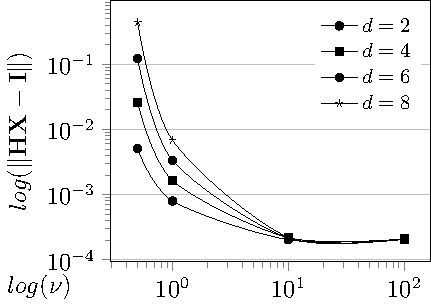
\includegraphics[height=.2\textwidth]{AppendixFigures/apx_lime_conv-figure0.pdf}%{Figures/fig21.pdf}
                %     \caption{Role of $\nu,n$ on $\norm{\mathbf{H}\mathbf{X} - \mathbf{I}}$, with $d=4$.}
                %     \label{apx_fig:nu_N_convergence}
                % \end{figure}

                % %\paragraph{Role of $d$ on convergence}
    
                % \begin{figure}[ht!]
                % \centering
                %     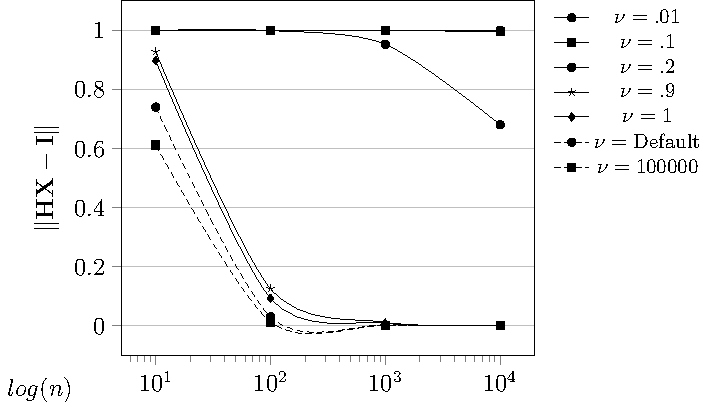
\includegraphics[height=.2\textwidth]{AppendixFigures/apx_lime_conv-figure1.pdf}%{Figures/fig21.pdf}
                %     \caption{Role of $d$ on $\norm{\mathbf{H}\mathbf{X} - \mathbf{I}}$ with $n=50000$}
                %     \label{apx_fig:nu_D_convergence}
                % \end{figure}

                \begin{figure}[ht!]
                \centering
                    %\begin{subfigure}{}
                    \centering
                    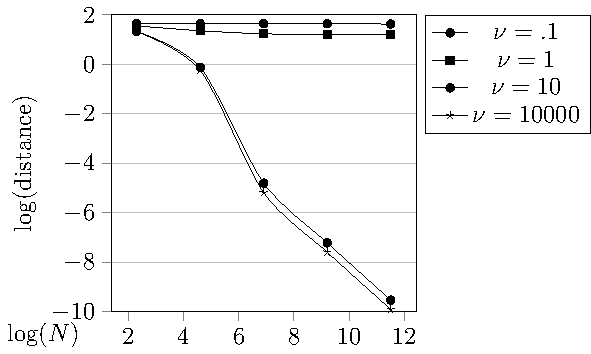
\includegraphics[width=.5\textwidth]{Figures/new_apx_lime_conv.pdf}%{Figures/fig21.pdf}
                    \caption{Log-log plot of the how $\nu,N$ influence $\norm{\bB^{-1}\bA - \mathbf{I}}$. }
                    \label{apx_fig:nu_N_convergence}
                    %\end{subfigure}%
                    % \hspace{3cm}
                    % \begin{subfigure}{.2\textwidth}
                    % \centering
                    % %\fbox{\includegraphics[width=\textwidth,trim=0 10 70 70 mm, clip=true]{Figures/fig21.pdf}}%{Final_Figures/fig20.png}
                    % 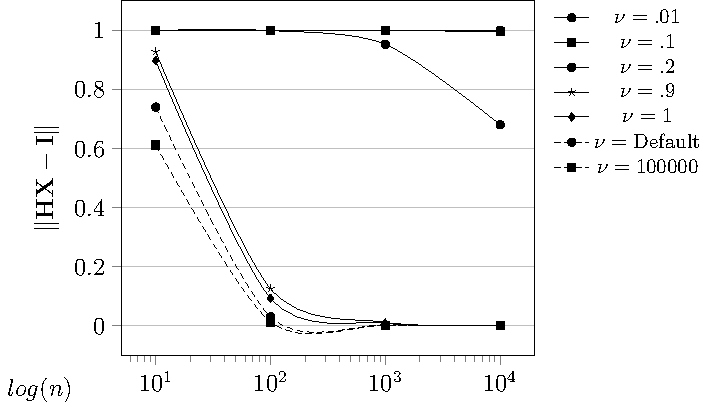
\includegraphics[height=\textwidth]{AppendixFigures/apx_lime_conv-figure1.pdf}%{Figures/fig21.pdf}
                    % \caption{Role of $d$ on $\norm{\bB^{-1}\bA - \mathbf{I}}$ with $n=50000$}
                    % \label{apx_fig:nu_D_convergence}
                    % \end{subfigure}
                \end{figure}
    %             \paragraph{Upper Bounds on $\norm{ (\mathbf{X}^T \mathbf{W} \mathbf{X} + \mathbf{I})^{-1}\mathbf{X}^T\mathbf{W}\mathbf{X}}_2$}
    %                 We show in Figure \ref{apx_fig:nu_N_convergence} that, except when $\nu$ is too small ($\nu<.2$), increasing the number of samples $n$ generally nets a significant decrease in an upper bound for the error of LIME's ridge problem. We use the condition number of  $\norm{ (\mathbf{X}^T \mathbf{W} \mathbf{X} + \mathbf{I})^{-1}\mathbf{X}^T\mathbf{W}\mathbf{X}}_2$ as an upper bound.     
                
    %                 \begin{figure}[ht!]
    %                 \centering
    %                     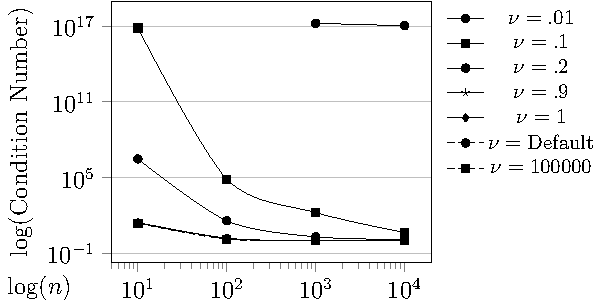
\includegraphics[height=.2\textwidth]{AppendixFigures/apx_lime_conv-figure2.pdf}%{Figures/fig21.pdf}
    %                     \caption{Role of $\nu,n$ on upper bound of $\norm{\mathbf{H}\mathbf{X} - \mathbf{I}}$}
    %                     \label{apx_fig:nu_N_convergence}
    %                 \end{figure}

    
    %             \paragraph{Role of Discretization}
    %                 We provide evidence of our claim that users should not let LIME discretize numerical features if recovery of the marginal effects is their aim by comparing LIME explainers with and without discretization. For our comparison, we use LIME with and without discretization to explain a linear regressor $f(x) = .05 + .05x_1+ .2x_2+ .8x_3 -.5x_4 +x_5$ with $x_i \sim \mathcal{N}(0,1)$ for all $i$. $\nu$ is set to the default value. We pick 100 test set instances and explain each two sets of 100 LIME explainers. The first set of LIME explainers do not use feature discretization while the second set does. The $i^{th}$ explainer has its random seed set to $n$ in both sets. 

    %             %As we claimed in Section 3, the LIME explainers with no feature discretization generally have $C_i$ closer to $1$ than the LIME explainers with discretization. The difference is especially stark with $C_{1}$, which is always 1 with no discretization and between -10 and 20 with discretization. Note that when $C_i$ is negative, LIME has misidenified how feature $i$ impacts the output of $f$. Moreover, in accordance with Theorem 1 and \citep{garreau20theoretical}, we see that $C_i$ can differ significantly across $i$, indicating that $e(x_j)$ is not directly proportional to $\boldsymbol{\beta}$ regardless of whether discretization is used. 

    %             For each set of explainers, we plot the ratios $C_i:= e(x_j)_i/\beta_i$ for $i=1,\ldots,5$ in Figure \ref{apx_fig:c_demo}. The most striking result is that all $C_j$ are centered around $\frac{1}{3}$ and contained in $[-1,1]$ when discretization is turned off, but $C_1$ takes on values in $[-10,10]$ with a mean of $\sim 3.70$ and $C_2,C_3,C_4,C_5$ have respective means of $.52$, $.06$, $.03$, and $-.001$ when discretization is allowed. Thus, when discretization is allowed, LIME may distort the $\beta_j$ more and have severe inconsistency between how much distortion is present across each $j$. That the $C_j$ have nearly identical means when discretization is not used indicates that, on average, the correct rankings of the $X_j$ are preserved in the $e(x_j)_i$. The $C_j$ being very different when discretization is used indicates that such LIME rankings would (almost) never match the ground truth ranking. 
                
    %             %use fbox to tailor crop
    %             \begin{figure}[ht!]
    %             \centering
    %                 \begin{subfigure}{.28\textwidth}
    %                 \centering
    %                 %\fbox{\includegraphics[width=\textwidth,trim=0 10 70 70 mm, clip=true]{Figures/fig21.pdf}}%{Final_Figures/fig20.png}
    %                 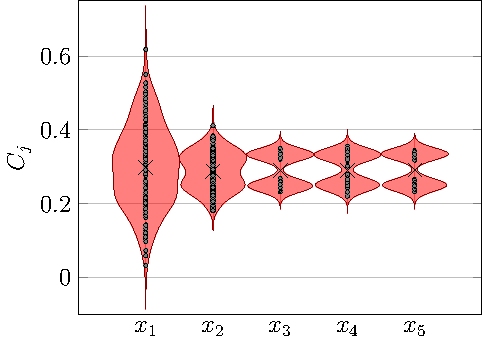
\includegraphics[width=\textwidth]{AppendixFigures/apx_lime_proportionality-figure0.pdf}%{Figures/fig21.pdf}
    %                 \caption{No discretization}
    %                 \label{apx_fig:empirical_c}
    %                 \end{subfigure}%
    %                 \hspace{3cm}
    %                 \begin{subfigure}{.28\textwidth}
    %                 \centering
    %                 %\fbox{\includegraphics[width=\textwidth,trim=0 10 70 70 mm, clip=true]{Figures/fig21.pdf}}%{Final_Figures/fig20.png}
    %                 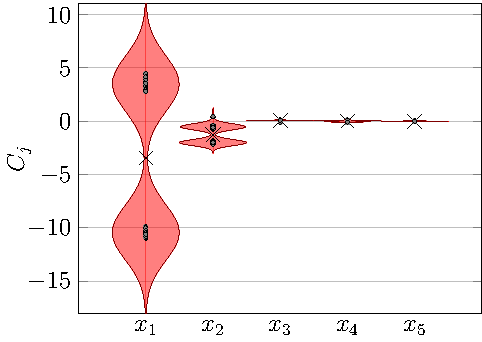
\includegraphics[width=\textwidth]{AppendixFigures/apx_lime_proportionality-figure1.pdf}%{Figures/fig21.pdf}
    %                 \caption{Discretization allowed}
    %                 \label{apx_fig:theoretical_cs}
    %                 \end{subfigure}%
    %             \caption{Empirical $C_j$ for 100 applicants from 100 LIMEs with/without discretization, and all other parameters set to the defaults.}
    %             \label{apx_fig:c_demo}
    %             \end{figure}
    

    


    
    
  
    
    
    % % \section*{Appendix C: Details and Additional Experiments for Section \ref{sec:causes_of_misalignment}}
    % %     \label{apx_sec:misalignment_exp_details}
    % %     This section provides additional experiments for %and details about how the datasets were generated in 
    % %     Section \ref{sec:causes_of_misalignment}, where we discuss causes of misalignment.
    %     %as well as additional experiments that show how correlation and confounding can affect interpretations of post hoc explanations. Table \ref{tab:simulated_variations} documents what features are used in each experiment. 
    
    %         % \begin{table}[]
    %         % % determine target width of combined cols 2 and 3:
    %         % \settowidth\mylenA{Correlated \\ Features} 
    %         % % determine usable width of cols 2 and 3:
    %         % \setlength\mylenB{(\mylenA-3\tabcolsep)/3}
    %         % \centering
    %         % \begin{tabular}{|c|*{3}{wc{\mylenB}|}*{3}{wc{\mylenB}|}*{3}{wc{\mylenB}|}}
    %         % \hline
    %         % \textbf{Experiment} & \multicolumn{3}{c|}{\makecell{\textbf{Correlated} \\ \textbf{Features}}} & \multicolumn{3}{c|}{\makecell{\textbf{Unobserved} \\ \textbf{Confounder}}} & \multicolumn{3}{c|}{\makecell{\textbf{Observed} \\  \textbf{Confounder}}} \\ \hline
    %         % \textbf{Feature} & \textbf{$\mathcal{G^*}$} & \textbf{$\mathcal{G_{\text{effect}}}$} & \textbf{$\mathcal{M}$}             
    %         % &   \textbf{$P_1$} & \textbf{$\mathcal{G_{\text{effect}}}$} & \textbf{$\mathcal{M}$}              & \textbf{$P_1$} & \textbf{$\mathcal{G_{\text{effect}}}$}             & \textbf{$\mathcal{M}$}             \\ \hline
    %         % Age              & \checkmark& \textcolor{red}{\checkmark}    & \checkmark                                                            & \checkmark  & \checkmark    & \checkmark                               & \checkmark& \checkmark   & \checkmark                               \\ \hline
    %         % Sex              & \checkmark& \checkmark & \checkmark   & \checkmark  & \checkmark   & \checkmark                                & \checkmark& \checkmark & \checkmark                                 \\ \hline
    %         % Inquiries        & \checkmark& \checkmark  & \checkmark &  \checkmark     &\multicolumn{1}{c|}{\checkmark}        & \checkmark & \checkmark & \textcolor{red}{\checkmark}    & \checkmark                     \\ \hline
    %         % Cosigner         & \checkmark& \checkmark   & \checkmark                                                              & \checkmark  & \checkmark                                   & \checkmark& \checkmark & \checkmark  &\multicolumn{1}{c|}{\checkmark}                                \\ \hline
    %         % Utilization      & \checkmark& \checkmark  & \checkmark                                                                 & \checkmark  & \checkmark   & \checkmark                                & \checkmark& \textcolor{red}{\checkmark}  & \checkmark                                \\ \hline
    %         % Credit Score     & \checkmark& \textcolor{red}{\checkmark} & \checkmark                                 &                               & \checkmark  & \checkmark  & \checkmark & \textcolor{red}{\checkmark}  & \checkmark                                \\ \hline
    %         % %Social Support   & \multicolumn{1}{c|}{}    & \multicolumn{1}{c|}{}                               &                                    &  \multicolumn{1}{c|}{}  & \multicolumn{1}{c|}{\textcolor{red}{\checkmark}} & \multicolumn{1}{c|}{} & \multicolumn{1}{c|}{}                                 &\multicolumn{1}{c|}{}             &\multicolumn{1}{c|}{}                      \\ \hline
    %         % Income & \multicolumn{1}{c|}{}    & \multicolumn{1}{c|}{}      &     & \multicolumn{1}{c|}{}                                       & \multicolumn{1}{c|}{\textcolor{red}{\checkmark}} & \multicolumn{1}{c|}{} & \multicolumn{1}{c|}{}                                  &\multicolumn{1}{c|}{}  &\multicolumn{1}{c|}{}                                 \\ \hline
    %         % \end{tabular}
    %         % \caption{Table indicating whether the ground truth models $P_1$ and $\mathcal{G}_{\text{effect}}$ use each feature  and whether $\mathcal{M}$ has access to each feature in data produced by ground truth models using them in each experiment. Features which are correlated in $\mathcal{G}_{\text{effect}}$ are marked red.} 
    %         % \label{tab:simulated_variations}
    %         % \end{table}
            
      
        
       
        
    %     \subsubsection{Correlated Features}
    %         We showed that, when explaining predictions of models with similar predictive performance trained on two similar datasets that differ by virtue of their features being mutually independent (or not), the explanations of the model trained on the data with mutually independent features were more data aligned. One of the differences between the two datasets was that in the original, being married increased the chance that an applicant had a cosigner, while in the variant they were independent. In this experiment, we will show how an example of how ``Married" influencing ``Cosigner", a more important feature for loan approval, is associated with lower data-alignment of explanations with respect to ``Married" in particular.
        
    %         Figure \ref{apx_fig:marital_sign_accs} shows bar plots of directionality for the ``Married" feature by SHAP and LIME before and after making ``Cosigner" depend on ``Married." The bar plots show that the addition of dependencies between features is associated with a loss of the ability to give ``Married" the correct sign for both SHAP and LIME. Additionally, Figure \ref{apx_fig:marital_rank_diff} shows the distributions of the absolute differences between the given and correct rank for ``Married" before and after addition of correlated features. We see that for both SHAP and LIME, the average ranking error for ``Married" is much smaller when the features are mutually independent than otherwise. These results suggest that it may be more difficult for explainers to extract correct  information about interdependent features.
    %         \begin{figure}[ht!]
    %             \centering
    %             \begin{subfigure}{.28\textwidth}
    %               \centering
    %               \captionsetup{justification=centering}
    %               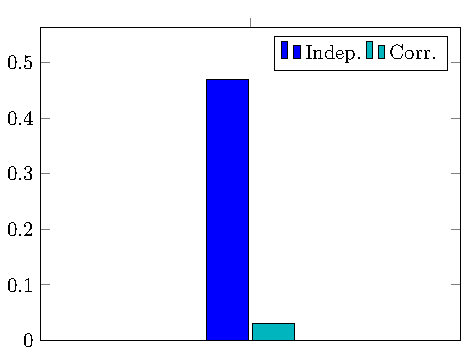
\includegraphics[width=\textwidth]{AppendixFigures/apx_marital-figure1.pdf}%{Figures/fig_age_col.pdf}%{Figures/lime_spearman_colinear.png}
    %                             %\includegraphics[width=.9\linewidth]{Figures/lime_shap_Spearman_magnitude.png}
    
    %               \caption{SHAP}%Spearman rank correlations of ranked feature importance magnitudes from LIME against the true ranked magnitudes from $\mathcal{G}$.}
    %                \label{apx_fig:marital_sign_accs_shap}
    %             \end{subfigure}%
    %             \hspace{3cm}
    %             \begin{subfigure}{.28\textwidth}
    %               \centering
    %                  \captionsetup{justification=centering}
    %               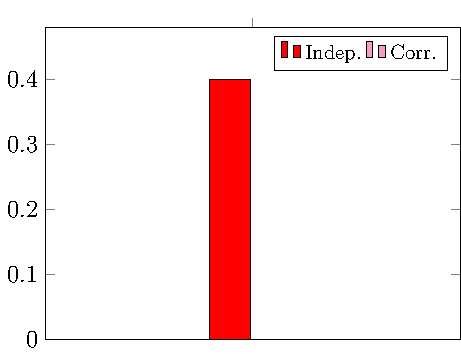
\includegraphics[width=\textwidth]{AppendixFigures/apx_marital-figure0.pdf}%{Figures/fig_score_col.pdf}%{Figures/shap_spearman_colinear.png}
    
    %               %\includegraphics[width=.9\linewidth]{Final_Figures/fig9b.png}%{Figures/shap_spearman_colinear.png}
    %               \caption{LIME}%Spearman rank correlations of signed feature importance magnitudes from SHAP and LIME against the true ranking from $\mathcal{G}$.}
    %                \label{apx_fig:marital_sign_accs_lime}
    %             \end{subfigure}
                
    %             \caption{Bar charts showing how SHAP and LIME (almost) never can correctly identify the sign of ``Married" when it is used to determine ``Cosigner."}%rankings of age and credit score change from when being independent to when credit score becomes a function of age}
    %             \label{apx_fig:marital_sign_accs}
    %         \end{figure}

    %         \begin{figure}[ht!]
    %             \centering
    %             \begin{subfigure}{.28\textwidth}
    %               \centering
    %               \captionsetup{justification=centering}
    %               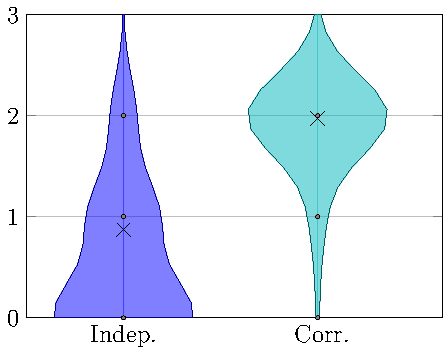
\includegraphics[width=\textwidth]{AppendixFigures/apx_marital-figure2.pdf}%{Figures/fig_age_col.pdf}%{Figures/lime_spearman_colinear.png}
    %                             %\includegraphics[width=.9\linewidth]{Figures/lime_shap_Spearman_magnitude.png}
    
    %               \caption{SHAP}%Spearman rank correlations of ranked feature importance magnitudes from LIME against the true ranked magnitudes from $\mathcal{G}$.}
    %                \label{apx_fig:marital_rank_diff_shap}
    %             \end{subfigure}%
    %             \hspace{3cm}
    %             \begin{subfigure}{.28\textwidth}
    %               \centering
    %                  \captionsetup{justification=centering}
    %               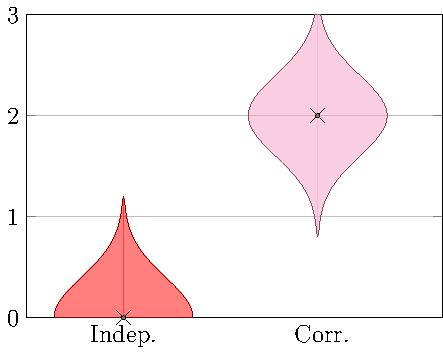
\includegraphics[width=\textwidth]{AppendixFigures/apx_marital-figure3.pdf}%{Figures/fig_score_col.pdf}%{Figures/shap_spearman_colinear.png}
    
    %               %\includegraphics[width=.9\linewidth]{Final_Figures/fig9b.png}%{Figures/shap_spearman_colinear.png}
    %               \caption{LIME}%Spearman rank correlations of signed feature importance magnitudes from SHAP and LIME against the true ranking from $\mathcal{G}$.}
    %                \label{apx_fig:marital_rank_diff_lime}
    %             \end{subfigure}
                
    %             \caption{Violin plots showing the differences between the given rank and true rank of ``Married" depending on whether ``Married" influences ``Cosigner." Lower is better.}%rankings of age and credit score change from when being independent to when credit score becomes a function of age}
    %             \label{apx_fig:marital_rank_diff}
    %         \end{figure}


    
    % % \subsubsection{Pervasiveness of Data-Misalignment}
    % %     Full details for the experimental design used in Section \ref{sec:pervasive} follow. We synthesize 100 datasets with randomly selected numbers of features between 3 and 100, and randomly selected numbers of rows between 100 and 10000. The features are i.i.d. according to $\mathcal{N}(0,5)$. The target of each dataset is binary and is produced using randomly generated linear decision boundaries. To generate the linear decision boundaries, we randomly generated integer coefficients between -10 and 10 which were then supplied to SymPy, which constructed the linear decision function which we then used to generate labels for each sample.  We vary the amount of label noise in each dataset by fixing a probability $p \in [0,.1]$ before generating the dataset and then flipping each label with probability $p$. We split each dataset into 80\% training data and 20\% testing data.

    % %     We generate a model for each dataset using the Python AutoML package auto-sklearn \citep{feurer-neurips15a}. We do not allow the AutoML to perform feature pre-processing. We set the AutoML to search among the following model types: NN, XGBoost, AdaBoost, Decision Tree, ExtraTrees, and Random Forest. We run the AutoML in a parellelized fashion with 16 cores and allow a maximum of 10 minutes to produce a model for each dataset. 

    % %     Since the number of features differs across the datasets, we report the results for our three metrics in the following fashion, conditioned on the number of features. For directionality, for each $d$, we report the mean directionality for the actual most important feature over 100 test set instances from the datasets with dimension $d$. Similarly, we report the feature-wise mean directionality and the percentage of features whose directionality was under $.5$. We also report the mean concordance and mean relevance for $k=3$ in the same fashion. We report the information similarly for the number of rows $n$ rather than $d$ below.

    % %   \begin{figure}[ht!]
    % %   \captionsetup{labelfont=footnotesize,textfont=footnotesize}
    % %   \captionsetup[subfloat]{labelfont=scriptsize,textfont=scriptsize,justification=centering}
    % %   \centering
    % %   \subfloat[SHAP Mean Directionality]{%
    % %     \hspace{0mm}
    % %     \raisebox{0cm}{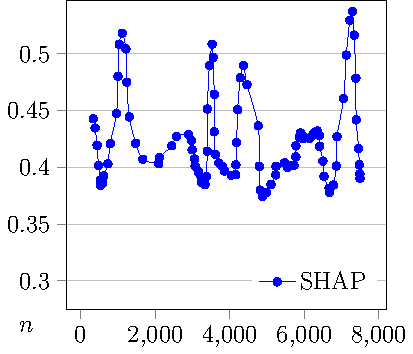
\includegraphics[width=0.178125\textwidth]{SynthFigs/meanaccshap_n-figure0.pdf}\quad}%
    % %     \label{apx_fig:shap_vary_n_spearmans}%
    % %   }\hspace{1cm}%\hfill
    % %   \subfloat[SHAP Concordance]{%
    % %     \raisebox{0cm}{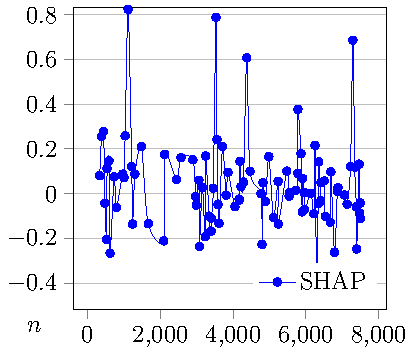
\includegraphics[width=0.178125\textwidth]{SynthFigs/concshap_n-figure0.pdf}}%
    % %     \label{apx_fig:shap_vary_n_accs}%
    % %   }\hspace{1cm}%\hfill
    % %   \subfloat[SHAP Top-3 Relevance]{%
    % %     \raisebox{0cm}{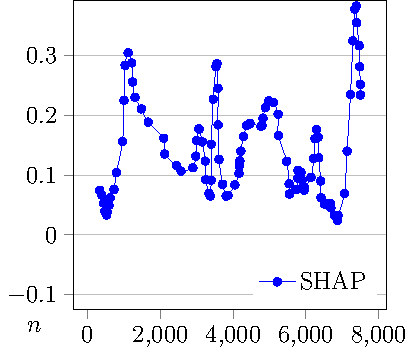
\includegraphics[width=0.178125\textwidth]{SynthFigs/relshap_n-figure0.pdf}}%
    % %     \label{apx_fig:shap_vary_n_spearmans}%
    % %   }\\
    % %   % \subfloat[LIME Top-1 Directionality]{%
    % %   %   \raisebox{0cm}{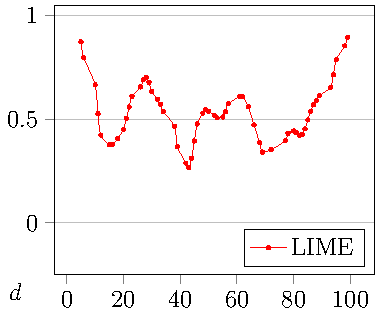
\includegraphics[width=.2\textwidth]{Figs/synthetic-figure1.pdf}}%
    % %   %   \label{fig:lime_vary_d_accs}%
    % %   % }\hspace{.5cm}%\hfill
    % %   \subfloat[LIME Mean Directionality]{%
    % %     \hspace{0mm}
    % %     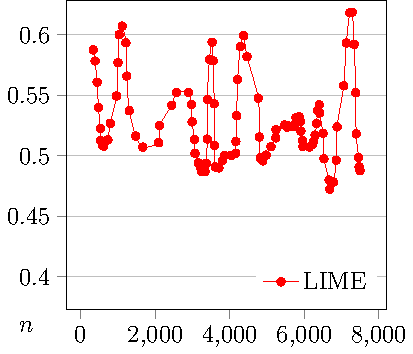
\includegraphics[width=0.178125\textwidth]{SynthFigs/meanacclime_n-figure0.pdf}\quad%
    % %     \label{apx_fig:lime_vary_n_spearmans}%
    % %   }\hspace{1cm}%\hfill
    % %   \subfloat[LIME Concordance]{%
    % %     \hspace{0mm}
    % %     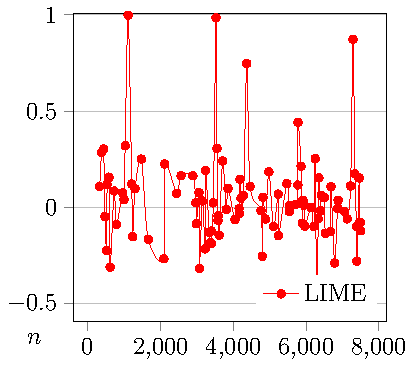
\includegraphics[width=0.178125\textwidth]{SynthFigs/conclime_n-figure0.pdf}%
    % %     \label{apx_fig:lime_vary_n_accs}%
    % %   }\hspace{1cm}%\hfill
    % %   \subfloat[LIME Top-3 Relevance]{%
    % %     \hspace{0mm}
    % %     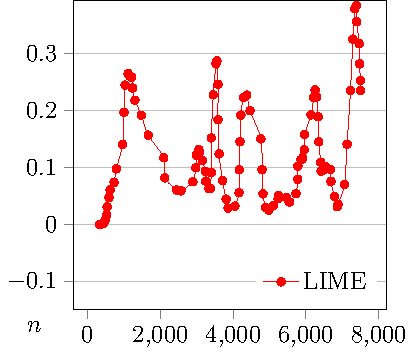
\includegraphics[width=0.178125\textwidth]{SynthFigs/rellime_n-figure0.pdf}%
    % %     \label{apx_fig:lime_vary_n_spearmans}%
    % %   }\\
    % %   \caption{Relationship of number of rows $n$ with feature-wise mean directionality, concordance, and relevance for $k=3$}
    % %   \label{apx_fig:lime_shap_vary_n}
    % % \end{figure}

    
    
   

    
    

    % % % \subsection{Details and  Experiments Related to Inconsistency}
    % % %     \label{apx_sec:inconsistency}
    % % %     In this section, we provide a more thorough analysis of the phenomenon of explainer inconsistency. We begin by discussing how the large number of unique mappings from $X$ to $Y$ in ML models' search spaces leads to an even larger number of potential explanations for phenomena regarding $X\rightarrow Y$. Then we investigate how, even if one fixes an ML model $\mathcal{M}$, there are many potential explanations for each prediction $\mathcal{M}(\boldsymbol{\xi})$ because of inconsistency between distinct explainer models and within the same explainer model. Finally, we demonstrate the problem of instability, where, fixing a model and explainer, explanations of the model's predictions on two similar inputs are very dissimilar. 
        
    % % %     \subsubsection{Prediction Stage Issues: Diversity of Decision Boundaries for $\mathcal{M}$}
    % % %         \label{sec:rashomon_overfitting}
    % % %         Because SHAP and LIME aim to approximate the local behavior of $\mathcal{M}$, their explanations are governed by $\mathcal{M}$'s decision boundary \citep{han22which}. This entails that explanations for the same prediction task differ across both model classes and across unique members of each model class. For example, explanations of decision trees and neural networks differ because decision trees partition the data space into rectangular regions while neural networks can partition the data space into irregularly shaped regions. Furthermore, two decision trees with different splits will partition the data into different rectangular regions. 
    
    % % %         % consider mentioning bootstrap
    % % %         Additionally, because models $\mathcal{M}$ are trained to achieve good predictive performance on given input data, the training data also affects explanations. Different pre-processing methodologies change the representation of the mapping from the features to the target that $\mathcal{M}$ aims to approximate, and therefore affects explanations by e.g. changing the meaning of feature importance. Also, measurement error and bias in the dataset limit how faithful $\mathcal{M}$ can be to the underlying true $\mathcal{G}$ and hence limit how much information about the marginal effects can be extracted. 
            
    % % %         %The inconsistency of explanations is, furthermore, related to the diversity of decision boundaries in two senses of the word diversity. First, different models necessarily have different decision boundaries. Second, the volatility of a decision boundary contributes to explanation instability.
    
    
    % % %         % put this first per dr. wang's request
    % % %         % talk about model performance and rashomon mayble?
    % % %         \paragraph{\textbf{Inconsistency from  Choices for $\mathcal{M}$}}
    % % %         Despite being trained on the same data and attaining approximately the same predictive performance, explanations of two distinct models with different decision boundaries will necessarily be different. Note that two unique decision boundaries could be obtained for the same dataset by the same class of models, e.g. by training two decision trees with differing maximum tree depths. Figure \ref{box} demonstrated how different explanations of two models from different classes can be by showing that SHAP's explanations for why the same applicant was approved by NN and XGBoost models were both misaligned and in different ways. Thus, different pipelines using different models tend to yield different explanations, none of which are necessarily representative of the actual marginal effects.
    
    % % %         % DOUBLE CHECK THE SHAP RESULT
    % % %         We illustrate the problem of inconsistency in greater generality by checking how often  feature importance signs and feature rankings of $m=100$ applicants agree when produced by combinations of the following models $\mathcal{M}$ and explainers $\mathcal{E}$. We consider three models with ROC AUC at least $.9$, an NN $\mathcal{M}_{\text{MLP}}$, and two distinct XGBoost models $\mathcal{M}_{\text{XGB1}}$ and $\mathcal{M}_{\text{XGB2}}$. We consider two explainers, $\mathcal{E}_{\text{LIME}}$ and $\mathcal{E}_{\text{SHAP}}$.
            
            
    % % %         We showcase inconsistency between models from different model classes by investigating the agreement between the explanations produced by $(\mathcal{M}_{\text{MLP}}, \mathcal{E}_{\text{LIME}})$ and $(\mathcal{M}_{\text{XGB1}}, \mathcal{E}_{\text{LIME}})$ as well as those between $(\mathcal{M}_{\text{MLP}}, \mathcal{E}_{\text{SHAP}})$ and $(\mathcal{M}_{\text{XGB1}}, \mathcal{E}_{\text{SHAP}})$. Figure \ref{fig:mlp_xgb_corr} shows that credit score was the only feature which consistently got the same feature importance sign. Also, on average, rankings from explanations of the NN and XGBoost were nearly uncorrelated for both SHAP and LIME. Since researchers should not, therefore, expect to get the same insights about marginal effects from explanations of models from two different model classes, the choice of what model to explain becomes an issue without a clear solution.
    % % %         % SHAP and LIME explanations of two pairs of models, all with AUC$\simeq .85$. The first pair consists of one NN and one XGBoost, while the second pair consists of two distinct XGBoost models. Figure \ref{fig:model_corrs} presents the results for both pairs. 
            
    % % %         Next, we showcase that there is also inconsistency between explanations of models from the same class by considering explanations between   $(\mathcal{M}_{\text{XGB1}}, \mathcal{E}_{\text{LIME}})$ and $(\mathcal{M}_{\text{XGB2}}, \mathcal{E}_{\text{LIME}})$ as well as those between $(\mathcal{M}_{\text{XGB1}}, \mathcal{E}_{\text{SHAP}})$ and $(\mathcal{M}_{\text{XGB2}}, \mathcal{E}_{\text{SHAP}})$, where XGB1 and XGB2 are XGBoost models which are made distinct by changing the random seed used for initialization in their otherwise identical training routine. Figure \ref{fig:xgb_xgb_corr} shows that SHAP had perfect agreement in all explanations while LIME was very inconsistent. SHAP's feature importance signs were completely consistent, while LIME's were only consistent for credit score. The mean concordance for SHAP is about 1 and the mean correlation for LIME is low, just above .25. The reason SHAP's explanations are perfectly consistent is because, when explaining the XGBoost models, all features except for credit score and income are always given Shapley values of 0. 
    % % %         The results from Figures \ref{fig:mlp_xgb_incon} and \ref{fig:xgb_xgb_incon} therefore suggest that there is usually disagreement in the feature rankings obtained by explaining two different models, but perhaps not when SHAP is explaining two models of the same type. 
            
    % % %         % \begin{figure}[ht!]
    % % %         % \centering
    % % %         %     \begin{subfigure}[t]{0.28\textwidth}
    % % %         %     \centering
    % % %         %     \captionsetup{width=1.6\linewidth}
    % % %         %     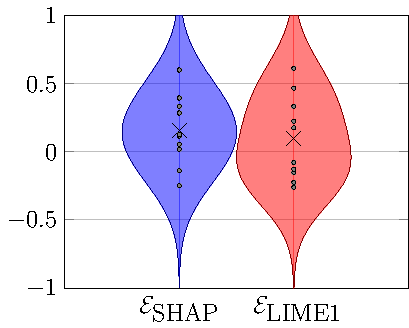
\includegraphics[width=\textwidth]{Figs/sec5_2_incon-figure0.pdf}
    % % %         %     \caption{Correlation between pairs of explanations of an NN and XGBoost model} \label{fig:mlp_xgb_corr}
    % % %         % \end{subfigure}
    % % %         % \hspace{2cm}
    % % %         % \begin{subfigure}[t]{0.28\textwidth}
    % % %         %     \centering
    % % %         %     \captionsetup{width=1.6\linewidth}
    % % %         %     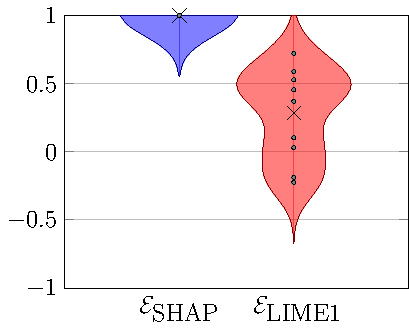
\includegraphics[width=\textwidth]{Figs/sec5_2_incon-figure1.pdf}
    % % %         %     \caption{Correlation between pairs of explanations from two distinct XGBoost models} 
    % % %         %     \label{fig:xgb_xgb_corr}
    % % %         % \end{subfigure}
    % % %         % \caption{Violin plots of Spearman correlations between pairs of explanations of different combinations of black box models}
    % % %         % \label{fig:model_corrs}
    % % %         % \end{figure}
    
    % % %         \begin{figure}[ht!]
    % % %         \centering
    % % %         \begin{subfigure}[t]{0.28\textwidth}
    % % %             \centering
    % % %             %\captionsetup{width=1.6\linewidth}
    % % %             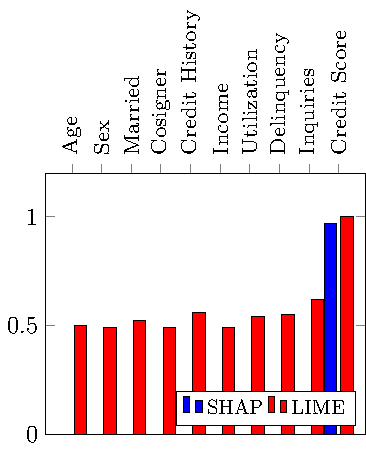
\includegraphics[width=\textwidth]{Figs/sec5_2_incon-figure4.pdf}
    % % %             \caption{Sign Agreement} 
    % % %             \label{fig:mlp_xgb_sgn}
    % % %         \end{subfigure}
    % % %         \hspace{2cm}
    % % %             \begin{subfigure}[t]{0.28\textwidth}
    % % %             \centering
    % % %             %\captionsetup{width=1.6\linewidth}
    % % %             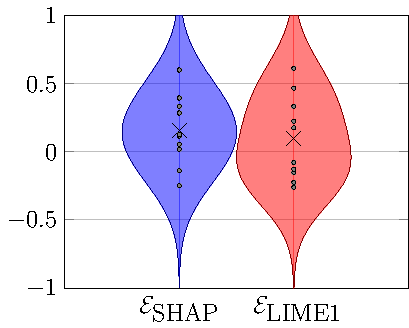
\includegraphics[width=\textwidth]{Figs/sec5_2_incon-figure0.pdf}
    % % %             \caption{Correlation} \label{fig:mlp_xgb_corr}
    % % %         \end{subfigure}
    % % %         \caption{Agreement between pairs of explanations of an NN and XGBoost model}
    % % %         \label{fig:mlp_xgb_incon}
    % % %         \end{figure}
    
    % % %         \begin{figure}[ht!]
    % % %         \centering
    % % %         \begin{subfigure}[t]{0.28\textwidth}
    % % %             \centering
    % % %             %\captionsetup{width=1.6\linewidth}
    % % %             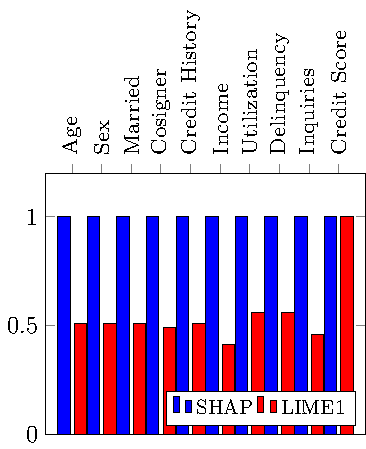
\includegraphics[width=\textwidth]{Figs/sec5_2_incon-figure6.pdf}
    % % %             \caption{Sign Agreement} 
    % % %             \label{fig:xgb_xgb_sgn}
    % % %         \end{subfigure}
    % % %             \begin{subfigure}[t]{0.28\textwidth}
    % % %             \centering
    % % %             %\captionsetup{width=1.6\linewidth}
    % % %             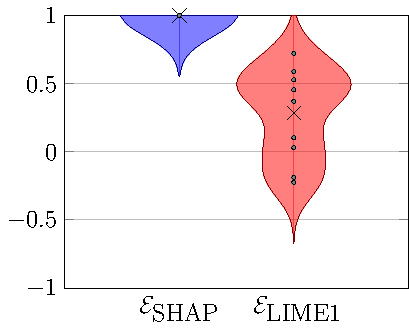
\includegraphics[width=\textwidth]{Figs/sec5_2_incon-figure1.pdf}
    % % %             \caption{Correlation} \label{fig:xgb_xgb_corr}
    % % %         \end{subfigure}
    % % %         \caption{Agreement between pairs of explanations from two distinct XGBoost models}
    % % %         \label{fig:xgb_xgb_incon}
    % % %         \end{figure}
    
    
    % % %         % instability moved to appendix
    % % %         %
            
    % % %         % \paragraph{\textbf{Inconsistency from Data pre-processing Methodology}}
    % % %         %     We identify two ways data pre-processing can affect post hoc explanations. First, the pre-processing affects the decision boundaries of models trained on it, which we know from Section \ref{sec:causes_of_misalignment} affects explanations. Second, pre-processing routines like standardization can change the signs of feature values, which we know from Section \ref{sec:theoretical_considerations} can cause the Shapley value sign to differ from that of $\boldsymbol{\beta}$. 
    
    % % %         %     To test this, we constructed two models $\mathcal{M}$ and $\mathcal{M}_{\text{Std.}}$ that were trained on the same dataset without and with feature standardization, respectively. $\mathcal{M}_{\text{Std.}}$ has associated pairs of explainers $\mathcal{E}_{\text{LIME Std.}}$ and $\mathcal{E}_{\text{SHAP Std.}}$. Similarly, $\mathcal{M}$ has associated pairs of explainers $\mathcal{E}_{\text{LIME}}$ and $\mathcal{E}_{\text{SHAP}}$.
                
                
    % % %         %     We then compared $(\mathcal{M}_{\text{Std.}}, \mathcal{E}_{\text{LIME Std.}})$ and $(\mathcal{M}_{\text{Std.}}, \mathcal{E}_{\text{SHAP Std.}})$ with explanations from pipelines pipelines $(\mathcal{M}, \mathcal{E}_{\text{LIME}})$ and $(\mathcal{M}, \mathcal{E}_{\text{SHAP}})$, respectively. It is evident from our results, shown in Figure \ref{fig:lime_shap_preproc_corr}, that neither SHAP nor LIME were robust to data normalization. SHAP's relatively worse sensitivity to data standardization can be explained by Equation \ref{eqn:shap_gt}, since the SHAP value of a feature depends linearly on both the value and mean of that feature. 
        
    % % %         %     \begin{figure}[ht!]
    % % %         %         \centering
    % % %         %         %\begin{subfigure}{.3\textwidth}
    % % %         %           \centering
    % % %         %           \captionsetup{justification=centering}
    % % %         %           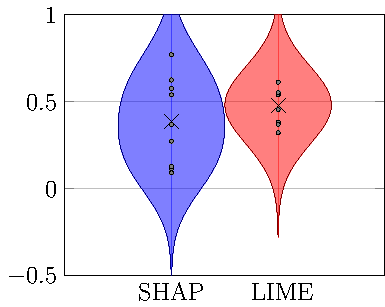
\includegraphics[width=.28\textwidth]{Figs/apx_preproc-figure3.pdf}
    % % %         %           \caption{Correlations between feature rankings from explanation of model trained on standardized data with feature rankings from explanations of model trained on data with no standardization}%Spearman rank correlations of ranked feature importance magnitudes from LIME against the true ranked magnitudes from $\mathcal{G}$.}
    % % %         %            %\label{fig:lime_income}
    % % %         %         %\end{subfigure}%
    % % %         %         %\caption{}%Violin plots of feature importance values for \emph{income} from SHAP and LIME for cases when \emph{income} is unconfounded and confounded by the unobserved social support feature}
    % % %         %         \label{fig:lime_shap_preproc_corr}
    % % %         %     \end{figure}
    
        
        
    
    
        
        
    % % %     \subsubsection{Explanation Stage Issues: Inconsistency Between and Within Explainers}
    % % %         \label{sec:conflict_between_within}
    % % %             %To motivate the use of multiple post hoc explainers, we show that they may explain the same outcome in different ways with differing degrees of accuracy. 
    % % %             Inconsistency also comes from the explanation stage since
    % % %             different explanations can be obtained by different explainers, or the same explainer method with different hyperparameters.
    % % %             We will demonstrate this by showing that not only do SHAP and LIME disagree in their explanations, but two distinct LIME explainers can also disagree. In view of Theorems 1 and 2, unmodified explanations from SHAP and LIME should not agree, so we compare LIME explanations with normalized SHAP explanations. 
                
    % % %             % move to discussion
    % % %             %\citep{visani21stability}, for example, studied the theoretical side of the issue by showing that LIME explanations are statistically not repeatable under identical conditions of explanation generation. \citep{kommiya21towards} showed that feature rankings from LIME, SHAP, and counterfactual explainers are often uncorrelated (especially with large data dimensions). \citep{Krishna2022TheDP} studied the practical side of the issue and showed (from interviews) that practitioners given multiple explanations from multiple explainers are forced to make confusing and somewhat arbitrary choices of what explanation to keep.
    % % %                 To test how consistent SHAP and LIME are with each other, we use both explainers to explain the same set of predictions by the same machine learning model XGB1 which we defined in the previous section and compare the results. For each of the $i=1,\ldots,m$ instances $\mathbf{x}^{(i)}$ we compute the sign agreement and rank correlation between the pair of explanations $e_\text{SHAP}(\mathbf{x}^{(i)})$ and $e_\text{LIME}(\mathbf{x}^{(i)})$. The results of our experiment, illustrated in Figure \ref{fig:lime_shap_incon}, show that the SHAP and LIME explanations of XGB1 are not consistent with each other. There is no substantial agreement in feature importance sign for any feature except or credit score (recall that SHAP assigns all features but credit score and income 0 importance when explaining XGB1). Unsurprisingly, the mean rank correlation between the pairs of explanations is close to 0, indicating that SHAP and LIME generally disagree in their rankings. It is worth noting that the level of disagreement would be \emph{worse} if we did not normalize the SHAP values. 
                    
                
                    
    % % % % new experiment
    % % % % signs feature importance values
    % % % % Fig 1 a: pick one instance, run LIME 10 times with different seeds, and show a bar plot for the percentages of positive values and negative values for the most important feature. （pick a good example - percentages are very different, 90% vs 10% -- low entropy)
    % % % % Fig 1 b: pick one instance, run LIME 10 times with different seeds, and show a bar plot for the percentages of positive values and negative values for the most important feature. (pick a bad example - percentages are very similar, 50% vs 50% -- high entropy)
    % % % % Fig 1 c: for the above experiment, compute the entropy of that two percentages (smaller the better), repeat the experiment on 100 instances and plot a violinplot
    % % % % ranking of feature importance
    % % % % Fig 2 a & b: pick one instance, run LIME 10 times with different seeds, show the distribution (histogram) of ranking for two features.
    % % % % Fig 2 c: for a given instance, run LIME 10 times with different seeds, each time getting a ranking of feature importance. Out of the total 10 rankings, do a pairwise comparison, which produces 45 pairs of Spearman rank correlation. Repeat on 100 instances. violinplot the 45 * 100 Spearman rank correlation.
    
    
    
    % % %     %        
    % % % In addition to different types of explainers disagreeing with each other, it is unfortunately also the case that individual explainers of the same type can produce a set of explanations for the same input that has some internal disagreement. We demonstrate this phenomenon with LIME only because SHAP is deterministic. %%The points generated in the sampling step are determined by random seed, the number of samples to generate around the point to explain, the kernel function (default Gaussian), and the kernel width defining the size of the neighborhood around the point to explain. 
    % % %             % i used signed feature importance vals here
    % % %            We constructed two unique LIME explainers $\mathcal{E}_{\text{LIME1}}$ and $\mathcal{E}_{\text{LIME2}}$ and computed the concordance between explanations from $(\mathcal{M}_{\text{XGB1}}, \mathcal{E}_{\text{LIME1}})$ and $(\mathcal{M}_{\text{XGB1}}, \mathcal{E}_{\text{LIME2}})$ and plotted the results in Figure \ref{fig:lime_corrs}. The first explainer had default hyperparameter settings and the second used a smaller kernel width. Since most of the violin area in Figure \ref{fig:lime_lime_xgb_corr} is below 1, this means that the two LIME explainers disagreed on almost every explanation. The nature of the disagreement was such that the pairs of explanations consistently assigned different signs to all features except for cosigner. Researchers may reasonably anticipate that repeated uses LIME to explain the same prediction will give different results and make selecting which explanation(s) to use in their study challenging. 
    
      
    % % % % \begin{figure}[ht!]
    % % % % \centering
    % % % %     \begin{subfigure}[t]{0.28\textwidth}
    % % % %     \centering
    % % % %     \captionsetup{width=1.6\linewidth,justification=centering}
    % % % %     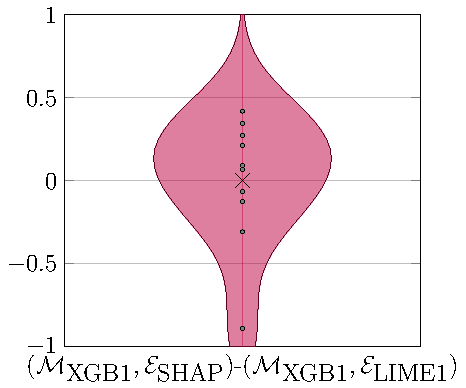
\includegraphics[width=\textwidth]{Figs/sec5_2_incon-figure2.pdf}
    % % % %     \caption{Correlation between SHAP and LIME explanations of pairs of explanations the same XGBoost model} \label{fig:lime_shap_xgb_corr}
    % % % % \end{subfigure}
    % % % % \hspace{2cm}
    % % % % \begin{subfigure}[t]{0.28\textwidth}
    % % % %     \centering
    % % % %     \captionsetup{width=1.6\linewidth,justification=centering}
    % % % %     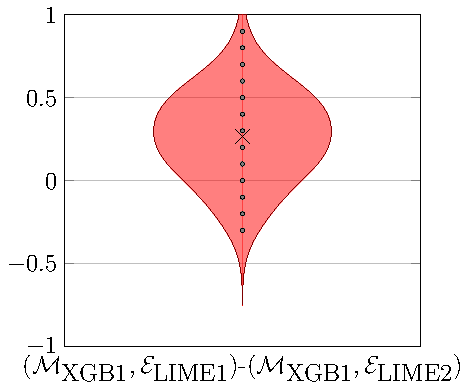
\includegraphics[width=\textwidth]{Figs/sec5_2_incon-figure3.pdf}
    % % % %     \caption{Correlation between pairs of explanations of the same XGBoost model from two distinct LIME explainers} \label{fig:lime_lime_xgb_corr}
    % % % % \end{subfigure}
    % % % % \caption{Violin plots of rank correlations between pairs of explanations of one XGBoost model from different combinations of explainers}
    % % % % \label{fig:explainer_corrs}
    % % % % \end{figure}
    % % % \begin{figure}[ht!]
    % % % \centering
    % % % \begin{subfigure}[t]{0.28\textwidth}
    % % %     \centering
    % % %     %\captionsetup{width=1.6\linewidth,justification=centering}
    % % %     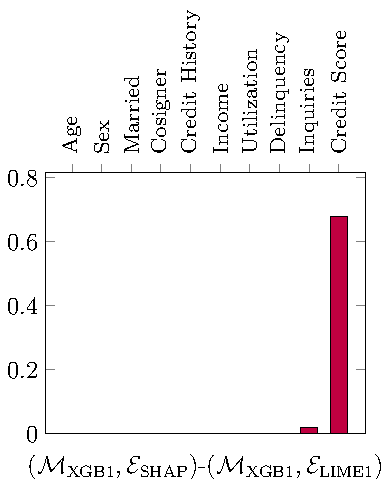
\includegraphics[width=\textwidth]{Figs/sec5_2_incon-figure7.pdf}
    % % %     \caption{Sign agreement}
    % % %     \label{fig:lime_shap_xgb_sgn}
    % % % \end{subfigure}
    % % % \hspace{2cm}
    % % %     \begin{subfigure}[t]{0.28\textwidth}
    % % %     \centering
    % % %     %\captionsetup{width=1.6\linewidth,justification=centering}
    % % %     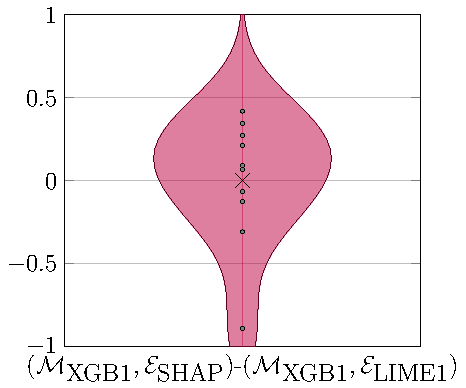
\includegraphics[width=\textwidth]{Figs/sec5_2_incon-figure2.pdf}
    % % %     \caption{Correlation} \label{fig:lime_shap_xgb_corr}
    % % % \end{subfigure}
    % % % \caption{Agreement between pairs of explanations of the same XGBoost model from SHAP and LIME}
    % % % \label{fig:lime_shap_incon}
    % % % \end{figure}
    
    % % % \begin{figure}[ht!]
    % % % \centering
    % % % \begin{subfigure}[t]{0.28\textwidth}
    % % %     \centering
    % % %     %\captionsetup{width=1.6\linewidth,justification=centering}
    % % %     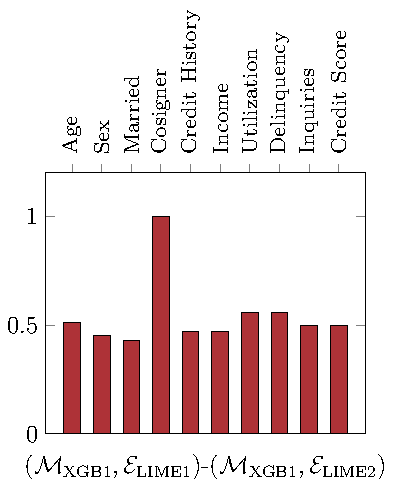
\includegraphics[width=\textwidth]{Figs/sec5_2_incon-figure8.pdf}
    % % %     \caption{Sign agreement} 
    % % %     \label{fig:lime_lime_xgb_sgn}
    % % % \end{subfigure}
    % % % \hspace{2cm}
    % % % \begin{subfigure}[t]{0.28\textwidth}
    % % %     \centering
    % % %     %\captionsetup{width=1.6\linewidth,justification=centering}
    % % %     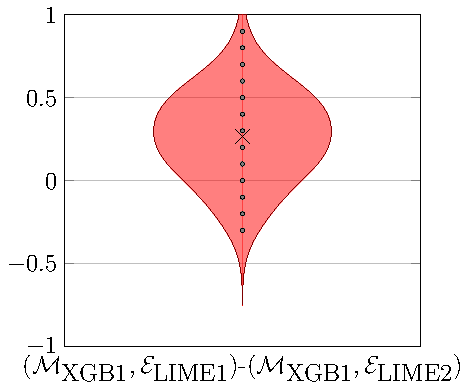
\includegraphics[width=\textwidth]{Figs/sec5_2_incon-figure3.pdf}
    % % %     \caption{Correlation } 
    % % %     \label{fig:lime_lime_xgb_corr}
    % % % \end{subfigure}
    % % % \caption{Agreement between pairs of explanations of the same XGBoost model from two distinct LIME explainers}
    % % % \label{fig:lime_corrs}
    % % % \end{figure}
        
    % % %     % % EXPOUND
         
         
    
    % % % %---------------------------------
    
    
            
    % % %         The second goal of this section is to introduce instability, another kind of inconsistency. 
            
        
    % % %     \subsubsection{Instability Due to Decision Boundary Volatility}         
    % % %         \label{sec:instability}
    % % %         Intuitively, explanations for the outcomes occurring in similar scenarios should be similar as well. In fact, the reasoning behind the decisions made on applicants with sufficiently similar profiles should be identical. Otherwise, applicants could have reason to suspect unfairness. But consider a situation where inputs $\boldsymbol{\xi}^{(1)}$ and $\boldsymbol{\xi}^{(2)}$ are nearby but $\mathcal{M}(\boldsymbol{\xi}^{(1)})$ and $\mathcal{M}(\boldsymbol{\xi}^{(2)})$ are distant. If one only cares about the faithfulness of the explainer with respect to $\mathcal{M}$, the explanations of $\boldsymbol{\xi}^{(1)}$ and $\boldsymbol{\xi}^{(2)}$ should definitely be dissimilar. However, if we care about faithfulness with respect to $\mathcal{G}$, and $\mathcal{G}(\boldsymbol{\xi}^{(1)})$ and $\mathcal{G}(\boldsymbol{\xi}^{(2)})$ are close, instability is not desirable. Instability is therefore a problem when an explainer is too unstable due to, e.g., overfitting. Both when $\mathcal{M}$ overfits $\mathcal{G}$ and when $\mathcal{E}$ overfits $\mathcal{M}$ can cause unnecessary variability to be captured by $\mathcal{E}$ and result in unnecessary instability. 
          
    % % %         To demonstrate instability, we construct a two-dimensional loan approval model based only on income and credit utilization and check the instability of LIME's coefficients when overfitting is and is not present. %Our approach for evaluating stability is similar to the coefficient stability index (CSI) from \citep{visani21stability}. 
    % % %         The first step of the experiment is to generate a dataset using a ground truth model $\mathcal{G}$ which decides approval using a linear combination of income and credit utilization. Then we train an NN $\mathcal{M}_1$ on a noisy version of that dataset where some points near the decision boundary of $\mathcal{G}$ have their label flipped. $\mathcal{M}_1$ misclassifies those noise points and is therefore meant to represent a classifier that did not overfit by fitting the noise points correctly. We construct another NN $\mathcal{M}_{2}$ which does overfit the noisy data and consequently has a comparatively erratic decision boundary. The decision boundaries of $\mathcal{M}_1$ and $\mathcal{M}_2$ are shown in Figure \ref{fig:dbds}. Finally, we quantify coefficient stability by computing the Euclidean distances between the LIME coefficients for pairs of LIME explanations of points near the decision boundary of $\mathcal{M}_1$ and their nearest neighbor with the same label. 

    % % %         Figure \ref{fig:dbd_dists} shows that explainers for $\mathcal{M}_{2}$ are more unstable than those for $\mathcal{M}_1$. This is evident because the distances between the coefficient sets of LIME explainers for pairs of nearby points are always much higher for LIME explainers of $\mathcal{M}_{2}$ than for explainers of $\mathcal{M}_1$.% When explaining $\mathcal{M}$, the mean distance is $9e-4$ and the standard deviation is $1e-3$, while when explaining $\mathcal{M}_{\text{overfit}}$, the mean distance is $2e-2$ and the standard deviation is $1.7e-2$. Explainers of $\mathcal{M}$ have high coefficient stability because the distances are concentrated near 0 in Figure \ref{fig:dbd_dists}. Explainers of $\mathcal{M}_{\text{overfit}}$ do not because the distance distribution is always much larger than 0. 

    % % %         \begin{figure}[ht!]
    % % %             \centering
    % % %             % \begin{subfigure}[t]{.3\textwidth}
    % % %             %   \centering
    % % %             %   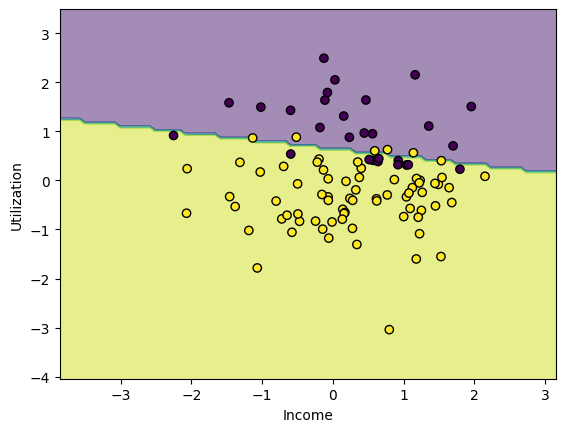
\includegraphics[width=\textwidth]{Figures/dbd_M.png}
    % % %             %   \caption{Decision boundary of $\mathcal{M}$}
    % % %             %   \label{fig:M_dbd}
    % % %             % \end{subfigure}%
    % % %             % \hfill
    % % %             % \begin{subfigure}[t]{.3\textwidth}
    % % %             %   \centering
    % % %             %   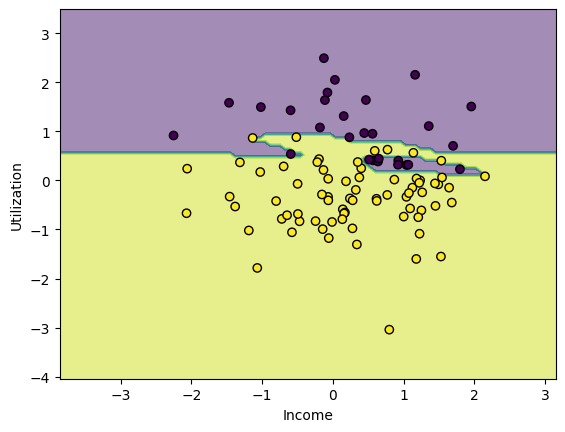
\includegraphics[width=\textwidth]{Figures/dbd_Mp.png}
    % % %             %   \caption{Decision Boundary of $\mathcal{M}_{\text{overfit}}$}
    % % %             %   \label{fig:Mp_dbd}
    % % %             % \end{subfigure}
    % % %             % \hfill
    % % %            \begin{subfigure}[t]{.28\textwidth}
    % % %             \centering
    % % %             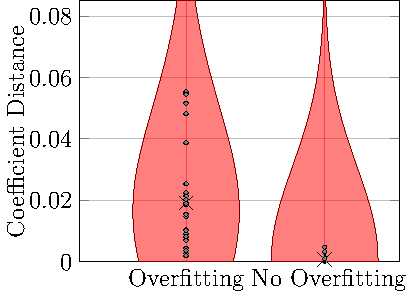
\includegraphics[width=\textwidth]{Figures/sec5_1_overfitting_spearmans.pdf}%{Figures/dbd_dists.png}
    % % %             %\caption{Effect of overfitting on stability}%Violin plots representing the stability of explainers of $\mathcal{M}$ and $\mathcal{M}_{\text{overfit}}$}
    % % %             \label{fig:dbd_dists}
    % % %             \end{subfigure}
    % % %             \caption{Violin plots representing the stability of explainers of $\mathcal{M}_1$ and $\mathcal{M}_2$. Each point represents the $L_2$ distance between the LIME coefficients for the explanation of a point near the decision boundary of $\mathcal{G}$ and its closest neighbor of the same class.}
    % % %             \label{fig:effect_of_overfitting}
    % % %         \end{figure}

    % % %         %\subsubsection{Decision Boundaries for Section on Decision Boundary Volatility}
    % % %         %    \label{sec:effect_of_overfitting}
    % % %             \begin{figure}[ht!]
    % % %                 \centering
    % % %                 \begin{subfigure}[t]{.28\textwidth}
    % % %                   \centering
    % % %                   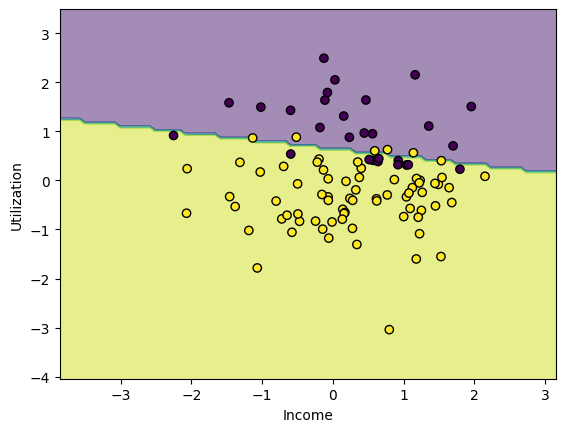
\includegraphics[width=\textwidth]{Figures/dbd_M.png}
    % % %                   \caption{Decision boundary of $\mathcal{M}$}
    % % %                   \label{fig:M_dbd}
    % % %                 \end{subfigure}%
    % % %                 \hspace{1cm}
    % % %                 \begin{subfigure}[t]{.28\textwidth}
    % % %                   \centering
    % % %                   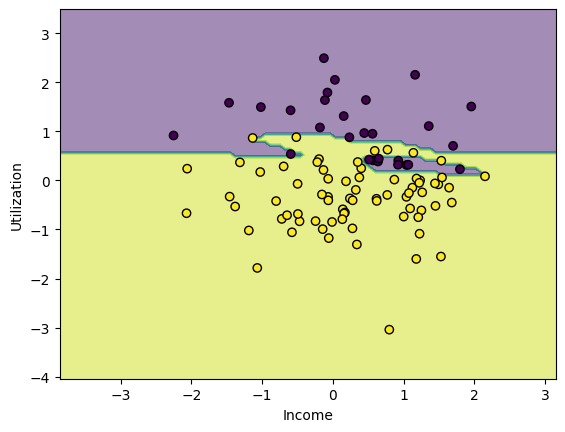
\includegraphics[width=\textwidth]{Figures/dbd_Mp.png}
    % % %                   \caption{Decision Boundary of $\mathcal{M}_{\text{overfit}}$}
    % % %                   \label{fig:Mp_dbd}
    % % %                 \end{subfigure}
    % % %                 \hspace{1cm}
    % % %                \begin{subfigure}[t]{.28\textwidth}
    % % %                 \centering
    % % %                 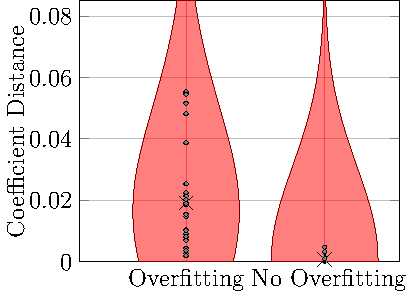
\includegraphics[width=\textwidth]{Figures/sec5_1_overfitting_spearmans.pdf}%{Figures/dbd_dists.png}
    % % %                 \caption{Effect of overfitting on stability}%Violin plots representing the stability of explainers of $\mathcal{M}$ and $\mathcal{M}_{\text{overfit}}$}
    % % %                 \label{fig:dbd_dists}
    % % %                 \end{subfigure}
    % % %                 \caption{Visualizations of decision boundaries for NNs that do and do not overfit ($\mathcal{M}$ and $\mathcal{M}_{\text{overfit}}$) on a simple two variable loan approval dataset. Yellow points are accepted applicants and purple points are denied applicants.}
    % % %                 \label{fig:dbds}
    % % %             \end{figure}
        
    % % %     \subsubsection{Effect of Data Pre-processing}
    % % %     We identify two ways data pre-processing can affect post hoc explanations. First, the pre-processing affects the decision boundaries of models trained on it, which we know from Appendix Section \ref{apx_sec:rashomon_overfitting} affects explanations. Second, pre-processing routines like standardization can change the signs of feature values, which we know from Section \ref{sec:theoretical_considerations} can cause the signs of a feature's Shapley value and marginal effect to differ.
    % % %         \begin{figure}[ht!]
    % % %             \centering
    % % %             %\begin{subfigure}{.28\textwidth}
    % % %               \centering
    % % %               \captionsetup{justification=centering}
    % % %               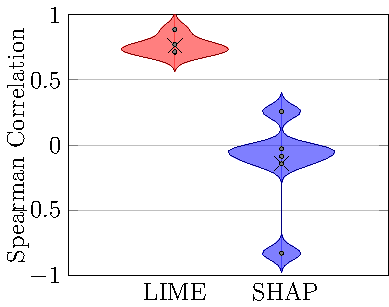
\includegraphics[width=.28\textwidth]{AppendixFigures/apx_preproc_rank_corrs.pdf}
    % % %               %\caption{Correlations between feature rankings from explanation of model trained on standardized data with feature rankings from explanations of model trained on data with no pre-processing}%Spearman rank correlations of ranked feature importance magnitudes from LIME against the true ranked magnitudes from $\mathcal{G}$.}
    % % %             %   \label{fig:lime_income}
    % % %             %\end{subfigure}%
    % % %             \caption{Correlations between feature rankings from explanation of model trained on standardized data with feature rankings from explanations of model trained on data with no pre-processing}%Violin plots of feature importance values for \emph{income} from SHAP and LIME for cases when \emph{income} is unconfounded and confounded by the unobserved social support feature}
    % % %             \label{fig:lime_shap_preproc_corr}
    % % %         \end{figure}
    
    
    
   

    
    
    
    
    
    
   
    
    
    \section*{Appendix B: Details on Mitigation Strategies}
        \label{apx_sec:mitigation_details}
        This section contains the details for the hypothesis testing framework we use to evaluate our mitigation strategies, as well as additional mitigation strategies. We motivate each test used and give the statements of the null and alternative hypotheses. Two more mitigation strategies involving ensembles of explainers are presented. 
        
        \subsubsection{Hypothesis Testing for Improvement}
            \label{apx_sec:hypothesis_testing}
            In this section, we will describe our hypothesis testing framework for improvement of data-alignment. We will abuse notation here and, for example, consider $\mE$ to be LIME with default settings explaining an NN $\mathcal{M}_1$ and $\mE^\prime$ to be an explanation method that applies some mitigation strategies we propose. Thus, the notation $\mE$ and $\mE^\prime$ suppresses the models and data being used.
            
            Wilcoxon signed-rank tests are non-parametric tests for differences of populations, and thus applicable in our setting. Given two sets of measurements $A=\{a_i\}_{i=1}^m$ and $B=\{b_i\}_{i=1}^m$, Wilcoxon signed-rank tests operate on the matched differences $a_i-b_i$. We can view explanations from $\mE$ and $\mE^\prime$ as a matched sample since, for each $i$, $e_{\mE}(\mathbf{x}^{(i)})$ and $e_{\mE^\prime}(\mathbf{x}^{(i)})$ differ only by the explanation method used. We will assume that the differences are symmetrically distributed so that the null hypotheses declare the location of the population mean of the differences $a_i - b_i$. All tests will be performed with a significance level of $\alpha=.05$.

            Our use of Wilcoxon signed-rank tests is not exactly the same for all three metrics, but follows the following general framework in each case.
            Given a metric $m$, the null hypothesis $H_{0,\delta}$ asserts that $\mE^\prime$ and $\mE$ are the same on average with respect to the metric $m$ along a dimension $\delta$. If $m$ is directionality, then $\delta$ ranges over the feature indices $j=1,\ldots,D$. If $m$ is concordance, the notion of $\delta$ is irrelevant. If $m$ is relevance, $\delta$ ranges over $k=1,\ldots,D-1$.
            \begin{equation*}
                H_{0,\delta}: \text{ The } m_\delta(e_\mE(\bx^{(i)},\boldsymbol{\beta})) - m_\delta(\bx^{(i)},\boldsymbol{\beta})) \text{ are symmetric about } \mu = 0
            \end{equation*}
            $H_{1,\delta}$ asserts that $\mE^\prime$ is significantly worse than $\mE$ along dimension $\delta$. 
            \begin{equation*}
                H_{1,\delta}: \text{ The } m_\delta(e_\mE(\bx^{(i)},\boldsymbol{\beta})) - m_\delta(\bx^{(i)},\boldsymbol{\beta})) \text{ are symmetric about } \mu > 0
            \end{equation*}
            If we reject $H_{0,\delta}$ in favor of $H_{1,\delta}$ at the $\alpha=.05$ level for at least one $\delta$, we come to the conclusion that $\mE^{\prime}$ did not improve over $\mE$ with respect to $m$. Otherwise, and if $H_{0,\delta}$ is rejected in favor or the following $H_{2,\delta}$ for at least one $\delta$, we conclude that $\mE^{\prime}$ constitutes an improvement over $\mE$ with respect to $m$.
            \begin{equation*}
                H_{2,\delta}: \text{ The }  m_\delta(e_\mE(\bx^{(i)},\boldsymbol{\beta})) - m_\delta(\bx^{(i)},\boldsymbol{\beta})) \text{ are symmetric about } \mu< 0
            \end{equation*}            
            
            When applying this framework to directionality, the differences are $s_j(e_\mE(x_j^{(i)},\beta_j)) - s_j(e_{\mE^\prime}(x_j^{(i)},\beta_j))$. When applying this framework to concordance, $\delta=1$, the differences are $\text{\text{concordance}}(e_\mE(\mathbf{x}^{(i)}),\boldsymbol{\beta}) - \text{\text{concordance}}(e_{\mE^\prime}(\mathbf{x}^{(i)}))$, and $H_{1,1}$ is unused. When applying the framework to relevance the differences are $\text{relevance}_k(r(e_\mE(\mathbf{x}^{(i)}), r(\boldsymbol{\beta})) - \text{relevance}_k(r(e_{\mE^\prime}(\mathbf{x}^{(i)}), r(\boldsymbol{\beta}))$.
            
            


            
            
   
            % \paragraph{Test for Equality of Directionality}        We have two conditions for $\mE^\prime$ to improve over $\mE$ with respect to directionality stating that 1) the directionality of $\mE^\prime$ cannot be significantly worse than the directionality of $\mE$ for any feature, and 2) the directionality of $\mE^\prime$ must be significantly better than the directionality of $\mE$ for at least one feature. We implement this using the following two Wilcoxon signed-rank tests for each feature. We consider, for each feature $j$, the null hypothesis
            % \begin{equation*}
            %     H_0: \text{ The } s_j(e_\mE(x_j^{(i)},\beta_j) - s_j(e_{\mE^\prime}(x_j^{(i)},\beta_j) \text{ are symmetric about } \mu = 0
            % \end{equation*}
            % Then, to test if the directionality of $\mE^\prime$ was significantly worse than those of $\mE$, we test the following one-sided alternative hypotheses for each $j$.
            % \begin{equation*}
            %     H_1: \text{ The } s_j(e_\mE(x_j^{(i)},\beta_j) - s_j(e_{\mE^\prime}(x_j^{(i)},\beta_j) \text{ are symmetric about } \mu > 0
            % \end{equation*}
            % If we reject $H_0$ in favor of $H_1$ at the $\alpha=.05$ level, we come to the conclusion that $\mE^{\prime}$ did not improve over $\mE$ with respect to directionality. Otherwise, we move on to test the other one-sided alternative hypothesis for each $j$.
            % \begin{equation*}
            %     H_2: \text{ The }  s_j(e_\mE(x_j^{(i)},\beta_j) - s_j(e_{\mE^\prime}(x_j^{(i)},\beta_j) \text{ are symmetric about } \mu < 0
            % \end{equation*}
            % If we reject $H_0$ in favor of $H_2$ for at least one $j$, we come to the conclusion that $\mE^{\prime}$ improved over $\mE$ with respect to directionality. Otherwise, we conclude that there was no significant change. 
            
            % % are the ranks independent?
            % % In pairs(x,y), x is a measurement for individual I and y is a measurement coming from an identical copy of I...
            % \paragraph{Test for Equality of Concordance}  
            % We say that $\mE^\prime$ improves over $\mE$ in terms of concordance based on the result of a Wilcoxon signed-rank test with the following null and alternative hypotheses.
            % \begin{align*}
            %     H_0: \text{ The } \text{\text{concordance}}(e_\mE(\mathbf{x}^{(i)}),\boldsymbol{\beta}) - \text{\text{concordance}}(e_{\mE^\prime}(\mathbf{x}^{(i)})) \text{ are symmetric about } \mu=0 \\
            %     H_1: \text{ The } \text{\text{concordance}}(e_\mE(\mathbf{x}^{(i)}),\boldsymbol{\beta}) - \text{\text{concordance}}(e_{\mE^\prime}(\mathbf{x}^{(i)})) \text{ are symmetric about } \mu<0     \end{align*}
            % That is, we must reject the null hypothesis that the concordance distributions of $\mE$ and $\mE^\prime$ have the same mean.        
            % % cannot find implementation of multivariate KS test
            % %Finally, we say that $E^\prime$ improve over $E$ in terms of relevance if a Kolmogorov-Smirnov (KS) test is significant at the $\alpha=.05$ level. The KS test is a non-parametric test for equality of (continuous) distributions. We use the multivariate extension  
            % % is this not ok because the distributions for each k are related?
            % \paragraph{Test for Equality of Relevance}         As with the directionality metric, have two conditions for $\mE^\prime$ to improve $\mE$ based on one sided Wilcoxon signed-rank tests. First, $\text{relevance}_k$ for $\mE^\prime$ cannot be significantly worse than the $\text{relevance}_k$ of $\mE$ for any $k$. Likewise, the $\text{relevance}_k$ of $E^\prime$ must be significantly better than the$\text{relevance}_k$ of $\mE$ for at least one $k$. We formulate the null and alternative hypotheses which formalize the notion of significant improvement for each $k$ as follows.
            % \begin{align*}
            % H_0: \text{ The } \text{relevance}_k(r(e_\mE(\mathbf{x}^{(i)}), r(\boldsymbol{\beta})) - \text{relevance}_k(r(e_{\mE^\prime}(\mathbf{x}^{(i)}), r(\boldsymbol{\beta})) \text{ are symmetric about } \mu=0 \\
            % H_1: \text{ The }\text{relevance}_k(r(e_\mE(\mathbf{x}^{(i)}), r(\boldsymbol{\beta})) - \text{relevance}_k(r(e_{\mE^\prime}(\mathbf{x}^{(i)}), r(\boldsymbol{\beta})) \text{ are symmetric about } \mu > 0 \\
            % H_2: \text{ The } \text{relevance}_k(r(e_\mE(\mathbf{x}^{(i)}), r(\boldsymbol{\beta})) - \text{relevance}_k(r(e_{\mE^\prime}(\mathbf{x}^{(i)}), r(\boldsymbol{\beta})) \text{ are symmetric about } \mu<0      \end{align*}

%             \paragraph{Tests for Equality of Consistency}
%         We are interested in how consistent a method's feature importance values are across different factors of the pipeline when explaining a linear model since, ideally, they would always be data-aligned. Having established in Section \ref{sec:inconsistency} that different pairs of pipeline configurations often produce pairs of explanations such that the corresponding pairs of feature importance signs and rankings disagree, we will test for improvement of consistency in those two respects. To test whether a strategy improves consistency, we will compare a baseline pair of pipelines $\mE_1$ and $\mathcal{E}_2$ with a second pair of pipelines  $\mE^\prime_1$ and $\mE^\prime_2$ that employ the strategy we propose will improve consistency.

%         We characterize improvement of consistency of feature importance signs by requiring that the feature importance signs from $\mE^\prime_1$ and $\mE^\prime_2$ are more consistent than those from $\mE_1$ and $\mE_2$ for at least one feature and not less consistent for any features. To test for this, for each of the $j=1,\ldots,d$ features, we utilize a one-sided McNemar test with the following contingency table, and null and alternative hypotheses involving matched samples of feature importance signs. Using the sign function ($\text{sgn}(0)=0$ and $\text{sgn}(x)=\frac{x}{\mid x\mid})$ otherwise), we define the following contingency table.
% \begin{table}[ht]
% \centering
% \begin{tabular}{|l|l|l|}
% \hline
% & $\text{sgn}(e_{\mE^\prime_1}(x_j^{(i)}))=\text{sgn}(e_{\mE^\prime_2}(x_j^{(i)}))$ & $\text{sgn}(e_{\mE^\prime_1}(x_j^{(i)}))\neq\text{sgn}(e_{\mE^\prime_2}(x_j^{(i)}))$ \\ \hline
% $\text{sgn}(e_{\mE_1}(x_j^{(i)}))=\text{sgn}(e_{\mE_2}(x_j^{(i)}))$                  & a                                                                             & b                                                                                \\ \hline
% $\text{sgn}(e_{\mE^\prime_1}(x_j^{(i)}))\neq\text{sgn}(e_{\mE^\prime_2}(x_j^{(i)}))$ & c                                                                             & d                                                                                \\ \hline
% \end{tabular}
% \caption{Contingency table used for McNemar's test of marginal equivalences applied to testing for improvement to the consistency of the feature importance sign given to feature $j$.}
% \label{tab:my-table}
% \end{table}
% We define theoretical probabilities $p_a,p_b,p_c,p_d$ of occurrence in the cells $a,b,c,d$ such that $p_b$ and $p_c$ represent the probability that $\mE^\prime_1$ and $\mE^\prime_2$ give the same sign to a sample and the probability that $\mE_1$ and $\mE_2$ give the same sign to a sample, respectively. The null hypothesis asserts the equality of $p_b$ and $p_c$ and the alternative asserts that $p_b>p_c$, i.e. that the modified pipeline assigns feature importance signs more consistently.
%         \begin{align*}
%             & H_0: p_b = p_c \text{ (disagreement between $\mE_1$ and $\mE_2$ and disagreement between $\mE^\prime_1$ and $\mE^\prime_2$ is equally likely)}\\
%             & H_1: p_b > p_c \text{ ($\mE_1$ and $\mE_2$ are more likely to disagree)} 
%         \end{align*}
%         Thus, improvement occurs if $H_0$ is rejected in favor of $H_1$ for at least one feature and $H_0$ is not rejected in favor of $H_2$ for any feature.

        
%          We test for consistency of rankings as follows. Using the baseline pair of pipelines, we compute $C = \{\text{concordance}(e_{\mE_1}(\mathbf{x}^{(i)}), e_{\mE_2}(\mathbf{x}^{(i)}))\}_{i=1}^m$. Then, using the pair of pipelines involving the mitigation strategy of interest, we compute $C^\prime = \{\text{concordance}(e_{\mE^\prime_1}(\mathbf{x}^{(i)}), e_{\mE^\prime_2}(\mathbf{x}^{(i)}))\}_{i=1}^m$. We then perform a Wilcoxon signed-rank test with the following null and alternative hypotheses using $C$ and $C^\prime$ as matched samples. 
%         \begin{align*}
%             H_0: \text{ The } \text{concordance}(e_{\mE_1}(\mathbf{x}^{(i)}), e_{\mE_2}(\mathbf{x}^{(i)})) - \text{concordance}(e_{\mE^\prime_1}(\mathbf{x}^{(i)}), e_{\mE^\prime_2}(\mathbf{x}^{(i)})) \text{ are symmetric about } \mu=0 \\
%             H_a: \text{ The } \text{concordance}(e_{\mE_1}(\mathbf{x}^{(i)}), e_{\mE_2}(\mathbf{x}^{(i)})) - \text{concordance}(e_{\mE^\prime_1}(\mathbf{x}^{(i)}), e_{\mE^\prime_2}(\mathbf{x}^{(i)})) \text{ are symmetric about } \mu > 0   
%         \end{align*}
        
%         % are disjoint sets of applicants so that $C$ and $C^\prime$ can be taken to be independent. 
%         % Finally, we perform the following one-sided $F$-test for two variances at the $\alpha=.05$ significance level.

%         % \begin{align*}
%         %     H_0:\ \sigma_C^2 = \sigma_{C^\prime}^2 \\
%         %     H_a:\ \sigma_C^2 < \sigma_{C^\prime}^2 \\
%         % \end{align*}
        
       
        % \subsubsection{SHAP Value Normalization}
        %     \label{apx_sec:shap_norm_indep}

        %         Figure \ref{apx_fig:dividex} shows a comparison of the results we obtained by comparing default SHAP explanations with SHAP explanations modified by normalizing by $(\mathbf{x}-\bar{\mathbf{x}})$ and using the variant of our dataset with mutually independent features. It shows that by normalizing the Shapley value, SHAP sees significant increases in directionality for all features, movement of the mean concordance from 0 to near 1, and noteworthy increases to $\text{relevance}_k$ for $k=2,\ldots,5$. Indeed, normalizing the Shapley value yields a significant improvement for each of our three metrics. This result suggests that normalizing the Shapley value is necessary to obtain data-aligned explanations using SHAP.
        %             \begin{figure}[ht!]
        %         \centering
        %         \begin{subfigure}[t]{.28\textwidth}
        %           \centering
        %           \captionsetup{justification=centering}
        %               \raisebox{.2cm}{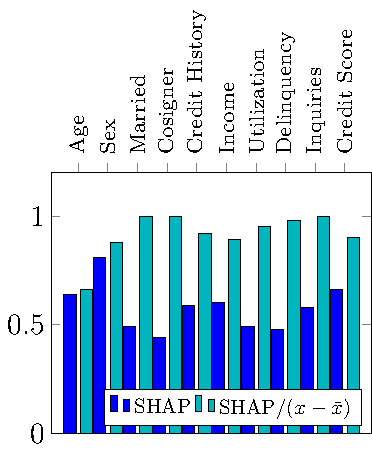
\includegraphics[width=\textwidth]{Figs/apx_dividex-figure0.pdf}}%{Figures/lime_shap_Spearman_magnitude.png}
    
        %           \caption{SHAP Directionality}%Spearman rank correlations of feature importance magnitudes from SHAP and LIME against the true ranking from $\mathcal{G}$. }
        %            \label{apx_fig:dividex_sign_accs}
        %         \end{subfigure}%
        %         \hspace{1cm}
        %         \begin{subfigure}[t]{.28\textwidth}
        %           \centering
        %            \captionsetup{justification=centering}
        %           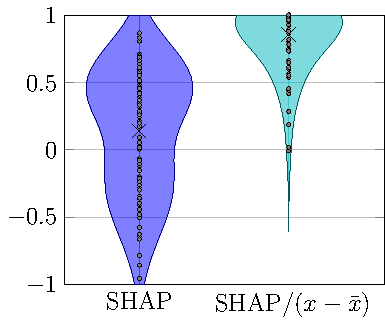
\includegraphics[width=\textwidth]{Figs/apx_dividex-figure1.pdf}%{Figures/lime_shap_Spearman_signed.png}
        %           \caption{SHAP Concordance}%Spearman rank correlations of signed feature importance from SHAP and LIME against the true ranking from $\mathcal{G}$.}
        %            \label{apx_fig:dividex_spearmans}
        %         \end{subfigure}
        %         \hspace{1cm}
        %         \begin{subfigure}[t]{.28\textwidth}
        %           \centering
        %            \captionsetup{justification=centering}
        %         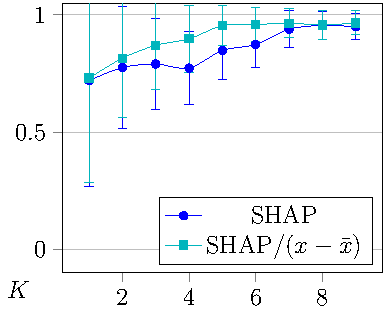
\includegraphics[width=\textwidth]{Figs/apx_dividex-figure2.pdf}%
        %         \caption{SHAP Relevance}%The average and standard error of recall of SHAP and LIME when attempting to capture the top K most important features to $\mathcal{G}$ when explaining $\mathcal{M}$, for varied $K=1,2,3,...$ number of features.}
        %         \label{apx_fig:dividex_recalls}
        %         \end{subfigure}
        %         \caption{Comparison of default and normalized SHAP explanations with respect to directionality, concordance, and relevance.}
        %        \label{apx_fig:dividex}
        %     \end{figure} 

    
    
    
  
    \subsection{Additional Mitigation Strategies}
        \label{apx_sec:additional_mitigations}
        In this section, we provide the results for mitigations strategies that we tried that are less effective or less intuitive/natural than those in the main paper. In particular, we explore two additional ways to use ensembles of explanations. They are both ways to aggregate explanations of a single model. 
        
        We propose that the primary reason these strategies did not work well is that the SHAP and LIME explanations do not satisfy the necessary criteria for the success of ensemble algorithms. Viewed as means for predicting the ranking of features with respect to their marginal effects, SHAP and LIME are neither weak nor strong classifiers. So, even though the simplicity of our aggregation techniques plays a role in the quality of our results, even if we were to develop a more sophisticated boost, bagging, or stacking method, the SHAP and LIME explanations would not satisfy the requirements necessary for those algorithms to work. %, then explore ways to select LIME explainers on the basis of their local predictive performance. 

            \subsubsection{Averaging SHAP and LIME Explanations}
            A simple way to resolve the difficulty in choosing whether to use SHAP or LIME is to use both and combine their results. Since SHAP and LIME have differing meanings of feature importance it does not make sense to aggregate them without further processing. We take two steps to address this. First, we normalize the Shapley values (following Section \ref{sec:theoretical_considerations}) so that both SHAP and LIME can be seen as approximating the marginal effects $\boldsymbol{\beta}$. Then we max-normalized the SHAP and LIME values so that they occur on the same scale. 

            Figure \ref{apx_fig:limeshap} displays a comparison between LIME, SHAP, and their average with respect to data-alignment. Figure \ref{apx_fig:limeshap_sign_accs} shows that, generally, at least one of LIME or SHAP has higher (or equal) directionality than their average for each feature. Figure \ref{apx_fig:limeshap_spearmans} shows that the mean concordances for LIME, SHAP, and their average are nearly equal. Figure \ref{apx_fig:limeshap_recalls} shows that relevance for the average is better than SHAP generally, better than LIME for $k=1$, and otherwise equal. Thus, this averaging scheme is evidently not significantly effective for increasing data-alignment. 

            

            \begin{figure}[!h]
            \centering
                \begin{subfigure}[t]{0.28\textwidth}
                \centering
                \raisebox{.2cm}{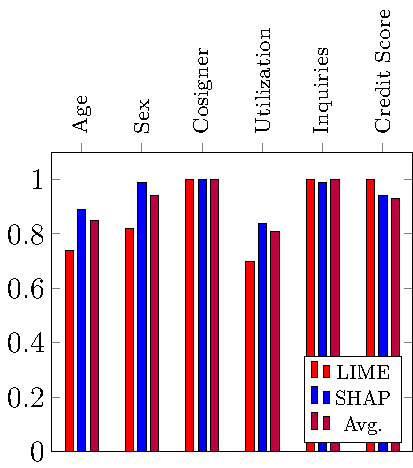
\includegraphics[width=\textwidth]{AppendixFigures/apx_limeshap-figure0.pdf}}
                \caption{Directionality} \label{apx_fig:limeshap_sign_accs}
            \end{subfigure}\hspace{1cm}
            \begin{subfigure}[t]{0.28\textwidth}
                \centering
                \raisebox{.05cm}{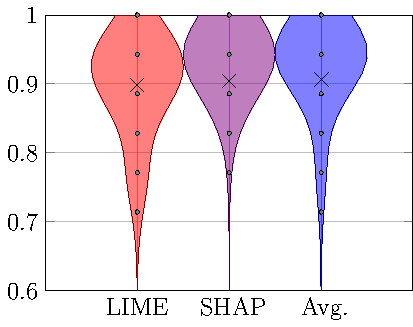
\includegraphics[width=\textwidth]{AppendixFigures/apx_limeshap-figure1.pdf}}
                \caption{Concordance} \label{apx_fig:limeshap_spearmans}
            \end{subfigure}\hspace{1cm}
             \begin{subfigure}[t]{0.28\textwidth}
                \centering
                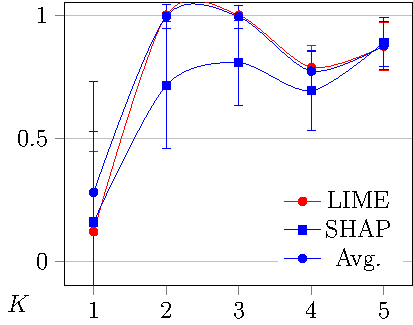
\includegraphics[width=\textwidth]{AppendixFigures/apx_limeshap-figure2.pdf}
                \caption{Relevance}
                \label{apx_fig:limeshap_recalls}
            \end{subfigure}
            \caption{Comparison of individual LIME and (normalized) SHAP explanations with explanations constructed by averaging the feature importance values between the two for each applicant}\label{apx_fig:limeshap}
            \end{figure}            

    % add this back if results are ok
    %     \subsubsection{Ensuring that LIME's Local Prediction is Correct} 
    %         \label{apx_sec:e_fidelity}
    %         Since the underlying linear model of a LIME explanation is constructed to be a good representative of $\mathcal{M}$'s local behavior, we hypothesized that the ability of a LIME explainer to correctly classify the label of the input being explained is related to the quality of the explanation for that input. Given an outcome $\mathcal{M}(\boldsymbol{\xi}) = y$ to be explained, the LIME package provides prediction probabilities for each possible label for $\boldsymbol{\xi}$. We will take $\hat{y}_{\text{LIME}}$ to be the label of the larger probability and attempt to clarify the relation between the condition $y = \hat{y}_{\text{LIME}}$ and the quality of LIME's explanations.
        
    %         We only consider LIME here because LIME's surrogate model is a linear approximation of $\mathcal{M}$ and SHAP's is not; the idea of predictive accuracy makes sense for LIME and not SHAP. Indeed, the concept of local fidelity is only relevant for explainers using surrogate models. Counterfactual explanations, for example, do not have a notion of local fidelity. 
            
    %         %The local fidelity of an explainer's surrogate model is the surrogate model's prediction accuracy with respect to $\mathcal{M}$ in a neighborhood of the point being explained \citep{laugel18defining}. 
    %         %We will define fidIntuitively, high local fidelity should be associated with faithful explanations. This section investigates this claim. We use LIME alone in our experiments because LIME's surrogate model is a linear approximation of $\mathcal{M}$ and SHAP's is not; the idea of local fidelity in terms of function approximation only makes sense for LIME. The concept of local fidelity is only relevant for explainers using surrogate models. Counterfactual explainers, for example, have no notion of local fidelity. For our experiment, we create a set of LIME explainers of varying degrees of local fidelity and record the quality of their explanations. 
        
    %         For our experiment, we create a set of LIME explainers with different hyperparameters and, for 100 applicants, record whether they correctly classify the applicants' loan decision and the quality of their explanations for those applicants. We have LIME explain an NN with AUC=.8 because if the AUC of $\mathcal{M}$ is very high, we observed that LIME surrogate models (almost) always correctly classify all loan decisions. For each applicant, we construct 100 LIME explainers using combinations of kernel widths $\nu$ in $\{.1\sqrt{d},.2\sqrt{d},\ldots,\sqrt{d}\}$ and random seeds $1,2,\ldots,10$. We do this because the kernel width and random seed determine the LIME surrogate model and therefore directly affect fidelity. We then evaluate our three faithfulness metrics for the resulting two families of LIME surrogate models. %We obtain the local fidelity of each $\mathcal{E}_{i,k}$ using LIME's built-in \emph{ score} function. 
                    
    %         %We also record the Spearman rank correlation of each feature ranking given by $\mathcal{E}_{i,k}$ and the ground truth. This allows us to associate local fidelity and explanation quality for each of the $\mathcal{E}_{i,k}$. We use the pairs of local fidelity and Spearman correlations to create a point plot in Figure \ref{fig:lime_fidelity}. 
        
    %         The results of our experiment suggest that ensuring that a LIME explainer's surrogate model correctly classifies the input being explained implies that the explainer may deserve additional confidence. We visualize a comparison of concordance of rankings given by LIME explainers whose underlying models correctly and incorrectly predicted the loan application decision in Figure \ref{apx_fig:1pt_fid}. The figure shows that the mean concordance is significantly larger for LIME explainers that correctly classify the input they are explaining. Additionally, the empirical concordance distribution for correct LIMEs is more concentrated above .7 and has a much thinner left tail. Moreover, the LIME explainers that correctly classified loan approval decisions also generally had marginally better performance in finding the correct sign of feature importance values and identifying the top most important features. 
                    
    %         %Figure \ref{fig:lime_fidelity} reveals that as the fidelity of $\mathcal{E}$ increases, the quality of its explanations generally increases. The variance in explanation quality appears to decrease as local fidelity increases past 50\%. We hypothesize that the drop in concordancewhen the local fidelity is 100\% is due to overfitting. That is, the LIME surrogate model models the decision boundary of $\mathcal{M}$ too well and suffers as a result because $\mathcal{M}$ is an imperfect approximation of $\mathcal{G}$ and because local feature importance does not necessarily reflect the global feature importance in $\mathcal{G}$'s decision function.
        
    %                 % \begin{figure}[ht!]
    %                 %     \centering
    %                 %     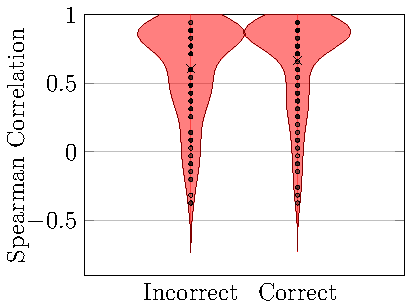
\includegraphics[width=.3\textwidth]{Figures/sec4_4_1pt_fid_spearmans.pdf}
    %                 %     \caption{Violin plots of Spearman correlations of feature rankings given by LIME explainers that did (right) and did not (left) correctly classify the input they were explaining}%Point plot for LIME's local fidelity versus its explanation quality, measured via Spearman rank correlation. Points indicate means and the vertical bars at each fidelity level indicate the 95\% confidence interval for the concordancetaken over all the models that had that level of accuracy.}
    %                 %     \label{fig:lime_fidelity}
    %                 % \end{figure}
                    
    %         \begin{figure}[ht!]
    %             \centering
    %             \begin{subfigure}[t]{.28\textwidth}
    %               \centering
    %               \captionsetup{justification=centering}
    %                   \raisebox{.2cm}{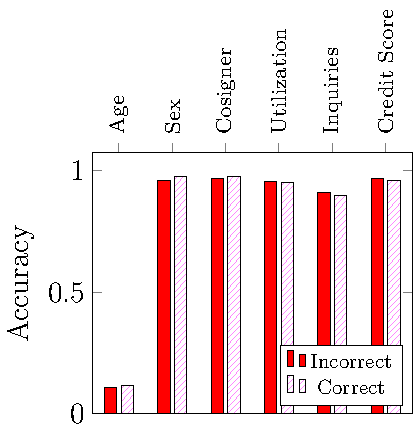
\includegraphics[width=\textwidth]{Figs/sec4_4_1pt_fid-figure0.pdf}}%{Figures/lime_shap_Spearman_magnitude.png}
    
    %               \caption{Directionality}%Spearman rank correlations of feature importance magnitudes from SHAP and LIME against the true ranking from $\mathcal{G}$. }
    %                \label{apx_fig:1pt_sign_accs}
    %             \end{subfigure}%
    %             \hspace{1cm}
    %             \begin{subfigure}[t]{.28\textwidth}
    %               \centering
    %                \captionsetup{justification=centering}
    %               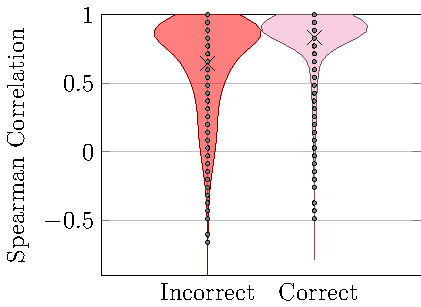
\includegraphics[width=\textwidth]{Figs/sec4_4_1pt_fid-figure1.pdf}%{Figures/lime_shap_Spearman_signed.png}
    %               \caption{Concordance}%Spearman rank correlations of signed feature importance from SHAP and LIME against the true ranking from $\mathcal{G}$.}
    %                \label{apx_fig:1pt_spearmans}
    %             \end{subfigure}
    %             \hspace{1cm}
    %             \begin{subfigure}[t]{.28\textwidth}
    %               \centering
    %             \captionsetup{justification=centering}
    %             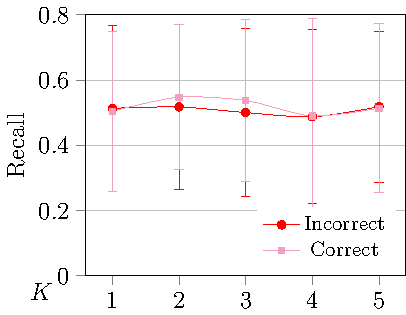
\includegraphics[width=\textwidth]{Figs/sec4_4_1pt_fid-figure2.pdf}%
    %             \caption{Relevance}%The average and standard error of recall of SHAP and LIME when attempting to capture the top K most important features to $\mathcal{G}$ when explaining $\mathcal{M}$, for varied $K=1,2,3,...$ number of features.}
    %             \label{apx_fig:1pt_recalls}
    %             \end{subfigure}
    %             \caption{Comparisons of results for our three metrics for LIME explainers whose surrogate models do and do not correctly classify the loan decision of applicants they are explaining.}
    %            \label{apx_fig:1pt_fid}
    %         \end{figure} 
        
        
    %         % Intuition dictates that as the local fidelity of the surrogate model of an explainer $\mathcal{E}$ increases, the quality of the explanations from $\mathcal{E}$ should also increase. Assuming that $\mathcal{M}$ is a good representation of $\mathcal{G}$, this sets $\mathcal{E}$ up to also represent $\mathcal{G}$ well. Although there generally seems to be a positive correlation between local fidelity and average explanation quality, the wild variance of explanation quality, especially for lower local fidelities, makes this relationship less clear. We hypothesize that the lack of clarity here is related to the fact that LIME regressors are fit on sampled data, some of which may be out of distribution \citep{rahnama19shift}.
            
    %         %It is not clear, however, what the impact of the fidelity of $\mathcal{E}$ is on explanation quality aside from very low and very high fidelities making explanation quality vary wildly. We hypothesize that the lack of clarity here is related to the fact that LIME regressors are fit on sampled data, some of which may be out of distribution \citep{rahnama19shift}.
        
    
        
            
   
    
    % %\subsection{Mitigation Strategies for Inconsistency} 
    % %    \label{sec:inconsistency_mitigation}
 
    

    %     % \subsubsection{Increasing LIME's Local Fidelity}
    %     %     In Section \ref{apx_sec:e_fidelity} we established an association between the quality of a LIME explainer $\mathcal{E}$'s explanation of $y=\mathcal{M}(\boldsymbol{\xi})$ and whether $\mathcal{E}(\boldsymbol{\xi}) = y$. We will explore here whether the accuracy of $\mathcal{E}$ on data in $\text{B}_\nu(\boldsymbol{\xi})$, the neighborhood of data samples within $\nu$ of $\boldsymbol{\xi}$. 

    %     %\subsubsection{Weak Learner LIMEs}

    %     % \subsubsection{Pearl's Backdoor Adjustment}
    %     %     \label{sec:backdoor_adjustment}

    % %n -> i
    % % add closed form for SHAP
    
    

    
    
  
  
 
        \subsubsection{Voting Ensembles}
            Prior experiments handled ensembles of explanations by constructing the final ranking by ranking the features according to the average importance given to them over the component explanations. We hypothesized that this strategy could be improved by adding sophistication using voting strategies such as the Borda count. 
            
            The Borda count is a ranked choice voting method. In it, every voter provides a ranking of the candidates. Each candidate is allocated a number of points from every ballot depending on what rank they were assigned. The point assignment method varies, but in the original formulation (which is used by the Slovenian Parliament), every candidate gets at least one point from each ballot. If there are $C$ candidates, then each voter gives their top ranked candidate $C$ points, givers their runner-up $C-1$ points, and so on until they give their lowest ranked candidate $1$ point. The candidate with the most total points wins the election.

            The Borda count can be used to produce feature rankings for an input from LIME by making many LIME explainers (by varying its hyperparameters) and considering each LIME explainer to be a voter. We tested this method by comparing single explanations for each applicant with explanations formed from the Borda count results of 100 LIME explainers with random seeds $1,2,\ldots,100$.
            
             We show the results of our experiment for concordance and relevance metrics in Figure \ref{apx_fig:borda_results} (since the Borda count operates on rankings, it is not possible to compute directionality). Overall, our experiment did not provide evidence that the Borda count is an effective way to aggregate feature rankings. In fact, the concordance of rankings constructed via the Borda count were strictly worse than those from the individual LIME explanations; Figure \ref{apx_fig:borda_spearmans} shows that the mean concordance of the rankings constructed via Borda count is less than half of that of the individual LIME rankings.

            \begin{figure}[ht!]
                \centering
                \begin{subfigure}[t]{.28\textwidth}
                  \centering
                   \captionsetup{justification=centering}
                  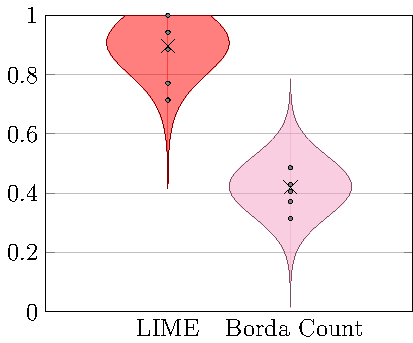
\includegraphics[width=\textwidth]{AppendixFigures/apx_borda-figure0.pdf}%{Figures/lime_shap_Spearman_signed.png}
                  \caption{Concordance}%Spearman rank correlations of signed feature importance from SHAP and LIME against the true ranking from $\mathcal{G}$.}
                   \label{apx_fig:borda_spearmans}
                \end{subfigure}
                \hspace{1cm}
                \begin{subfigure}[t]{.28\textwidth}
                  \centering
                \captionsetup{justification=centering}
                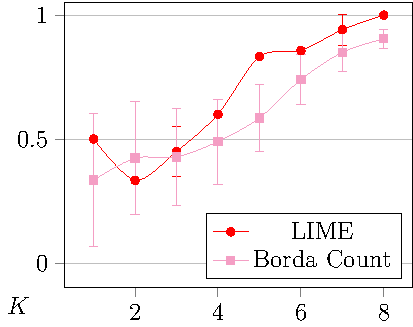
\includegraphics[width=\textwidth]{AppendixFigures/apx_borda-figure1.pdf}%
                \caption{Relevance}%The average and standard error of recall of SHAP and LIME when attempting to capture the top K most important features to $\mathcal{G}$ when explaining $\mathcal{M}$, for varied $K=1,2,3,...$ number of features.}
                \label{apx_fig:borda_recalls}
                \end{subfigure}
                \caption{Comparisons of results for our three metrics for rankings from one LIME explainer compared with rankings obtained by applying the Borda count to rankings from 100 LIME explainers.}
               \label{apx_fig:borda_results}
            \end{figure} 

        
        
    \pagebreak
    
    \section*{Appendix C: Data for Econometric Case Study}
        \label{apx_sec:econometric_details} 
        The meaning and ranges of each feature of the dataset are provided  below in Table \ref{apx_tab:case_study_features}. The meanings of the feature names were obtained \citep{HunterWilliamC1996Tcah}.
        
        \begin{table}[ht!]
            \centering
            \begin{tabular}{l|l|l}
            \toprule
            \textsc{Feature} & \textsc{Meaning}                   & \textsc{Range}                \\ \toprule
            %gdlin            & credit history meets guidelines    & binary                        \\ \hline
            good credit            & credit history meets guidelines    & binary                        \\ \hline
            %typur            & type of purchaser of loan          & 0,1,2,\textbackslash{}ldots,9 \\ \hline
            purchaser type            & type of purchaser of loan          & 0,1,2,$\ldots$,9 \\ \hline
            %inson            & \makecell{approved for private mortage insurance (PMI)}                      & binary                        \\ \hline
            PMI approved            & \makecell[l]{approved for private mortage insurance (PMI)}                      & binary                        \\ \hline
            %prop             & type of property                   & binary                        \\ \hline
            multi family     & \makecell[l]{purchasing 2-4 family home \\ versus 1 family home or condo } & binary \\ \hline
            unver            & unverifiable info                  & binary                        \\ \hline
            %fixadj           & fixed or adjustable rate           & binary                        \\ \hline
            fixed rate           & fixed or adjustable rate           & binary                        \\ \hline
            %pubrec           & filed bankruptcy                   & binary                        \\ \hline
            bankruptcy           & filed bankruptcy                   & binary                        \\ \hline
            %vr               & tract vac rte \textgreater msa med & binary                        \\ \hline
            value rate               & \makecell[l]{whether the rental income in tract \\ divided by estimate of value \\\ of rental property $>$ Boston median} & binary                        \\ \hline
            %obrat            & \makecell{percentages of housing expenditures \\ and other obligations \\ normalized by total income}    & {[}0,100{]}                   \\ \hline
            debt rate           & \makecell[l]{percentages of housing expenditures \\ and other obligations \\ normalized by total income}    & {[}0,100{]}                   \\ \hline
            old              & applicant age $>$ Boston median & binary                        \\ \hline
            married          & if applicant married               & binary                        \\ \hline
            gift             & gift as down payment               & binary                         \\
            \bottomrule
            \end{tabular}
            \caption{Feature meanings and ranges for the case study}
            \label{apx_tab:case_study_features}
        \end{table}

%\subsection{Guidance For Use of post hoc Explainers}
%    \subsubsection{Compare Explanations With Those From Decision Trees}

  

    
    
    \section*{Appendix D: Repetition of Main Experiments on Another Dataset}
        \label{apx_sec:marketing}
        To further support our findings, repeat the experiments in Section \ref{sec:causes_of_misalignment} using a synthetic direct marketing example. The meanings of the features and how they were generated is summarized in Table \ref{apx_tab:marketing_simulated}. Unlike the loan application dataset used in the main body of the paper, this direct marketing dataset contains categorical features. We binarize the categorical features, which contributes to this dataset having more features than the loan application dataset (16 versus 10). 

\begin{table}[ht!]
\centering
\resizebox{\textwidth}{!}{%
\begin{tabular}{l|l|l}
\toprule
\textsc{Feature} & \textsc{Explanation}                           & \textsc{Formula}       \\ \toprule
Age              & Customer Age                                   & Uniform(18,100)        \\ 
Sex              & Customer Sex                                   & Bernoulli(.5)          \\
Married          & Customer Marital Status                        & Bernoulli(.5)          \\ 
Education           & Customer Education Level                                & High School, College, or Graduate \\ 
Previous Purchase        & Whether product previously purchased                      & Bernoulli(.5)          \\ 
Website Visits         & Number of Times Website Visited & Uniform(0,50)         \\ 
Subscribed      & Subscribed to Regular Ads            & Bernoulli(.5)           \\ 
Offer Type     & Type of offer in Ad  & Discount, BOGO, or Free Shipping \\
Offer Value    & Value of offer in Ad & Depends on Subscription status          \\ 
Mode     & Way advertisement is delivered & Email, SMS, or Social Media \\            \bottomrule
\end{tabular}%
}
\caption{Description of features for simulated direct marketing data.}
\label{apx_tab:marketing_simulated}
\end{table}
        \subsubsection{Baseline}
            Figure \ref{apx_fig:marketing_beta_alignment} shows a comparison between SHAP and LIME with their default settings and a random explainer when explaining a model with test set ROC AUC of .93 that was trained on the marketing dataset described in Table \ref{apx_tab:marketing_simulated}. We reach the same conclusion as in Section \ref{sec:misalignment}, that is that LIME does fairly well with respect to all three metrics while SHAP is not significantly better than a random explainer except with respect to relevance.
            
            \begin{figure}[ht!]
                \centering
                \begin{subfigure}[t]{.28\textwidth}
                  \centering
                  \captionsetup{justification=centering}
                      \raisebox{.2cm}{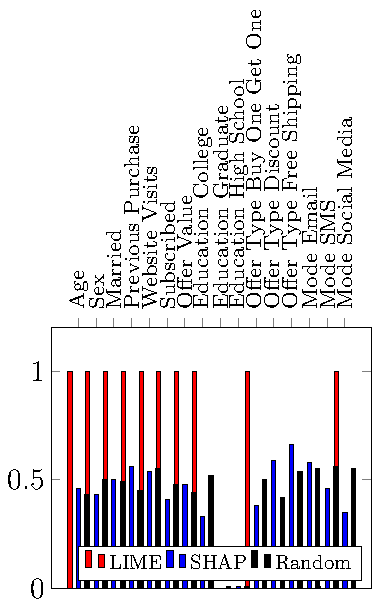
\includegraphics[width=\textwidth]{MarketingFigs/sec4_1-figure0.pdf}}%{Figures/lime_shap_Spearman_magnitude.png}
    
                  \caption{Directionality}%Spearman rank correlations of feature importance magnitudes from SHAP and LIME against the true ranking from $\mathcal{G}$. }
                   \label{apx_fig:lime_shap_sign_accs}
                \end{subfigure}%
                \hspace{1cm}%\hfill
                \begin{subfigure}[t]{.28\textwidth}
                  \centering
                   \captionsetup{justification=centering}
                  \raisebox{.05cm}{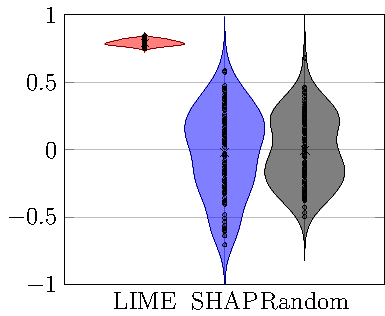
\includegraphics[width=\textwidth]{MarketingFigs/sec4_1-figure1.pdf}}%{Figures/lime_shap_Spearman_signed.png}
                  \caption{Concordance}%Spearman rank correlations of signed feature importance from SHAP and LIME against the true ranking from $\mathcal{G}$.}
                   \label{apx_fig:lime_shap_Spearman_signed}
                \end{subfigure}
                \hspace{1cm}%\hfill
                \begin{subfigure}[t]{.28\textwidth}
                  \centering
                   \captionsetup{justification=centering}
                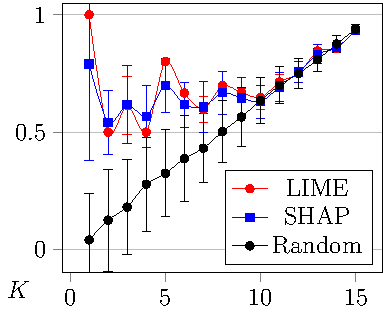
\includegraphics[width=\textwidth]{MarketingFigs/sec4_1-figure2.pdf}%
                \caption{Relevance}%The average and standard error of recall of SHAP and LIME when attempting to capture the top K most important features to $\mathcal{G}$ when explaining $\mathcal{M}$, for varied $K=1,2,3,...$ number of features.}
                \label{apx_fig:avg_recall}
                \end{subfigure}
                \caption{Bar plot of directionality, violin plot of concordance, and line plot for relevance$_k$. For plot (c) each point in the line plot represents a mean relevance for a given $k$. The error bars represent the standard error. The total number of features is 16.}
               \label{apx_fig:marketing_beta_alignment}
            \end{figure}   

        \subsubsection{SHAP Normalization}
            As in Section \ref{sec:theoretical_considerations}, we check whether SHAP normalization is useful when working with the direct marketing dataset. Figure \ref{apx_fig:marketing_shap_dividex_corr} shows that this is indeed the case if not only because concordance increased greatly. Additionally, directionality for many features increased from nearly .5 to nearly 1. 


           \begin{figure}[ht!]
            \centering
            \begin{subfigure}[t]{.28\textwidth}
              \centering
              \captionsetup{justification=centering}
                  \raisebox{.2cm}{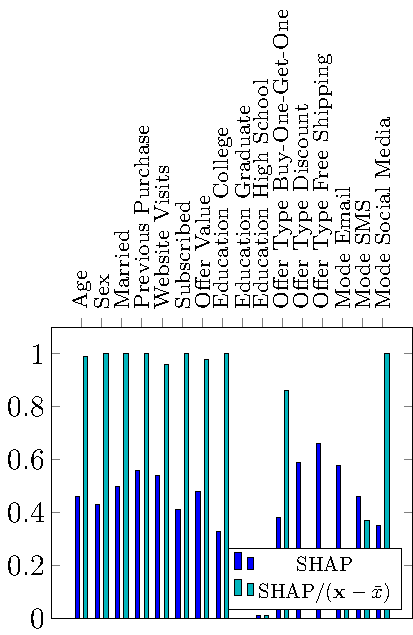
\includegraphics[width=\textwidth]{MarketingFigs/shap_dividex-figure0.pdf}}%{Figures/lime_shap_Spearman_magnitude.png}

              \caption{Directionality}%Spearman rank correlations of feature importance magnitudes from SHAP and LIME against the true ranking from $\mathcal{G}$. }
               \label{apx_fig:marketing_shap_dividex_accs}
            \end{subfigure}%
            \hspace{1cm}%\hfill
            \begin{subfigure}[t]{.28\textwidth}
              \centering
               \captionsetup{justification=centering}
              \raisebox{.05cm}{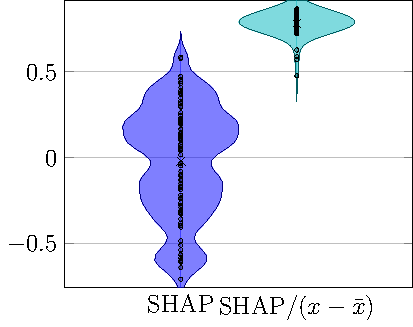
\includegraphics[width=\textwidth]{MarketingFigs/shap_dividex-figure1.pdf}}%{Figures/lime_shap_Spearman_signed.png}
              \caption{Concordance}%Spearman rank correlations of signed feature importance from SHAP and LIME against the true ranking from $\mathcal{G}$.}
               \label{apx_fig:marketing_shap_dividex_spearmans}
            \end{subfigure}
            \hspace{1cm}%\hfill
            \begin{subfigure}[t]{.28\textwidth}
              \centering
               \captionsetup{justification=centering}
            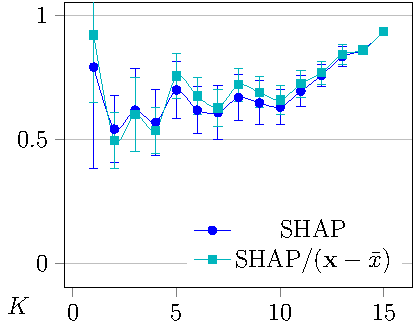
\includegraphics[width=\textwidth]{MarketingFigs/shap_dividex-figure2.pdf}%
            \caption{Relevance}%The average and standard error of recall of SHAP and LIME when attempting to capture the top K most important features to $\mathcal{G}$ when explaining $\mathcal{M}$, for varied $K=1,2,3,...$ number of features.}
            \label{apx_fig:marketing_shap_dividex_recalls}
            \end{subfigure}
            \caption{Comparison of SHAP explanations without and with SHAP value normalization}
           \label{apx_fig:marketing_shap_dividex_corr}
        \end{figure}   

        \subsubsection{Role of Predictive Performance of $\mathcal{M}$}
            To test the effect of the predictive performance of $\mathcal{M}$, we compare explanations of models $\mathcal{M}_1$ with AUC .68, $\mathcal{M}_2$ with AUC .93, and $\mathcal{M}_3$ with AUC .99. The results of our comparison, illustrated below in Figure \ref{apx_fig:marketing_mlp_auc_increase}, show that although directionality was not significantly impacted for SHAP or LIME, increasing the model AUC had substantial effects on concordance and relevance.
        \begin{figure}[t!]
            \subfloat[SHAP Directionality]{%
                \raisebox{.2cm}{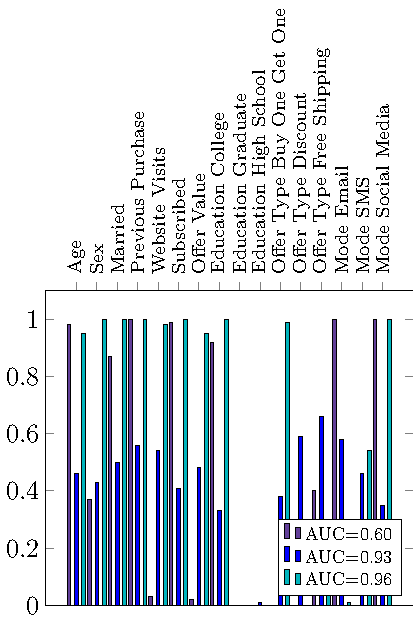
\includegraphics[width=.28\textwidth]{MarketingFigs/sec4_4_mlp_auc_shap-figure0.pdf}}%
                \label{apx_fig:marketing_mlp_avg_shap_sign_accs}%
            }\hspace{1cm}
            \subfloat[SHAP Concordance]{%
                 \raisebox{.05cm}{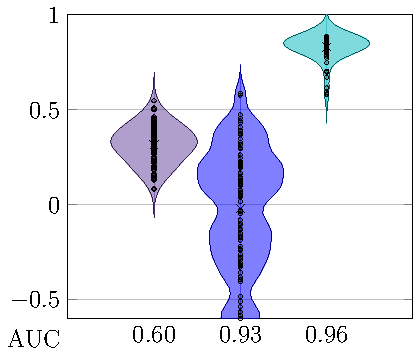
\includegraphics[width=.28\textwidth]{MarketingFigs/sec4_4_mlp_auc_shap-figure1.pdf}}%
                \label{apx_fig:marketing_mlp_auc_shap_spearmans}%
            }\hspace{1cm}
            \subfloat[SHAP Relevance]{%
                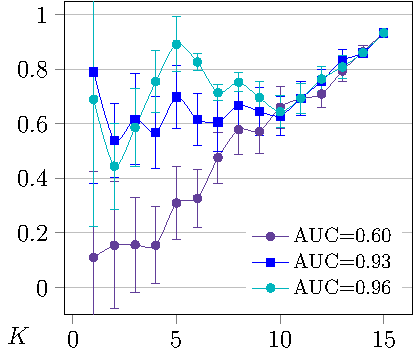
\includegraphics[width=.28\textwidth]{MarketingFigs/sec4_4_mlp_auc_shap-figure2.pdf}%
                \label{apx_fig:marketing_mlp_auc_shap_recalls}%
            }\\
            \subfloat[LIME Directionality]{%
                \raisebox{.2cm}{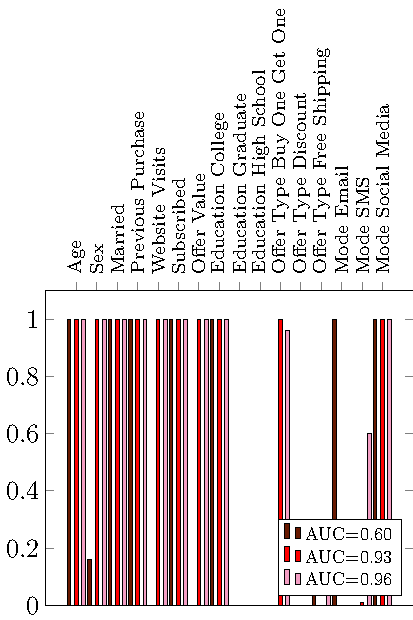
\includegraphics[width=.28\textwidth]{MarketingFigs/sec4_4_mlp_auc_lime-figure0.pdf}}%
                \label{apx_fig:marketing_mlp_auc_lime_sign_accs}%
            }\hspace{1cm}%\hfill
            \subfloat[LIME Concordance]{%
                \raisebox{.05cm}{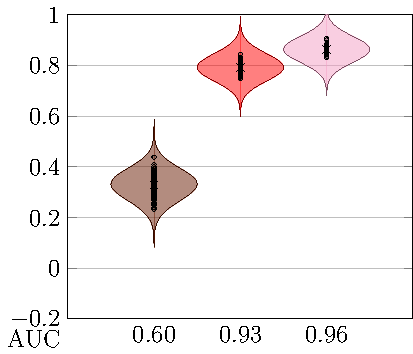
\includegraphics[width=.28\textwidth]{MarketingFigs/sec4_4_mlp_auc_lime-figure1.pdf}}%
                \label{apx_fig:marketing_mlp_auc_lime_spearmans}%
            }\hspace{1cm}
            \subfloat[LIME Relevance]{%
                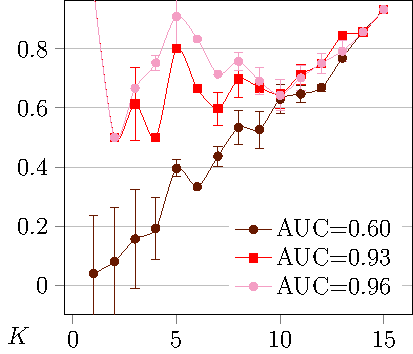
\includegraphics[width=.28\textwidth]{MarketingFigs/sec4_4_mlp_auc_lime-figure2.pdf}%
                \label{apx_fig:marketing_mlp_auc_lime_recalls}%
            }\\
            \caption{Comparisons of results for our three metrics for SHAP and LIME when explaining $\mathcal{M}_1$ with AUC=.6, $\mathcal{M}_2$ with AUC=0.92, and $\mathcal{M}_3$ with AUC=.99}
            \label{apx_fig:marketing_mlp_auc_increase}
        \end{figure}


        \subsubsection{Role of Feature Independence}
            Following Section \ref{sec:role_of_correlation}, we modify the direct marketing dataset to make the features independent but do not change the formula for $\mathcal{G}(\mathbf{X})$. The only change made is to change ``Offer Value" from being a function of subscription status to becoming uniformly distributed between 5 and 50 dollars.

            It was again the case that explanations of the model trained on data with independent features were more data aligned. In particular, Figure \ref{apx_fig:marketing_lime_shap_colinear} shows that explanations of the model trained on the version of the marketing dataset with independent features had a mean concordance which was about .1 larger and $\text{relevance}_k$ for $k=2,3,4$ which were up to .5 larger. 
            
            \begin{figure}[t!]
                \subfloat[SHAP Directionality]{%
                    \raisebox{.2cm}{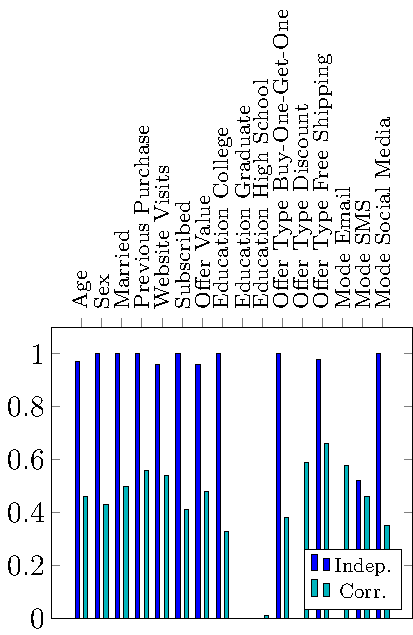
\includegraphics[width=.28\textwidth]{MarketingFigs/shap_corr-figure0.pdf}}%
                    \label{apx_fig:marketing_shap_corr_accs}%
                }\hspace{1cm}%\hfill
                \subfloat[SHAP Concordance]{%
                    \raisebox{.05cm}{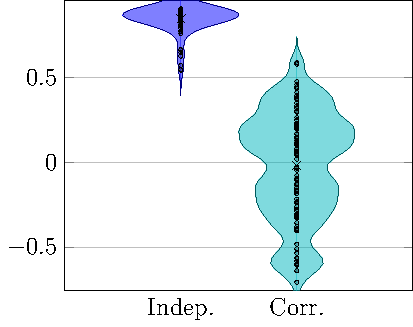
\includegraphics[width=.28\textwidth]{MarketingFigs/shap_corr-figure1.pdf}}%
                    \label{apx_fig:marketing_shap_corr_spearmans}%
                }\hspace{1cm}%\hfill
                \subfloat[SHAP Relevance]{%
                    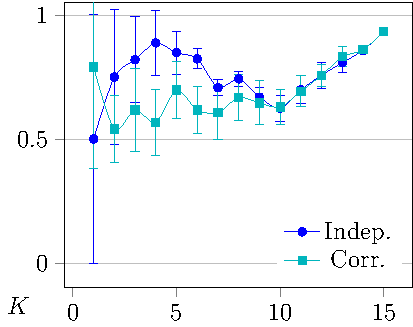
\includegraphics[width=.28\textwidth]{MarketingFigs/shap_corr-figure2.pdf}%
                    \label{apx_fig:marketing_shap_corr_recalls}%
                }\\
                \subfloat[LIME Directionality]{%
                    \raisebox{.2cm}{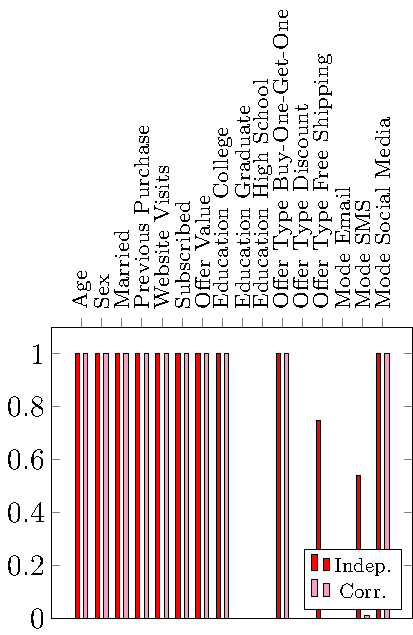
\includegraphics[width=.28\textwidth]{MarketingFigs/lime_corr-figure0.pdf}}%
                    \label{apx_fig:marketing_lime_corr_accs}%
                }\hspace{1cm}%\hfill
                \subfloat[LIME Concordance]{%
                    \raisebox{.05cm}{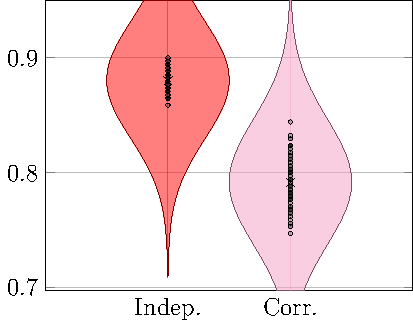
\includegraphics[width=.28\textwidth]{MarketingFigs/lime_corr-figure1.pdf}}%
                    \label{apx_fig:marketing_lime_corr_spearmans}%
                }\hspace{1cm}%\hfill
                \subfloat[LIME Relevance]{%
                    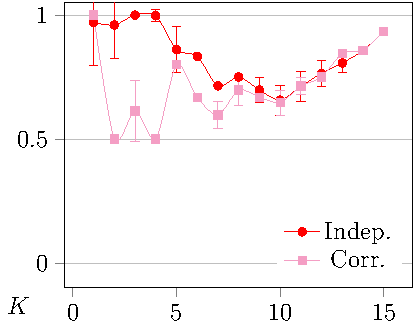
\includegraphics[width=.28\textwidth]{MarketingFigs/lime_corr-figure2.pdf}%
                    \label{apx_fig:marketing_lime_corr_recalls}%
                }\\
                \caption{Comparison of faithfulness of explanations of models trained on data with independent features versus data with two strongly correlated features.}
                \label{apx_fig:marketing_lime_shap_colinear}
            \end{figure}

        % \subsubsection{Increasing $\nu$ and $n$ for LIME}
        %     The effect of increasing $\nu$ and $n$ may not be immediately apparent from Figure \ref{apx_fig:marketing_lime_tuning}, but it does show that directionality was increased for some features and not lower for any other feature except ``website visits." Directionality for ``Offer Type: Free Shipping" was significantly increased with $p<.001$ while directionality for ``Mode: SMS" was increased insignificantly with $p\simeq.07$. Concordance was slightly lower when $\nu=n=10000$. Relevance was significantly better for $k=1,3$ with $p\simeq.004$.
        %     \begin{figure}[ht!]
        %         \centering
        %         \begin{subfigure}[t]{.28\textwidth}
        %           \centering
        %           \captionsetup{justification=centering}
        %               \raisebox{.2cm}{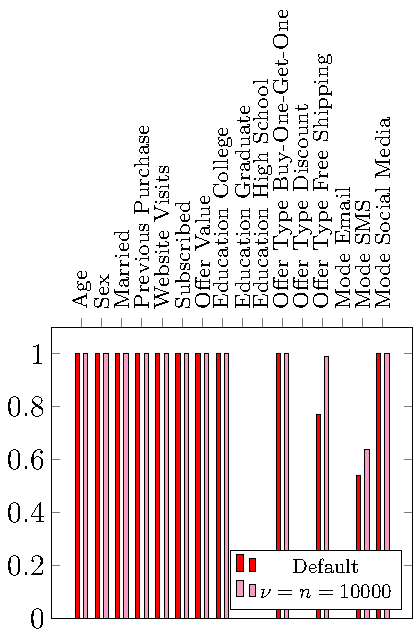
\includegraphics[width=\textwidth]{MarketingFigs/lime_nu_N-figure0.pdf}}%{Figures/lime_shap_Spearman_magnitude.png}
    
        %           \caption{Directionality}%Spearman rank correlations of feature importance magnitudes from SHAP and LIME against the true ranking from $\mathcal{G}$. }
        %            \label{apx_fig:marketing_lime_tuning_sign_accs}
        %         \end{subfigure}%
        %         \hspace{1cm}
        %         \begin{subfigure}[t]{.28\textwidth}
        %           \centering
        %            \captionsetup{justification=centering}
        %           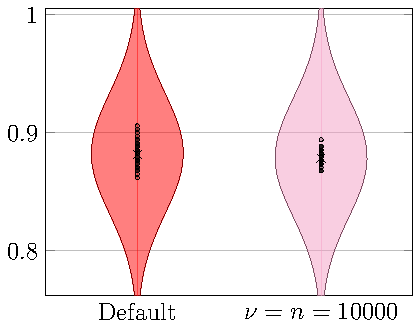
\includegraphics[width=\textwidth]{MarketingFigs/lime_nu_N-figure1.pdf}%{Figures/lime_shap_Spearman_signed.png}
        %           \caption{Concordance}%Spearman rank correlations of signed feature importance from SHAP and LIME against the true ranking from $\mathcal{G}$.}
        %            \label{apx_fig:marketing_lime_tuning_spearmans}
        %         \end{subfigure}
        %         \hspace{1cm}
        %         \begin{subfigure}[t]{.28\textwidth}
        %           \centering
        %            \captionsetup{justification=centering}
        %         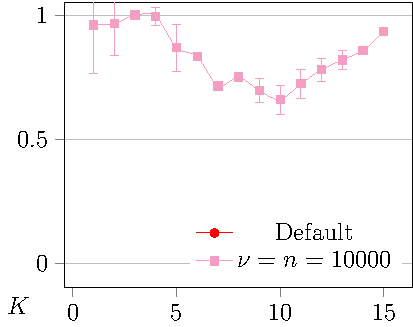
\includegraphics[width=\textwidth]{MarketingFigs/lime_nu_N-figure2.pdf}%
        %         \caption{Relevance}%The average and standard error of recall of SHAP and LIME when attempting to capture the top K most important features to $\mathcal{G}$ when explaining $\mathcal{M}$, for varied $K=1,2,3,...$ number of features.}
        %         \label{apx_fig:marketing_lime_tuning_recalls}
        %         \end{subfigure}
        %         \caption{Comparison of LIME explainer with default settings versus $\nu=n=10000$ with respect to our three metrics}
        %        \label{apx_fig:marketing_lime_tuning}
        %     \end{figure} 

        
        % \subsubsection{Averaging Explanations of One Model by Different Explainers}
        %     We again tested whether averaging the explanations of one model by 10 LIME explainers with different random seeds was useful. The results of the experiment are given in Figure \ref{apx_fig:marketing_mlp_auc_increase} and show that directionality increased appreciably for a few features while it was unchanged for the others, there was not a significant change to concordance, and there was some improvement to relevance for small $k$. 

        %     Indeed, for directionality, ``Mode: SMS" was increased with $p\simeq .01$, ``Offer Type: Free Shipping" increased with $p<.001$, and the other features were unaffected except for ``Website Visits" which was worse with $p<.001$. Relevance was significantly increased for $k=1$  with $p\simeq .004$.% and insignificantly increased for $k=3$ with $p\simeq .07$. 

        %     % The strategy increased the consistency in some respects. Feature importance signs were more consistent with $p\simeq .1$ for ``Mode: SMS" and significantly more consistent for ``Offer Type: Free Shipping" with $p<.001$. The rankings were significantly more consistent with $p<.001$. 
        %     \begin{figure}[!h]
        %     \centering
        %         \begin{subfigure}[t]{0.28\textwidth}
        %         \centering
        %         \raisebox{.2cm}{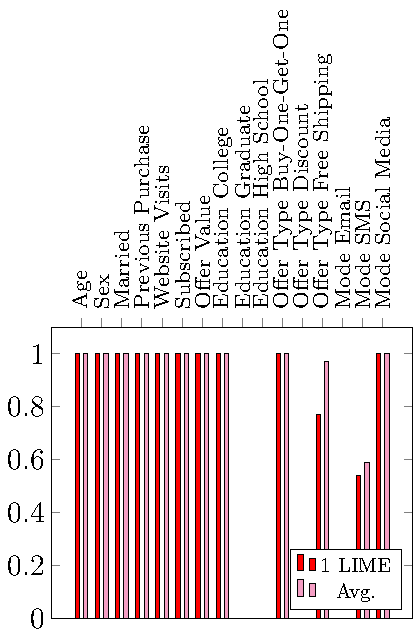
\includegraphics[width=\textwidth]{MarketingFigs/lime_avg-figure0.pdf}}
        %         \caption{Directionality} \label{apx_fig:marketing_lime_avg_sign_accs}
        %     \end{subfigure}\hspace{1cm}
        %     \begin{subfigure}[t]{0.28\textwidth}
        %         \centering
        %         \raisebox{.05cm}{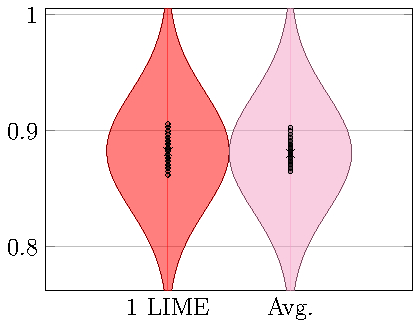
\includegraphics[width=\textwidth]{MarketingFigs/lime_avg-figure1.pdf}}
        %         \caption{Concordance} \label{apx_:marketing_lime_avg_spearmans}
        %     \end{subfigure}\hspace{1cm}
        %      \begin{subfigure}[t]{0.28\textwidth}
        %         \centering
        %         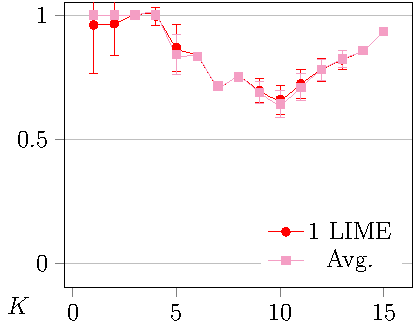
\includegraphics[width=\textwidth]{MarketingFigs/lime_avg-figure2.pdf}
        %         \caption{Relevance}
        %         \label{apx_fig:marketing_lime_avg_recalls}
        %     \end{subfigure}
        %     \caption{Comparisons of results for our three metrics for  explanations of an NN $\mathcal{M}$ by 1 LIME explainer versus those created by averaging the feature importance values of 100 LIME explanations of $\mathcal{M}$}\label{apx_fig:marketing_lime_avg}
        %     \end{figure}

        
        
        % \subsubsection{Averaging Explanations of Different Models}
        %     The models we used for averaging all had test set AUCs of .96 and test set accuracies of .89. It is easily seen from the visualization of the experimental results in Figure \ref{apx_fig:marketing_mlp_increase} that this strategy was beneficial because the concordances are noticeably larger for both SHAP and LIME. 

        %     With regard to directionality for SHAP, ``Offer Type: Free Shipping" and ``Website visits" were the two features that significantly increased, as they had $p<.001$. Concordance significantly increased with $p<.001$. Relevance was significantly increased for $k=1,12$. It also increased for the other $k$, but not significantly at the $\alpha=.05$ level. 
            
        %     \begin{figure}[t!]
        %         \subfloat[SHAP Directionality]{%
        %             \raisebox{.2cm}{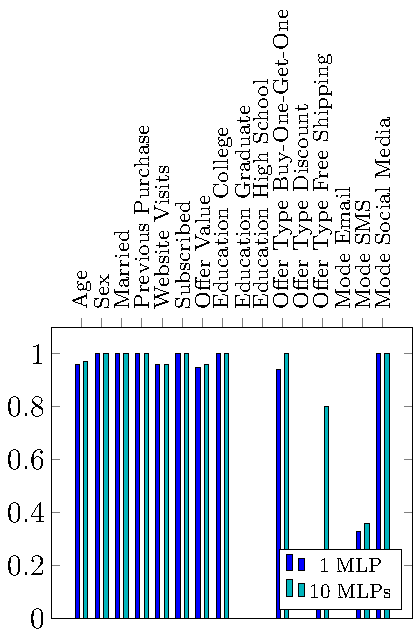
\includegraphics[width=.28\textwidth]{MarketingFigs/shap_mlp_avg-figure0.pdf}}%
        %             \label{apx_fig:marketing_mlp_avg_shap_sign_accs}%
        %         }\hspace{1cm}
        %         \subfloat[SHAP Concordance]{%
        %             \raisebox{.05cm}{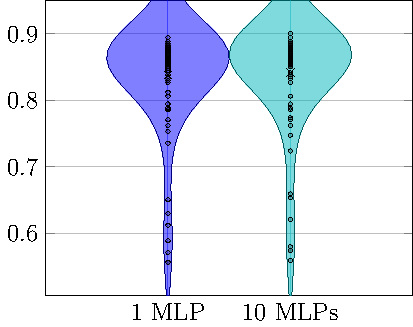
\includegraphics[width=.28\textwidth]{MarketingFigs/shap_mlp_avg-figure1.pdf}}%
        %             \label{apx_fig:marketing_mlp_avg_shap_spearmans}%
        %         }\hspace{1cm}
        %         \subfloat[SHAP Relevance]{%
        %             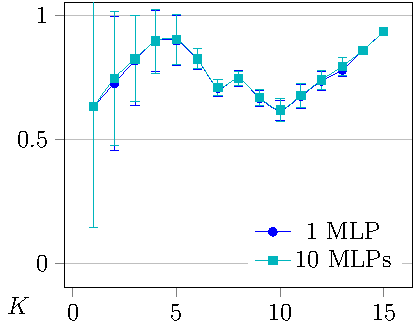
\includegraphics[width=.28\textwidth]{MarketingFigs/shap_mlp_avg-figure2.pdf}%
        %             \label{apx_fig:marketing_mlp_avg_shap_recalls}%
        %         }\\
        %         \subfloat[LIME Directionality]{%
        %             \raisebox{.2cm}{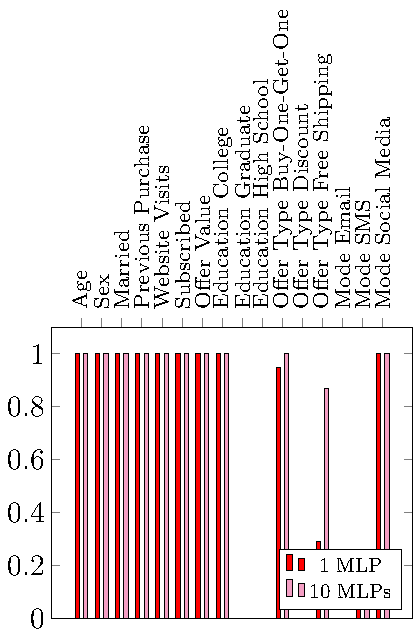
\includegraphics[width=.28\textwidth]{MarketingFigs/lime_mlp_avg-figure0.pdf}}%
        %             \label{apx_fig:marketing_mlp_avg_lime_sign_accs}%
        %         }\hspace{1cm}
        %         \subfloat[LIME Concordance]{%
        %             \raisebox{.05cm}{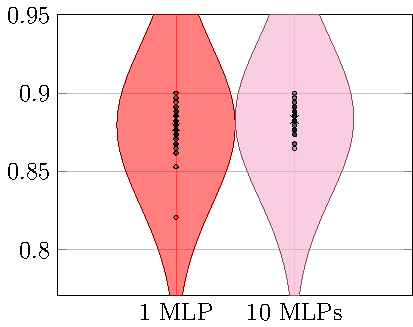
\includegraphics[width=.28\textwidth]{MarketingFigs/lime_mlp_avg-figure1.pdf}}%
        %             \label{apx_fig:marketing_mlp_avg_lime_spearmans}%
        %         }\hspace{1cm}
        %         \subfloat[LIME Relevance]{%
        %             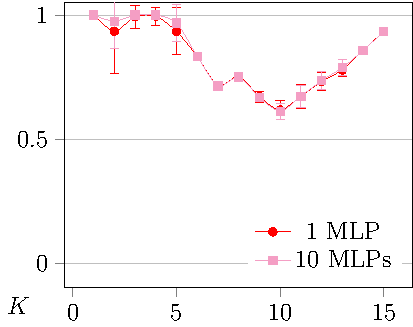
\includegraphics[width=.28\textwidth]{MarketingFigs/lime_mlp_avg-figure2.pdf}%
        %             \label{apx_fig:marketing_mlp_avg_lime_recalls}%
        %         }\\
        %         \caption{Comparisons of results for our three metrics for SHAP (top row) and LIME (bottom row) explanations of 1 NN versus explanations constructed by averaging the feature importance values of 10 NNs.}
        %         \label{apx_fig:marketing_mlp_increase}
        %     \end{figure}

        
        
        % \subsubsection{Optimizing the Tradeoff between Complexity and Predictive Power}
        %     In this section we compare the data-alignment of explanations of models $\mathcal{M}_1$ with 100 neurons in its hidden layer and $\mathcal{M}_2$ with only 2 nodes in its hidden layer. Both models have a test set AUC of about .96. We found that the explanations of the simpler model $\mathcal{M}_2$ were more data-aligned with respect to relevance but less data-aligned with respect to concordance. Figure \ref{apx_fig:marketing_decreasing_complexity} shows that the mean relevances for both SHAP and LIME were noticeably larger for $\mathcal{M}_2$ for many $k$ but the mean concordances for both SHAP and LIME were smaller for explanations of $\mathcal{M}_2$ than for explanations of $\mathcal{M}_1$.

        %     For SHAP, directionality was significantly improved for ``Mode: Email", ``Mode: SMS", and ``Offer Type: Free Shipping" with $p<.001$. Directionality for SHAP explanations of $\mathcal{M}_2$ was not significantly lower for any feature. Relevance was significantly improved for $k=1$ with $p\simeq .01$, $k=2$ with $p\simeq .04$, $k=5,\ldots,13$ with $p<.001$, and $k=14$ with $p\simeq .002$.  For LIME, directionality was also significantly improved for ``Mode: Email", ``Mode: SMS", and ``Offer Type: Free Shipping" with $p<.001$ and not significantly lower for any feature. Directionality was significantly improved for $k=6$ with $p\simeq .02$ and for $k=7,\ldots,14$ with $p<.001$. 

            
        %     \begin{figure}[t!]
        %         \subfloat[SHAP Directionality]{%
        %             \raisebox{.2cm}{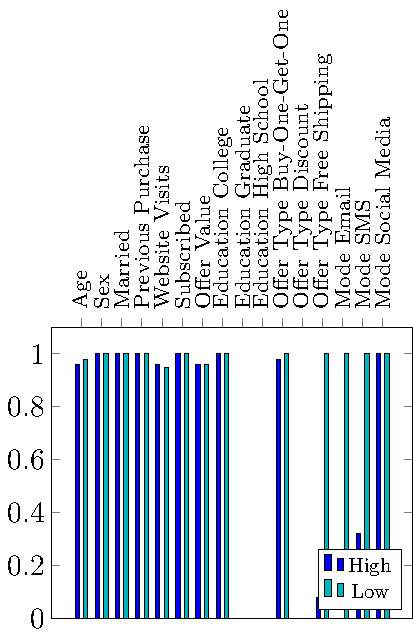
\includegraphics[width=.28\textwidth]{MarketingFigs/shap_cplx-figure0.pdf}}%
        %             \label{apx_fig:marketing_decreasing_complexity_shap_sign_accs}%
        %         }\hspace{1cm}
        %         \subfloat[SHAP Concordance]{%
        %             \raisebox{.05cm}{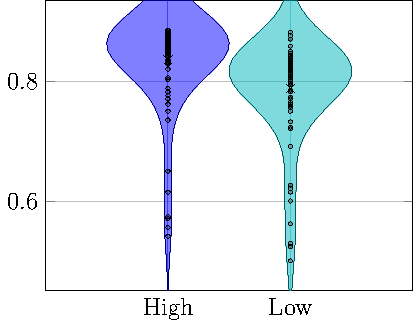
\includegraphics[width=.28\textwidth]{MarketingFigs/shap_cplx-figure1.pdf}}%
        %             \label{apx_fig:marketing_decreasing_complexity_shap_spearmans}%
        %         }\hspace{1cm}
        %         \subfloat[SHAP Relevance]{%
        %             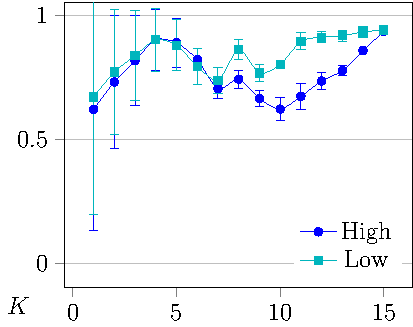
\includegraphics[width=.28\textwidth]{MarketingFigs/shap_cplx-figure2.pdf}%
        %             \label{apx_fig:marketing_decreasing_complexity_shap_recalls}%
        %         }\\
        %         \subfloat[LIME Directionality]{%
        %             \raisebox{.2cm}{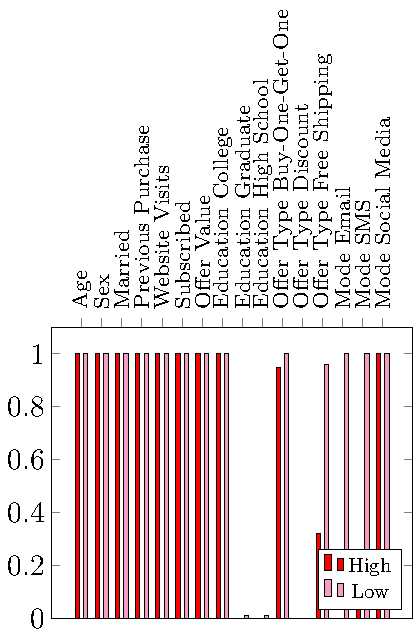
\includegraphics[width=.28\textwidth]{MarketingFigs/lime_cplx-figure0.pdf}}%
        %             \label{apx_fig:marketing_decreasing_complexity_lime_sign_accs}%
        %         }\hspace{1cm}
        %         \subfloat[LIME Concordance]{%
        %             \raisebox{.05cm}{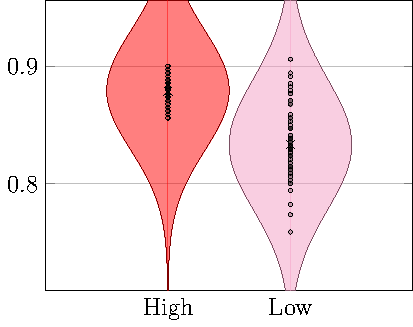
\includegraphics[width=.28\textwidth]{MarketingFigs/lime_cplx-figure1.pdf}}%
        %             \label{subfig:marketing_decreasing_complexity_lime_spearmans}%
        %         }\hspace{1cm}
        %         \subfloat[LIME Relevance]{%
        %             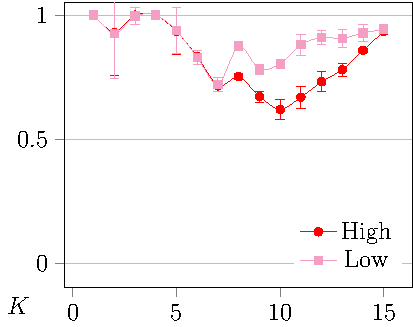
\includegraphics[width=.28\textwidth]{MarketingFigs/lime_cplx-figure2.pdf}%
        %             \label{apx_fig:marketing_decreasing_complexity_lime_recalls}%
        %         }\\
        %         \caption{Comparisons of results for our three metrics for SHAP (top row) and LIME (bottom row) explanations of equally accurate NNs with high and low complexity.}
        %         \label{apx_fig:marketing_decreasing_complexity}
        %     \end{figure}


    



    
   




\end{document}
% %%%%%%%%%%%%%%%%%?